\documentclass[11pt,a4paper]{article}
\usepackage[T1]{fontenc}
\usepackage[utf8]{inputenc}
\usepackage{lmodern,microtype,amsmath,amssymb,amsthm,mathtools}
\usepackage[a4paper,margin=25mm,headheight=15pt]{geometry}
\usepackage{booktabs,longtable,array,enumitem,xcolor,tikz,fancyhdr,listings,fancyvrb,needspace}
\usepackage{tocloft}
\setlength{\cftsecnumwidth}{4em}
\setlength{\cftsubsecindent}{4em}
\setlength{\cftsubsecnumwidth}{4.7em}
\definecolor{ink}{HTML}{183447}
\definecolor{accent}{HTML}{087F8C}
\definecolor{primefive}{HTML}{B95C25}
\definecolor{codebg}{HTML}{F4F6F7}
\usepackage[colorlinks=true,linkcolor=ink,citecolor=accent,urlcolor=accent,breaklinks=true]{hyperref}
\renewcommand{\theHsection}{\Roman{part}.\arabic{section}}
\usetikzlibrary{arrows.meta,calc}
\newtheorem{theorem}{Theorem}[section]
\newtheorem{lemma}[theorem]{Lemma}
\newtheorem{proposition}[theorem]{Proposition}
\newtheorem{corollary}[theorem]{Corollary}
\newtheorem{conjecture}[theorem]{Conjecture}
\theoremstyle{definition}
\newtheorem{definition}[theorem]{Definition}
\newtheorem{question}[theorem]{Question}
\newtheorem{problem}[theorem]{Problem}
\newtheorem{observation}[theorem]{Reported computation}
\newtheorem{example}[theorem]{Example}
\theoremstyle{remark}
\newtheorem{remark}[theorem]{Remark}
\numberwithin{equation}{section}
\DeclareMathOperator{\CT}{CT}
\DeclareMathOperator{\ord}{ord}
\DeclareMathOperator{\lcm}{lcm}
\newcommand{\Q}{\mathbb Q}\newcommand{\Z}{\mathbb Z}
\newcommand{\N}{\mathbb N}\newcommand{\R}{\mathbb R}\newcommand{\C}{\mathbb C}
\newcommand{\Qb}{\overline{\mathbb Q}}
\setlength{\parindent}{0pt}\setlength{\parskip}{4pt}
\setlength{\emergencystretch}{3em}
\setlist{nosep,leftmargin=*,topsep=4pt}
\lstset{basicstyle=\ttfamily\footnotesize,breaklines=true,
 columns=fullflexible,keepspaces=true,showstringspaces=false,
 backgroundcolor=\color{codebg},frame=single,rulecolor=\color{black!15},
 xleftmargin=4pt,xrightmargin=4pt,aboveskip=8pt,belowskip=8pt}
\pagestyle{fancy}\fancyhf{}
\fancyhead[L]{\small\sffamily Recurrences, Differences, and Collatz Orbits}
\fancyhead[R]{\small\sffamily Unified research manuscript}
\fancyfoot[C]{\thepage}
\renewcommand{\headrulewidth}{0.3pt}
\hypersetup{pdftitle={Recurrences, Absolute Differences, and Collatz Orbits: Algebra, Prime Patterns, and Zero Distributions},pdfauthor={KEIO; research development with AI assistance}}
\title{\sffamily\bfseries\color{ink}Recurrences, Absolute Differences,\\and Collatz Orbits\\[8pt]\large Algebra, Prime Patterns, and Zero Distributions}
\author{KEIO\\\small Research development and manuscript preparation with AI assistance}
\date{Unified and extended research edition --- 24 October 2026}
\begin{document}
\maketitle
\begin{abstract}
We bring together recurrence-order arguments for binomial-power sums,
extremal finite absolute-difference triangles, explicitly constructed Collatz
trajectories, and the algebra and geometry of their orbit polynomials.
The collection includes proposed solutions to precisely stated problems
from the literature, proofs of auxiliary classification results, and explicit
boundaries between theorems, conditional statements, and numerical evidence.
For terminating Collatz polynomials we study the zero accumulation annulus,
prime-dependent arithmetic separation, logarithmic independence, and
Euler--Mascheroni boundary-distance limits. A further extension determines
maximal Kummer kernels for an odd-degree family and its entire power-of-two
radical tower, while a deterministic inverse-orbit construction realizes
prescribed rotationally invariant zero distributions. All proofs,
finite-certificate procedures, figures, and references needed by the
stated arguments are contained in this source. No universal Collatz
termination, prime Gilbreath conjecture, twin-prime conjecture, Mersenne-prime
infinitude, or unresolved constant's transcendence is asserted.
\end{abstract}
\paragraph{Status.}
This is an AI-assisted research manuscript, not an externally peer-reviewed
publication. Statements presented as proved are supported by the arguments
in this document; historical priority and acceptance by the mathematical
community have not been established. A supplied large computational census
is not reclassified as an independently rerun proof. Such observations are
marked separately wherever no complete certificate has been retained.
\paragraph{Single-source format.}
The PDF and its one English \LaTeX{} file are the complete deliverable.
No companion Python file, data archive, bibliography database, or external
figure is required. Ordinary mathematical citations are scholarly dependencies.
Inline programs are reproducibility aids; compilation does not execute them.
\clearpage
{\small\setlength{\parskip}{0pt}\setcounter{tocdepth}{2}\tableofcontents}
\clearpage
\section*{Reading guide and scope of the consolidation}
\addcontentsline{toc}{section}{Reading guide and scope of the consolidation}
Part~I develops recurrence and finite-difference methods and prime-pattern
constructions. Part~II applies them to specific questions from the literature,
retaining the exact scope of partial and negative answers. Part~III assembles
the zero geometry and arithmetic results. Part~IV develops full Galois groups
and limiting zero distributions and contains the principal further extensions.
The parts use a common bibliography and globally distinct references; their
local definitions are retained when the meaning of a symbol changes.

The unaccelerated Collatz map is denoted $C$, the shortcut map $T$, and the
odd-to-odd map $S$ in Part~I. Part~II sometimes writes $c$ for the shortcut
map and uses its own local trajectory notation. Throughout, an orbit
polynomial ends at the \emph{first} occurrence of $1$. Statements about a
full polynomial apply only when that starting value is known to terminate.
This restriction is not an assumption that the Collatz conjecture holds.
The symbol $P_a$ in the inverse-Mersenne family of Part~I denotes an integer,
whereas $P_N(z)$ denotes an orbit polynomial elsewhere.

The recurrence order of a Franel sequence refers to rational-function
coefficients and shift width, not the degree of the polynomial coefficients.
Finite Gilbreath extension questions are distinct from Gilbreath's conjecture
for the actual primes. Prime-chain existence varies an affine parameter;
it does not guarantee a new prime above a prescribed fixed giant seed.
Zero accumulation as a set is distinct from weak convergence of full root
counting measures. These distinctions are used throughout the proofs.

For the large finite searches inherited from the problem-oriented source,
the present edition records whether a displayed claim is an analytic theorem,
an explicit finite certificate, or reported exploratory evidence. The latter
does not establish a universal conjecture. The main analytic statements do
not rely on the exploratory searches.

\paragraph{Further results established in this edition.}
The main additions beyond the supplied sources are the following.
\begin{enumerate}
\item Theorem~\ref{D:thm:full-lifting} removes the former order-of-$2$
restriction from the full radical-tower calculation: it holds for every
odd $k\ge3$ with $5\nmid k$. For prime $k\ge23$ with $11\nmid k+1$,
the full Collatz-polynomial group is $(C_4)^k\rtimes(S_k\times C_2)$.
\item Theorem~\ref{D:thm:improved-radial-band} realizes every rotationally
invariant probability measure on $2\,3^{-2/7}\le|z|\le2$, improving the
earlier endpoint $2\,3^{-1/4}$. The uniform two-inverse-step exponent
cost $7$ is optimal, although the resulting radial endpoint need not be.
\item Theorem~\ref{B:P:thm:infinite-first-prime} gives infinitely many
odd composite starts whose first prime is any prescribed prime other
than $3$, with explicit arrival times and a logarithmic counting bound.
\item Corollary~\ref{A:cor:all-mersenne-shaped-divisors} completes the
even-exponent Mersenne-shaped divisor classification. Theorem~\ref{C:thm:ominimal-prefix}
extends the fixed-prefix prime-only obstruction to o-minimal rules,
including fixed expressions using real exponentials and logarithms.
\end{enumerate}
These are explicit extensions and auxiliary classifications. They are not
presented as resolutions of the famous conjectures excluded above. The
additional $G_2$ shift-filter rigidity result appears in
Theorem~\ref{B:F:thm:filter-rigidity}.

\clearpage
\part{Recurrences, finite differences, and prime orbit families}\label{part:A}
\setcounter{section}{0}
\renewcommand{\thesection}{I.\arabic{section}}
\section{Framework and conventions}
The starting point is the binomial-power sequence
\[
A_s(n)=\sum_{k=0}^n\binom nk^s,\qquad s\ge1,
\]
and the proposed formula
\[
\operatorname{ord}_{\Q(n)}A_s=\left\lfloor\frac{s+1}{2}\right\rfloor.
\]
Here recurrence order means the number of shifts in a minimal linear recurrence
with rational-function coefficients, not the polynomial degrees of those
coefficients. Connecting this question to absolute differences does not identify
Franel sequences with the sequence of primes. Each connection below has its own
hypotheses and proof.

We use three versions of the Collatz map:
\[
C(x)=\begin{cases}x/2,&x\text{ even},\\3x+1,&x\text{ odd},\end{cases}
\qquad
T(x)=\begin{cases}x/2,&x\text{ even},\\(3x+1)/2,&x\text{ odd},\end{cases}
\]
and the map on positive odd integers
\[
S(x)=\frac{3x+1}{2^{v_2(3x+1)}}.
\]
A path of $L$ shortcut steps, containing $R$ odd branches, uses $L+R$
standard $C$-steps. A path of $t$ odd-to-odd steps whose halving exponents
sum to $K$ uses $K+t$ standard steps. Infinite orbits retain the cycles
$1\mapsto4\mapsto2\mapsto1$ for $C$ and $1\mapsto2\mapsto1$ for $T$.
Orbit polynomials, in contrast, stop at the first occurrence of $1$.

For a sequence $a$, write $(Ea)_n=a_{n+1}$, $(\Delta a)_n=a_{n+1}-a_n$,
and $(Da)_n=|a_{n+1}-a_n|$. A sequence is P-recursive if it satisfies a
nonzero linear recurrence with polynomial coefficients for all sufficiently
large indices. Unless explicitly restricted, an extension of a finite
Gilbreath sequence is an integer; it need not exceed the last entry.

\begin{center}\small
\begin{tabular}{p{.25\textwidth}p{.43\textwidth}p{.23\textwidth}}
\toprule
Object & Result treated here & Principal method\\\midrule
Franel moments & Minimal order and stability under sampling and filtering & Critical-value singularities\\
Finite Gilbreath triangles & First and second extension-width extrema & Pascal bounds and deficits\\
Collatz polynomials & Exact zero accumulation set & Finite parity words and analytic limits\\
Orbit observations & Recurrence rigidity & Finite-state determinism and integrality\\
Prime orbit families & Coalescence and finite prime descents & BFTB and Maynard theorems\\
Fixed inverse families & Divisibility and large-factor blocks & Congruences and gcd identities\\
Giant-prime certification & Exact conditions and limited obstructions & Digit sums, Pocklington and Hasse bounds\\
\bottomrule
\end{tabular}
\end{center}

The arguments are presented as research proofs, with their hypotheses exposed
for independent checking. Finite computations certify the displayed examples;
they do not establish the universal statements in place of the proofs.


\subsection{Additional results in this revision}
Beyond making all verification internal to the manuscript, this revision
strengthens six parts of the investigation.
\begin{enumerate}
\item Arithmetic sampling and any nonzero polynomial shift filter preserve
Franel recurrence order (Theorem~\ref{A:thm:franel-sampling}).
\item The Collatz recurrence obstruction extends to nonconstant algebraic
branches, nonzero-index scaling observations, and logarithmic observations
(Theorem~\ref{A:thm:ucr-scaling-log}).
\item Prime descents may follow any prescribed periodic odd-step word with
net contraction, subject to an explicit congruence compatibility condition
(Theorem~\ref{A:thm:periodic-clock-primes}).
\item Every prescribed-divisor index set of the fixed inverse family is
classified by an exact periodic congruence, with its density
(Theorem~\ref{A:thm:inverse-local-periods}).
\item Blocks with many distinct large prime factors occur throughout an
arithmetic progression while retaining their original pairwise gcd matrix
(Theorem~\ref{A:thm:positive-density-blocks}).
\item For a prime inverse term $P_a$, the existence of an elliptic curve whose
order is divisible by $2^r-1$ has an exact threshold, and all admissible
traces are classified (Theorem~\ref{A:thm:exact-hasse-threshold}).
\end{enumerate}
These statements have proofs below. The elliptic result uses Waterhouse's
classical classification; the prime-chain results use established sieve
theorems. Claims of historical novelty require a separate literature review.


\section{Franel sequences and absolute-difference triangles}
\label{A:sec:fg}

\subsection{Recurrence order and visible critical values}
For integers $s\geq1$, put
\[
 A_s(n)=\sum_{k=0}^n\binom nk^s,\qquad
 m_s=\left\lfloor\frac{s+1}{2}\right\rfloor.
\]
The parameter $s$ selects a sequence; $n$ indexes its terms. By the
\emph{recurrence order} of a sequence we mean the least shift width $r$ of
a nontrivial relation, valid for all sufficiently large $n$,
\[
 \sum_{j=0}^r p_j(n)a(n+j)=0,
 \qquad p_j\in\Q(n),\quad p_0p_r\ne0.
\]
This is different from the degrees of the coefficient polynomials.
Stoll proves an upper bound $m_s$. Straub--Zudilin prove the corresponding
lower bound for telescoping recurrences based on the original binomial
summand \cite{R001,R002}. The argument below proposes the unrestricted
lower bound using a real moment representation. Its proof is included in
full; it is not being attributed to the creative-telescoping theorem.

\begin{lemma}[Singularities bounded by shift width]\label{A:lem:shift-singularities}
Suppose that $F(z)=\sum_{n\ge0}a(n)z^n$ has positive radius of convergence
and its coefficients satisfy a rational-coefficient recurrence of shift
width $r$. The union of the finite nonzero nonremovable singularities of
branches obtained by analytic continuation of its germ at zero has at
most $r$ points.
\end{lemma}
\begin{proof}
Clear denominators in the recurrence and write $\theta=z\,d/dz$.
Multiplication by $z^{n+r}$ and summation give
\[
 \sum_{j=0}^r z^{r-j}p_j(\theta-j)F(z)=R(z),
\]
where $R$ is a polynomial accounting for the finitely many initial terms.
Let $D=\max_j\deg p_j$ and $c_j=[n^D]p_j(n)$. The coefficient of the
highest derivative is $z^DH(z)$, where
\[
 H(z)=\sum_{j=0}^r c_jz^{r-j}\ne0,\qquad \deg H\le r.
\]
Every point with $zH(z)\ne0$ is an ordinary point of this linear
differential equation, so every continued branch extends holomorphically
there. For $D=0$ the same conclusion follows directly from $HF=R$.
\end{proof}

\begin{lemma}[A signed Morse cusp remains visible]\label{A:lem:morse-cusp}
Let $\Phi$ be a real analytic function on a compact real analytic
manifold of dimension $d\ge1$, endowed with a positive analytic density
$\mu$. Suppose the critical points above a nonzero value $v$ are finite,
nondegenerate, and all maxima or all minima. Let $w$ be a real analytic
function of one variable which is not identically zero near $v$. Then
\[
 F_w(z)=\sum_{n\ge0}\left(\int\Phi^n w(\Phi)\,d\mu\right)z^n
\]
has a continued branch with a nonremovable singularity at $z=1/v$.
The same conclusion holds for an analytic amplitude on the manifold
whose value has a common nonzero sign at these critical points.
\end{lemma}
\begin{proof}
Use analytic Morse coordinates to write $\Phi=v+\epsilon |y|^2$
near each relevant critical point, with a common $\epsilon\in\{1,-1\}$.
For the unweighted pushforward measure $\nu=\Phi_*\mu$, integration
over spheres shows that its local density is
\[
 \rho(v+t)=r(t)+\boldsymbol1_{\{\epsilon t>0\}}
 |t|^{d/2-1}h(|t|),\qquad r\in C^\infty,
 \quad h\text{ analytic},\quad h(0)>0.
\]
Indeed the contribution at radius $\sqrt{u}$ is
$\tfrac12u^{d/2-1}\int_{\mathbb S^{d-1}}g(\sqrt{u}\omega)\,d\omega$;
the odd terms of the analytic density $g$ integrate to zero. Smooth
cutoffs supported away from the critical points contribute only $r$.
All critical-point contributions have positive leading coefficients on
the same side, so they cannot cancel.

Write $w(v+t)=t^e a(t)$, where $e\ge0$ is finite and $a(0)\ne0$.
The weighted density has a one-sided term with exponent $d/2-1+e$
and nonzero leading coefficient. If this exponent is a nonnegative
integer, its corresponding derivative jumps; otherwise the appropriate
finite derivative fails to be continuous. Thus the density is not
$C^\infty$ at $v$. For an amplitude on the manifold with a common
nonzero sign, the same spherical averaging gives a common nonzero
leading coefficient, and the argument is unchanged.

For the resulting finite signed measure $\nu_w$, its Cauchy transform
\[
 G(w_0)=\int\frac{d\nu_w(u)}{w_0-u}
\]
is analytic in the upper half-plane and agrees near infinity with
$w_0^{-1}F_w(w_0^{-1})$. The distributions
$-\pi^{-1}\operatorname{Im}G(x+iy)$ converge to $\nu_w$ as $y\downarrow0$.
If $G$ extended holomorphically across a disk centered at $v$, that
boundary density would be real analytic on the disk's real diameter.
This contradicts the one-sided cusp. The inversion $z=1/w_0$ proves
the assertion for a branch connected to the original power series.
\end{proof}

\begin{theorem}[Franel minimality and finite filters]\label{A:thm:franel-minimal}
For every $s\ge1$,
\[
 \operatorname{ord}_{\Q(n)} A_s=m_s.
\]
For $s\ge2$, every nonzero $q\in\Q[z]$ also satisfies
\[
 \operatorname{ord}_{\Q(n)}\bigl(q(E)A_s\bigr)=m_s,
 \qquad (Ea)(n)=a(n+1).
\]
\end{theorem}
\begin{proof}
For $s\ge2$, set $d=s-1$, $X=x_1\cdots x_d$, and
\[
 P_s=\left(\prod_{i=1}^d(1+x_i)\right)(1+X^{-1}).
\]
Expansion gives $A_s(n)=\CT P_s^n$. On the unit torus
$x_i=e^{i\theta_i}$ this Laurent polynomial is the real function
\[
 \Phi_s(\theta)=2^s\prod_{i=1}^d\cos(\theta_i/2)
     \cos\bigl((\theta_1+\cdots+\theta_d)/2\bigr).
\]
The constant term is therefore its moment under Haar probability
measure. On a nonzero fiber all the factors are nonzero. The critical
point equations are
\[
 \frac{x_i}{1+x_i}-\frac1{1+X}=0\qquad(1\le i\le d).
\]
They imply $x_iX=1$ for all $i$, hence
$x_1=\cdots=x_d=\omega$, $\omega^s=1$, and $\omega\ne-1$.
Consequently the distinct nonzero critical values are exactly
\[
 v_j=(-1)^j\bigl(2\cos(\pi j/s)\bigr)^s,
 \qquad 0\le j<s/2.
\]
There are $m_s$ such values and their absolute values strictly decrease.
At the representative with $\omega=e^{2\pi ij/s}$ the Hessian in
angle coordinates is
\[
 -(-1)^j\bigl(2\cos(\pi j/s)\bigr)^{s-2}(I_d+J_d),
\]
where $J_d$ is the all-ones matrix. The eigenvalues of $I_d+J_d$ are
$1$ and $s$, so the Hessian is definite. The conjugate point has the
same critical value and the same type of extremum. Lemmas
\ref{A:lem:shift-singularities} and \ref{A:lem:morse-cusp} give the lower
bound $m_s$, while Stoll's theorem gives the upper bound.

Applying $q(E)$ replaces the moment measure by $q(u)d\nu(u)$.
At each $v_j$, a polynomial $q\ne0$ can vanish only to finite order.
Lemma \ref{A:lem:morse-cusp} proves that every one of the $m_s$
singularities survives, even when $q(v_j)=0$. This gives the lower
bound for the filtered sequence. Conversely, all shifts of $A_s$
belong to the $m_s$-dimensional vector space over $\Q(n)$ generated
by $m_s$ consecutive shifts. Any $m_s+1$ shifts of $q(E)A_s$ are
therefore dependent, giving the upper bound. For $s=1$,
$A_1(n)=2^n$ has order one. The restriction $s\ge2$ in the filter
claim is essential, since $(E-2)A_1=0$.
\end{proof}

\begin{corollary}[Every fixed absolute-difference row]
Let $Da(n)=|a(n+1)-a(n)|$ and $\Delta=E-1$. For all
$s\ge1$ and $n,k\ge0$,
\[
 D^kA_s(n)=\Delta^kA_s(n)>0.
\]
For fixed $k$, this sequence has recurrence order $m_s$.
\end{corollary}
\begin{proof}
For $s\ge2$, the coefficients of $P_s$ are nonnegative and its constant
term is $2$. Thus $P_s-1$ has nonnegative coefficients and constant
term $1$, and
\[
 \Delta^kA_s(n)=\CT\bigl(P_s^n(P_s-1)^k\bigr)\ge2^n>0.
\]
Every ordinary difference is positive, so every absolute value can be
removed. Apply Theorem \ref{A:thm:franel-minimal} with $q(z)=(z-1)^k$.
The case $s=1$ is immediate from $A_1(n)=2^n$.
\end{proof}

\subsection{An additional strengthening: arithmetic subsequences}
The same mechanism answers a further question: can retaining only one
arithmetic progression of indices make the recurrence shorter?

\begin{theorem}[Sampling does not reduce the order]\label{A:thm:franel-sampling}
Fix integers $s\ge2$, $a\ge1$, and $b\ge0$. Put $B(n)=A_s(an+b)$.
For every nonzero $q\in\Q[z]$,
\[
 \boxed{\operatorname{ord}_{\Q(n)}\bigl(q(E)B\bigr)=m_s.}
\]
\end{theorem}
\begin{proof}
Use the preceding torus representation and put $\Psi=\Phi_s^a$.
The sequence in question is the moment sequence
\[
 (q(E)B)(n)=\int \Psi^n\,\Phi_s^b q(\Psi)\,d\mu.
\]
On nonzero fibers, $d\Psi=a\Phi_s^{a-1}d\Phi_s$, so its critical
points are exactly the nonzero critical points already classified.
Their critical values are $\lambda_j=v_j^a$. These remain pairwise
distinct even when $a$ is even, since the $|v_j|$ are pairwise distinct.
At a critical point,
\[
 \operatorname{Hess}\Psi=a v_j^{a-1}\operatorname{Hess}\Phi_s.
\]
It is definite, and all points in a given critical fiber have the same
type. If $a$ is even, all these nonzero critical points are maxima.

The analytic amplitude $\Phi_s^b$ equals $v_j^b\ne0$ at every critical
point above $\lambda_j$, with a common sign. If $q$ vanishes to order
$e_j$ at $\lambda_j$, local spherical averaging gives a one-sided
density term with exponent
\[
 d/2-1+e_j
\]
and nonzero leading coefficient. Regular parts of the fiber contribute
only a smooth density and cannot cancel this cusp. This is precisely
the signed-amplitude argument in Lemma \ref{A:lem:morse-cusp}; positivity
of the global weighted measure is not required. Thus the generating
function has nonremovable singularities at all $m_s$ points
$1/\lambda_j$. Lemma \ref{A:lem:shift-singularities} gives the lower bound.

For the upper bound, write a recurrence of order $m_s$ for $A_s$ as a
first-order rational matrix system on $m_s$ consecutive shifts. Advancing
by $a$ steps multiplies its rational transition matrices, and evaluation
at $an+b$ yields another system of the same dimension over $\Q(n)$.
The sampled sequence and all its shifts are rational linear functionals
of this system. The same holds after applying $q(E)$; its $m_s+1$
consecutive shifts are dependent. This proves the upper bound.
\end{proof}

In particular, taking every second, third, or any fixed $a$th Franel
term, and then taking any fixed ordinary difference, preserves the
minimal recurrence order. This is an extension of the proof in this
manuscript, not a claim of historical priority.

A fixed row $D^kA_s(n)$ with variable $n$ is different from the left
edge $D^kA_s(0)$ with variable $k$. For example, the latter begins
$1,1,7,31,175,\ldots$ when $s=3$. Moreover, recurrence order is
unchanged by modifying finitely many terms, so order information alone
cannot exclude an arbitrarily long finite block of zeros or of values
in $\{0,d\}$. These observations prevent an automatic deduction of
the prime Gilbreath conjecture from Franel minimality.

\subsection{Maximum extension width for finite Gilbreath sequences}
For a strictly increasing integer sequence $S=(s_1,\ldots,s_n)$ with
$(s_1,s_2)=(2,3)$ define
\[
 t_{0,j}=s_j,\qquad t_{i+1,j}=|t_{i,j+1}-t_{i,j}|.
\]
Write $S\in\mathcal G_n$ if $t_{i,1}=1$ for every $1\le i<n$.
Let $K_S$ be the set of integers $k$ for which $(S,k)$ has the same
left-edge property. The extension need not satisfy $k>s_n$; this is
Muney's extension-set convention \cite{R003}.

\begin{lemma}[A Pascal bound]
Every nonnegative absolute-difference triangle satisfies
\[
 t_{i,j}\le\sum_{h=0}^{j-1}\binom{j-1}{h}t_{i+h,1}
 \qquad(i\ge1)
\]
whenever the entries exist. In particular, $S\in\mathcal G_n$ implies
$t_{i,j}\le2^{j-1}$.
\end{lemma}
\begin{proof}
Iterate $t_{i,j+1}\le t_{i,j}+t_{i+1,j}$ in the column index and use
Pascal's identity. The stated special case is the sum of a binomial row.
\end{proof}

\begin{theorem}[Maximum width and its unique maximizer]\label{A:thm:gilbreath-max}
For every $n\ge2$,
\[
 \max_{S\in\mathcal G_n}|K_S|=2^{n-1}+1.
\]
The unique maximizing sequence is
$U_n=(2,3,5,9,\ldots,2^{n-1}+1)$, and
$K_{U_n}=\{1,3,\ldots,2^n+1\}$.
\end{theorem}
\begin{proof}
Put $e_i=t_{i,n-i}$ and $A=\sum_{i=1}^{n-1}e_i$. After appending $k$,
the new right boundary is
\[
 r_0=|k-s_n|,\qquad r_i=|r_{i-1}-e_i|.
\]
Validity is equivalent to $r_{n-1}=1$. If $r_0>A+1$, every fold is
subtraction and the last value is $r_0-A>1$. Thus $r_0\le A+1$.

In every positive row the first column is $1$, while all later columns
are even. The second-column assertion follows from $|t_{i,2}-1|=1$;
the congruence $t_{i,j+1}\equiv t_{i,j}+t_{i+1,j}\pmod2$ propagates it.
Consequently $A$ is odd, and
$r_{n-1}\equiv r_0+A\pmod2$ forces $r_0$ even. The candidate interval
contains $A+2$ integers of the required parity. Hence
\[
 |K_S|\le A+2\le2+\sum_{i=1}^{n-1}2^{n-i-1}=2^{n-1}+1.
\]
Equality implies, in particular, $t_{1,n-1}=2^{n-2}$. Equality in
the Pascal bound then forces equality in both predecessor bounds.
Repeating gives $t_{1,j}=2^{j-1}$ for all $j$, and strict increase of
$S$ yields $s_j=2^{j-1}+1$ for $j\ge2$.

For $U_n$, every positive row has $t_{i,j}=2^{j-1}$, and the folding
boundary is $(2^{n-2},2^{n-3},\ldots,1)$. All even distances
$0\le r_0\le2^{n-1}$ fold to $1$: after the first fold the even
distances range from $0$ to $2^{n-2}$, and iteration ends by folding
$0$ or $2$ about $1$. Thus all candidates are valid.
\end{proof}

This proves the finite maximum-width assertion posed as
\cite[Conjecture 30]{R003}, for every $n\ge2$. The proof is a uniform
triangle inequality argument, rather than an inference from enumeration.
It does not assume or prove that every initial segment of the primes
belongs to $\mathcal G_n$.

\begin{corollary}[Increasing extensions and the length-one case]
For $n\ge2$, the maximum number of valid extensions with $k>s_n$ is
$2^{n-2}$, uniquely attained by $U_n$. If length one is separately
allowed, $S=(2)$ has $K_S=\{1,3\}$ and one increasing extension.
\end{corollary}
\begin{proof}
$K_S$ is symmetric about $s_n$. For $U_n$ the positive distances
number $2^{n-2}$. If $S\ne U_n$, equality in the bound for $A$ is
impossible; since $A$ is odd, $|K_S|\le2^{n-1}-1$, which gives at
most $2^{n-2}-1$ positive distances by symmetry. For length one,
solve $|k-2|=1$ directly.
\end{proof}

For example, $U_4=(2,3,5,9)$ has the nine extensions
$1,3,5,7,9,11,13,15,17$. The probabilistic models and deterministic
obstacles studied by Chase--Hunter--Tao concern a different route
toward the original prime problem \cite{R004}.

\subsection{The second-largest extension width}
\label{A:sec:gilbreathsecond}

\begin{theorem}[Second maximum and uniqueness]\label{A:thm:gilbreath-second}
For every $n\ge4$,
\[
 \max_{S\in\mathcal G_n\setminus\{U_n\}}|K_S|
       =2^{n-1}-2n+5.
\]
The unique maximizer $W_n=(w_1,\ldots,w_n)$ is given by
\[
 w_1=2,\qquad
 w_j=2^{j-1}+1-(j-2)(j-3)\quad(2\le j\le n).
\]
Thus $W_n$ is the length-$n$ prefix of
$2,3,5,7,11,21,45,99,\ldots$.
\end{theorem}
\begin{proof}
Define the deficits and local slacks
\[
 \delta_{i,j}=2^{j-1}-t_{i,j},\qquad
 \sigma_{i,j}=\delta_{i,j+1}-\delta_{i,j}-\delta_{i+1,j}
             =t_{i,j}+t_{i+1,j}-t_{i,j+1}
\]
for $i,j\ge1$ with $i+j+1\le n$. All are nonnegative and
$\delta_{i,1}=0$. The total antidiagonal deficit satisfies
\begin{equation}\label{A:eq:fgdefect}
 D:=\sum_{i=1}^{n-1}\delta_{i,n-i}
   =\sum_{i,j:\,i+j+1\le n}
     \binom{n-j-1}{i-1}\sigma_{i,j}.
\end{equation}
To verify the identity, follow a contribution $\sigma_{i,j}$ from
$\delta_{i,j+1}$ through
$\delta_{i,j+1}=\delta_{i,j}+\delta_{i+1,j}+\sigma_{i,j}$.
There are $\binom{n-i-j-1+u}{u}$ paths to antidiagonal row $i-u$,
where $0\le u\le i-1$. Their sum is
$\binom{n-j-1}{i-1}$ by the hockey-stick identity.

If $S\ne U_n$, at least one slack is nonzero. Choose its earliest
column $j$. All earlier deficits vanish, so
$t_{i,j}=t_{i+1,j}=2^{j-1}$. The absolute-difference relation forces
$t_{i,j+1}\in\{0,2^j\}$; a nonzero slack is exactly $2^j$.
It cannot occur at $i=1$, since that would give a zero first-row gap
and violate strict increase. Therefore $2\le i\le n-j-1$, and
\[
 D\ge2^j\binom{n-j-1}{i-1}
   \ge2^j(n-j-1)\ge2(n-2).
\]
For the middle inequality, the smallest nonendpoint entry of a binomial
row with index $N$ is $N$. For the last, put $N=n-j-1\ge2$ and use
$2^{j-1}N\ge N+j-1$. It is strict for $j\ge2$, since
$(2^{j-1}-1)N-j+1\ge2^j-j-1>0$.
Since $A=2^{n-1}-1-D$, the width bound becomes
$|K_S|\le2^{n-1}-2n+5$.

If equality holds, every weight in \eqref{A:eq:fgdefect} is positive,
so there is exactly one nonzero slack. It equals $2$, has column $1$,
and lies in row $2$ or $n-2$, because
$\binom{n-2}{i-1}=n-2$. For $n=4$ these positions coincide.

If $\sigma_{2,1}=2$, the deficit recurrence gives
\[
 \begin{array}{ll}
 t_{1,1}=1,&t_{1,j}=2^{j-1}-2(j-2)\quad(j\ge2),\\
 t_{2,1}=1,&t_{2,j}=2^{j-1}-2\quad(j\ge2),\\
 &t_{i,j}=2^{j-1}\quad(i\ge3).
 \end{array}
\]
These entries directly satisfy the absolute-difference rule, and all
first-row gaps are positive. Summing them gives exactly $W_n$.
Its antidiagonal is
\[
 e_1=2^{n-2}-2(n-3),\quad e_2=2^{n-3}-2,\quad
 e_i=2^{n-i-1}\quad(3\le i\le n-1).
\]
For $i\le n-2$ it satisfies $e_i\le1+\sum_{j>i}e_j$.
Starting with the inverse images $\{0,2\}$ of the final equation
$|d-1|=1$, suppose that the remaining inverse-image set consists of
all even $d$ between $0$ and $R$. If the next fold has even center
$e_i\le R$, its nonnegative inverse images fill all even values from
$0$ to $R+e_i$: values below $e_i$ come from $e_i-d$, and those above
from $e_i+d$. Reverse induction proves that every candidate distance
for $W_n$ is valid. Hence $|K_{W_n}|=A+2$.

If instead $\sigma_{n-2,1}=2$, the sequence is $U_{n-1}$ followed
by $2^{n-1}-1$; call it $V_n$. For $n\ge5$ its antidiagonal is
$e_i=2^{n-i-1}-2$ for $i\le n-2$, followed by $e_{n-1}=1$.
Starting at distance zero, all folds after the first are subtractions,
and the final value is
\[
 e_1-\sum_{i=2}^{n-1}e_i=2n-7\ge3.
\]
Thus the candidate $k=s_n$ is invalid and $|K_{V_n}|<A+2$.
For $n=4$, $V_4=W_4$ has already been covered. This proves uniqueness.
\end{proof}

\subsection{A complete finite verification procedure inside the manuscript}
The following exact set recursion reproduces every finite extension
calculation used here, without any supplementary program. Given $S$,
first form its difference triangle and its antidiagonal $e_1,\ldots,e_{n-1}$.
Set $R_{n-1}=\{1\}$, and for $i=n-1,n-2,\ldots,1$ set
\[
 R_{i-1}=\{e_i+y:y\in R_i\}
       \ \cup\ \{e_i-y:y\in R_i,\ y\le e_i\}.
\]
Repeated elements are removed because these are sets. Then
\[
 K_S=\{s_n-d,s_n+d:d\in R_0\}.
\]
Correctness follows at each step from solving $|x-e_i|=y$ with
$x\ge0$. To enumerate $\mathcal G_n$, start at
$\mathcal G_2=\{(2,3)\}$ and, for each sequence already constructed,
append every $k\in K_S$ with $k>s_n$. Every admissible prefix appears
exactly once. The bound in Theorem \ref{A:thm:gilbreath-max} makes every
stage finite. Computing the triangle of each output also verifies
\eqref{A:eq:fgdefect} using only integer additions, subtractions,
absolute values, and binomial coefficients.

\begin{center}
\begin{tabular}{c r r r}
\toprule
$n$ & $|\mathcal G_n|$ & Maximum width & Second maximum\\
\midrule
2&1&3&---\\
3&1&5&---\\
4&2&9&5\\
5&6&17&11\\
6&27&33&25\\
7&180&65&55\\
8&1786&129&117\\
\bottomrule
\end{tabular}
\end{center}
The table records finite checks of the preceding recursion; the proofs
of the two extremal theorems do not rely on its entries. In particular,
neither extremal theorem determines whether the next actual prime is
one of the valid extensions.


\section{The exact accumulation set of Collatz polynomial zeros}
\label{A:sec:ucz}

Throughout this section, $T(x)=x/2$ for even $x$ and
$T(x)=(3x+1)/2$ for odd $x$. For a positive integer $N$ that reaches $1$, put
\[
 \tau(N)=\min\{j\geq0:T^j(N)=1\},\qquad
 P_N(z)=\sum_{j=0}^{\tau(N)}T^j(N)z^j.
\]
Let $\mathcal Z$ be the union of the zero sets of these polynomials, and
let $\mathcal Z'$ be its derived set: limits of sequences of distinct
points of $\mathcal Z$. Since $P_1=1$, allowing $N=1$ does not change
either set. No assertion that every positive integer reaches $1$ is needed.

Hohertz's questions \cite[Section~5]{R005} include an explicit
lower bound depending only on $N$ and the existence of zeros approaching
$1$. The theorem below supplies such a bound and proves the latter
existence statement. His accompanying reference to a parabola does not
specify a precise global inequality; we make no claim to settle every
interpretation of that additional wording.

\begin{theorem}[Exact derived set and a bound depending on the starting value]
\label{A:thm:ucz-exact}
One has
\begin{align}
 \mathcal Z'&=\{z\in\mathbb C:2/3\leq |z|\leq2\},
 \label{A:eq:ucz-derived}\\
 P_N(\xi)=0&\quad\Longrightarrow\quad
 |\xi|\geq R_N:=
 \frac{4N}{5N+8+\sqrt{N^2+56N+64}},
 \label{A:eq:ucz-N-bound}
\end{align}
where $N\geq2$ and $\tau(N)<\infty$. In particular, $R_N\to2/3$.
More precisely, for $0\leq r<2/3$, the existence of a zero with
$|\xi|\leq r$ implies
\begin{equation}
 N+1\leq\frac{1+3r/2}{(1-3r/2)(1-r)}.
 \label{A:eq:ucz-finite-cutoff}
\end{equation}
Consequently, every compact subset of $|z|<2/3$ contains only finitely
many distinct Collatz zeros.
\end{theorem}

\subsection{Realizing a finite parity word by a terminating orbit}

For a parity word $v=(\varepsilon_0,\ldots,\varepsilon_{L-1})$ of length
$L$, write $R=\sum\varepsilon_j$. Formal composition of its branches gives
\begin{equation}
 T_v(x)=\frac{3^R x+b_v}{2^L},\qquad
 b_v=\sum_{\varepsilon_j=1}2^j3^{\sum_{i>j}\varepsilon_i}.
 \label{A:eq:ucz-word}
\end{equation}
If $R\geq1$, the last nonzero summand shows that $3\nmid b_v$.
The element $2$ generates $(\mathbb Z/3^R\mathbb Z)^\times$: indeed,
$v_3(4^u-1)=1+v_3(u)$ gives its order $2\cdot3^{R-1}$.
Hence the nonnegative integers $t$ satisfying
\[
 2^{L+t}\equiv b_v\pmod{3^R}
\]
form an infinite arithmetic progression. Define
\[
 N_t=\frac{2^{L+t}-b_v}{3^R}.
\]
For an integer $x$, the condition $3^R x+b_v\equiv0\pmod{2^L}$
is equivalent to the first $L$ actual parity bits being $v$.
To see this, reduce modulo $2$ to obtain
$x\equiv\varepsilon_0\pmod2$, apply this actual first branch, and use
induction on the remaining word. Therefore $T^L(N_t)=2^t$.
Every prefix composition has positive slope, so all the first $L$ values
are greater than $1$ for sufficiently large $t$. The subsequent values
are powers of $2$, and $\tau(N_t)=L+t$.
If $R=0$, the same conclusion follows simply by starting at $2^{L+t}$.

\subsection{Repeated words and circles of accumulation}

Fix a word $w$ of length $k$ and weight $1\leq r\leq k$, and put
\[
 \alpha_j=\frac{3^{\varepsilon_0+\cdots+\varepsilon_{j-1}}}{2^j},
 \quad q=\frac{3^r}{2^k},\quad
 B(z)=\sum_{j=0}^{k-1}\alpha_jz^j,\quad Q(z)=qz^k,
\]
\[
 E(z)=\sum_{\varepsilon_j=1}\alpha_jz^{j+1},\qquad
 A(z)=(1-z/2)B(z)=1-Q(z)+E(z).
\]
Here $E$ is not the zero polynomial. Apply the preceding construction to
$w$ repeated $m$ times, followed by a power-of-two tail, and denote the
starting value by $N_{m,t}$. With $m$ fixed first and then $t\to\infty$
through its permitted progression, one has locally uniformly on $|z|<2$
\begin{equation}
 \frac{P_{N_{m,t}}(z)}{N_{m,t}}
 \longrightarrow
 f_m(z):=B(z)\sum_{a=0}^{m-1}Q(z)^a+
 \frac{Q(z)^m}{1-z/2}.
 \label{A:eq:ucz-limit}
\end{equation}
The finitely many affine correction terms vanish after division by
$N_{m,t}$, while the power-of-two tail converges to its geometric series.
Thus
\[
 H_m:=(1-z/2)f_m=1+E\sum_{a=0}^{m-1}Q^a,
 \qquad (1-Q)H_m=A-Q^mE.
\]

On the circle $|z|=\rho:=2/3^{r/k}$, choose a point $z_0$ with
$A(z_0)E(z_0)(1-Q(z_0))\ne0$. Only finitely many points are excluded.
On a sufficiently small neighborhood choose an analytic logarithm
$\ell$ of $A/E$, and write $Q(z_0)=e^{i\theta}$.
Choose integers $h_m$ such that
$\delta_m=2\pi h_m-m\theta\in[-\pi,\pi]$.
For all sufficiently large $m$, the equation
\[
 u=\ell\bigl(z_0 e^{u/(km)}\bigr)+i\delta_m
\]
has a bounded solution $u_m$. Indeed, on the circle of radius $1$
centered at $\ell(z_0)+i\delta_m$, the difference
$\ell(z_0e^{u/(km)})-\ell(z_0)$ is uniformly smaller than $1$;
Rouch\'e's theorem applies to the resulting equation in $u$.
Consequently,
\[
 z_m=z_0e^{u_m/(km)}\longrightarrow z_0,
 \qquad Q(z_m)^m=A(z_m)/E(z_m).
\]
Since $1-Q$ does not vanish nearby, $H_m(z_m)=0$.
For each sufficiently large $m$, another application of Rouch\'e's
theorem to \eqref{A:eq:ucz-limit}, on a small isolating circle, produces
zeros of actual $P_{N_{m,t}}$ arbitrarily close to $z_m$.
The corresponding starting values can be arbitrarily large.

It follows that $\overline{\mathcal Z}$ contains the circles of radii
$2/3^{r/k}$ for all rational $r/k\in(0,1]$. These radii are dense in
$[2/3,2]$, so the entire closed annulus belongs to
$\overline{\mathcal Z}$. Every neighborhood of every point of this
annulus contains an open subset of its interior. Such an open subset
cannot contain only finitely many points of $\mathcal Z$, since a
smaller open subset avoiding those points would contradict density.
Thus every point of the annulus is in fact in $\mathcal Z'$.

\subsection{Local finiteness inside the annulus and an explicit bound}

Write $a_j=T^j(N)$ and $\tau=\tau(N)$, and introduce
\[
 \widetilde P_N(z)=P_N(z)+\sum_{j=0}^{\tau}z^j,
 \qquad b_j=\frac{a_j+1}{N+1}(2/3)^j.
\]
On an odd branch, $a_{j+1}+1=\tfrac32(a_j+1)$; on an even branch the
corresponding inequality holds. Hence
$1=b_0\geq b_1\geq\cdots\geq b_\tau>0$.
Set $b_{\tau+1}=0$ and $d_j=b_{j-1}-b_j$, so that
$d_j\geq0$ and $\sum_{j=1}^{\tau+1}d_j=1$.
With $w=3z/2$,
\[
 (1-w)\frac{\widetilde P_N(z)}{N+1}
 =1-\sum_{j=1}^{\tau+1}d_jw^j.
\]
For $|z|\leq r<2/3$, this gives
\[
 |\widetilde P_N(z)|\geq
 (N+1)\frac{1-3r/2}{1+3r/2},\qquad
 |\widetilde P_N(z)-P_N(z)|\leq\frac1{1-r}.
\]
If $P_N(z)=0$, their combination proves
\eqref{A:eq:ucz-finite-cutoff}. Setting $r=|z|$ and rearranging yields
\[
 3(N+1)r^2-(5N+8)r+2N\leq0.
\]
The smaller root is \eqref{A:eq:ucz-N-bound}; its rationalized form is the
one stated there. Zeros with $|z|\geq2/3$ satisfy the same lower bound
automatically.

For each $r<2/3$, only finitely many starting integers satisfy
\eqref{A:eq:ucz-finite-cutoff}, and each terminating polynomial has only
finitely many zeros. There are therefore no derived points in
$|z|<2/3$. Finally, $a_j/a_{j+1}\leq2$; the Enestr\"om--Kakeya theorem
places every zero in $|z|\leq2$. This proves
Theorem~\ref{A:thm:ucz-exact}. \hfill$\square$

The lower bound depends on $N$ alone, although it need not improve the
best orbit-dependent bound for every individual $N$.
The derived set must not be confused with the closure:
isolated zeros may occur in $|z|<2/3$.

\begin{corollary}[Arbitrarily narrow approaches to an interior point]
\label{A:cor:ucz-cusps}
Let $2/3<|\zeta|<2$. If $U_j$ are nonempty open subsets of the annulus
with $\sup_{z\in U_j}|z-\zeta|\to0$, then there are distinct Collatz
zeros $\xi_j\in U_j$, after passing to a subsequence if necessary.
In particular, for every $p>0$, zeros approach $1$ through the cusp
\[
 0<|\operatorname{Im}z|,\qquad
 |\operatorname{Re}z-1|<|\operatorname{Im}z|^p.
\]
No nonempty open subset of $2/3<|z|<2$ is free of Collatz zeros.
\end{corollary}
\begin{proof}
Each nonempty open subset of the annulus contains infinitely many
distinct zeros, as proved above. Select a zero avoiding the finitely
many earlier selections. For the cusp, also impose
$0<|z-1|<1/j$; the resulting open set is nonempty for every sufficiently
large $j$.
\end{proof}

This corollary gives a precise interpretation of arbitrary thin
approaches to $1$. It also rules out any proposed universal zero-free
parabolic region whose interior meets the open annulus.

\section{Recurrence rigidity of Collatz orbits and absolute-difference rows}
\label{A:sec:ucr}

Here $a_n=T^n(a_0)$ is an infinite orbit: after reaching $1$ it continues
around $1\leftrightarrow2$. A sequence is \emph{P-recursive} if it
satisfies a nonzero polynomial-coefficient linear recurrence for all
sufficiently large indices. The coefficient field may be $\mathbb C$.
An orbit called nonperiodic below means one that is not eventually
periodic.

\begin{lemma}[Rigidity of power-size observations]
\label{A:lem:ucr-power}
Let $a_n$ be a nonperiodic positive integer Collatz orbit.
If $u_n=c\,a_n^d(1+o(1))$, where $c\ne0$ and
$d\in\mathbb R\setminus\{0\}$, then $u_n$ is not P-recursive.
More generally, the same conclusion holds whenever, for every fixed
$j$, uniformly over the finitely many length-$j$ parity words,
\begin{equation}
 \frac{u_{n+j}}{u_n}
 =\left(2^{-j}3^{\varepsilon_n+\cdots+\varepsilon_{n+j-1}}\right)^d
 +o(1).
 \label{A:eq:ucr-scaling}
\end{equation}
\end{lemma}

\begin{proof}
A repeated orbit value forces eventual periodicity. Thus the values of
a nonperiodic orbit are distinct positive integers and $a_n\to\infty$.
For a fixed parity window $w_n$ of length $m$,
\[
 a_{n+j}=c_j(w_n)a_n+b_j(w_n),\qquad
 c_j(w)=2^{-j}3^{e_0+\cdots+e_{j-1}}.
\]
The possible pairs $(b_j,c_j)$ form a finite set. The power asymptotic
therefore implies \eqref{A:eq:ucr-scaling}.
Suppose $\sum_{j=0}^m p_j(n)u_{n+j}=0$ is a nonzero recurrence.
Set $D=\max\deg p_j$, $q_j=[n^D]p_j$, and
$r=\max\{j:q_j\ne0\}$. After division by $n^Du_n$, we obtain
\[
 \sum_{j=0}^r q_j c_j(w_n)^d\longrightarrow0.
\]
The sum takes values in a finite set, so it is exactly zero for all
sufficiently large $n$. If $r=0$, this contradicts $q_0\ne0$.
Otherwise, after fixing the first $r-1$ bits, changing the last bit
changes the sum by
\[
 q_r c_{r-1}(w)^d\bigl((3/2)^d-(1/2)^d\bigr)\ne0.
\]
Every $(r-1)$-bit state therefore admits at most one next bit.
The actual parity tail follows a deterministic finite-state path and
must eventually be periodic.

It remains to pass from periodic parity to an actual periodic orbit.
Let its period have length $p$ and contain $h$ odd branches, with
composition $x\mapsto(3^hx+B)/2^p$.
Write $x_\ell=a_{N+\ell p}$ and $D_0=2^p-3^h\ne0$.
Then
\[
 D_0x_\ell-B=
 \frac{3^{h\ell}}{2^{p\ell}}(D_0x_0-B).
\]
Since the left side is an integer and the numerator multiplier is odd,
$2^{p\ell}\mid D_0x_0-B$ for every $\ell$.
Thus $D_0x_0-B=0$, so $x_1=x_0$. This contradicts nonperiodicity.
\end{proof}

\begin{theorem}[Orbits, fixed absolute-difference rows, and rational observations]
\label{A:thm:ucr-rational}
Define $\mathcal D u_n=|u_{n+1}-u_n|$. For fixed $k\geq0$, put
$u_n=\mathcal D^k a_n$. Then
\begin{equation}
 u_n=2^{-k}a_n+e_{k,n},\qquad
 |e_{k,n}|\leq\frac{2^k-2^{-k}}3.
 \label{A:eq:ucr-error}
\end{equation}
The following are equivalent: eventual periodicity of $a_n$;
P-recursiveness of $u_n$; D-finiteness of $\sum u_nz^n$; and rationality
of that generating function.
Moreover, for a nonconstant $F\in\mathbb C(x)$ for which $F(u_n)$ is
eventually defined,
\[
 F(u_n)\text{ is P-recursive}
 \quad\Longleftrightarrow\quad a_n\text{ is eventually periodic}.
\]
\end{theorem}

\begin{proof}
Exactly $\mathcal D a_n=(a_n+\varepsilon_n)/2$.
The reverse triangle inequality gives
\[
 |\mathcal Dv_n-\mathcal Dw_n|
 \leq |v_{n+1}-w_{n+1}|+|v_n-w_n|.
\]
Thus the error bounds satisfy $C_0=0$ and
$C_{k+1}=2C_k+2^{-k-1}$, giving \eqref{A:eq:ucr-error}.
A fixed difference row, or a defined pointwise function of an eventually
periodic sequence, is eventually periodic. Its generating function is
rational, hence D-finite; D-finiteness is equivalent to P-recursiveness
of the coefficient sequence. Conversely, a nonperiodic orbit tends to
infinity and $u_n\sim2^{-k}a_n$, so Lemma~\ref{A:lem:ucr-power} applies.

At infinity, a nonconstant rational function either satisfies
$F(x)\sim cx^d$ with $c\ne0$ and a nonzero integer $d$, or satisfies
$F(x)-L\sim cx^{-h}$ for a constant $L$ and an integer $h\geq1$.
Apply the same lemma to $F(u_n)$ or to $F(u_n)-L$.
Subtracting a constant preserves P-recursiveness.
\end{proof}

\subsection{Further extension: algebraic, scaling, and logarithmic observations}

The obstruction is not restricted to rational functions.
The next theorem also covers observations whose growth is too slow to
be comparable to a nonzero power of the orbit.

\begin{theorem}[Scaling observations and logarithms]
\label{A:thm:ucr-scaling-log}
Fix $k\geq0$ and put $u_n=\mathcal D^k a_n$.
Each of the following eventually defined observations is P-recursive
if and only if the orbit $a_n$ is eventually periodic.
\begin{enumerate}
\item $F(u_n)$, where, after possibly subtracting a constant, $F$ is
eventually nonzero and has the uniform affine scaling property
\[
 \frac{F(cx+b)}{F(x)}\longrightarrow c^d
 \quad(x\to\infty),\qquad d\in\mathbb R\setminus\{0\},
\]
for every $c>0$, uniformly for $b$ in any fixed bounded interval.
\item $F(u_n)$ for any fixed nonconstant algebraic branch $F$ near
positive infinity, provided the same single-valued observation is
defined at every sufficiently late $u_n$.
\item $\log u_n$, whenever $u_n>0$ eventually. More generally, the same
holds for $c\log u_n+L+o(1)$, with $c\ne0$, if this is a fixed
pointwise observation that preserves periodic tails.
\end{enumerate}
In part~1, examples include $F(x)=x^d(\log x)^\beta$ for real
$d\ne0$ and $\beta$, on their positive real domains.
\end{theorem}

\begin{proof}
For a nonperiodic orbit, \eqref{A:eq:ucr-error} implies
$u_n=2^{-k}a_n+O(1)$ and
$u_{n+j}=c_j(w_n)u_n+O(1)$ for every fixed $j$.
There are finitely many possible slopes, and the additive errors are
uniformly bounded. The scaling hypothesis gives
\eqref{A:eq:ucr-scaling}, so Lemma~\ref{A:lem:ucr-power} applies.
Subtracting a constant at the outset does not affect the argument.

A nonconstant algebraic branch has a convergent Puiseux expansion at
infinity. Its first nonconstant term, after subtracting a finite limit
when needed, is $cx^d$ with a nonzero rational $d$ and $c\ne0$.
The convergent expansion gives the uniform bounded-translation scaling
property in part~1. This proves part~2.

For part~3, it suffices to treat
$v_n=c\log u_n+L+o(1)$ on a nonperiodic orbit.
Since $\log u_n=\log a_n-k\log2+o(1)$, its ordinary first difference
satisfies
\[
 v_{n+1}-v_n
 =c\bigl(\varepsilon_n\log3-\log2\bigr)+o(1).
\]
If $v_n$ were P-recursive, so would be this difference.
Let $q_0,\ldots,q_r$, with $q_r\ne0$, be the highest-degree
coefficients of a nonzero recurrence for that difference.
Dividing by the corresponding power of $n$ gives
\[
 \sum_{j=0}^r q_j c
 \bigl(\varepsilon_{n+j}\log3-\log2\bigr)\longrightarrow0.
\]
Again this expression takes only finitely many values and is eventually
zero. The last bit is uniquely determined by the preceding $r$ bits,
because changing it changes the sum by $q_rc\log3\ne0$.
For $r=0$ the condition fixes a single bit, or has no solution;
either outcome yields eventual constant parity or a contradiction.
Thus parity is eventually periodic in every possible case.
The divisibility argument in Lemma~\ref{A:lem:ucr-power} then forces an
actual periodic orbit, a contradiction.
The converse follows because a fixed defined pointwise observation of
a periodic tail is itself periodic.
\end{proof}

The qualification on fixed observations in part~3 is essential: an
arbitrary index-dependent $o(1)$ perturbation of a periodic sequence need
not be P-recursive. For example, the theorem applies without that
ambiguity to $\log(1+u_n)$ and to a fixed function
$F(x)=c\log x+L+o(1)$ as $x\to\infty$, whenever it is defined on the
eventual orbit values.

There is also a linear-filter formulation. If $E$ is the shift and
$L=\sum\ell_j(n)E^j\ne0$ has rational-function coefficients, then
$L(a)$ is P-recursive if and only if $a$ is eventually periodic.
Indeed, if $M L(a)=0$ for a nonzero recurrence operator $M$, then
$ML\ne0$ because the Ore polynomial ring $\mathbb C(n)[E]$ has no zero
divisors. Thus $a$ itself is P-recursive. The converse is a standard
closure property of P-recursive sequences.

The depth $k$ in all these results is fixed. They do not apply to the
growing-depth diagonal $\mathcal D^n a_0$. They neither exclude further
positive cycles nor show that every orbit is P-recursive, and therefore
do not prove the Collatz or prime Gilbreath conjecture.

\subsection{A complete first-order classification for the gap between two orbits}

\begin{theorem}[Gaps between two orbits]
\label{A:thm:ucr-gap}
Let $a_n=T^n(x)$ and $b_n=T^n(y)$ with $x,y\geq1$, and let either
$g_n=b_n-a_n$ or $g_n=|b_n-a_n|$.
Then $g_n$ satisfies an eventual first-order homogeneous recurrence
with rational-function coefficients if and only if one of the following
holds:
\begin{enumerate}
\item The two orbits meet at the same time and subsequently agree.
\item Eventually $\{a_n,b_n\}=\{1,2\}$.
\end{enumerate}
In the second case the signed gap alternates between $1$ and $-1$,
whereas the absolute gap is constantly $1$.
\end{theorem}

\begin{proof}
Suppose the orbits do not meet. Then $g_n$ never vanishes, so the
recurrence gives $g_{n+1}/g_n=R(n)\in\mathbb C(n)$ eventually.
If $b_n-a_n$ is even, the two values have the same parity and this ratio
is either $1/2$ or $3/2$. If this happens infinitely often, one of those
two values occurs infinitely often, forcing the rational function $R$
to be identically that constant. Hence
$g_{N+j}=c^j g_N/2^j$ with $c=1$ or $3$.
Integrality for every $j$ forces $2^j\mid g_N$ for every $j$, a
contradiction. The two states consequently have opposite parity
eventually.

At such a time, write $u$ for the odd state and $v$ for the even state.
Then
\[
 a_{n+1}b_{n+1}=a_nb_n\frac{3+1/u}{4}\leq a_nb_n.
\]
This positive integer product is eventually constant. Equality forces
the odd state to be $1$ at every sufficiently late time.
The pair $\{1,v\}$ is followed by $\{2,v/2\}$, so $v/2=1$ and $v=2$.
Both alternatives in the statement visibly give a first-order
recurrence, proving the converse.
\end{proof}

The theorem applies to twin-prime starting values, but primality plays
no role in its proof. A classification for arbitrary higher-order
P-recursive gaps is not established here.


\section{Synchronous mergers of consecutive primes}
\label{A:sec:audited-prime-merger}
Recall that $C$ is the standard Collatz map and $T$ combines an odd step
with the first subsequent halving. An odd step of $T$ therefore takes two
steps of $C$.

\begin{theorem}[Consecutive primes merging at prescribed times]
\label{A:thm:audited-bftb}
For every integer $m\ge2$ and every $\delta>0$, there exist integers
$s,c\ge1$ and distinct positive odd integers $h_1<\cdots<h_m$ such that,
for infinitely many positive integers $t$, the numbers
\[
 p_i=16^s t+h_i\quad(1\le i\le m)
\]
are consecutive in the full sequence of primes and satisfy
\[
 T^{4s}(p_i)=C^{5s}(p_i)=3^s t+c<\delta p_1.
\]
Each shortcut path contains exactly $s$ odd steps, and
$h_m-h_1<2^{3s}$. If $0<\delta\le1$, one may take
$s=O(m+\log(1/\delta))$.
\end{theorem}
\begin{proof}
For a binary word $w=(e_0,\ldots,e_{L-1})$, put
\[
 u=\sum_j e_j,\qquad
 b_w=\sum_{j=0}^{L-1}e_j2^j3^{e_{j+1}+\cdots+e_{L-1}}.
\]
The integers whose first $L$ shortcut parities equal $w$ form precisely the
residue class $3^u n+b_w\equiv0\pmod{2^L}$, and on this class
$T^L(n)=(3^u n+b_w)/2^L$. Composition proves the forward implication.
Conversely, reduction modulo $2$ forces the first parity, and removing
that step proves the remaining parities inductively. Distinct words give
distinct residue classes. If $u\ge1$, then
\[
 0<b_w\le2^{L-u}(3^u-2^u)<3^u2^{L-u}:
\]
indeed, the positions $j_1<\cdots<j_u$ of the ones obey
$j_i\le L-u+i-1$.

Take $L=4s$ and words starting with $1$ and containing exactly $s$ ones.
There are $\binom{4s-1}{s-1}$ of them, and
\[
 F_s:=3^{-s}\binom{4s-1}{s-1}
 \ge\frac{(4/3)^{4s-1}}{12s}.
\]
To check this bound, let $f_u=3^{-u}\binom{4s-1}{u-1}$ for
$1\le u\le4s$. The ratio $f_{u+1}/f_u=(4s-u)/(3u)$ shows that
$f_s=f_{s+1}$ is maximal, whereas
$\sum_{u=1}^{4s}f_u=(4/3)^{4s-1}/3$.

Choose $s$ so that $F_s\ge k^2$. Pigeonholing $b_w$ modulo $3^s$
leaves at least $k^2$ words in one class. Choose an integer $c_0$ with
$16^sc_0\equiv b_w\pmod{3^s}$ in this class and set
\[
 a_w=(16^sc_0-b_w)/3^s.
\]
These are distinct odd integers and
$T^{4s}(16^st+a_w)=3^st+c_0$ for sufficiently large $t$.
For each odd prime $p\le k$, discard a least populated residue class
among the current $a_w$ modulo $p$. At least
\[
 k^2\prod_{\substack{p\le k\\p\text{ odd prime}}}(1-1/p)
 \ge k^2\prod_{j=2}^k(1-1/j)=k
\]
offsets remain. Any $k$ of them give an admissible tuple
$\{x+a_w\}$: modulo $2$ all offsets are odd; for $p\le k$ a class is
missing; and for $p>k$ at most $k$ classes are forbidden. Add a large common
multiple of $16^s$ to make the offsets positive. This preserves
admissibility and the merger identity after changing $c_0$ to a positive
integer $c$. The bound on $b_w$ gives offset diameter less than $2^{3s}$.

The Banks--Freiberg--Turnage-Butterbaugh theorem \cite{R007},
Theorem~1, says that if $k$ is sufficiently large relative to $m$,
$\{x+r_i\}_{i=1}^k$ is admissible, and
$\gcd(g,\prod_i r_i)=1$, then a fixed $m$-element subset of
$\{gt+r_i\}$ consists of consecutive primes for infinitely many $t$.
Here $g=16^s$ and every offset is odd, so its hypotheses hold.
Increasing $s$ until $(3/16)^s<\delta$ gives the desired inequality for
all sufficiently large parameters in this infinite set. The $4s$
shortcut steps contain $s$ odd steps and thus take $5s$ standard steps.
The sufficient choice $k\log k>e^{8m+4}$ in the cited theorem has
$\log k=O(m)$. Both $F_s\ge k^2$ and $(3/16)^s<\delta$ consequently
hold with the stated bound on $s$.
\end{proof}

This result concerns different starting primes merging synchronously.
It does not assert this for a preassigned list such as $2,3,5,7,11$;
the arrival value varies with the prime block. Requiring the block size
$m$ itself to be prime merely specializes the theorem. Every finite
$m$ is allowed, but no fixed finite time can send infinitely many
integers to one value: a value of $C$ has at most two predecessors, so a
fiber of $C^N$ has at most $2^N$ elements.

\section{Gap-two starts and a counterexample for fixed prime gaps}
\label{A:sec:audited-pairs}
\begin{proposition}[Arbitrarily delayed first synchronous merger]
For $j\ge0$, let $a_j=56$ when $j$ is even and $a_j=120$ when $j$ is odd,
and put
\[
 \mathcal F_j=\{8^j(a_j+128k)-7:k\ge0\}.
\]
If $n\in\mathcal F_j$, the first synchronous meeting of the $T$-orbits
of $n$ and $n+2$ occurs at time $3j+7$. These families are disjoint and
their union has natural density $1/112$.
\end{proposition}
\begin{proof}
For every positive integer $a$, direct substitution gives
\begin{align*}
8a-7&\longmapsto12a-10\longmapsto6a-5\longmapsto9a-7,\\
8a-5&\longmapsto12a-7\longmapsto18a-10\longmapsto9a-5.
\end{align*}
The differences at these four times are $2,3,12a-5,2$, all nonzero.
Repeating the block $j$ times sends
$(8^ja-7,8^ja-5)$ to $(9^ja-7,9^ja-5)$ without meeting.
The base family satisfies
\[
 T^7(128k+49)=T^7(128k+51)=27k+11,
\]
with successive differences
$(2,3,192k+79,2,1,72k+30,36k+15,0)$.
Because $9^ja_j\equiv56\pmod{128}$, the iterated block enters this
base family. Also $v_2(n+7)=3j+3$ on $\mathcal F_j$, proving
disjointness. Its individual density is $1/(128\cdot8^j)$.
The union over $j\ge J$ lies in $8^{J+1}\mid n+7$, so its upper density
tends to zero as $J\to\infty$. Thus the density of the union is the
sum of the individual densities, namely $1/112$.
\end{proof}
For example, the primes $6449,6451$ merge at $1361$ after seven
shortcut steps. Both paths have three odd steps, so the merger also
occurs after ten standard steps. Neither this example nor the family
formula implies infinitely many twin primes.

\begin{proposition}[Counterexample to the even-gap generalization in A319227]
The standard trajectory of $171$ first reaches $1$ after $124$ steps.
It contains the four prime pairs of gap $6$
\[
 (41,47),\quad(47,53),\quad(251,257),\quad(257,263),
\]
and each pair is adjacent in the sorted set of odd values in that
trajectory. Without this adjacency condition there are exactly five
pairs, the additional pair being $(103,109)$.
\end{proposition}
\begin{proof}
Here is the complete odd subsequence, including its final value:
\begin{align*}
&171,257,193,145,109,41,31,47,71,107,161,121,\\
&91,137,103,155,233,175,263,395,593,445,167,251,\\
&377,283,425,319,479,719,1079,1619,2429,911,\\
&1367,2051,3077,577,433,325,61,23,35,53,5,1.
\end{align*}
For each adjacent pair $x,y$ in this list, $3x+1=2^h y$ for a positive
integer $h$. Summing $h+1$ gives $124$. Primality of the relevant entries
is checked by trial division by $2,3,5,7,11,13$. The odd numbers
$43,45,49,51,253,255,259,261$ are absent, proving adjacency of the four
listed pairs. Inspection of the full finite list gives precisely the
five unrestricted pairs. All input data for these checks appear above.
\end{proof}
The comment in OEIS A319227 \cite{R009} proposes an upper bound of
two pairs for every fixed even gap. The displayed trajectory disproves
that generalization, including the stronger interpretation requiring
adjacency in the sorted odd set. It does not disprove the original
gap-two conjecture: the trajectory of $171$ has just the twin pair
$(107,109)$. The starts $171\cdot2^j$ first halve down to $171$, so the
counterexample extends to infinitely many starting values.

\section{Prime descents with congruences and periodic odd-step clocks}
\label{A:sec:audited-prime-chain}
Here one trajectory visits several primes in order. The starting and
ending primes vary together. No conclusion about infinitely many prime
ancestors of one fixed giant prime follows.

\begin{theorem}[Prime chains with a constant odd-step clock]
\label{A:thm:prime-chain-generalized}
Let $h\ge2$, $A=2^h$, $D=A-3$, and let $Q\ge1$ satisfy
$\gcd(D,Q)=1$. Write $b=D^{-1}\pmod Q$. For every $m\ge2$ and
$0<\delta<1$, infinitely many prime starts have a trajectory containing
distinct selected primes
\[
 p_1\longrightarrow p_2\longrightarrow\cdots\longrightarrow p_m,
 \qquad p_{j+1}<\delta p_j,\qquad p_j\equiv b\pmod Q.
\]
The arrows denote standard Collatz iterations. The selected visit times
can be fixed independently of the starting prime within this infinite
family. Between successive underlying odd nodes the exact number of
halvings is $h$.
\end{theorem}
\begin{proof}
Choose a positive multiple $d$ of $D$ such that $(3/A)^d<\delta$.
Take $k$ sufficiently large for the Maynard--Tao theorem for general
admissible linear forms \cite{R008,R007}, and let $K=d(k-1)$.
The Chinese remainder theorem supplies a positive integer $u_0$ with
\[
 u_0\equiv0\pmod{2Q},\qquad 3^K u_0\equiv-1\pmod D.
\]
For $D=1$ the second condition is vacuous. Define
\[
 u(n)=u_0+2QD n,\qquad
 R_i(n)=\frac{A^i3^{K-i}u(n)+1}{D}\quad(0\le i\le K).
\]
Because $A\equiv3\pmod D$, these are integer-coefficient linear forms.
They are positive and odd, and
\[
 3R_i(n)+1=A R_{i-1}(n),\qquad C^{h+1}(R_i(n))=R_{i-1}(n).
\]
The second identity uses oddness of $R_{i-1}$ to obtain the exact
$2$-adic valuation $h$. Every $R_i$ is $b\pmod Q$.

Consider the $k$ forms with indices $0,d,\ldots,(k-1)d$. They are
admissible. Modulo $2$ they are odd; modulo a prime divisor of $Q$ they
are the nonzero class $b$. If $p\nmid2QD$, choose $n$ with
$u(n)\equiv0\pmod p$; then every form equals $D^{-1}\ne0\pmod p$.
Finally, if $p\mid D$, expansion of $A=3+D$ gives
\[
 R_i(n)\equiv R_0(n)+i3^{K-1}u(n)\pmod p.
\]
All selected indices are multiples of $p$, so the forms agree with
$R_0$, whose slope $2Q3^K$ is nonzero modulo $p$. Avoiding its single
root suffices. The positive slopes are distinct, and the forms are
nonproportional: writing them as $c_i u(n)+1/D$, their coefficient
determinants are nonzero multiples of $c_i-c_j$.

Maynard--Tao therefore gives infinitely many $n$ for which at least
$m$ forms are prime. Pigeonholing their indices yields a fixed set
$i_1<\cdots<i_m$ prime simultaneously for infinitely many $n$.
Read these in decreasing index order. The visit times are
$(h+1)(i_m-i_j)$, and
\[
 \frac{R_{i_j}(n)}{R_{i_{j+1}}(n)}
 \longrightarrow(3/A)^{i_{j+1}-i_j}\le(3/A)^d<\delta.
\]
Discarding finitely many parameters proves the theorem.
\end{proof}

For $h=2$ we have $D=1$ and hence $b=1$ for every $Q$.
One may prescribe an arbitrary finite chain length, an arbitrarily
small decrease ratio, fixed visit times, and any number of terminal
digits $00\cdots001$ simultaneously. Other choices give, for $Q=1000$,
\[
\begin{array}{c|rrrrrr}
h&2&4&5&6&8&9\\\hline
D&1&13&29&61&253&509\\
b\pmod{1000}&001&077&069&541&917&389.
\end{array}
\]
These are existence statements obtained from prime-distribution
theorems, not formulas certifying any particular giant candidate.

There is a real local obstruction to using every index when $D>1$.
For $p\mid D$, the values $R_i$ vary linearly with $i$ modulo $p$;
a sufficiently long consecutive index set can cover all residue classes.
Restricting the selected indices to multiples of $D$ removes this
obstruction. Also, if two nodes joined by one odd step and $h$ halvings
are both $b\pmod Q$, then necessarily $(2^h-3)b\equiv1\pmod Q$.
This necessity concerns this one block, not all possible Collatz paths.

The constant-clock construction extends to a whole prescribed word of
odd-step valuations. This is an additional result of the present revision.

\begin{lemma}[Exact realization of an odd-step word]
\label{A:lem:odd-clock-realization}
Let $\ell\ge1$, $h_1,\ldots,h_\ell\ge1$,
$H_j=h_1+\cdots+h_j$ with $H_0=0$, and define
\[
 H=H_\ell,\quad \alpha=2^H,\quad \beta=3^\ell,\quad
 B=\sum_{j=0}^{\ell-1}3^{\ell-1-j}2^{H_j}.
\]
If positive odd integers $x,y$ satisfy $\beta x+B=\alpha y$, then
$S^\ell(x)=y$ and its successive exact halving valuations are
$h_1,\ldots,h_\ell$. Consequently $C^{H+\ell}(x)=y$.
\end{lemma}
\begin{proof}
For $\ell=1$ the identity is exactly $3x+1=2^{h_1}y$ with $y$ odd.
For larger $\ell$, reduction modulo $2^{h_1}$ gives
$3^{\ell-1}(3x+1)\equiv0\pmod{2^{h_1}}$. Thus
$x_1=(3x+1)/2^{h_1}$ is a positive integer. Dividing the identity by
$2^{h_1}$ leaves
\[
 3^{\ell-1}x_1+B'=2^{H-h_1}y,
 \qquad B'=\sum_{j=1}^{\ell-1}3^{\ell-1-j}2^{H_j-h_1}.
\]
Here $B'$ is odd and $H-h_1\ge1$, so $x_1$ is odd. The first
valuation is therefore exactly $h_1$, and induction applied to this
remaining word proves all the rest. Positivity holds at every step.
\end{proof}

\begin{theorem}[Prime chains with a prescribed periodic word]
\label{A:thm:periodic-clock-primes}
Use the notation of Lemma~\ref{A:lem:odd-clock-realization}, and assume
\[
 D:=\alpha-\beta>0,\qquad
 g=\gcd(B,D),\qquad E=D/g,\qquad c=B/g.
\]
Let $Q\ge1$ satisfy $\gcd(Q,cE)=1$, and set
$b=cE^{-1}\pmod Q$. For every $m\ge2$ and $0<\delta<1$,
there exist infinitely many prime starts whose trajectories contain
$m$ selected distinct primes, all congruent to $b\pmod Q$, with each
selected successor less than $\delta$ times its predecessor.
The selected visit times are fixed. Between selected visits the
odd-step valuation sequence is a positive integral number of repetitions
of $(h_1,\ldots,h_\ell)$.
\end{theorem}
\begin{proof}
The numbers $B,D,c,E$ are coprime to $6$, and $\gcd(c,E)=1$.
Choose a positive multiple $d$ of $E$ such that
$(\beta/\alpha)^d<\delta$, take sufficiently large $k$, and put
$K=d(k-1)$. Choose a positive $u_0$ satisfying
\[
 u_0\equiv0\pmod{2Q},\qquad \beta^K u_0\equiv-c\pmod E,
\]
and define
\[
 u(n)=u_0+2QE n,\qquad
 R_i(n)=\frac{\alpha^i\beta^{K-i}u(n)+c}{E}
 \quad(0\le i\le K).
\]
Every $R_i$ is an integer-coefficient positive linear form with odd
values. Since $(\alpha-\beta)c/E=B$, their defining identity is
\[
 \beta R_i+B=\alpha R_{i-1}\quad(i\ge1).
\]
Reducing the fraction $B/D$ has therefore preserved the original odd-step
word; it has not changed its affine constant.
Lemma~\ref{A:lem:odd-clock-realization} proves, not merely formal affine
iteration, that each block has exactly the stated positive odd
intermediate nodes and the prescribed valuations. All $R_i$ are
$b\pmod Q$.

Select the indices $0,d,\ldots,(k-1)d$. For a prime $p\mid2Q$,
oddness or the unit class $b$ excludes a fixed prime divisor. If
$p\nmid2QE$ and $p\nmid c$, choose $u(n)\equiv0\pmod p$, giving
$R_i\equiv c/E\ne0$. If $p\mid c$, then $p\nmid6QE$; choosing
$u(n)\ne0\pmod p$ makes every
$\alpha^i\beta^{K-i}u(n)/E$ nonzero. For $p\mid E$, the binomial
expansion of $\alpha=\beta+gE$ yields
\[
 R_i\equiv R_0+ig\beta^{K-1}u(n)\pmod p.
\]
All selected indices are divisible by $p$, and $R_0$ has slope
$2Q\beta^K$ coprime to $p$. Thus the selected tuple is admissible.
Its distinct positive slopes and its common nonzero additive term
$c/E$ ensure nonproportionality. Maynard--Tao and the same finite
pigeonhole argument used above give a fixed set of $m$ prime indices
for infinitely many $n$. Index gaps are at least $d$, so limiting
successive ratios are at most $(\beta/\alpha)^d<\delta$.
The visit-time differences are $(H+\ell)$ times the index gaps.
\end{proof}

\begin{corollary}[Alternating clocks and a new terminal-digit class]
For arbitrary finite $m$ and $0<\delta<1$, infinitely many prime starts
have $m$ selected prime visits, all ending in $609$, with consecutive
selected values decreasing by a factor less than $\delta$ and fixed
visit times. Along the intervening odd trajectory, the exact halving
valuations alternate $2,3,2,3,\ldots$.
\end{corollary}
\begin{proof}
Take $(h_1,h_2)=(2,3)$: then $H=5$, $\alpha=32$, $\beta=9$,
$B=7$, $D=23$, and $7\cdot23^{-1}\equiv609\pmod{1000}$.
All hypotheses of Theorem~\ref{A:thm:periodic-clock-primes} hold.
Each full two-odd-step block takes seven standard steps.
\end{proof}

Neither theorem requires the selected primes to be consecutive in the
full prime sequence, or the intervening odd nodes to be prime. Neither
proves that all these infinitely many paths reach $1$. The number of
selected primes is an arbitrary finite integer, not an infinite
subsequence of one path. No priority claim is made for these deductions
from the cited prime-distribution results.

\section{Pascal--Franel weights and a certified ten-prime trajectory}
\label{A:sec:bridges}
\subsection{An array descending every three standard steps}
Fix $K\ge0$ and $n\ge1$, and define
\[
 L_i=2n4^i3^{K-i}+1\quad(0\le i\le K).
\]
Then $3L_i+1=4L_{i-1}$ and $C^3(L_i)=L_{i-1}$. Thus
$L_K,L_{K-1},\ldots,L_0$ occur as odd nodes on one actual trajectory.
The values need not all be prime. For sufficiently large $K$, however,
Maynard--Tao supplies infinitely many $n$ for which any prescribed
finite number of them are prime. Admissibility is immediate: for each
prime $p$, choose $n\equiv0\pmod p$, making all forms $1\pmod p$.
The prime positions can be fixed by the finite pigeonhole principle.

\begin{proposition}[Pascal difference identities]
For $i+j\le K$ and $j\ge1$,
\[
 \Delta^jL_i=2n4^i3^{K-i-j}>0,\qquad
 \Delta^KL_0=2n\quad(K\ge1).
\]
Hence ordinary and iterated absolute differences agree on this array.
Also
\[
 \sum_{i=0}^K\binom Ki(L_i-1)=2n7^K.
\]
\end{proposition}
\begin{proof}
Each difference removes a factor $3$ because $4-3=1$; induction proves
the first formula. The final identity is the binomial theorem.
The case $j=0$ retains the added constant $1$ and is not covered by the
positive-order formula.
\end{proof}
Keeping only prime positions destroys the equally spaced index
structure. Nevertheless, all entries are $1\pmod{2n}$, so every
positive-depth absolute difference of the prime subsequence is divisible
by $2n$. This is a different input from the entire prime sequence in
Gilbreath's conjecture.

\begin{proposition}[A weighted Franel sum and the Legendre recurrence]
Define $V_K=\sum_{i=0}^K\binom Ki^2 4^i3^{K-i}$. Then
\[
 \sum_{i=0}^K\binom Ki^2(L_i-1)=2nV_K,\qquad
 \sum_{K\ge0}V_Kz^K=(1-14z+z^2)^{-1/2},
\]
\[
 (K+1)V_{K+1}=7(2K+1)V_K-KV_{K-1},\qquad V_0=1,\quad V_1=7.
\]
The first values are $1,7,73,847,10321,129367$.
\end{proposition}
\begin{proof}
Binomial expansion gives $V_K=\CT_x(7+4x+3/x)^K$. In formal series,
\[
 \CT_x\frac1{1-z(7+4x+3/x)}
 =\frac1{1-7z}\sum_{j\ge0}\binom{2j}{j}
 \frac{12^jz^{2j}}{(1-7z)^{2j}}
 =(1-14z+z^2)^{-1/2}.
\]
For this generating function $G$, the identity
$(1-14z+z^2)G'=(7-z)G$ gives the recurrence by coefficient comparison.
It is also the generating function for the Legendre values $P_K(7)$
\cite{R011}. This recurrence for a weighted sum is not a primality test
for its constituent nodes.
\end{proof}

\subsection{Ten distinct certified prime visits within 48 steps}
Take $K=16$ and $n=1280689410$. Starting at $L_{16}$, the standard
Collatz clock gives the following selected prime visits.
\begin{center}\small
\begin{tabular}{rrrl}\toprule
Time & $i$ & Prime $L_i$ & Lucas base $g$\\\midrule
0&16&11001038264567070721&17\\
6&14&6188084023818977281&38\\
12&12&3480797263398174721&31\\
24&8&1101346009122078721&29\\
30&6&619507130131169281&19\\
33&5&464630347598376961&23\\
36&4&348472760698782721&23\\
39&3&261354570524087041&31\\
42&2&196015927893065281&29\\
48&0&110258959439849221&6\\\bottomrule
\end{tabular}
\end{center}
These are deterministic certificates, with all certificate inputs
contained in the paper. For every displayed index,
\[
 L_i-1=2^{2+2i}3^{17-i}\cdot5\cdot7\cdot11^2\cdot13\cdot3877.
\]
Each displayed base $g$ satisfies
\[
 g^{L_i-1}\equiv1\pmod{L_i},\qquad
 \gcd\bigl(g^{(L_i-1)/q}-1,L_i\bigr)=1
 \quad(q\in\{2,3,5,7,11,13,3877\}).
\]
All the small factors are prime by trial division up to $\sqrt{3877}<63$.
Repeated squaring and the Euclidean algorithm reproduce the congruences
and gcds; Appendix~\ref{A:app:certificates} states the exact procedures.
For any prime divisor $\lambda$ of $L_i$, these conditions force the
order of $g$ modulo $\lambda$ to contain every prime-power factor of
$L_i-1$. Therefore $L_i-1\mid\lambda-1$, whence $\lambda\ge L_i$,
proving primality. This is the complete-factorization Lucas criterion
also stated in Lemma~\ref{A:lem:lucas-certificate}.

Iteration of the explicitly given map from the displayed starting
value first reaches $1$ after $428$ standard steps and has maximum
$33003114793701212164$. The finite-iteration protocol in
Appendix~\ref{A:app:certificates} reproduces both values from the starting
integer alone. This calculation concerns one orbit, not the convergence
of the infinite families in the existence theorems.

\subsection{Franel-weighted filters of a fixed inverse array}
For $P_a=(4^aM-1)/3$, with $a\ge1$ and $M>1$ odd and
$M\equiv1\pmod3$, define
\[
 F_{n,s}(z)=\sum_{k=0}^n\binom nk^s z^k,\qquad
 H_{n,s}(a)=\sum_{k=0}^n(-1)^k\binom nk^sP_{a+k}
 \quad(n\ge1,\ s\ge1).
\]
Substitution gives
\[
 3H_{n,s}(a)=4^aM F_{n,s}(-4)-F_{n,s}(-1).
\]
For odd $n$, symmetry gives $F_{n,s}(-1)=0$; moreover
$F_{n,s}(-4)/3$ is a nonzero integer, since its numerator is $0\pmod3$
and $1\pmod4$. Hence $|H_{n,s}(a)|$ is composite: it is the product
of $M>1$ and a nonzero integer of absolute value at least $4^a$.
For $s=1$ this specializes to
\[
 \Delta^nP_a=3^{n-1}4^aM\quad(n\ge1).
\]
For $s=3$ and $n=2m$, Dixon's identity \cite{R012} gives
\[
 F_{2m,3}(-1)=(-1)^m\frac{(3m)!}{m!^3}.
\]
If $M>3$ is prime and $3m<M$, this is nonzero modulo $M$, so
$M\nmid H_{2m,3}(a)$. Thus an even row can remove the forced factor
$M$, but this is not a prime-generating rule. Indeed both the positive
and alternating weighted sums are even for $n\ge1$: the $P_{a+k}$ are
odd, and $\sum_k\binom nk^s$ is even. Pairing $k$ with $n-k$ proves
this when $n$ is odd; for even $n\ge2$, the unpaired central binomial
coefficient is itself even.


\section{Prime filters for inverse images of a fixed large Mersenne number}
\label{A:sec:filters}
Throughout this section, let
\[
 r=136279841,\qquad M=2^r-1,\qquad P_a=\frac{4^aM-1}{3}\quad(a\ge1).
\]
The primality of $M$, announced by GIMPS, is an external established input
\cite{R017}. The divisibility arguments below use only its displayed
exponent; they do not repeat the primality computation for $M$.

\begin{proposition}[Necessary conditions on indices, residues, and gaps]
If $P_a$ is prime, then
\[
 \gcd(a,68139920)=1,\qquad a\not\equiv2\pmod3.
\]
In particular, its index modulo $30$ lies in
$\{1,3,7,9,13,19,21,27\}$. Every prime term is $21$ modulo $80$, and its
successor $P_{a+1}$ is composite. If $p=P_a<q=P_b$ are prime terms, then
\[
 q\ge16p+5.
\]
If, in addition, $a\equiv3\pmod6$, then $q\ge256p+85$.
\end{proposition}
\begin{proof}
Since $M\equiv1\pmod5$, an even index gives $5\mid P_a$, whereas an odd
index gives $P_a\equiv1\pmod5$. The congruence $M\equiv4\pmod9$ gives
$P_a\equiv a+1\pmod3$.

Put $d=\gcd(2a,r-1)$. Then $d$ is even, and
$2^r-1\equiv1$, $2^{2a}\equiv1\pmod{2^d-1}$. Consequently
\[
 \frac{2^d-1}{3}\mid P_a.
\]
If $d\ge4$, this divisor is greater than $1$ and less than $P_a$:
indeed $d\le r-1$ and $P_a\ge(4M-1)/3$. Thus a prime term requires $d=2$,
equivalently $\gcd(a,(r-1)/2)=1$. Here
\[
 68139920=2^4\cdot5\cdot851749.
\]
For $a\ge2$ we have $P_a\equiv5\pmod{16}$. The remaining case $a=1$
is composite: $2^{35}\equiv1\pmod{71}$, $r\equiv26\pmod{35}$, and
$2^{26}\equiv19\pmod{71}$ give $4M-1\equiv0\pmod{71}$.
Combining the congruences modulo $16$ and $5$ yields $P_a\equiv21\pmod{80}$.
Prime indices are odd, so $b-a\ge2$, and
\[
 P_b=4^{b-a}P_a+\frac{4^{b-a}-1}{3}
\]
proves the first gap bound. If $a\equiv3\pmod6$, then
$a+2\equiv2\pmod3$ is also excluded; hence $b-a\ge4$ and the second bound
follows.
\end{proof}

For example, $5\mid a$ implies that both $11$ and $31$ divide $P_a$:
$M\equiv1$ modulo each prime, and $4$ has order $5$ modulo each.
A nonzero remainder rules out only the tested divisor, not compositeness.
There is also no rule requiring a change in decimal length between prime
terms. The two necessary index conditions in the proposition define a
periodic set of natural density
\[
 \frac12\frac45\frac{851748}{851749}\frac23
   =\frac{4\cdot851748}{15\cdot851749}.
\]
This is the density of a surviving sieve set, not a claimed density of
prime terms.

\begin{proposition}[An explicit composite subsequence and power residues]
Let $a_0=(r-1)/2=68139920$ and $D=(M+2)/3$. Then
\[
 P_{a_0}=\frac{M-1}{2}\frac{M+2}{3},\qquad
 D\mid P_{a_0+tr}\quad(t\ge0).
\]
If $p=P_a$ is prime, then $M$ is a quadratic residue but not a fourth-power
residue modulo $p$.
\end{proposition}
\begin{proof}
Substitute $4^{a_0}=2^{r-1}=(M+1)/2$ for the first identity. Since
$4^r-1=M(M+2)=3MD$, we have
$P_{a+r}=4^rP_a+MD$, which propagates the divisibility by $D$.
Furthermore $M\equiv2^{-2a}\pmod p$, so it is a quadratic residue.
The preceding proposition gives odd $a$ and $p\equiv5\pmod8$. The
supplementary law for the quadratic character of $2$ gives
$2^{(p-1)/2}\equiv-1\pmod p$, whence
\[
 M^{(p-1)/4}\equiv(-1)^{-a}=-1\pmod p.
\]
This rules out a fourth power.
\end{proof}

Every prime term is also congruent to $P_1$ modulo $20M$. Indeed, for odd
$a$, $4^a-4$ is divisible by $60$. Thus every entry in every positive-depth
absolute-difference row of the subsequence of prime terms is a multiple
of $20M$, and cannot equal $1$. This statement concerns this selected
subsequence and has no bearing on the Gilbreath conjecture for the full
increasing sequence of primes.

\section{Divisibility and large-prime-factor blocks in inverse Collatz families}
\label{A:sec:inverse-blocks}
In this section fix any integer $M\ge1$ with $M\equiv1\pmod3$, and put
\[
 P_a=\frac{4^aM-1}{3}\quad(a\ge1),\qquad
 F_d=\frac{4^d-1}{3}\quad(d\ge1).
\]
The terms $P_a$ are positive odd integers and satisfy
\begin{equation}\label{A:eq:inverse-recurrence}
 P_{a+d}=4^dP_a+F_d,\qquad P_{a+1}=4P_a+1.
\end{equation}
For the standard Collatz map, $C^{2a+1}(P_a)=M$. This asserts that the
separate trajectories of all these starting values reach $M$; it does not
assert that consecutive terms $P_a,P_{a+1}$ lie consecutively on one
trajectory. The target $M$ need not be odd for this identity with $C$.

\begin{proposition}[Exact common-divisor identity]\label{A:prop:inverse-gcd}
For $b>a\ge1$,
\[
 \gcd(P_a,P_b)=\gcd(P_a,F_{b-a}).
\]
In particular, a common prime divisor of two distinct terms divides
$F_{b-a}$, a number depending only on their index difference.
\end{proposition}
\begin{proof}
Apply the Euclidean algorithm to \eqref{A:eq:inverse-recurrence}.
\end{proof}

\subsection{Exact divisibility progressions and valuation densities}
The following gives a complete answer to the auxiliary question of which
indices admit a specified divisor. It is an elementary consequence of
multiplicative orders, rather than a primality criterion for the terms.

\begin{theorem}[All prescribed-divisor index sets]\label{A:thm:inverse-local-periods}
Let $d$ be a positive integer. If $d$ is even or $\gcd(d,M)>1$, no term
$P_a$ is divisible by $d$. Otherwise let
\[
 h_d=\ord_{3d}(4).
\]
Then $\{a\ge1:d\mid P_a\}$ is empty unless $M^{-1}$ belongs to the cyclic
subgroup generated by $4$ in $(\mathbb Z/3d\mathbb Z)^\times$. When it
does belong, there is a unique residue $a_d\pmod{h_d}$ such that
\[
 d\mid P_a\quad\Longleftrightarrow\quad a\equiv a_d\pmod{h_d}.
\]
This index set has natural density $1/h_d$. Moreover, for every integer
$e\ge0$, the set of indices with $v_3(P_a)=e$ has natural density
\[
 \frac{2}{3^{e+1}}.
\]
\end{theorem}
\begin{proof}
Oddness excludes even divisors. If a prime divides both $d$ and $M$, it
cannot divide $4^aM-1$, so the divisibility is again impossible. In all
other cases,
\[
 d\mid P_a\quad\Longleftrightarrow\quad4^aM\equiv1\pmod{3d}.
\]
The powers of $4$ form a cyclic group of order $h_d$, proving both the
existence test and the uniqueness of the index class. A residue class
modulo $h_d$ has density $1/h_d$.

For $e\ge1$, the order of $4$ modulo $3^{e+1}$ is exactly $3^e$.
Indeed, induction or the binomial theorem gives
$v_3(4^{3^j}-1)=j+1$ for $j\ge0$. The group of units congruent to $1$
modulo $3$ has $3^e$ elements modulo $3^{e+1}$ and is therefore generated
by $4$. Since $M\equiv1\pmod3$, a unique index class modulo $3^e$ satisfies
$3^e\mid P_a$. These classes are nested as $e$ increases. Subtracting
the densities for $e$ and $e+1$ gives
$3^{-e}-3^{-e-1}=2/3^{e+1}$. For $e=0$, the same conclusion is
$1-1/3=2/3$.
\end{proof}

For finitely many prescribed divisors, the resulting index congruences
are simultaneously soluble precisely when their residues agree modulo
each pairwise gcd of their periods. When soluble, the combined set is
one class modulo the least common multiple of the periods. Exact
valuations at finitely many primes can likewise be imposed or excluded
by combining the corresponding divisibility classes. This supplies a
finite, exact sieve with no unproved probabilistic assumption.

\subsection{Lifting blocks while preserving their common divisors}
\begin{theorem}[Successively adjoining coprime new factors]
\label{A:thm:coprime-block-lifting}
Fix positive integers $A,L,Q$, a real number $B\ge1$, and a finite set
of primes $\mathcal S$. There are indices
\[
 A=A_0<A_1<A_2<\cdots,\qquad A_j\equiv A\pmod Q,
\]
and integers $U_{j,i}>1$ for $j\ge1$, $0\le i<L$, such that
\begin{align*}
 P_{A_j+i}&=P_{A+i}\prod_{h=1}^jU_{h,i},\\
 \gcd(U_{j,i},U_{h,t})&=1\qquad\text{if }(j,i)\ne(h,t).
\end{align*}
Every $U_{j,i}$ is coprime to the initial block product
$\prod_{i=0}^{L-1}P_{A+i}$, and all its prime factors exceed $B$ and lie
outside $\mathcal S$. Consequently, the valuation at every prime in
$\mathcal S$, and at every prime dividing the initial block, is unchanged
at each position. In addition,
\[
 \gcd(P_{A_j+i},P_{A_j+t})
 =\gcd(P_{A+i},P_{A+t})\qquad(i\ne t).
\]
\end{theorem}
\begin{proof}
Write the current block as $x_i=P_{A_j+i}$ and choose the odd integer
\[
 R=\left(\prod_{i=0}^{L-1}x_i\right)
   \left(\prod_{d=1}^{L-1}F_d\right)
   \left(\prod_{\substack{p\text{ odd prime}\\p\le B\text{ or }p\in\mathcal S}}p\right),
\]
with empty products interpreted as $1$. Set $H=Q\varphi(3R^2)>0$.
Euler's theorem gives $4^H\equiv1\pmod{3R^2}$. For
$A_{j+1}=A_j+H$ and $y_i=P_{A_{j+1}+i}$, therefore,
\[
 y_i-x_i=4^{A_j+i}M\frac{4^H-1}{3}\equiv0\pmod{R^2}.
\]
Since $x_i\mid R$, we may write $y_i=x_iU_{j+1,i}$ with
$U_{j+1,i}\equiv1\pmod R$. Also $y_i>x_i$, so $U_{j+1,i}>1$.
Each new factor is thus coprime to every current term and to all
designated small or excluded odd primes. All terms and factors are odd,
so the assertion at $2$ follows too.

If a prime $p$ divided two distinct new factors at the same stage, it
would divide the corresponding $y_i,y_t$. Proposition
\ref{A:prop:inverse-gcd} would give $p\mid F_{|t-i|}\mid R$, contrary to
$U_{j+1,i}\equiv1\pmod R$. Every earlier new factor divides the current
block product, so factors from different stages are coprime as well.
New factors are coprime to the entire old block and to each other;
hence each pairwise gcd and each asserted valuation is preserved.
Induction completes the construction.
\end{proof}

\begin{corollary}[Arbitrarily long blocks with many large prime factors]
\label{A:cor:large-factor-block}
For any $L,k\ge1$ and $B\ge1$, infinitely many blocks of $L$ consecutive
terms have at least $k$ distinct prime factors greater than $B$ at every
position. The $k$ designated prime factors at different positions can
be chosen to be distinct from each other. The starting index may be
restricted to any prescribed residue class.
\end{corollary}
\begin{proof}
Take $j\ge k$ in Theorem \ref{A:thm:coprime-block-lifting}, and select a
prime divisor from each $U_{h,i}$ with $1\le h\le k$. Their pairwise
coprimality gives all the required distinctions. Choose $A,Q$ to obtain
the prescribed class.
\end{proof}

\begin{theorem}[Positive-density strengthening with a fixed gcd matrix]
\label{A:thm:positive-density-blocks}
Under the hypotheses of Theorem \ref{A:thm:coprime-block-lifting}, fix also
$k\ge1$. There is an arithmetic progression of starting indices
$n\equiv A\pmod Q$ on which every block $(P_n,\ldots,P_{n+L-1})$ has
at least $k$ designated distinct prime factors greater than $B$ at each
position, all distinct across positions and outside $\mathcal S$.
On this whole progression,
\[
 \gcd(P_{n+i},P_{n+t})=\gcd(P_{A+i},P_{A+t})\quad(i\ne t),
\]
and the valuations at all primes in $\mathcal S$ and in the initial
block equal their respective initial valuations. In particular, the set
of starting indices with these properties has positive lower density.
\end{theorem}
\begin{proof}
First perform $k$ liftings and put $A_*=A_k$, $x_i=P_{A_*+i}$. Select
the $k$ prime factors at each position from the preceding corollary.
Now define $R$ by the same product as in the lifting proof, using these
$x_i$, and set $H=Q\varphi(3R^2)$. For every integer $t\ge0$,
\[
 P_{A_*+tH+i}\equiv x_i\pmod{R^2}.
\]
If $p\mid R$, then $v_p(x_i)\le v_p(R)<2v_p(R)$, so this congruence
preserves the exact valuation $v_p(x_i)$, including zero. It therefore
preserves the selected prime factors and all requested old valuations.
A prime common to two positions must divide the relevant $F_{|i-j|}$,
which is a factor of $R$. Its valuation at both positions is preserved,
so every pairwise gcd remains unchanged. The progression
$A_*+tH$ has density $1/H>0$ and lies in the required index class.
\end{proof}

All three block statements remain valid for any fixed distinct
nonnegative offsets $h_1,\ldots,h_L$ in place of consecutive indices:
replace $x_i$ by $P_{A_j+h_i}$ and include
$\prod_{i<t}F_{|h_t-h_i|}$ in $R$. The positive-density result answers
the additional question of whether arbitrarily factor-rich blocks can
be found throughout an arithmetic progression, with the old gcd
pattern intact. It gives no practical upper bound on a small starting
index or a short running time.

In particular, infinitely many distinct ordinary primes divide this
family, and arbitrarily long composite blocks occur on positive-density
sets of indices. Neither conclusion proves that infinitely many
\emph{terms} are prime. A prime divisor of an inverse image need not
itself be an inverse image of $M$. These are elementary results and
consequences; no claim of historical priority is made.

\subsection{Complete classification of Mersenne-shaped divisors}
Now specialize to $M=2^r-1$ with odd $r\ge3$, so $M\equiv1\pmod3$.
\begin{theorem}[Mersenne-shaped divisors]\label{A:thm:mersenne-divisor}
For every $s\ge2$ and $a\ge1$,
\[
 (2^s-1)\mid3P_a
 \quad\Longleftrightarrow\quad
 s\mid(r-1)\ \text{and}\ s\mid2a.
\]
In particular, if $s$ is odd, then
\[
 (2^s-1)\mid P_a
 \quad\Longleftrightarrow\quad
 s\mid(r-1)\ \text{and}\ s\mid a.
\]
\end{theorem}
\begin{proof}
Put $D=2^s-1$. Since $2$ is invertible modulo $D$, the first divisibility
is equivalent to $2^r-1\equiv2^{-2a}\pmod D$. Let
$u=r\bmod s$ and $v=(-2a)\bmod s$, with $0\le u,v<s$. Then
$2^u-1\equiv2^v\pmod D$. If $s=2$, oddness of $r$ gives $u=1$ and $v=0$, so the assertion holds directly. Suppose henceforth that $s\ge3$. The difference of these two integers has
absolute value less than $D$, so they must be equal. The equation
$2^u-1=2^v$ holds only for $u=1,v=0$: the left side is either zero, or
odd, forcing $v=0$ and then $u=1$. This proves the first assertion.
For odd $s$, $\gcd(2^s-1,3)=1$ and $s\mid2a$ is equivalent to $s\mid a$.
\end{proof}

\begin{corollary}[All Mersenne-shaped divisors of the inverse terms]
\label{A:cor:all-mersenne-shaped-divisors}
Let $r\ge3$ be odd and $P_a=(4^a(2^r-1)-1)/3$, where $a\ge1$.
For every integer $s\ge2$,
\[
 (2^s-1)\mid P_a
 \quad\Longleftrightarrow\quad
 \begin{cases}
 s\mid(r-1)\ \text{and}\ s\mid a,&s\text{ odd},\\
 s\mid(r-1)\ \text{and}\ a\equiv1-r\pmod{3s/2},&s\text{ even}.
 \end{cases}
\]
Thus the even-exponent case, where division by $3$ matters, also admits
an exact classification in the index $a$.
\end{corollary}
\begin{proof}
The odd case follows from the Mersenne-shaped divisor theorem above.
Suppose $s$ is even and put $D=2^s-1$, so $3\mid D$.
Divisibility of $P_a$ by $D$ first requires $s\mid(r-1)$ and $s\mid2a$.
Under these conditions write $r=1+st$ and $2a=su$, with integers
$t\ge1$ and $u\ge1$. Since $D^2$ is divisible by $3D$, binomial
expansion gives
\[
 3P_a=(1+D)^u\bigl(2(1+D)^t-1\bigr)-1
       \equiv (u+2t)D\pmod{3D}.
\]
Consequently $D\mid P_a$ if and only if $3\mid u+2t$.
Because $u+2t=2(a+r-1)/s$, this is equivalent to
$a\equiv1-r\pmod{3s/2}$. Conversely, that congruence together with
$s\mid(r-1)$ already implies $s\mid2a$, so it supplies all the
conditions used in the argument.
\end{proof}

\begin{corollary}[Mersenne prime divisors for $r=136279841$]
\label{A:cor:only-two-mersenne-prime-factors}
For $M=2^{136279841}-1$, the Mersenne primes that divide at least one
term $P_a$ are exactly $3$ and $31$. More precisely,
\[
 3\mid P_a\iff a\equiv2\pmod3,\qquad
 31\mid P_a\iff5\mid a.
\]
\end{corollary}
\begin{proof}
If $2^s-1$ is prime, its exponent $s$ is prime. For $s>2$, Theorem
\ref{A:thm:mersenne-divisor} implies $s\mid136279840$. The factorization
\[
 136279840=2^5\cdot5\cdot851749
\]
and the primality certificate below leave only the odd possibilities
$s=5$ and $s=851749$. The latter produces a composite Mersenne number:
\[
 d=23629220759=2\cdot13871\cdot851749+1,
 \qquad 2^{851749}\equiv1\pmod d.
\]
Since $1<d<2^{851749}-1$, this proves compositeness whether or not $d$
itself is prime. The complete small modular certificate is given below.
The exponent $5$ yields the prime $31$, and the divisibility condition
is exactly $5\mid a$. Finally $M\equiv4\pmod9$ gives
$P_a\equiv a+1\pmod3$, so the prime $3$ occurs precisely in the stated
class. Both divisors occur, for example at $a=2$ and $a=5$ respectively.
\end{proof}

\paragraph{An in-text certificate for the exponent $851749$.}
The following elementary form of the Lucas criterion is sufficient.
If the complete factorization of $n-1$ is known into primes, and a base
$b$ satisfies
\[
 b^{n-1}\equiv1\pmod n,\qquad
 \gcd\bigl(b^{(n-1)/q}-1,n\bigr)=1
       \quad\text{for every prime }q\mid n-1,
\]
then $n$ is prime. Indeed, for any prime $\ell\mid n$, the order of $b$
modulo $\ell$ divides $n-1$, and each gcd condition forces the full
$q$-part of $n-1$ into that order. Hence $n-1\mid\ell-1$, so $\ell\ge n$.
The table supplies the recursive certificate, starting with the prime
$2$. In each row $b^{n-1}\bmod n=1$; the final column lists the residues
$b^{(n-1)/q}\bmod n$ in increasing order of the distinct primes $q$ in
the factorization. Subtracting $1$ from each displayed residue and
applying the Euclidean algorithm gives gcd $1$ with $n$.
\begin{center}\small
\begin{tabular}{rrrr}
\toprule
$n$ & $n-1$ & $b$ & Residues for the distinct $q$\\\midrule
$3$ & $2$ & $2$ & $2$\\
$5$ & $2^2$ & $2$ & $4$\\
$11$ & $2\cdot5$ & $2$ & $10,4$\\
$23$ & $2\cdot11$ & $5$ & $22,2$\\
$257$ & $2^8$ & $3$ & $256$\\
$1543$ & $2\cdot3\cdot257$ & $5$ & $1542,861,195$\\
$70979$ & $2\cdot23\cdot1543$ & $2$ & $70978,55077,42048$\\
$851749$ & $2^2\cdot3\cdot70979$ & $10$ & $851748,729336,679554$\\
\bottomrule
\end{tabular}
\end{center}

\paragraph{An in-text proper-divisor certificate.}
For $d=23629220759$, put $b_0=2$ and
$b_{j+1}=b_j^2\bmod d$, always using the least nonnegative residue.
The following table contains all residues required to verify the
displayed divisibility without an auxiliary program.
\begin{center}\small
\begin{tabular}{rrrr}
\toprule
$j$ & $b_j$ & $j$ & $b_j$\\\midrule
$0$&$2$&$10$&$3279980729$\\
$1$&$4$&$11$&$3050265079$\\
$2$&$16$&$12$&$13793189074$\\
$3$&$256$&$13$&$2291904066$\\
$4$&$65536$&$14$&$9489855647$\\
$5$&$4294967296$&$15$&$8423096495$\\
$6$&$7418137547$&$16$&$21477549615$\\
$7$&$1085980106$&$17$&$11471801591$\\
$8$&$22641551493$&$18$&$21306683214$\\
$9$&$57186427$&$19$&$7577986627$\\
\bottomrule
\end{tabular}
\end{center}
The nonzero binary positions of $851749$ are
\[
 J=\{0,2,5,8,9,10,11,12,13,14,15,18,19\}.
\]
Multiplication of the corresponding table entries modulo $d$ gives
$\prod_{j\in J}b_j\equiv1\pmod d$. Together with
$851749=\sum_{j\in J}2^j$, this is the promised certificate.

Neither the divisor classification nor these small certificates uses
the primality of $M$ itself. They use only its exponent and integer
identities. Every term in this one-odd-step inverse family is
$P_a\equiv1\pmod4$, and so cannot itself equal $2^s-1$ for $s\ge2$.
This does not exclude Mersenne ancestors deeper in the full inverse
Collatz tree. Likewise, ``exactly $3$ and $31$'' classifies
\emph{Mersenne prime divisors}; the set of ordinary prime divisors is
infinite, as proved above.



\section{Primality-certificate barriers in Mersenne inverse orbits}
\label{A:sec:mersenne-certificates}
Throughout this section,
\[
 S(x)=\frac{3x+1}{2^{v_2(3x+1)}}\qquad(x\text{ odd})
\]
is the odd-only Collatz map. Its iteration count differs from that of the
standard map $C$. The notation $M_r=2^r-1$ does not assume primality;
primality is imposed explicitly whenever it is needed.

\subsection{The inverse-orbit identity and binary digit sums}
\begin{lemma}[Exact inverse-orbit identity]\label{A:lem:inverse-identity}
Suppose that $N$ is a positive odd integer and $S^t(N)=M$. Write
$N_j=S^j(N)$, $k_j=v_2(3N_{j-1}+1)$,
$K_j=k_1+\cdots+k_j$, $K_0=0$, and $K=K_t$. Then
\begin{equation}
 3^tN=2^KM-B,\qquad
 B=\sum_{j=0}^{t-1}3^{t-1-j}2^{K_j}.
 \label{A:eq:inverse-identity}
\end{equation}
The corresponding number of standard Collatz steps is $L=K+t$.
\end{lemma}
\begin{proof}
Substitute the identities $3N_{j-1}+1=2^{k_j}N_j$ successively.
At each additional odd step the previous constant term is multiplied by
$3$ and $2^{K_j}$ is added, giving the displayed sum by induction.
An odd-only step consists of one operation $x\mapsto3x+1$ followed by
$k_j$ halvings.
\end{proof}

\begin{lemma}[Binary digit sum of a Mersenne multiple]\label{A:lem:mersenne-sturdy}
If $r\ge2$ and $A$ is a positive multiple of $2^r-1$, then its binary
digit sum satisfies $s_2(A)\ge r$.
\end{lemma}
\begin{proof}
When $A\ge2^r$, write $A=q2^r+d$, with $q\ge1$ and $0\le d<2^r$,
and replace $A$ by $q+d$. The new integer is a smaller positive multiple
of $2^r-1$, while
$s_2(q+d)\le s_2(q)+s_2(d)=s_2(A)$.
Iteration terminates at the unique positive multiple smaller than $2^r$,
namely $2^r-1$, whose binary digit sum is $r$.
\end{proof}
This is a special case of the theory of sturdy numbers; see
Clokie et al.~\cite{R013}. The elementary proof above is sufficient
for every use made here.

\begin{theorem}[Odd-step obstruction to reusing a known factor]
\label{A:thm:popcount-barrier}
If $r\ge2$, $S^t(N)=M_r$, and $M_r\mid N-1$, then
\begin{equation}
 r\le H(t):=\sum_{j=0}^{t-1}s_2(3^j).
 \label{A:eq:popcount-barrier}
\end{equation}
For $r=136279841$, necessarily $t\ge18545$.
\end{theorem}
\begin{proof}
Reduction of \eqref{A:eq:inverse-identity} modulo $M_r$ gives
$M_r\mid B+3^t$. Apply Lemma~\ref{A:lem:mersenne-sturdy} to this positive
integer. Combining its first summand with $3^t$ yields
\[
 B+3^t=4\cdot3^{t-1}
 +\sum_{j=1}^{t-1}3^{t-1-j}2^{K_j}.
\]
Subadditivity of the binary digit sum and
$s_2(2^au)=s_2(u)$ show that $s_2(B+3^t)\le H(t)$.
Exact finite arithmetic gives
\[
 H(18544)=136276195<136279841,
 \qquad H(18545)=136290777.
\]
Since $H$ is strictly increasing, the stated threshold follows.
\end{proof}
For complete reproducibility, the finite calculation in this proof is the
following integer recurrence. Start with $x_0=1$ and $h_0=0$, and for
$0\le j<18545$ set
\[
 x_{j+1}=3x_j,\qquad h_{j+1}=h_j+b(x_j),
 \quad
 b(0)=0,\quad b(2u)=b(u),\quad b(2u+1)=b(u)+1.
\]
Then $h_{18544}$ and $h_{18545}$ are the two displayed integers.
This is a specification of the entire calculation within the manuscript;
no auxiliary program or external data are required. The result is a
necessary condition, not an existence assertion at the threshold and
not a lower bound on the complexity of all primality algorithms.

\begin{proposition}[Two-sided obstruction for short standard paths]
Let $r\ge3$ be odd, $S^t(N)=M_r$, and $t\ge1$.
If the corresponding standard length satisfies $L=K+t\le r$, then
\[
 M_r\nmid N-1,\qquad M_r\nmid N+1.
\]
\end{proposition}
\begin{proof}
Because $M_r\equiv1\pmod3$, the last exponent $k_t$ is even and at
least $2$. Thus $K\ge t+1$. The estimates $K_j\le K-t+j$ give
\[
 B\le 2^{K-t}(3^t-2^t).
\]
With $u=K-t\ge1$,
\[
 B+3^t\le 2^u3^t+3^t-2^{u+t}<2^{u+2t}=2^L.
\]
For the last inequality use $2\cdot3^t-2^t\le4^t$ and
$1+2^{-u}<2$. Since $B+3^t$ is even,
$B+3^t\le2^L-2<M_r$. Moreover $B\not\equiv0\pmod3$, so $B\ne3^t$.
Consequently $B+3^t$ and $B-3^t$ are nonzero integers of absolute value
less than $M_r$. Reducing \eqref{A:eq:inverse-identity} modulo $M_r$
proves both assertions.
\end{proof}

\begin{proposition}[One or two odd steps]
If $r\ge4$, $S^t(N)=M_r$, and $t\in\{1,2\}$, then
$M_r\nmid N-1$ and $M_r\nmid N+1$.
\end{proposition}
\begin{proof}
For $t=1$, $B+3=4$ and $B-3=-2$.
For $t=2$, $B=3+2^{k_1}$, so the necessary congruences would be
$2^{k_1}\equiv-12$ or $6\pmod{M_r}$, respectively.
As $2^r\equiv1\pmod{M_r}$, the least nonnegative residue of
$2^{k_1}$ is one of $1,2,4,\ldots,2^{r-1}$. Neither $6$ nor
$M_r-12=2^r-13\ge3$, which is $3$ modulo $4$, is such a residue.
\end{proof}
The restriction $r\ge4$ is necessary: $S(99)=149$, $S(149)=7$,
and $7\mid99-1$.

\subsection{An exact elliptic-curve threshold for a one-step inverse}
The exclusion based on Hasse's bound admits a converse. The following
classification is an application of Waterhouse's existence theorem for
elliptic curves over finite fields, rather than a new version of that
classical theorem.

\begin{theorem}[Exact threshold and all admissible traces]
\label{A:thm:exact-hasse-threshold}
Let $r\ge5$ be odd, let $M=2^r-1$, and suppose
$p=P_a=(4^aM-1)/3$ is prime, where $a\ge1$.
Set $D=(M+2)/3$ and $m=\lfloor2\sqrt p\rfloor$. Then an elliptic curve
$E/\mathbb F_p$ with $M\mid\#E(\mathbb F_p)$ exists if and only if
\begin{equation}
 a\ge\frac{r-3}{2}.
 \label{A:eq:exact-hasse-threshold}
\end{equation}
More precisely, its possible Frobenius traces are exactly
\[
 \{D+jM:j\in\mathbb Z,\ |D+jM|\le m\}.
\]
Each such trace is ordinary and specifies one $\mathbb F_p$-isogeny class.
Thus the exact number of these isogeny classes is
\begin{equation}
 \left\lfloor\frac{m-D}{M}\right\rfloor
 +\left\lfloor\frac{m+D}{M}\right\rfloor+1.
 \label{A:eq:hasse-class-count}
\end{equation}
Primality of $M$ is not required.
\end{theorem}
\begin{proof}
Since
\[
 p+1=\frac{4^a-1}{3}M+D,
\]
the divisibility condition is equivalent to the trace congruence
$\tau=p+1-\#E(\mathbb F_p)\equiv D\pmod M$.
We have $0<D<M/2$ and $p\ge41$. Hence the closest such trace to zero
is $D$, and Hasse's bound gives the necessary condition $D\le2\sqrt p$.
Every congruent trace in that interval is nonzero and satisfies
$|\tau|\le2\sqrt p<p$, so $\gcd(\tau,p)=1$.
Waterhouse's theorem~\cite[Theorem 4.1]{R018} guarantees an
ordinary elliptic curve over $\mathbb F_p$ for each integer trace
with $|\tau|\le2\sqrt p$ and $\gcd(\tau,p)=1$; its trace determines its
isogeny class. Thus the condition is also sufficient, and counting the
integers $j$ in the displayed interval gives \eqref{A:eq:hasse-class-count}.

It remains to locate the threshold in $a$. Direct expansion gives
\[
 D^2\le4p
 \quad\Longleftrightarrow\quad
 12\cdot4^a\ge M+4+16/M.
\]
For $a\le(r-5)/2$, the left side is at most $3(M+1)/8$, which is
smaller than the right side. At $a=(r-3)/2$ it equals
$3(M+1)/2$, which is larger than the right side for $M\ge31$.
It increases with $a$, proving \eqref{A:eq:exact-hasse-threshold}.
\end{proof}
For $r=136279841$ the previous exclusion range $a\le68139918$ is
therefore sharp as a conditional existence threshold: every prime term
with $a\ge68139919$ admits such a curve. This statement neither proves
that any specified $P_a$ is prime nor constructs a fast certificate for it.
For a small explicit instance, $M=31$, $a=1$, and $p=41$ give the
curve $y^2=x^3+2x+17$ over $\mathbb F_{41}$ with $31$ points.
Indeed, its nonsingular cubic has two square roots for exactly the
following fifteen abscissae and none for the others:
\[
 1,3,6,7,14,16,20,22,24,27,28,32,36,38,39.
\]
The point at infinity contributes the thirty-first point. In contrast,
$M\nmid P_a\pm1$ for every $a\ge1$, directly from
$3(P_a-1)=4^aM-4$ and $3(P_a+1)=4^aM+2$.

\subsection{Paths descending from a larger Mersenne prime}
\begin{theorem}[Initial Mersenne orbit and a path-length lower bound]
\label{A:thm:mersenne-path-length}
For odd $s\ge5$,
\[
 S^j(M_s)=3^j2^{s-j}-1\quad(0\le j<s),
 \qquad S^s(M_s)=\frac{3^s-1}{2},
\]
\[
 S^{s+1}(M_s)=\frac{3^{s+1}-1}{2^{2+v_2(s+1)}}.
\]
The last integer is composite. Consequently, if a path from $M_s$
reaches a different Mersenne prime $M_r$, its odd-step length is
$t\ge s+2$. If also $s>r$, its standard length satisfies
\begin{equation}
 L>(1+\log_2 3)(s+2)+(s-r).
 \label{A:eq:mersenne-length}
\end{equation}
In particular, if $r=136279841$ and $M_s$ is a larger Mersenne prime,
then $L\ge352278291$.
\end{theorem}
\begin{proof}
For $j<s-1$,
\[
 3(3^j2^{s-j}-1)+1=2(3^{j+1}2^{s-j-1}-1),
\]
with an odd expression in parentheses. For odd $s$,
$v_2(3^s-1)=1$ and $v_2(3^{s+1}-1)=2+v_2(s+1)$, proving the
three formulas. At $1\le j<s$, the integer $S^j(M_s)+1$ is divisible
by $3$, so $S^j(M_s)$ is not Mersenne. At $j=s$, the Mersenne condition
would force $3^s+1=2^{r+1}$, impossible because the left side is
$4$ modulo $8$ and greater than $4$.

Put $u=(s+1)/2\ge3$. The value $S^{s+1}(M_s)$ is the product of the
odd parts of $3^u-1$ and $3^u+1$, each greater than $1$.
For odd $u$, the first number is $2$ modulo $8$, while
\[
 3^u+1=4(3^{u-1}-3^{u-2}+\cdots-3+1)
\]
has an odd factor greater than $1$. For even $u$, the second number is
$2$ modulo $8$. If $3^u-1$ were a power of $2$, then
$3^{u/2}-1$ and $3^{u/2}+1$ would be powers of $2$ differing by $2$,
forcing $u=2$, a contradiction. This proves compositeness and $t\ge s+2$.

By \eqref{A:eq:inverse-identity} and $B>0$,
$2^KM_r>3^tM_s$. Hence
\[
 L=K+t>(1+\log_2 3)t+\log_2(M_s/M_r)
 >(1+\log_2 3)t+s-r.
\]
Distinct odd prime exponents satisfy $s\ge r+2$, so for the specified
$r$ the bound exceeds
$(1+\log_2 3)(136279845)+2>352278290.9290$.
\end{proof}
The decimal inequality can be checked without floating-point assumptions.
For rational $0<x<1$ put
\[
 \ell_{30}(x)=2\sum_{j=0}^{29}\frac{x^{2j+1}}{2j+1},\qquad
 u_{30}(x)=\ell_{30}(x)+\frac{2x^{61}}{61(1-x^2)}.
\]
The geometric-series integral gives
$\ell_{30}(x)<\log((1+x)/(1-x))<u_{30}(x)$.
Using $x=1/2$ for $\log3$ and $x=1/3$ for $\log2$ yields, by rational
arithmetic, lower and upper bounds for the last displayed expression
strictly between $352278290$ and $352278291$.

The initial-orbit formulas are related to the discussion of
Ohira--Watanabe~\cite{R014}. Their approximate total-length
law $13.45652s$ is a conjectural heuristic and is not used in this proof.
Our inequality bounds the length of an actual Collatz path, not the
running time of every possible primality test.
The small example $8191=M_{13}\longrightarrow M_7=127$ takes $41$
odd-only steps and $112$ standard steps. A complete certificate is the
halving-exponent word
\[
\begin{split}
(k_1,\ldots,k_{41})={}&(1,1,1,1,1,1,1,1,1,1,1,1,2,2,1,1,1,2,1,3,1,\\
 &4,1,2,1,5,5,1,1,1,1,3,1,1,4,3,1,2,2,4,2).
\end{split}
\]
Starting with $n_0=8191$, the recurrence
$n_j=(3n_{j-1}+1)/2^{k_j}$ gives odd integers at every step and
$n_{41}=127$; the sum of the exponents is $71$.
Thus exclusion of Mersenne numbers from a one-step inverse family does
not exclude them from the full inverse tree.

\subsection{The candidate \texorpdfstring{$82M+1$}{82M+1} and the remaining primality condition}
\begin{proposition}[An exact Pocklington-type residual condition]
Assume the known primality of $M=2^{136279841}-1$ and put $Q=82M+1$.
For each $a\in\{2,3,5,7\}$,
\[
 \gcd(a^{82}-1,Q)=1,
 \qquad
 Q\text{ is prime}\quad\Longleftrightarrow\quad
 a^{82M}\equiv1\pmod Q.
\]
\end{proposition}
\begin{proof}
For the small integer $d=a^{82}-1$, compute
\[
 R_a=(82(2^{136279841}\bmod d)-81)\bmod d.
\]
The Euclidean algorithm gives $\gcd(d,R_a)=1$ for the four bases.
For a fully specified verification, modular exponentiation is defined by
$\mathcal P(b,0,d)=1\bmod d$ and
\[
\begin{split}
 \mathcal P(b,2h,d)&=\mathcal P(b,h,d)^2\bmod d,\\
 \mathcal P(b,2h+1,d)&=b\mathcal P(b,h,d)^2\bmod d.
\end{split}
\]
Compute $R_a=(82\mathcal P(2,136279841,a^{82}-1)-81)\bmod(a^{82}-1)$
and apply $\gcd(u,v)=\gcd(v,u\bmod v)$ until $v=0$.
For example, $a=2$ gives
\[
 d=4835703278458516698824703,\qquad R_2=687865775,
 \qquad\gcd(d,R_2)=1.
\]
This specifies all inputs and the exact finite verification, involving
only moduli of at most $70$ decimal digits.

Suppose the large congruence holds. For every prime divisor $\ell$ of
$Q$, the order of $a$ modulo $\ell$ divides $82M$ but does not divide
$82$. Since $M$ is prime, that order is a multiple of $M$, whence
$\ell\equiv1\pmod M$ and $\ell\ge M+1>\sqrt Q$.
A composite integer has a prime divisor at most its square root, giving
a contradiction. The reverse implication is Fermat's little theorem.
\end{proof}
The four small greatest-common-divisor calculations do not require the
full decimal expansion of $M$. They do not settle the remaining large
congruence, which has not been evaluated here; no primality claim for
$Q$ is made. For base $2$, the remaining condition is equivalently
\[
 x_0=2^{82}\bmod Q,\qquad x_{j+1}=x_j^2\bmod Q
 \quad(0\le j<r),\qquad x_r=x_0,
 \quad r=136279841.
\]
This equivalence uses $\gcd(2,Q)=1$ and
$82M=82(2^r-1)$. It is not a reduction that removes the $r$ squarings;
that large computation has not been performed.

An elliptic-curve variation has its own constraint. If $Q$ is prime and
$M\mid\#E(\mathbb F_Q)$, the trace satisfies $\tau\equiv2\pmod M$.
For $M>332$, the inequality $2\sqrt Q<M-2$ forces $\tau=2$ by Hasse's
bound. Consequently $\tau^2-4Q=-328M$, so this construction does not
automatically supply a fixed small complex-multiplication discriminant.
It does not rule out other ECPP constructions.
Likewise, for $h\ge2$, the polynomial $82\cdot2^rX^h-81$ is irreducible
over $\mathbb Q$: its reciprocal is Eisenstein at $41$.
Irreducibility of a polynomial does not establish primality of its value
at $X=1$.

A small counterexample to automatic transmission of primality is
\[
 M=2^{17}-1=131071\quad\text{(prime)},\qquad
 82M+1=631\cdot17033.
\]
The small Mersenne primality assertion also has a short certificate:
\[
131071-1=2\cdot3\cdot5\cdot17\cdot257,\qquad
3^{131070}\equiv1\pmod{131071}.
\]
For the prime factors $q=2,3,5,17,257$, the respective residues of
$3^{131070/q}$ are
\[
131070,\quad109165,\quad119782,\quad32768,\quad120519.
\]
Subtracting $1$ from each gives
an integer coprime to $131071$. Thus $3$ has order $131070$ modulo
every prime divisor of $131071$, proving primality by the full-factor
order criterion. All residues are reproducible by the displayed
modular-exponentiation recurrence.
All four small greatest-common-divisor conditions for $a=2,3,5,7$ still
equal $1$ in this example; the same modular-exponentiation recurrence,
with exponent $17$, verifies this assertion.

Mills's theorem provides a real $A>1$ such that
$\lfloor A^{3^n}\rfloor$ is prime for every $n\ge1$.
It supplies no identification of a specified inverse-Collatz candidate
$P_a$ with one of those outputs. Effective determination of the constant
and of its output integers is a separate issue; see
Caldwell--Cheng~\cite{R015}. Existence of such a constant
cannot replace a primality certificate for $P_a$ or $Q$.

Finally, if $M$ is an odd prime, every prime divisor $q$ of $2^M-1$
satisfies $\operatorname{ord}_q(2)=M$. The order cannot be $1$, and it
divides the prime $M$. Therefore $2M\mid q-1$ and $q\ge2M+1$.
This proves existence of a larger prime, but does not extract that factor
or certify a specifically supplied integer.


\section{Certified forward and inverse tables from the prime 184321}
\label{A:sec:184321}

\subsection{The forward orbit}
The standard map $C$ first carries $184321$ to $1$ after exactly $134$
steps. Excluding the initial value, the primes congruent to $1$ modulo $10$
encountered on this orbit are precisely
\[
\begin{array}{r|rrrrrrrr}
\text{time}&3&6&9&12&27&69&93&115\\\hline
\text{prime}&138241&103681&77761&58321&13841&251&911&61.
\end{array}
\]
Thus there are eight such primes after the starting point, and nine including
it. In particular, a request for ten of them in the forward direction has
only eight answers after the starting point. The consecutive entries
$138241$ and $103681$ both have six decimal digits: changing the number of
digits is not necessary for the next selected term to be prime.

The first inverse example satisfies the exact identity
\[
3\cdot1006638421+1=2^{14}\cdot184321.
\]
It therefore reaches $184321$ in $15$ standard steps. This number of steps
is not a uniform spacing for the subsequent inverse chain.

\subsection{A shortest-distance inverse selection rule}
Set $q_0=184321$. Given $q_{j-1}$, consider primes $q>q_{j-1}$ with
$q\equiv1\pmod {10}$ for which $C^t(q)=q_{j-1}$. First minimize $t$;
among primes at that minimum distance choose the smallest $q$, denoted
$q_j$. The following is a finite, completely certified calculation.

\begin{center}
\begin{tabular}{r r r}
\toprule
$j$ & $q_j$ & $t_j$ in $C^{t_j}(q_j)=q_{j-1}$\\\midrule
1 & 1006638421 & 15\\
2 & 152710776661 & 15\\
3 & 3257829902101 & 7\\
4 & 73218498101521 & 20\\
5 & 11107517341623331 & 15\\
6 & 17973882876558681571 & 21\\
7 & 908901534103510613761 & 16\\
8 & 34470932256370180314481 & 13\\
9 & 12395539184381213372234581 & 24\\
10 & 16527385579174951162979441 & 3\\\bottomrule
\end{tabular}
\end{center}

There is a tie at the ninth selection. At minimum distance $24$, both
\[
12395539184381213372234581\quad\text{and}\quad
446239410637723681400459491
\]
are eligible primes. The prescribed tie-breaking rule selects the smaller.

The inverse edges used to certify minimality are exactly
\[
C^{-1}(y)=\{2y\}\ \cup\
\begin{cases}
\{(y-1)/3\},&y\equiv4\pmod6,\\
\varnothing,&\text{otherwise}.
\end{cases}
\]
Breadth-first search therefore exhausts every candidate at smaller distance.
Appendix~\ref{A:app:certificates} gives the full search recurrence, its numerical
checkpoints, and $89$ recursively complete Lucas certificates. Every one of
the $156$ rejected eligible candidates has a strong Miller--Rabin
\emph{compositeness witness to base $2$}. Consequently, no probabilistic
primality assumption is used, and no external certificate file is required.

The table asserts only these ten selections. It does not prove that this
rule continues indefinitely, or that a larger prime ancestor exists for
every prescribed prime root. The distances $t_j$ are allowed to vary.



\section{Quantifiers, existing theorems, and unresolved arithmetic}
\label{A:sec:limits}
\subsection{Finite prime configurations and different meanings of infinity}
The coalescence theorem first fixes a finite integer $m$ and then produces
infinitely many configurations of $m$ consecutive primes. The allowed values of
$m$ may themselves be restricted to primes, such as $2,3,5,7,\ldots$.
This does not say that any preassigned list of primes coalesces synchronously.
For example,
\[
C^t(2)\ne C^t(5)\qquad(t\ge0).
\]
The values differ at $t=0,1,2$; thereafter both orbits lie on the cycle
$1,4,2$ but have different phases. Replacing $C(1)=4$ by an absorbing state at
$1$ would change this question.

For any fixed $t$ and $y$, there are at most $2^t$ positive integers $x$ with
$C^t(x)=y$, because every vertex has at most two immediate predecessors.
Thus infinitely many distinct primes cannot merge into one value at one fixed
time. Allowing all times gives an infinite inverse tree, but the infinitude of
prime vertices in a prescribed inverse tree is not established here.

Similarly, arbitrarily long finite prime descents can occur on different
paths. This does not produce one path containing infinitely many distinct
primes. Fixed visitation times in an existence theorem mean that a suitable
finite timetable can be chosen and then retained for infinitely many starting
points. They do not mean that every externally prescribed timetable is possible.

\subsection{What Tao's results supply}
Chase, Hunter and Tao~\cite{R004} prove a probabilistic analogue of Gilbreath's
conjecture in a Cram\'er random model. Their deterministic analysis, under a
prime-gap hypothesis, isolates obstacles involving long zero blocks or shallow
$\{0,d\}$-valued blocks. The finite extremal results in this paper do not
exclude those obstacles for the actual prime sequence.

Tao's Collatz theorem~\cite{R010} states that for every function $f(N)\to\infty$,
\[
\min_{j\ge0}C^j(N)\le f(N)
\]
for a set of positive integers of logarithmic density one. The primes have
logarithmic density zero, as does a fixed exponentially growing family $P_a$.
A density-one statement for all integers need not hold on either thin set.
Nor can one simply intersect the infinite sets furnished by Maynard's theorem
with a logarithmic-density-one set and retain infinitude. Such a deduction
requires a distribution theorem for the particular parameter family.

\subsection{Prime exponents and untested Mersenne values}
Three larger exponents considered in the motivating investigation were
\[
136279901,\qquad136279933,\qquad136279967.
\]
These three integers are prime; an exhaustive trial-division procedure with
explicit bounds is included in the verification appendix. The primality of
$2^q-1$ for any of these exponents is not established here. Neither is a
Collatz path from any such value to $M_{136279841}$. They are therefore
untested Mersenne search targets with certified prime exponents, not certified
Mersenne inverse-orbit vertices.

A prime exponent is necessary for a Mersenne prime but insufficient:
$2^{11}-1=23\cdot89$. A Mersenne number ending in decimal digit $1$ can also
be composite, as $2^9-1=7\cdot73$ shows. For $q\ge2$, that last-digit
condition is exactly $q\equiv1\pmod4$; the prime $2^5-1=31$ also satisfies
it. A nonzero remainder in a small modular test only excludes that particular
divisor.

\subsection{An existence proof is not an explicit primality certificate}
If $M>2$ is prime and $q$ is any prime divisor of $2^M-1$, then
\[
\ord_q(2)=M,\qquad M\mid q-1,\qquad q>M.
\]
Indeed, the order divides the prime $M$ and cannot equal $1$. This is a short
proof that a larger prime exists. It does not determine the integer $q$ or
certify a newly displayed record-size number. Calling $q$ the least prime
divisor does not perform that missing arithmetic computation.

Mills-type constants encode prime sequences, but evaluating a specific term
requires certified precision and control of integer boundaries~\cite{R015}.
Defining a constant so that an untested candidate is one of its purported prime
values and then using that definition to infer primality is circular.
Transcendence results such as the six-exponentials theorem do not by themselves
give a primality criterion for these integer candidates.

\subsection{Questions left open by the methods}
\begin{enumerate}
\item For the fixed $M=2^{136279841}-1$, does the family
$P_a=(4^aM-1)/3$ contain a prime? Does it contain infinitely many primes?
The variable affine families used with Maynard's theorem do not answer either
question with $M$ fixed.
\item Can an arithmetic condition on the actual next prime guarantee its
membership in the valid-extension set of the preceding prime segment?
Counting extension options, even sharply, is insufficient.
\item Which isolated zeros of terminating Collatz polynomials lie in
$|z|<2/3$? Classifying accumulation points does not classify these individual
zeros.
\item Can the higher-order P-recursive relations satisfied by the differences
of two Collatz orbits be fully classified? The first-order classification
proved here does not settle this broader question.
\item Can a complete short primality certificate be obtained for $82M+1$ or
another explicit giant inverse-orbit candidate? The exact criteria and
obstructions given here do not evaluate the outstanding giant congruences.
\end{enumerate}

The additional results in this revision answer specified auxiliary questions:
stability under new operations, exact local divisibility, and sharper
certificate conditions. They do not remove the missing arithmetic assumptions
in the five questions above.

\section{Coverage and interpretation}
\begin{longtable}{p{.28\textwidth}p{.64\textwidth}}
\toprule
Topic & Mathematical treatment and limit\\\midrule\endhead
Franel order and Gilbreath differences & Exact recurrence-order argument,
finite filters, arithmetic sampling, and finite absolute-difference extrema.
The actual prime sequence is a separate input.\\
Small cases and universal statements & The length-one case is stated
separately. Induction and equality analysis establish the finite extremal
theorems; enumeration only checks small cases.\\
Collatz zeros and orbit observations & Exact zero accumulation, an
initial-value bound, and recurrence rigidity under specified observations.\\
Twin starts and fixed prime gaps & Explicit delayed coalescence families,
density $1/112$, the pair $(6449,6451)$, and a counterexample to a broader
fixed-gap claim. No infinitude of twin primes follows.\\
Prime bundles and a single path & Arbitrary finite bundle sizes,
synchronous mergers, and finite descents with timing and congruence conditions.
Fixed finite-time inverse sets remain finite.\\
The starting prime $184321$ & Eight forward primes ending in digit $1$,
ten successive reverse choices, prime certificates, and exhaustive depth
minimality verification within the paper.\\
Composite blocks and ratios & Congruence classes, gcd identities, arbitrarily
factor-rich blocks, and the displayed variable step counts. No general
fixed-ratio or decimal-length primality rule is asserted.\\
Giant Mersenne inverse families & Prime-index restrictions, exact divisor
classification, and necessary primality conditions. One odd reverse step
does not itself yield a Mersenne number.\\
Mills constants and larger primes & A distinction between abstract
existence and certification of an explicit integer; no circular
constant-based certification.\\
Certificate reuse & Binary digit-sum and path-length bounds,
Pocklington conditions, and an exact elliptic-curve trace analysis.\\
Pascal, Franel, and prime chains & Weighted identities, a Legendre recurrence,
and a fully certified path visiting ten distinct primes in $48$ standard steps.\\
\bottomrule
\end{longtable}

The finite Gilbreath results answer how many integers can extend a sequence
that already has the required left edge. The Collatz zero theorem answers where
zeros of the associated finite polynomials can accumulate. Prime-chain results
choose their starting points as part of the construction; large-factor block
results control divisors of composite integers in a fixed inverse family.
These are different conclusions and should not be interchanged.


\section{Self-contained exact verification and certificates}
\label{A:app:certificates}

This appendix contains the finite data and algorithms needed for the
numerical assertions in the manuscript. No separate program, certificate
file, online factorization service, or primality library is required.
Algorithms below use arbitrary-precision integer arithmetic. They specify
finite checks, not experimental substitutes for the proofs of the infinite
statements. The certificates were checked with exact arithmetic during
preparation of this revision.

\subsection{Elementary arithmetic and primality certificates}

For clarity, the two elementary subroutines used below are specified here.
The operation $u\bmod m$ returns the least nonnegative remainder.
\begin{verbatim}
POWMOD(a,e,m):
    b := a mod m; z := 1
    while e > 0:
        if e is odd: z := z*b mod m
        b := b*b mod m
        e := floor(e/2)
    return z

GCD(a,b):
    a := abs(a); b := abs(b)
    while b != 0:
        (a,b) := (b,a mod b)
    return a
\end{verbatim}
Repeated squaring proves the first routine correct by preserving
$z b^e\equiv a_0^{e_0}\pmod m$; Euclidean division proves the second.
For the small integers explicitly identified below, trial division means
checking every integer $2\le d\le\lfloor\sqrt n\rfloor$; a number $n\ge2$
is prime if and only if all these remainders are nonzero.

\begin{lemma}[Complete Lucas certificate]
\label{A:lem:lucas-certificate}
Suppose $n>2$, the complete factorization $n-1=\prod_q q^{e_q}$ into
certified primes is given, and an integer $g$ satisfies
\[
 g^{n-1}\equiv1\pmod n,\qquad
 \gcd\bigl(g^{(n-1)/q}-1,n\bigr)=1\quad(q\mid n-1).
\]
Then $n$ is prime.
\end{lemma}
\begin{proof}
For a prime divisor $\ell$ of $n$, let $h$ be the order of $g$ modulo
$\ell$. The first congruence gives $h\mid n-1$. Each gcd condition says
$h\nmid(n-1)/q$; hence $h$ contains the full $q$-power dividing $n-1$
for every $q$, and $h=n-1$. Since $h\mid\ell-1$, we have
$\ell\ge n$. Thus $n=\ell$.
\end{proof}

The ten-prime path has its factors and bases in the main text; its small
factor primes $2,3,5,7,11,13,3877$ are verified by trial division.
For the inverse chain from $184321$, Table~\ref{A:tab:lucas-all} gives every
prime needed recursively. Its row index defines $\pi_i$, and the final
column is the complete factorization of $\pi_i-1$ in earlier rows. Check
rows in increasing order, with $\pi_1=2$ as the base case. Thus every
factor's primality is certified before it is used.

\begin{verbatim}
CERTIFY-TABLE:
    certify pi[1] = 2
    for i = 2,...,89:
        read n = pi[i], base g, and factors (j,e) in row i
        require 1 <= j < i and e >= 1 for every factor
        require product(pi[j]^e) = n-1
        require POWMOD(g,n-1,n) = 1
        for each distinct factor index j:
            require GCD(POWMOD(g,(n-1)/pi[j],n)-1,n) = 1
        certify n
\end{verbatim}

{\footnotesize
\setlength{\tabcolsep}{4pt}
\renewcommand{\arraystretch}{1.12}
\begin{longtable}{r r r l}
\caption{Complete recursive Lucas data for the inverse-chain calculation.}
\label{A:tab:lucas-all}\\
\toprule
$i$ & $\pi_i$ & $g$ & $\pi_i-1$\\\midrule
\endfirsthead
\toprule
$i$ & $\pi_i$ & $g$ & $\pi_i-1$\\\midrule
\endhead
\bottomrule
\endfoot
1 & 2 & --- & base case \\
2 & 3 & 2 & $\pi_{1}$ \\
3 & 5 & 2 & $\pi_{1}^{2}$ \\
4 & 7 & 3 & $\pi_{1}\pi_{2}$ \\
5 & 11 & 2 & $\pi_{1}\pi_{3}$ \\
6 & 13 & 2 & $\pi_{1}^{2}\pi_{2}$ \\
7 & 17 & 3 & $\pi_{1}^{4}$ \\
8 & 19 & 2 & $\pi_{1}\pi_{2}^{2}$ \\
9 & 23 & 5 & $\pi_{1}\pi_{5}$ \\
10 & 29 & 2 & $\pi_{1}^{2}\pi_{4}$ \\
11 & 31 & 3 & $\pi_{1}\pi_{2}\pi_{3}$ \\
12 & 37 & 2 & $\pi_{1}^{2}\pi_{2}^{2}$ \\
13 & 41 & 6 & $\pi_{1}^{3}\pi_{3}$ \\
14 & 43 & 3 & $\pi_{1}\pi_{2}\pi_{4}$ \\
15 & 47 & 5 & $\pi_{1}\pi_{9}$ \\
16 & 53 & 2 & $\pi_{1}^{2}\pi_{6}$ \\
17 & 61 & 2 & $\pi_{1}^{2}\pi_{2}\pi_{3}$ \\
18 & 67 & 2 & $\pi_{1}\pi_{2}\pi_{5}$ \\
19 & 73 & 5 & $\pi_{1}^{3}\pi_{2}^{2}$ \\
20 & 89 & 3 & $\pi_{1}^{3}\pi_{5}$ \\
21 & 97 & 5 & $\pi_{1}^{5}\pi_{2}$ \\
22 & 101 & 2 & $\pi_{1}^{2}\pi_{3}^{2}$ \\
23 & 107 & 2 & $\pi_{1}\pi_{16}$ \\
24 & 131 & 2 & $\pi_{1}\pi_{3}\pi_{6}$ \\
25 & 139 & 2 & $\pi_{1}\pi_{2}\pi_{9}$ \\
26 & 173 & 2 & $\pi_{1}^{2}\pi_{14}$ \\
27 & 179 & 2 & $\pi_{1}\pi_{20}$ \\
28 & 181 & 2 & $\pi_{1}^{2}\pi_{2}^{2}\pi_{3}$ \\
29 & 191 & 19 & $\pi_{1}\pi_{3}\pi_{8}$ \\
30 & 223 & 3 & $\pi_{1}\pi_{2}\pi_{12}$ \\
31 & 263 & 5 & $\pi_{1}\pi_{24}$ \\
32 & 277 & 5 & $\pi_{1}^{2}\pi_{2}\pi_{9}$ \\
33 & 293 & 2 & $\pi_{1}^{2}\pi_{19}$ \\
34 & 431 & 7 & $\pi_{1}\pi_{3}\pi_{14}$ \\
35 & 577 & 5 & $\pi_{1}^{6}\pi_{2}^{2}$ \\
36 & 613 & 2 & $\pi_{1}^{2}\pi_{2}^{2}\pi_{7}$ \\
37 & 727 & 5 & $\pi_{1}\pi_{2}\pi_{5}^{2}$ \\
38 & 863 & 5 & $\pi_{1}\pi_{34}$ \\
39 & 977 & 3 & $\pi_{1}^{4}\pi_{17}$ \\
40 & 1049 & 3 & $\pi_{1}^{3}\pi_{24}$ \\
41 & 1381 & 2 & $\pi_{1}^{2}\pi_{2}\pi_{3}\pi_{9}$ \\
42 & 1951 & 3 & $\pi_{1}\pi_{2}\pi_{3}^{2}\pi_{6}$ \\
43 & 2099 & 2 & $\pi_{1}\pi_{40}$ \\
44 & 2293 & 2 & $\pi_{1}^{2}\pi_{2}\pi_{29}$ \\
45 & 2791 & 6 & $\pi_{1}\pi_{2}^{2}\pi_{3}\pi_{11}$ \\
46 & 3259 & 3 & $\pi_{1}\pi_{2}^{2}\pi_{28}$ \\
47 & 3449 & 3 & $\pi_{1}^{3}\pi_{34}$ \\
48 & 3499 & 2 & $\pi_{1}\pi_{2}\pi_{5}\pi_{16}$ \\
49 & 3691 & 2 & $\pi_{1}\pi_{2}^{2}\pi_{3}\pi_{13}$ \\
50 & 4217 & 3 & $\pi_{1}^{3}\pi_{7}\pi_{11}$ \\
51 & 7993 & 5 & $\pi_{1}^{3}\pi_{2}^{3}\pi_{12}$ \\
52 & 8287 & 3 & $\pi_{1}\pi_{2}\pi_{41}$ \\
53 & 10531 & 3 & $\pi_{1}\pi_{2}^{4}\pi_{3}\pi_{6}$ \\
54 & 12401 & 3 & $\pi_{1}^{4}\pi_{3}^{2}\pi_{11}$ \\
55 & 19207 & 5 & $\pi_{1}\pi_{2}^{2}\pi_{5}\pi_{21}$ \\
56 & 36721 & 37 & $\pi_{1}^{4}\pi_{2}^{3}\pi_{3}\pi_{7}$ \\
57 & 91463 & 5 & $\pi_{1}\pi_{4}\pi_{15}\pi_{25}$ \\
58 & 103471 & 3 & $\pi_{1}\pi_{2}\pi_{3}\pi_{47}$ \\
59 & 155209 & 7 & $\pi_{1}^{3}\pi_{2}\pi_{10}\pi_{30}$ \\
60 & 174469 & 10 & $\pi_{1}^{2}\pi_{2}\pi_{4}\pi_{11}\pi_{18}$ \\
61 & 184321 & 13 & $\pi_{1}^{12}\pi_{2}^{2}\pi_{3}$ \\
62 & 294869 & 2 & $\pi_{1}^{2}\pi_{4}\pi_{53}$ \\
63 & 343951 & 3 & $\pi_{1}\pi_{2}\pi_{3}^{2}\pi_{44}$ \\
64 & 576211 & 2 & $\pi_{1}\pi_{2}\pi_{3}\pi_{55}$ \\
65 & 723559 & 3 & $\pi_{1}\pi_{2}\pi_{5}\pi_{8}\pi_{35}$ \\
66 & 1014521 & 3 & $\pi_{1}^{3}\pi_{3}\pi_{6}\pi_{42}$ \\
67 & 4742417 & 3 & $\pi_{1}^{4}\pi_{4}^{2}\pi_{9}\pi_{31}$ \\
68 & 6935153 & 3 & $\pi_{1}^{4}\pi_{4}\pi_{8}\pi_{46}$ \\
69 & 48697009 & 37 & $\pi_{1}^{4}\pi_{2}\pi_{66}$ \\
70 & 195783047 & 5 & $\pi_{1}\pi_{22}\pi_{32}\pi_{48}$ \\
71 & 1006638421 & 2 & $\pi_{1}^{2}\pi_{2}\pi_{3}\pi_{43}\pi_{51}$ \\
72 & 2122156819 & 3 & $\pi_{1}\pi_{2}^{2}\pi_{7}\pi_{68}$ \\
73 & 3856994711 & 11 & $\pi_{1}\pi_{3}\pi_{50}\pi_{57}$ \\
74 & 5111259247 & 6 & $\pi_{1}\pi_{2}^{4}\pi_{23}\pi_{62}$ \\
75 & 17945710319 & 11 & $\pi_{1}\pi_{54}\pi_{65}$ \\
76 & 20649097397 & 3 & $\pi_{1}^{2}\pi_{7}^{2}\pi_{11}\pi_{64}$ \\
77 & 91149254741 & 2 & $\pi_{1}^{2}\pi_{3}\pi_{11}^{2}\pi_{67}$ \\
78 & 152710776661 & 2 & $\pi_{1}^{2}\pi_{2}\pi_{3}\pi_{6}\pi_{70}$ \\
79 & 3257829902101 & 10 & $\pi_{1}^{2}\pi_{2}\pi_{3}^{2}\pi_{30}\pi_{69}$ \\
80 & 45612819452287 & 3 & $\pi_{1}\pi_{2}^{4}\pi_{19}\pi_{73}$ \\
81 & 73218498101521 & 7 & $\pi_{1}^{4}\pi_{2}\pi_{3}\pi_{7}\pi_{75}$ \\
82 & 11107517341623331 & 3 & $\pi_{1}\pi_{2}\pi_{3}\pi_{60}\pi_{72}$ \\
83 & 116894695091930339 & 2 & $\pi_{1}\pi_{5}\pi_{26}\pi_{38}\pi_{58}\pi_{63}$ \\
84 & 17973882876558681571 & 3 & $\pi_{1}\pi_{2}\pi_{3}\pi_{27}\pi_{56}\pi_{77}$ \\
85 & 908901534103510613761 & 11 & $\pi_{1}^{8}\pi_{2}^{2}\pi_{3}\pi_{12}^{2}\pi_{45}\pi_{76}$ \\
86 & 34470932256370180314481 & 7 & $\pi_{1}^{4}\pi_{2}\pi_{3}\pi_{5}\pi_{33}\pi_{39}\pi_{80}$ \\
87 & 12395539184381213372234581 & 2 & $\pi_{1}^{2}\pi_{2}\pi_{3}\pi_{5}\pi_{6}\pi_{7}\pi_{37}\pi_{83}$ \\
88 & 16527385579174951162979441 & 15 & $\pi_{1}^{4}\pi_{3}\pi_{5}\pi_{6}\pi_{7}\pi_{37}\pi_{83}$ \\
89 & 446239410637723681400459491 & 3 & $\pi_{1}\pi_{2}\pi_{3}\pi_{36}\pi_{49}\pi_{52}\pi_{59}\pi_{74}$ \\
\end{longtable}
}

\subsection{Exhaustive shortest-distance verification}

For an odd integer $n>1$, write $n-1=2^s d$ with $d$ odd. Define the
following predicate. A value \texttt{true} is a proof of compositeness;
a value \texttt{false} makes no primality assertion.
\begin{verbatim}
MR2-COMPOSITE(n):
    d := n-1; s := 0
    while d is even: d := d/2; s := s+1
    x := POWMOD(2,d,n)
    if x = 1 or x = n-1: return false
    repeat s-1 times:
        x := x*x mod n
        if x = n-1: return false
    return true
\end{verbatim}
If $n$ were prime, repeated squaring from $2^d$ to $2^{n-1}=1$ would
start at $1$ or encounter $-1$: the only square roots of $1$ in a field
are $\pm1$. This proves the claimed implication without a probability
estimate.

Let $q_0,\ldots,q_{10}$ and $t_1,\ldots,t_{10}$ have the values in
Section~\ref{A:sec:184321}. Put
\[
 E_j=\{q_j\}\quad(j\ne9),\qquad
 E_9=\{q_9,446239410637723681400459491\}.
\]
Every member of these sets occurs in Table~\ref{A:tab:lucas-all}. The
following algorithm reconstructs all candidates; it does not require a
stored list of the rejected integers.
\begin{verbatim}
VERIFY-INVERSE-SELECTION(j):
    root := q[j-1]
    frontier := {root}; seen := {root}; rejected := 0
    for h = 1,...,t[j]:
        next := {2*y : y in frontier}
        next := next union {(y-1)/3 : y in frontier, y mod 6 = 4}
        frontier := next minus seen
        seen := seen union frontier
        eligible := {n in frontier : n > root, n mod 10 = 1}
        expected := E[j] if h = t[j], otherwise the empty set
        require expected is a subset of eligible
        for n in expected: require n is certified in the Lucas table
        for n in eligible minus expected:
            require MR2-COMPOSITE(n) = true
            rejected := rejected+1
    require q[j] = minimum(E[j])
    return (cardinality(seen),rejected)
\end{verbatim}
The sets \texttt{frontier} are exactly the vertices at minimum distance
$h$ from the root in the inverse directed graph. Removing previously seen
vertices is therefore valid even though the Collatz graph contains a
cycle. A previously seen eligible prime would already have been tested
at its smaller distance. The returned pairs are as follows.
\begin{center}
\begin{tabular}{r r r r}
\toprule
$j$ & $t_j$ & vertices seen, including the root & rejected eligible candidates\\
\midrule
1&15&176&7\\
2&15&175&7\\
3&7&21&1\\
4&20&630&23\\
5&15&123&6\\
6&21&742&28\\
7&16&260&10\\
8&13&117&6\\
9&24&1638&68\\
10&3&5&0\\\bottomrule
\end{tabular}
\end{center}
The last column sums to $156$. All its candidates fail the strong test
to base $2$. Together with the Lucas table, the algorithm certifies the
prime selections, their minimum distances, and the tie at step nine.

\subsection{Finite Gilbreath enumeration}

For a finite sequence $a=(a_1,\ldots,a_n)$, form rows
$a_{0,j}=a_j$ and $a_{r+1,j}=|a_{r,j+1}-a_{r,j}|$.
The following exact set recursion determines the allowable absolute
increments of a new last entry. Start with $D=\{1\}$ and, for
$r=n-1,n-2,\ldots,1$, replace it by
\[
 D\longleftarrow
 \{a_{r,n-r}+d,\ a_{r,n-r}-d:d\in D\}\cap\mathbb Z_{\ge0}.
\]
Call the final set $D(a)$. The full extension width is
$2|D(a)|-\mathbf1_{0\in D(a)}$; the increasing extensions are
$a\mathbin\Vert(a_n+d)$ with $d\in D(a)$ and $d>0$.
Starting with the single sequence $(2,3)$, this recursion produces the
following exhaustive counts. The last column excludes the unique maximum.
\begin{center}
\begin{tabular}{r r r r}
\toprule
length $n$ & increasing sequences & maximum width & second maximum\\
\midrule
2&1&3&---\\
3&1&5&---\\
4&2&9&5\\
5&6&17&11\\
6&27&33&25\\
7&180&65&55\\
8&1786&129&117\\\bottomrule
\end{tabular}
\end{center}
For each sequence in this enumeration, the Pascal-defect identity can be
checked by forming
$\sigma_{r,j}=a_{r,j}+a_{r+1,j}-a_{r,j+1}$ and verifying
\[
 \sum_{r=1}^{n-1}\bigl(2^{n-r-1}-a_{r,n-r}\bigr)
 =\sum_{r=1}^{n-1}\sum_{j=1}^{n-r-1}
   \binom{n-j-1}{r-1}\sigma_{r,j}.
\]
All indices here are one-based within each row. These finite checks are
consistent with, but do not replace, the general proofs in the main text.

\subsection{Orbits, affine words, and weighted sums}

All orbit assertions can be checked by direct iteration of the maps
$C,T,S$ defined in the main text, stopping at the stated target or bound.
The following specification records the full inputs and expected outputs
for the finite audits, so that no hidden sampling convention is needed.

\begin{enumerate}
\item Iterate $C$ from $171$ to its first $1$; the length is $124$.
In its set of odd prime values, the pairs at gap $6$ are exactly
$(41,47),(47,53),(103,109),(251,257),(257,263)$.
If adjacency in the sorted set of \emph{all odd orbit values} is also
required, only $(103,109)$ is removed. The only prime pair at gap $2$
is $(107,109)$. Trial division suffices for every value used here.
\item Apply $T$ simultaneously to $6449$ and $6451$. Their first equality
is at step $7$, at value $1361$. The two starts are prime by trial division.
For each $0\le j\le8$ and $0\le k\le19$, put
$n=8^j(a_j+128k)-7$, where $a_j=56$ for even $j$ and $120$ for odd $j$.
The first equality of the two $T$-orbits from $n,n+2$ is at step $3j+7$.
\item For every binary word $\varepsilon=(\varepsilon_0,\ldots,
\varepsilon_{L-1})$ with $1\le L\le9$, form
\[
 u=\sum_j\varepsilon_j,\qquad
 b=\sum_{j=0}^{L-1}\varepsilon_j2^j
       3^{\sum_{k>j}\varepsilon_k}.
\]
Choose the unique $n\in[2^L,2^{L+1})$ satisfying
$3^u n+b\equiv0\pmod{2^L}$. Its first $L$ parities are exactly the
word, and $T^L(n)=(3^u n+b)/2^L$. For $u>0$ also check
$0<b\le2^{L-u}(3^u-2^u)$. There are $1022$ words in this audit.
\item For $1\le s\le40$, the $4s$ rational numbers
$\binom{4s-1}{u-1}/3^u$ attain their maximum at $u=s$, and their sum is
$\frac13(\frac43)^{4s-1}$. Rational cross-multiplication suffices.
\item Put $n=1280689410$, $K=16$ and
$L_i=2n4^i3^{K-i}+1$ for $0\le i\le K$.
The first hitting time of $1$ from $L_{16}$ under $C$ is $428$, and the
largest value is $33003114793701212164$. At times $3(K-i)$ the value is
$L_i$. For $1\le k\le16$ and $0\le i\le16-k$, check
\[
 \sum_{j=0}^k(-1)^{k-j}\binom kj L_{i+j}
   =2n4^i3^{16-i-k}.
\]
The ten prime entries use the complete Lucas certificates in the main text.
\item Evaluate
$V_k=\sum_{i=0}^k\binom ki^2 4^i3^{k-i}$ for $0\le k\le21$.
The first six values are
\[1,7,73,847,10321,129367.\]
For
$1\le k\le20$ verify
$(k+1)V_{k+1}=7(2k+1)V_k-kV_{k-1}$.
\item Iterate $C$ from $184321$ to its first $1$, testing every value
congruent to $1$ modulo $10$ by trial division. The length and complete
prime list are those in Section~\ref{A:sec:184321}.
\item For every $1\le N\le1000$, form the terminating $T$-orbit
$a_0=N,\ldots,a_\tau=1$ and rational numbers
$b_j=(a_j+1)(2/3)^j/(N+1)$. Check $b_0=1$ and $b_j\ge b_{j+1}$.
Then the list $b_{j-1}-b_j$ ($1\le j\le\tau$), followed by $b_\tau$,
is nonnegative and sums to $1$.
\end{enumerate}

\subsection{Inverse arithmetic and Mersenne checks}

Write $P(M,a)=(4^aM-1)/3$ for $M\equiv1\pmod3$ and
$F(d)=(4^d-1)/3$. The finite arithmetic audits are specified as follows.
\begin{enumerate}
\item For $M=1,4,7,\ldots,49$, $1\le a\le8$ and $a<b\le12$,
check
$\gcd(P(M,a),P(M,b))=\gcd(P(M,a),F(b-a))$.
For odd $3\le r\le25$, $2\le s\le21$, and $1\le a\le24$,
put $M=2^r-1$ and check
\[
 (2^s-1)\mid3P(M,a)
 \quad\Longleftrightarrow\quad s\mid r-1\ \text{and}\ s\mid2a.
\]
For odd $s$, also check
$(2^s-1)\mid P(M,a)$ if and only if $s\mid r-1$ and $s\mid a$.
Together these loops contain $6780$ parameter choices.
\item For $M=1$ and $M=7$, take $a=1$ and a block of length $2$.
Let $x_i=P(M,1+i)$ for $i=0,1$,
$R=x_0x_1F(1)$, and let $H$ be the least positive integer satisfying
$4^H\equiv1\pmod{3R^2}$. The pairs $(R,H)$ are $(5,10)$ and
$(333,5994)$, respectively. With $y_i=P(M,1+H+i)$ and $U_i=y_i/x_i$,
verify that the quotients are integers greater than $1$, that
$U_i\equiv1\pmod R$, and that $\gcd(U_0,U_1)=1$.
Their binary lengths are respectively $(21,21)$ and $(11989,11989)$.
\item For $M\in\{7,31,127\}$, $1\le a\le4$, $1\le \ell\le8$,
$1\le s\le4$, define
\[
 B_{\ell,s}(z)=\sum_{k=0}^{\ell}\binom\ell k^s z^k,
 \qquad H=\sum_{k=0}^{\ell}(-1)^k\binom\ell k^s P(M,a+k).
\]
Check $3H=4^aM B_{\ell,s}(-4)-B_{\ell,s}(-1)$.
For odd $\ell$, also check $B_{\ell,s}(-1)=0$, $M\mid H$, and
$3\mid B_{\ell,s}(-4)$.
\item Trial division certifies the primality of
$851749,136279901,136279933,136279967$.
For $r=136279841$, the identity $r-1=2^5\cdot5\cdot851749$ is exact.
Set $d=23629220759=2\cdot13871\cdot851749+1$.
Repeated squaring gives $2^{851749}\equiv1\pmod d$ and $1<d<2^{851749}-1$.
Only this divisor relation is needed; no primality assertion about $d$
is used.
\item For the same $r$, compute remainders without constructing $2^r$:
\[
\begin{gathered}
4(2^r-1)-1\equiv0\pmod{213},\qquad 2^r-1\equiv4\pmod9,\\
2^r-1\equiv1\pmod q\quad(q=5,11,31).
\end{gathered}
\]
The first congruence certifies $71\mid P(2^r-1,1)$.
\end{enumerate}

For the digit-sum threshold, use the following exact recurrence, where
$\operatorname{popcount}(x)$ counts the ones in the binary expansion of $x$.
\begin{verbatim}
x := 1; H := 0
for t = 1,...,18545:
    H := H + popcount(x)
    if t = 18544: require H = 136276195
    if t = 18545: require H = 136290777
    x := 3*x
\end{verbatim}
The popcount itself is computed by repeatedly adding $x\bmod2$ and
replacing $x$ by $\lfloor x/2\rfloor$. Thus the numerical threshold
requires only a finite sum of explicitly determined binary digits.

For each $a\in\{2,3,5,7\}$, put $d_a=a^{82}-1$. Exact Euclidean
arithmetic gives
\[
 \gcd\bigl(d_a,(82\,\operatorname{POWMOD}(2,r,d_a)-81)
                         \bmod d_a\bigr)=1.
\]
The same four gcd tests pass at $r=17$, although
$82(2^{17}-1)+1=631\cdot17033$. Thus these small checks alone do not
certify the giant candidate's primality.

For the short odd-orbit examples, direct application of $S$ gives
$99\mapsto149\mapsto7$ and $7\mid99-1$.
Starting from $8191$, after $41$ odd steps the value is $127$, and the
sum of the removed powers of $2$ is $71$, giving $112$ standard steps.
For each odd $5\le s\le59$, the first $s$ odd iterates from $2^s-1$
obey the initial-orbit formulas proved in the text.
For each odd $3\le r\le15$ and odd $1\le N<10000$, iterate $S$ six
times, recording $K_0=B_0=0$ and
\[
 B_t=3B_{t-1}+2^{K_{t-1}},\qquad
 K_t=K_{t-1}+v_2(3S^{t-1}(N)+1).
\]
At each stage check
$3^tN=2^{K_t}S^t(N)-B_t$. If $S^t(N)=2^r-1$ and $K_t+t\le r$,
check that $2^r-1$ divides neither $N-1$ nor $N+1$.

Finally the real-number bound used for the standard-step obstruction has
an entirely rational certificate. For $0<x<1$ put
\[
 L(x)=2\sum_{j=0}^{29}\frac{x^{2j+1}}{2j+1},\qquad
 U(x)=L(x)+\frac{2x^{61}}{61(1-x^2)}.
\]
The positive series for $\log((1+x)/(1-x))$ gives strict lower and upper
bounds $L(x)$ and $U(x)$. With $r=136279841$, rational
cross-multiplication verifies
\[
\begin{split}
352278290
&<\left(1+\frac{L(1/2)}{U(1/3)}\right)(r+4)+2\\
&<\left(1+\frac{U(1/2)}{L(1/3)}\right)(r+4)+2
<352278291.
\end{split}
\]
This specifies the rounding certificate without depending on floating-point
logarithms. None of the checks in this appendix tests the primality of an
uncomputed larger Mersenne number.
\clearpage
\part{Problems from the literature: exact answers and remaining gaps}\label{part:B}
\setcounter{section}{0}
\renewcommand{\thesection}{II.\arabic{section}}
\section{Introduction}\label{B:sec:intro}

\subsection{What this paper does}
The manuscript \cite{R021} proves, among other things, the unrestricted
minimal-order statement for Franel sums (with an elementary singularity-counting
argument first given in \cite{R019}), Muney's maximum-width conjecture for
finite Gilbreath sequences, the second-largest width, and the exact set of
accumulation points of the zeros of Collatz polynomials. Here we take its ten
main methods and apply them, alone or in combination, to problems posed by
other authors: open questions in two recent papers (Muney on finite Gilbreath
sequences; Hohertz, and Hohertz--Kalantari, on Collatz polynomials), a research
question of van Hoeij on creative telescoping, and conjectures recorded in the
OEIS about Collatz trajectories. We report complete solutions where we found
them, counterexamples where a statement is false, and partial results with
their exact scope otherwise.

The sections are independent. Each one quotes its problems from the source,
then states and proves the results. Labels and notation are local to each
section.

\subsection{The transferred methods}\label{B:sec:methods}
We number the methods of \cite{R021} as follows.
\begin{enumerate}
\item[N1.] \emph{Fold recursion for extension sets}: a candidate $k$ extends a
finite Gilbreath sequence if and only if the fold $r_i=|r_{i-1}-e_i|$ along the
right antidiagonal ends at $1$; reverse-tree description of the extension set.
\item[N2.] \emph{Pascal bound and parity} for absolute-difference triangles
whose left edge is $1$.
\item[N3.] \emph{Deficit--slack calculus}: deficits $2^{j-1}-t_{i,j}$ and their
expansion in local slacks with binomial (hockey-stick) weights.
\item[N4.] \emph{Singularity budget}: a recurrence of shift width $r$ allows at
most $r$ nonzero finite singular points on any branch of the generating
function.
\item[N5.] \emph{Visibility of Morse critical values} of real moment functions,
with signed amplitudes, shift filters and arithmetic sampling.
\item[N6.] \emph{Realization of parity words} by terminating Collatz orbits
(affine compositions, residue classes modulo $2^L$ and $3^R$, power-of-two
tails).
\item[N7.] \emph{Repeated-word limits and Rouch\'e}, together with
monotone normalized coefficients and the Enestr\"om--Kakeya theorem, for zeros
of Collatz polynomials.
\item[N8.] \emph{Finite-state determinism and $2$-adic divisibility} for
recurrence rigidity of orbit observations.
\item[N9.] \emph{Admissible linear forms along inverse chains} combined with
Maynard's theorem and the Banks--Freiberg--Turnage-Butterbaugh theorem.
\item[N10.] \emph{Exact arithmetic certification}: order and gcd classifications
in exponential families, Lucas--Pocklington certificates, exhaustive inverse-tree
search.
\end{enumerate}
Section~\ref{B:G:sec} uses N1--N3; Section~\ref{B:C:sec} uses N6, N7 and Galois
theory; Section~\ref{B:P:sec} uses N6, N9 and N10; Section~\ref{B:F:sec} uses N4
and N5, with a new stationary-phase case of N5. Method N8 did not lead to a
problem that we could treat.

\subsection{Outcomes}
Table~\ref{B:tab:outcomes} lists every problem treated. \emph{Closed} means that
the statement asked in the source is proved or disproved as posed;
\emph{partial} means that only the stated part is proved. Easy closures are
marked as such. Of the $23$ rows, $8$ are closed ($11$ statements if the four
conjectures of row~12 are counted separately), $9$ are partial, one is
conditional and one is open. Rows 19, 20, 22 and~23 are of a different kind,
as indicated.

{\small
\begin{longtable}{@{}p{0.03\textwidth}>{\raggedright\arraybackslash}p{0.33\textwidth}>{\raggedright\arraybackslash}p{0.2\textwidth}>{\raggedright\arraybackslash}p{0.35\textwidth}@{}}
\caption{Problems treated and outcomes.}\label{B:tab:outcomes}\\
\toprule
 & Problem & Source & Outcome\\
\midrule\endfirsthead
\toprule
 & Problem & Source & Outcome\\
\midrule\endhead
\bottomrule\endfoot
\multicolumn{4}{@{}l}{\emph{Finite Gilbreath sequences (Section~\ref{B:G:sec})}}\\*
1 & Is $\max_S\#\mathrm{comp}(K_S)=2^{n-4}$ for $n\ge5$? & Muney \cite[\S16, item~(4)]{R003} & \textbf{Closed}: yes, with the unique maximizer $V_n$; short once the right recursion is written down (Thm.~\ref{B:G:thm:comp})\\
2 & Characterize the $S$ with $|K_S|\le9$ & Muney \cite[\S16, item~(5)]{R003} & \emph{Partial}: characterization through the right antidiagonal; widths $6$ and $8$ never occur, defective sequences have width $\ge10$; which antidiagonals occur for a given $n$ is open (Thm.~\ref{B:G:thm:small})\\
3 & Closed form for $\max_S h(S)$ & Muney \cite[\S16, item~(3)]{R003} & \emph{Partial}: $\max h=2^{n-1}(1-o(1))$ with explicit two-sided bounds; no closed form (Thm.~\ref{B:G:thm:uncertainty}, Cor.~\ref{B:G:cor:defect})\\
4 & Asymptotics of $p_n$ & Muney \cite[\S16, item~(2)]{R003} & \emph{Open}: exact values up to $n=12$ and a conjecture (Conj.~\ref{B:G:conj:pn})\\
\multicolumn{4}{@{}l}{\emph{Collatz polynomials (Section~\ref{B:C:sec})}}\\*
5 & Do the Hughes--Nikeghbali assumptions hold for Collatz polynomials? & Hohertz \cite[\S5, Q5]{R005} & \textbf{Closed}: no, already for $N=2^k$ (an easy consequence of the product of the zeros); the normalization $N^{1/n(N)}$ and a rescaled theory (Thm.~\ref{B:C:thm-HN})\\
6 & Explicit closed-form upper bound for $|z_N|$ in terms of $N$ & Hohertz \cite[\S5, Q2]{R005} & \emph{Partial}: explicit bound in terms of $N$ and the orbit length; an explicit family with $2-\max|z_N|<9/(\log_2N)^2$ (Thm.~\ref{B:C:thm-upper}, Cor.~\ref{B:C:cor-sharp-family})\\
7 & An algorithm proving that a subset of $\{|z|\le2\}$ is free of Collatz zeros & Hohertz \cite[\S5, Q3]{R005} & \emph{Partial}: a decision procedure for the stated classes of sets; source-reported cutoff at $|z|\le0.666$, not independently certified here (Thm.~\ref{B:C:thm-decide}, Remark~\ref{B:C:cor-disk})\\
8 & Galois groups of $P_N$ for general classes & Hohertz \cite[\S5, Q6]{R005} & \emph{Partial}: structure results and two families; group $S_n$ reported for every $N\le10^4$ with $d_N=1$ except six explicit $N$, where $P_N=(z+1)H$ and $H$ has group $S_{n-1}$ (Prop.~\ref{B:C:prop-galstruct}, Reported computation~\ref{B:C:thm-galcomp})\\
9 & Conditions for zeros at real multiples ($\ne2$) of roots of unity & Hohertz \cite[\S5, Q7]{R005} & \emph{Partial}: sufficient conditions, a Galois obstruction, and a conditional finite-range answer for $N\le10^4$ (Prop.~\ref{B:C:prop-Q7-suff}, Thm.~\ref{B:C:thm-Q7}, Cor.~\ref{B:C:cor-Q7-small})\\
10 & Theorems on the zeros that need no computation of the orbit & Hohertz \cite[\S5, Q8]{R005} & \emph{Partial} (open-ended question): $d_N\mid v_2(N)+1$, at least $\log_2N$ zeros in $1<|z|\le2$, a counting bound for $d_N>1$ (Thm.~\ref{B:C:thm-Q8})\\
11 & Characterize the $N$ with $P_N(-1)=0$ & Hohertz--Kalantari \cite{R025} & \emph{Partial}: exact criterion; $P_{4N+1}(-1)=P_N(-1)$, sharpening their Lemma~11; rigidity; a source-reported list of $19$ such $N\le2\cdot10^8$ (Thm.~\ref{B:C:thm-minus1})\\
\multicolumn{4}{@{}l}{\emph{Collatz trajectories (Section~\ref{B:P:sec})}}\\*
12 & Every count $n>10$ of starting values with a common trajectory maximum occurs & Schoenfield (A233293), Hoft (A105730, A087256, A033496) \cite{R049,R050,R051,R052} & \textbf{Closed}: all four conjectures hold; for every $n\ge11$ infinitely many $k$ with $|S(4^k)|=n$ (Thm.~\ref{B:P:thm:A105730})\\
13 & Every crossing number occurs infinitely often & Xausa, A349325 \cite{R042} & \textbf{Closed}: proved by realizing sign patterns with parity words (Thm.~\ref{B:P:thm:A349325})\\
14 & Every prime except $3$ is a first prime from an odd composite start & McEachen, A273216 \cite{R040} & \textbf{Closed}, elementary (Thm.~\ref{B:P:thm:A273216})\\
15 & Steps to $6$ equal Collatz steps to $1$ & Spage, A245691 \cite{R053} & \textbf{Closed}, elementary conjugacy (Prop.~\ref{B:P:prop:A245691})\\
16 & $a(2n)-a(2n-1)=n-1$ & Lagneau, A265946 \cite{R043} & \textbf{Closed}, one-line telescoping (Prop.~\ref{B:P:prop:A265946})\\
17 & $a(n)$ exists for every $n$ & Lagneau, A276202 \cite{R041} & \emph{Conditional} on the termination of explicit trajectories (Prop.~\ref{B:P:prop:A276202})\\
18 & At most two twin-prime pairs on a trajectory & Lagneau, A319227 \cite{R009} & \emph{Partial}: reduction to chained pairs and explicitly conditional source-reported censuses (Thm.~\ref{B:P:thm:census}, Cor.~\ref{B:P:cor:twin})\\
19 & At most two prime pairs with gap $2q$, for every $q$ & Lagneau, comment in A319227 & Already disproved in \cite{R021} (gap $6$); further counterexamples with gaps $8$ and $18$ (Prop.~\ref{B:P:prop:gap8}, Rem.~\ref{B:P:rem:gap18}); not counted as new\\
20 & The digital root of the trajectory maximum is $7$ or a multiple of $4$ & Chouraqui, reported in A025586 \cite{R054} & Fails as literally read (an observation, not a conjecture); the reading for record maxima is not settled (Prop.~\ref{B:P:prop:A025586})\\
\multicolumn{4}{@{}l}{\emph{Recurrence orders (Section~\ref{B:F:sec})}}\\*
21 & Roots of the characteristic polynomial of the minimal telescoper of $\binom nk^s$ & van Hoeij \cite[\S7, Question~1]{R055} & \textbf{Closed} for the observation: proved for all $s$ and corrected for even $s\ge4$; immediate given \cite{R019}; the methodological question is not addressed (Thm.~\ref{B:F:thm:charpoly})\\
22 & Are the order-$d$ rook-walk recurrences minimal? & Kauers--Zeilberger \cite{R056} (empirical; our reading) & \emph{Limitation}: counting distinct singular points cannot reach $d$ for $d=4,5$ (Rem.~\ref{B:F:rem:rook-obstruction})\\
23 & Minimal order for the $G_2$-invariant sequence A059710 & not posed (Mihailovs' recurrence) & \emph{Additional theorem}: the minimal order is $3$ (Thm.~\ref{B:F:thm:g2})\\
\end{longtable}
}

\subsection{Verification and inherited computations}
The analytic arguments and embedded finite certificates are distinguished
from exploratory computations reported in the earlier source. No absent
script or supplementary archive is a dependency of this edition. Large
searches whose per-case certificates are not included are explicitly marked
as reported data or as hypotheses of conditional conclusions. Their ranges
were not independently rerun during this consolidation. In contrast, the
eighteen finite fan witnesses and the small finite-Gilbreath enumeration have
complete integer verification procedures printed below.

\subsection{Scope}
Several closures are modest, and we flag them. Rows 14--16 are elementary;
row~1 is short once the right recursion is written down; the negative answer
in row~5 follows in a few lines from the product of the zeros (the rescaled
theory is the substantive part); and row~21 is immediate once the minimal
order of the Franel sums \cite{R019} is known. Row~20 refutes an observation
in a comment, read literally, and row~19 adds counterexamples to a statement
already refuted in \cite{R021}. The most substantial results are rows 12
and~13 and, among the partial results, rows 2, 3, 7 and~11. The main
conjecture of row~18, Muney's question on $p_n$ and a closed form in row~3
remain open, and nothing here bears on the Collatz conjecture itself.
Quotations of arXiv papers and OEIS entries follow the web versions accessed
in October 2026. Statements that a problem is open are as of that month, and a
missed recent preprint or OEIS update cannot be ruled out.

%% ==================================================================
%% Section: Gilbreath extension sets
%% ==================================================================
\section{Finite Gilbreath sequences: component counts, near-minimal widths and defects}\label{B:G:sec}

\providecommand{\cG}{\mathcal{G}}
\providecommand{\ncomp}{\operatorname{\#comp}}
\providecommand{\Ind}[1]{[\,#1\,]}

This section treats four of the five open questions listed by Muney in Section~16 of
\cite{R003}. We use two tools of the manuscript \cite{R021} (the Pascal bound
with its deficit/slack calculus, and the parity of the difference triangle) together with
Muney's reverse-tree description of the valid-extension set. The outcome is as follows.
\begin{itemize}
\item Question~(4) (maximum number of components) is answered affirmatively, with a unique
 maximizer (Theorem~\ref{B:G:thm:comp}). The argument is short once the right recursion
 for the number of components is written down.
\item Question~(5) (widths at most $9$) is answered partially, by a characterization through
 the right antidiagonal (Theorem~\ref{B:G:thm:small}). In particular every defective sequence has
 width at least $10$, and the widths $6$ and $8$ never occur. Which admissible antidiagonals
 occur for a given $n$ is left open.
\item Question~(3) (closed form for the maximal defect) is answered only partially. We prove a
 deficit--width inequality $D(S)(|K_S|-1)\ge2^{n-1}$, which gives
 $\max h\le2^{n-1}-2^{(n+1)/2}$. We also compute the defect exactly on the two-parameter family
 of lifted minimal sequences $\Lambda^{n-N}(L_N)$, which contains Muney's family. Together these
 give $\max h=2^{n-1}(1-o(1))$, with
 $(n+1)/2\le\log_2(2^{n-1}-\max h)\le0.773\,n+4$ for $n\ge18$
 (Theorems~\ref{B:G:thm:uncertainty}, \ref{B:G:thm:lift}, Corollary~\ref{B:G:cor:defect}). Muney's
 lower bound is thus off by a factor tending to $8/3$. We do not obtain a closed form.
\item Question~(2) (asymptotics of $p_n$) is not settled. We extend the exact data to $n=12$
 and record a conjecture (Subsection~\ref{B:G:sub:pn}).
\end{itemize}
Muney's question~(1) (Conjecture~30) is proved in \cite{R021} and is not treated here.

\subsection{Setting and the problems}\label{B:G:sub:setting}

We follow \cite{R003}. For an integer sequence $S=(s_1,\dots,s_n)$ write
$t_{0,j}=s_j$ and $t_{i+1,j}=|t_{i,j+1}-t_{i,j}|$; row $i$ has the $n-i$ entries
$t_{i,1},\dots,t_{i,n-i}$. Let $\cG_n$ be the set of strictly increasing $S$ of length $n$ with
$(s_1,s_2)=(2,3)$ and $t_{i,1}=1$ for $1\le i\le n-1$; $N_n=|\cG_n|$. For $S\in\cG_n$:
\begin{itemize}
\item $K_S$ is the set of all integers $k$ (not only $k>s_n$) such that $(s_1,\dots,s_n,k)$
 has left edge $1$ in every row below the top; $|K_S|$ is the \emph{width};
\item $e_i=t_{i,n-i}$ ($1\le i\le n-1$) is the right antidiagonal and $A(S)=\sum_i e_i$;
\item $C_S=\{k:\ |k-s_n|\le A(S)+1,\ k\equiv s_n \pmod 2\}$, so $|C_S|=A(S)+2$ (as $A(S)$ is odd, see (F2) below);
 $H_S=C_S\setminus K_S$, $h(S)=|H_S|$ is the \emph{defect};
\item $\ncomp(X)$ is the number of maximal runs of common difference $2$ of a finite set $X$
 of integers of one parity class;
\item $p_n=\#\{S\in\cG_n:\ h(S)=0\}/N_n$.
\end{itemize}
We also use $U_n=(2,3,5,9,\dots,2^{n-1}+1)$, $L_n=(2,3,5,7,\dots,2n-1)$ and
$V_n=(2,3,5,9,\dots,2^{n-2}+1,2^{n-1}-1)$, that is, $U_{n-1}$ followed by $2^{n-1}-1$
(Muney's family of Theorem~35 in \cite{R003}).

The questions are items (2)--(5) of Section~16 (``Open questions'') of
\cite{R003}. The quotations below are from the arXiv HTML rendering of version~2; elided words
are marked $[\dots]$.

\begin{problem}[{\cite[Sect.~16, item (4)]{R003}}]\label{B:G:prob:comp}
``Is $\max_{S\in\mathcal{G}_n}\#\mathrm{comp}(K_S)=2^{n-4}$ for all $n\ge 5$?''
``Verified for $n\le 10$.''
\end{problem}

\begin{problem}[{\cite[Sect.~16, item (5)]{R003}}]\label{B:G:prob:small}
``Stability classification near the minimum: characterize $S\in\mathcal{G}_n$ with
$|K_S|\le 9$.''
\end{problem}

\begin{problem}[{\cite[Sect.~16, item (3)]{R003}}]\label{B:G:prob:defect}
``Closed form for $\max_{S\in\mathcal{G}_n}h(S)$.''
``The lower bound $3\cdot 2^{n-4}-2n+5$ from Corollary~36 is not tight.''
\end{problem}

\begin{problem}[{\cite[Sect.~16, item (2)]{R003}}]\label{B:G:prob:pn}
``Asymptotics of $p_n:=\#\{S\in\mathcal{G}_n: h(S)=0\}/N_n$.'' ``Data through $n=10$
shows'' $[\dots]$ ``Does $p_n$ tend to a limit?'' ``More generally, what are the asymptotic
distributions of $h(S)$'' $[$, $|K_S|$ and $\#\mathrm{comp}(K_S)]$ ``under uniform sampling on''
$[\mathcal{G}_n]$.
\end{problem}

We checked the questions against the primary source \cite{R003}. The probabilistic papers \cite{R024,R004} concern the prime problem and its random models. We make no exhaustive novelty claim.

\subsection{Tools}\label{B:G:sub:tools}

Throughout, $S\in\cG_n$ with $n\ge3$, and $\Ind{P}$ is $1$ if $P$ holds and $0$ otherwise.

\paragraph{(F1) The fold and the reverse tree (Muney).}
For an integer $k$ put $r_0=|k-s_n|$ and $r_i=|r_{i-1}-e_i|$ ($1\le i\le n-1$). Appending $k$
creates the new last entries $t_{i+1,n-i}=r_i$ ($0\le i\le n-1$) and changes no other left-edge
entry. Hence $k\in K_S$ if and only if $r_{n-1}=1$ \cite[Prop.~2]{R003}. Moreover, if
$k>s_n$ is valid, then the right antidiagonal of $(S,k)$ is the fold path
$(r_0,r_1,\dots,r_{n-1})$. Put $T_{n-1}=\{1\}$ and
$T_{i-1}=P_{e_i}(T_i)$ for $i=n-1,\dots,1$, where
\[
 P_e(T)=\{e+y:\ y\in T\}\cup\{e-y:\ y\in T,\ y\le e\}=\{x\ge0:\ |x-e|\in T\}.
\]
Then $T_i$ is the set of values $r_i$ from which the fold ends at $1$, and
$K_S=\{s_n\pm d:\ d\in T_0\}$ \cite[Prop.~18]{R003}. Consequently
\begin{equation}\label{B:G:eq:Kc}
 |K_S|=2|T_0|-\Ind{0\in T_0},\qquad \ncomp(K_S)=c(T_0),
\end{equation}
where, for a finite set $T$ of non-negative even integers, $c(T)$ is the number of maximal runs of
step $2$ of $T\cup(-T)$.

In bottom indexing we write $a_b=e_{n-b}$ and $\tau_b=T_{n-b}$ ($1\le b\le n-1$). Then
$\tau_1=\{1\}$, $\tau_{b+1}=P_{a_b}(\tau_b)$ and $T_0=\tau_n$. If $(S,s_n+r)$ with $r>0$ is
valid, its bottom-indexed antidiagonal $(a'_1,\dots,a'_n)$ satisfies
$a'_n=r$ and $a'_b=|a'_{b+1}-a_b|$ for $1\le b\le n-1$.

\paragraph{(F2) Parity \cite{R021}.}
For $1\le i\le n-1$ and $j\ge2$ the entry $t_{i,j}$ is even. Indeed, for $i\le n-2$ we have
$|t_{i,2}-1|=t_{i+1,1}=1$, so $t_{i,2}\in\{0,2\}$; and $t_{i,j+1}\equiv t_{i,j}+t_{i+1,j}\pmod 2$,
so evenness propagates along row $i$ once it is known for row $i+1$ (descending induction on
$i$). Hence $e_i$ is even for
$i\le n-2$, $e_{n-1}=1$, $A(S)$ is odd, $T_{n-2}=\{0,2\}$, and $T_i\subseteq2\mathbb{Z}_{\ge0}$ for
$i\le n-2$.

\paragraph{(F3) Pascal bound and deficits \cite{R021}.}
Since $t_{i,j+1}=t_{i,j}\pm t_{i+1,j}$, we have $t_{i,j+1}\le t_{i,j}+t_{i+1,j}$ and, with
$t_{i,1}=1$ ($i\ge1$), $t_{i,j}\le2^{j-1}$. Put
\[
 \delta_{i,j}=2^{j-1}-t_{i,j}\ge0,\qquad
 \sigma_{i,j}=t_{i,j}+t_{i+1,j}-t_{i,j+1}\in\{0,\,2t_{i+1,j}\},
\]
so that $\delta_{i,1}=0$ and $\delta_{i,j+1}=\delta_{i,j}+\delta_{i+1,j}+\sigma_{i,j}$. In
particular deficits do not decrease along a row, and
\begin{equation}\label{B:G:eq:rowsum}
 \delta_{i,j+1}\ \ge\ \sum_{l=1}^{j}\delta_{i+1,l}\qquad(i\ge1).
\end{equation}
For the antidiagonal write $\delta_i=\delta_{i,n-i}=2^{n-i-1}-e_i$, so $\delta_{n-1}=0$ and
$\delta_i$ is even for $i\le n-2$. Put $\Delta_i=\sum_{j=i+1}^{n-1}\delta_j$ and
$D(S)=\Delta_0=2^{n-1}-1-A(S)$.
Applying the monotonicity along row $1$ gives: $\delta_1=0$ forces $t_{1,j}=2^{j-1}$ for
all $j$, that is $S=U_n$. Hence $D(S)=0$ if and only if $S=U_n$.

\begin{lemma}[Maxima and full intervals]\label{B:G:lem:interval}
Let $M_i=\max T_i$. Then $M_i=1+\sum_{j=i+1}^{n-1}e_j=2^{n-i-1}-\Delta_i$. Let
$0\le i\le n-2$. If $e_j\le M_j$ for every $j$ with $i<j\le n-2$, then
$T_i=2\mathbb{Z}\cap[0,M_i]$.
\end{lemma}

\begin{proof}
$\max P_e(T)=e+\max T$, and $M_{n-1}=1$. This gives the first formula. The second follows from
$\sum_{j>i}2^{n-j-1}=2^{n-i-1}-1$. For the interval statement, $T_{n-2}=\{0,2\}=2\mathbb{Z}\cap[0,2]$
and $M_{n-2}=2$. If $T_j=2\mathbb{Z}\cap[0,M_j]$ and $e_j\le M_j$ with $e_j$ even, then
$e_j+T_j=2\mathbb{Z}\cap[e_j,e_j+M_j]$ and $\{e_j-y:\ y\in T_j,\ y\le e_j\}=2\mathbb{Z}\cap[0,e_j]$.
Their union is $2\mathbb{Z}\cap[0,M_{j-1}]$.
\end{proof}

We call a level $i\in\{1,\dots,n-2\}$ a \emph{violation} if $e_i>M_i$, that is
$\delta_i<\Delta_i$ (equivalently $\delta_i\le\Delta_i-2$, both sides being even). By
Lemma~\ref{B:G:lem:interval} with $i=0$, if there is no violation then $K_S=C_S$. Muney's
Theorem~20 \cite{R003} is this statement together with its converse.

\begin{lemma}[Size and components under one fold]\label{B:G:lem:Pe}
Let $T$ be a finite non-empty set of non-negative even integers and $e\ge0$ even.
\begin{enumerate}
\item[(a)] $|P_e(T)|=|T|+|T\cap[0,e]|-\Ind{0\in T}$. In particular $|P_e(T)|\ge|T|$, and
$|P_e(T)|=2|T|-\Ind{0\in T}$ when $e\ge\max T$.
\item[(b)] $c(P_e(T))\le2c(T)$, with equality if and only if $e>\max T$. If $e\le\max T$ then
$c(P_e(T))\le2c(T)-1$.
\end{enumerate}
\end{lemma}

\begin{proof}
(a) The sets $e+T$ and $\{e-y:\ y\in T\cap[0,e]\}$ have $|T|$ and $|T\cap[0,e]|$ elements. A
common element satisfies $e+y=e-y'$ with $y,y'\ge0$, so $y=y'=0$. Thus they meet exactly in $\{e\}$
when $0\in T$, and not at all otherwise.

(b) Put $Z=T\cup(-T)$. Then $P_e(T)=(e+Z)\cap[0,\infty)$, and by the symmetry of $Z$,
$-P_e(T)=(-e+Z)\cap(-\infty,0]$. The set $(e+Z)\cap[0,\infty)$ is a translate of
$Z\cap[-e,\infty)$; let $\rho$ be its number of runs. The two mirror halves of
$P_e(T)\cup(-P_e(T))$ share a run exactly when $0\in P_e(T)$, i.e.\ when $e\in T$. Otherwise they
are separated by a gap of length at least $4$, since all elements are even. Hence
$c(P_e(T))=2\rho-\Ind{e\in T}$. Cutting $Z$ by a half-line cannot increase the number of runs, so
$\rho\le c(T)$. Equality holds if and only if the leftmost run of $Z$ meets $[-e,\infty)$, i.e.\ by
symmetry if and only if $e$ is at least the smallest element of the last run of $T$. Since the last
run consists of all even numbers between its least element and $\max T$, the conditions
$\rho=c(T)$ and $e\notin T$ hold together if and only if $e>\max T$. If $e\le\max T$, then either
$e\in T$ or $\rho\le c(T)-1$, and in both cases $c(P_e(T))\le2c(T)-1$.
\end{proof}

\begin{lemma}[Zero rows]\label{B:G:lem:zero}
Let $1\le i\le n-2$ and suppose $e_j=0$ for all $i<j\le n-2$. Then rows $i+1,\dots,n-2$ equal
$(1,0,\dots,0)$, and row $i$ equals $(1,x,x,\dots,x)$ with $x\in\{0,2\}$. In particular
$e_i\in\{0,2\}$.
\end{lemma}

\begin{proof}
If row $r+1$ is $(1,0,\dots,0)$, then row $r$ has $t_{r,1}=1$, $|t_{r,2}-1|=1$ and
$t_{r,j+1}=t_{r,j}\pm0$. So row $r$ is $(1,x,\dots,x)$ with $x\in\{0,2\}$, and $x=e_r$. Row
$n-1$ is $(1)$. Descending induction from $r=n-2$ to $r=i$ gives the claim, using $e_r=0$ for
$r>i$.
\end{proof}

\subsection{The number of components: answer to Problem~\ref{B:G:prob:comp}}\label{B:G:sub:comp}

\begin{theorem}\label{B:G:thm:comp}
For every $n\ge4$ and $S\in\cG_n$ we have $\ncomp(K_S)\le2^{n-4}$. Equality holds if and only if
every level $1\le i\le n-4$ is a violation. For $n\ge5$ this happens if and only if $S=V_n$.
Hence
\[
 \max_{S\in\cG_n}\ncomp(K_S)=2^{n-4}\qquad(n\ge5),
\]
with the unique maximizer $V_n$. This answers Problem~\ref{B:G:prob:comp} affirmatively. For
$n=4$ both elements of $\cG_4$ have one component.
\end{theorem}

\begin{proof}
\emph{Upper bound.} Row $n-2$ is $(1,e_{n-2})$ with $|e_{n-2}-1|=1$, so $e_{n-2}\le2=M_{n-2}$.
Row $n-3$ is $(1,b,e_{n-3})$ with $b\in\{0,2\}$ and $|e_{n-3}-b|=e_{n-2}$, so
$e_{n-3}\le2+e_{n-2}=M_{n-3}$. By Lemma~\ref{B:G:lem:interval}, $T_{n-4}$ is a full interval
$2\mathbb{Z}\cap[0,M_{n-4}]$, so $c(T_{n-4})=1$. Applying Lemma~\ref{B:G:lem:Pe}(b) to the $n-4$ folds
$T_{i-1}=P_{e_i}(T_i)$, $i=n-4,\dots,1$, gives $c(T_0)\le2^{n-4}$, and \eqref{B:G:eq:Kc} gives the
bound. Equality holds if and only if each of these folds doubles $c$, that is (by
Lemma~\ref{B:G:lem:Pe}(b)) if and only if $e_i>\max T_i=M_i$ for $1\le i\le n-4$.

\emph{$V_n$ attains the bound.} The right antidiagonal of $V_n$ is
$e_i=2^{n-i-1}-2$ ($1\le i\le n-2$), $e_{n-1}=1$ \cite[Lemma~33]{R003}, \cite{R021}. (Directly: by (F1) the bottom-indexed
antidiagonal satisfies $a_{n-1}=2^{n-2}-2$ and $a_b=|a_{b+1}-2^{b-1}|$, which gives $a_b=2^{b-1}-2$
for $b\ge2$ and $a_1=1$.) So $\delta_i=2$ for $i\le n-2$ and $\Delta_i=2(n-2-i)$. Hence
$\delta_i<\Delta_i$ exactly when $i\le n-4$.

\emph{Uniqueness ($n\ge5$).} Assume every level $i\le n-4$ is a violation. We show by descending
induction on $k$ that rows $k,\dots,n-1$ of $S$ coincide with those of $V_n$. Recall that row $r$ of
$V_n$ ($1\le r\le n-2$) is $(1,2,4,\dots,2^{n-r-2},\,2^{n-r-1}-2)$. Equivalently, its deficits are
$\delta_{r,j}=0$ for $j<n-r$ and $\delta_{r,n-r}=2$.

\emph{Base case $k=n-4$.} Write rows $n-2,n-3,n-4$ as $(1,a)$, $(1,b,c)$, $(1,d,g,x)$, with
$a=e_{n-2}$, $c=e_{n-3}$, $x=e_{n-4}$ and $a,b,d\in\{0,2\}$. The violation at $n-4$ means
$x>M_{n-4}=2+c+a$, so $x\ge4+c+a$ by parity. On the other hand
$x\le g+c\le d+b+c\le2+b+c$. Hence $b\ge2+a$, which forces $b=2$, $a=0$ and equality throughout:
$d=2$, $g=4$, $x=4+c$. From $|c-b|=a=0$ we get $c=2$ and $x=6$. These are the rows
$(1,2,4,6)$, $(1,2,2)$, $(1,0)$, $(1)$ of $V_n$.

\emph{Induction step.} Let $1\le k\le n-5$ and assume rows $k+1,\dots,n-1$ agree with $V_n$. Then
$\delta_j=2$ for $k<j\le n-2$, so $\Delta_k=2(n-2-k)$. Put $m=n-k\ge5$. In row $k+1$ we have
$\delta_{k+1,j}=0$ for $j\le m-2$ and $\delta_{k+1,m-1}=2$. The recursion of (F3) gives
$\delta_{k,j}=\sum_{l<j}\sigma_{k,l}$ for $j\le m-1$ and
$\delta_k=\delta_{k,m-1}+2+\sigma_{k,m-1}$, where $\sigma_{k,l}\in\{0,2^l\}$ for $l\le m-2$ and
$\sigma_{k,m-1}\in\{0,2^{m-1}-4\}$, because $\sigma_{k,l}\in\{0,2t_{k+1,l}\}$.
\begin{itemize}
\item If $\sigma_{k,m-1}\ne0$, then $\delta_k\ge2^{m-1}-2$. The violation at $k$ requires
$\delta_k\le\Delta_k-2=2m-6$, which is false for $m\ge5$.
\item Suppose $\sigma_{k,l}\ne0$ for some $l\le m-2$, and take the least such $l$, so
$\sigma_{k,l}=2^l$. If $k=1$, then $t_{1,l+1}=t_{1,l}-t_{2,l}=2^{l-1}-2^{l-1}=0$, a zero gap,
contradicting strict increase. If $k\ge2$, then $\delta_{k,j}\ge2^l$ for $l<j\le m$. By
\eqref{B:G:eq:rowsum},
\[
 \delta_{k-1}=\delta_{k-1,m+1}\ \ge\ \sum_{j=1}^{m}\delta_{k,j}\ \ge\ \delta_k+(m-1-l)\,2^l
 \ \ge\ \delta_k+2(m-2).
\]
The last step holds because $l\mapsto(m-1-l)2^l$ is non-decreasing on $1\le l\le m-2$: the ratio of
consecutive values is $2(m-2-l)/(m-1-l)\ge1$ for $l\le m-3$. But the violation at level $k-1$
(note $1\le k-1\le n-4$) requires $\delta_{k-1}\le\Delta_{k-1}-2=\delta_k+2m-6$. This is a
contradiction.
\end{itemize}
Hence every slack in row $k$ vanishes. Then $\delta_{k,j}=0$ for $j<m$ and $\delta_{k,m}=2$, so row
$k$ agrees with $V_n$. This completes the induction. Row $1$ and $s_1=2$ determine $S$, so
$S=V_n$.
\end{proof}

\begin{remark}\label{B:G:rem:comp}
The proof gives a finer bound. By Lemma~\ref{B:G:lem:Pe}(b), at a non-violating level
$c(T_{i-1})-1\le2\bigl(c(T_i)-1\bigr)$, while at a violating level
$c(T_{i-1})-1=2\bigl(c(T_i)-1\bigr)+1$. If $i^*$ is the largest violating level, then
$c(T_{i^*})=1$ by Lemma~\ref{B:G:lem:interval}, and therefore
$\ncomp(K_S)\le1+\sum_{i\ \text{violating}}2^{i-1}\le2^{i^*}$, with equality for $V_n$.
The number of components can thus grow also at non-violating levels; for example
$S=(2,3,5,9,17,19)$ has a single violating level ($i=2$) and $\ncomp(K_S)=3$. Exhaustive
computation for $n\le12$ (Subsection~\ref{B:G:sub:comp-data}) confirms the maximum $2^{n-4}$ and its
uniqueness; these finite checks are not used in the proof.
\end{remark}

\subsection{Widths at most nine: partial answer to Problem~\ref{B:G:prob:small}}\label{B:G:sub:small}

\begin{theorem}\label{B:G:thm:small}
Let $n\ge3$ and $S\in\cG_n$.
\begin{enumerate}
\item[(a)] If $h(S)>0$, then $|K_S|\ge10$.
\item[(b)] $|K_S|\le9$ if and only if $A(S)\le7$. In that case $K_S=C_S$ and
$|K_S|=A(S)+2\in\{5,7,9\}$. In particular, no $S\in\cG_n$ has width $6$ or $8$.
\item[(c)] $A(S)\le7$ if and only if $e(S)=e(L_n)+2\chi_P$ for some set
$P\subseteq\{1,\dots,n-2\}$ with $|P|\le2$. Here $e(L_n)=(2,0,\dots,0,1)$ and $\chi_P$ is the
indicator vector of $P$. Explicitly: $e_1\in\{2,4\}$, $e_j\in\{0,2\}$ for $2\le j\le n-2$, and
$(e_1-2)+e_2+\dots+e_{n-2}\le4$. Then $|K_S|=5+2|P|$.
\item[(d)] $|K_S|=5$ if and only if $S=L_n$ (this is Muney's Theorem~25 \cite{R003}).
\end{enumerate}
\end{theorem}

\begin{proof}
(a) If there is no violation, $h(S)=0$ by Lemma~\ref{B:G:lem:interval}. So let $i$ be the largest
violating level. By Lemma~\ref{B:G:lem:interval}, $T_i=2\mathbb{Z}\cap[0,M_i]$. If $e_j=0$ for all
$i<j\le n-2$, then $M_i=2$, while Lemma~\ref{B:G:lem:zero} gives $e_i\le2$, so $i$ would not be a
violation. Hence some $e_j\ge2$ with $i<j\le n-2$, and $M_i\ge4$. As $e_i>M_i$,
$T_{i-1}=(e_i+T_i)\cup(e_i-T_i)=2\mathbb{Z}\cap[e_i-M_i,\,e_i+M_i]$, a set of $M_i+1\ge5$ elements
whose least element is at least $2$. By Lemma~\ref{B:G:lem:Pe}(a), $|T_0|\ge|T_{i-1}|\ge5$. If
$|T_0|\ge6$, then $|K_S|\ge11$ by \eqref{B:G:eq:Kc}. If $|T_0|=5$, then $|T_{j-1}|=|T_j|$ for all
$j<i$. By Lemma~\ref{B:G:lem:Pe}(a) and induction (using $0\notin T_j$), $T_j\cap[0,e_j]=\emptyset$.
Hence $T_{j-1}=e_j+T_j$ does not contain $0$. Thus $0\notin T_0$ and $|K_S|=10$.

(b) If $|K_S|\le9$, then $h(S)=0$ by (a), so $|K_S|=A+2$ and $A\le7$. Conversely, $A\le7$ gives
$|K_S|\le A+2\le9$, hence $h(S)=0$ by (a) and $|K_S|=A+2$, which is odd by (F2).

(c) Since $e_1=s_n-s_{n-1}$ is positive and even, $e_1\ge2$. Hence $x:=e(S)-e(L_n)$ has
non-negative even entries $x_1=e_1-2$ and $x_j=e_j$ ($2\le j\le n-2$), and $x_{n-1}=0$. Its sum is
$A-3\le4$. If some entry were $\ge4$, it would be the only non-zero entry. If it is $x_j=e_j=4$
with $j\ge2$, then $e_{j'}=0$ for $j<j'\le n-2$, and Lemma~\ref{B:G:lem:zero} gives $e_j\le2$, a
contradiction. If it is $x_1$, then $e_2=\dots=e_{n-2}=0$ and Lemma~\ref{B:G:lem:zero} gives $e_1\le2$,
again a contradiction. So $x=2\chi_P$ with $|P|\le2$. The converse and $|K_S|=A+2=5+2|P|$ follow
from (b).

(d) If $|K_S|=5$, then $A=3$ and $e(S)=(2,0,\dots,0,1)$. Lemma~\ref{B:G:lem:zero} with $i=1$ shows
that row $1$ is $(1,x,\dots,x)$; strict increase forces $x=2$, so $S=L_n$. Conversely
$|K_{L_n}|=5$. Both directions are \cite[Thm.~25]{R003}, proved there by the same route; we
include the short argument for completeness.
\end{proof}

\begin{remark}[What ``stability'' does and does not mean here]\label{B:G:rem:stability}
Theorem~\ref{B:G:thm:small} is a stability statement for the \emph{right antidiagonal}: a width
of at most $9$ forces $e(S)$ to lie within $\ell^1$-distance $4$ of $e(L_n)$. It does
\emph{not} force $S$ to be close to $L_n$. For example,
$(2,3,5,9,15,23,33,41,47,51,53)\in\cG_{11}$ has antidiagonal $(2,2,0,\dots,0,1)$ and $|K_S|=7$.
Since $K_S-s_n$ (hence $|K_S|$, $\ncomp(K_S)$ and $h(S)$) depends on $S$ only through $e(S)$, (b)--(c) characterize the condition
$|K_S|\le9$ completely in terms of $e(S)$. Which of the patterns in (c) actually occur for a given
$n$ is a finer reachability question that we leave open. For instance, among $5\le n\le12$, width $7$ ($|P|=1$) occurs
exactly for $n\in\{5,7,8,9,11,12\}$. The exhaustive counts are
in Table~\ref{B:G:tab:small}.
\end{remark}

\begin{table}[ht]
\centering\small
\begin{tabular}{rrrrrrrrrr}
\toprule
$n$ & 4 & 5 & 6 & 7 & 8 & 9 & 10 & 11 & 12\\
\midrule
$|K_S|=5$ & 1 & 1 & 1 & 1 & 1 & 1 & 1 & 1 & 1\\
$|K_S|=7$ & 0 & 1 & 0 & 4 & 2 & 7 & 0 & 56 & 51\\
$|K_S|=9$ & 1 & 1 & 7 & 4 & 14 & 29 & 152 & 144 & 170\\
$|K_S|=10$ (all defective) & 0 & 1 & 1 & 8 & 9 & 37 & 102 & 968 & 7995\\
\bottomrule
\end{tabular}
\caption{Exhaustive counts (computation; see Subsection~\ref{B:G:sub:comp-data}). Widths $6$ and
$8$ never occur, in accordance with Theorem~\ref{B:G:thm:small}.}\label{B:G:tab:small}
\end{table}

\subsection{The maximal defect: partial answer to Problem~\ref{B:G:prob:defect}}\label{B:G:sub:defect}

Since $h(S)=A(S)+2-|K_S|=2^{n-1}+1-D(S)-|K_S|$, maximizing the defect means minimizing
$D(S)+|K_S|$. We give a two-sided estimate that determines the leading term
$2^{n-1}$ and bounds the error term from both sides. We do not obtain a closed form.

\begin{theorem}[Deficit--width inequality]\label{B:G:thm:uncertainty}
For $n\ge3$ and $S\in\cG_n\setminus\{U_n\}$,
\[
 D(S)\,\bigl(|K_S|-1\bigr)\ \ge\ 2^{n-1}.
\]
Consequently $h(S)\le2^{n-1}-2^{(n+1)/2}$ for every $S\in\cG_n$, $n\ge3$.
\end{theorem}

\begin{proof}
As $S\ne U_n$, some $\delta_i>0$ by (F3). Let $i_0\le n-2$ be the largest index with
$\delta_{i_0}>0$; then $\delta_{i_0}\ge2$ by parity. For $i_0<j\le n-2$ we have $\delta_j=0$,
so $e_j=2^{n-j-1}=M_j$. By Lemma~\ref{B:G:lem:interval}, $T_{i_0}=2\mathbb{Z}\cap[0,2^{n-i_0-1}]$, hence
$|T_{i_0}|-1=2^{n-i_0-2}$. Level $i_0$ is not a violation, since $\Delta_{i_0}=0$. Let $v$ be the
number of violations among the levels $1,\dots,i_0-1$.

By Lemma~\ref{B:G:lem:Pe}(a), $|T_{i-1}|-1\ge2(|T_i|-1)$ at a violation and $|T_{i-1}|\ge|T_i|$ at
every level. Hence $|T_0|-1\ge2^{v}\,2^{n-i_0-2}$, and by \eqref{B:G:eq:Kc}
$|K_S|-1\ge2(|T_0|-1)\ge2^{v+n-i_0-1}$.

For the deficits, $\Delta_{i-1}=\Delta_i+\delta_i$. At a non-violating level, $\delta_i\ge\Delta_i$,
so $\Delta_{i-1}\ge2\Delta_i$. Starting from $\Delta_{i_0-1}=\delta_{i_0}\ge2$ and using the
$(i_0-1-v)$ non-violating levels among $1,\dots,i_0-1$, we get $D=\Delta_0\ge2\cdot2^{i_0-1-v}$.

Multiplying, $D(|K_S|-1)\ge2^{n-1}$. Finally, for $S\ne U_n$,
\[
 h(S)=2^{n-1}-D-(|K_S|-1)\le2^{n-1}-2\sqrt{D(|K_S|-1)}\le2^{n-1}-2^{(n+1)/2},
\]
and $h(U_n)=0$ (note $2^{n-1}\ge2^{(n+1)/2}$ for $n\ge3$).
\end{proof}

\begin{remark}\label{B:G:rem:const}
For $4\le n\le12$ the minimum of $D(S)(|K_S|-1)/2^{n-1}$ over $\cG_n\setminus\{U_n\}$ is
$4-2^{5-n}$, attained at $L_n$ (computation). So the constant in Theorem~\ref{B:G:thm:uncertainty}
is probably not optimal; we have not tried to sharpen it.
\end{remark}

For lower bounds we use a lifting operation, which also explains the extremal families seen in
the data.

\begin{lemma}[Deficits as weighted slacks \cite{R021}]\label{B:G:lem:paths}
For $i\ge1$ and every entry $(i,j)$ of the triangle,
$\delta_{i,j}=\sum_{a\ge i}\sum_{b\le j-1}\binom{j-b-1}{a-i}\sigma_{a,b}$, the sum running over
the defined slacks. In particular $\delta_i=\delta_{i,n-i}=\sum\binom{n-i-b-1}{a-i}\sigma_{a,b}$ and
$D(S)=\sum_{a,b}\binom{n-b-1}{a-1}\sigma_{a,b}$.
\end{lemma}

\begin{proof}
For $j=1$ both sides vanish. Assume the formula for column $j$ (all rows). Then
$\delta_{i,j+1}=\delta_{i,j}+\delta_{i+1,j}+\sigma_{i,j}$, and Pascal's rule
$\binom{j-b-1}{a-i}+\binom{j-b-1}{a-i-1}=\binom{j-b}{a-i}$ gives the formula for column $j+1$; the
term $\sigma_{i,j}$ is the summand $b=j$, $a=i$. Summing $\delta_i$ over $i$ and using the
hockey-stick identity gives the expression for $D$, which is the deficit identity used in \cite[Sect.~2.4]{R021}.
\end{proof}

\begin{definition}[The lift]\label{B:G:def:lift}
For $S=(s_1,\dots,s_N)\in\cG_N$ with gaps $g_k=s_{k+1}-s_k$, let $\Lambda(S)$ be the sequence of
length $N+1$ with first term $2$ and gaps $g'_1=1$, $g'_{k+1}=g'_k+g_k$ ($1\le k\le N-1$).
\end{definition}

\begin{lemma}\label{B:G:lem:lift}
Let $S\in\cG_N$, $N\ge2$.
\begin{enumerate}
\item[(a)] $\Lambda(S)\in\cG_{N+1}$. Row $1$ of $\Lambda(S)$ is $(g'_k)$, and for $i\ge2$ row $i$ of
$\Lambda(S)$ equals row $i-1$ of $S$. All slacks of $\Lambda(S)$ in row $1$ vanish, and
$\sigma_{a+1,b}(\Lambda(S))=\sigma_{a,b}(S)$.
\item[(b)] In bottom indexing the antidiagonal of $\Lambda(S)$ is
$(a_1,\dots,a_{N-1},\,s_N-1)$. Hence $\tau_b(\Lambda(S))=\tau_b(S)$ for $b\le N$,
$T_0(\Lambda(S))=P_{s_N-1}(T_0(S))$ and $|T_0(\Lambda(S))|\le2|T_0(S)|$.
\item[(c)] For $j\ge0$ and $n=N+j$: $|K_{\Lambda^j(S)}|\le2^{j+1}|T_0(S)|$ and
$D(\Lambda^j(S))=\sum_{a,b}\binom{N+j-b-1}{N-a-b}\sigma_{a,b}(S)$.
\end{enumerate}
\end{lemma}

\begin{proof}
(a) $|g'_{k+1}-g'_k|=g_k$, so row $2$ of $\Lambda(S)$ is row $1$ of $S$, and the later rows
follow. The left edge is $g'_1=1$ in row $1$ and that of $S$ below. The sequence starts $(2,3)$
and is strictly increasing because $g'_k\ge1$. In row $1$,
$\sigma_{1,b}=g'_b+g_b-g'_{b+1}=0$. (b) The last entry of row $1$ is
$g'_N=1+\sum_{k<N}g_k=s_N-1$, and the other last entries are those of $S$. The statements on
$\tau_b$ follow from (F1), and the size bound from Lemma~\ref{B:G:lem:Pe}(a). (c) Iterate (b) to get
$|T_0(\Lambda^jS)|\le2^j|T_0(S)|$, and use \eqref{B:G:eq:Kc}. Iterating (a), the slacks of
$\Lambda^j(S)$ are $\sigma_{a,b}(S)$ placed at $(a+j,b)$. Lemma~\ref{B:G:lem:paths} gives
$D=\sum\binom{N+j-b-1}{a+j-1}\sigma_{a,b}$, and $\binom{N+j-b-1}{a+j-1}=\binom{N+j-b-1}{N-a-b}$.
\end{proof}

For example, $\Lambda(L_4)=(2,3,5,9,15)=V_5$ and $\Lambda(V_n)=V_{n+1}$, so Muney's family is
$V_n=\Lambda^{n-4}(L_4)$. The next theorem computes the whole two-parameter family
$\Lambda^{n-N}(L_N)$ exactly.

\begin{theorem}[Lifted minimal sequences]\label{B:G:thm:lift}
Let $N\ge4$, $j\ge0$, $n=N+j$, and $S=\Lambda^j(L_N)\in\cG_n$. Then
\[
 |K_S|=5\cdot2^{\,n-N},\qquad \ncomp(K_S)=2^{\,n-N},\qquad
 D(S)=2\sum_{k=1}^{N-3}\binom{n-2}{k},
\]
and therefore
\[
 h(S)=2^{n-1}+1-5\cdot2^{\,n-N}-2\sum_{k=1}^{N-3}\binom{n-2}{k}.
\]
For $N=4$ this is Muney's family $V_n$, with $h=3\cdot2^{n-4}-2n+5$. For $N=5$ it is
$\alpha_n:=\Lambda^{n-5}(L_5)=(U_{n-2},\,2^{n-2}-1,\,2^{n-1}-2n+3)$, with
$h(\alpha_n)=11\cdot2^{n-5}-n^2+3n-1$.
\end{theorem}

\begin{proof}
The rows $2,\dots,N-2$ of $L_N$ are $(1,0,\dots,0)$ and row $1$ is $(1,2,\dots,2)$. So the only
non-zero slacks of $L_N$ are $\sigma_{a,1}=2$, $2\le a\le N-2$. By Lemma~\ref{B:G:lem:lift}(a) the
non-zero slacks of $S$ are $\sigma_{a+j,1}=2$. Lemma~\ref{B:G:lem:paths} then gives, for the
antidiagonal deficit at bottom index $\beta=n-i$ ($2\le\beta\le n-1$; in this proof $\delta_\beta$ and $\Delta_\beta$ are indexed from the bottom, unlike $\delta_i,\Delta_i$ in (F3)),
\[
 \delta_\beta=2\sum_{a=2}^{N-2}\binom{\beta-2}{a+j-i}
 =2\sum_{k=0}^{N-4}\binom{\beta-2}{k},
 \qquad
 \Delta_\beta:=\sum_{\beta'<\beta}\delta_{\beta'}=2\sum_{k=1}^{N-3}\binom{\beta-2}{k},
\]
by the hockey-stick identity. Here $\Delta_\beta$ is the sum of the deficits strictly below the
level, as in (F3). Taking $\beta=n$ in the second formula gives $D(S)$. Level $\beta$ is a
violation if and only if $\delta_\beta<\Delta_\beta$, i.e.\ $1<\binom{\beta-2}{N-3}$, i.e.\
$\beta\ge N$. By Lemma~\ref{B:G:lem:lift}(b) the levels $\beta\le N-1$ are those of $L_N$, so
$\tau_N=T_0(L_N)=\{0,2,4\}$. At $\beta=N$ the fold is a violation, so
$\tau_{N+1}=2\mathbb{Z}\cap[a_N-4,a_N+4]$ with $a_N>4$: five elements, none equal to $0$, and two
components. Every later level $N<\beta\le n-1$ is again a violation with $0\notin\tau_\beta$, so
both $|\tau_\beta|$ and $c(\tau_\beta)$ double (Lemma~\ref{B:G:lem:Pe}). For $j\ge1$ this gives
$|T_0|=5\cdot2^{j-1}$, $0\notin T_0$ and $c(T_0)=2^{j}$, hence $|K_S|=5\cdot2^j$ and
$\ncomp(K_S)=2^j$. For $j=0$ we have $S=L_N$ and $|K_S|=5$. The identification of $\alpha_n$
follows from $\Lambda(\alpha_n)=\alpha_{n+1}$ and $\Lambda(L_5)=\alpha_6$; both are checked
directly from Definition~\ref{B:G:def:lift}. Substituting $N=4,5$ gives the two formulas.
\end{proof}

A second family is the lift orbit of a different seed. For $n\ge7$ put
$\beta_n=(U_{n-2},\ 2^{n-2}-5,\ 2^{n-1}-6n+15)$; then $\beta_7=(2,3,5,9,17,27,37)$ and
$\Lambda(\beta_n)=\beta_{n+1}$.

\begin{proposition}\label{B:G:prop:families}
For $n\ge7$: $\beta_n\in\cG_n$, $|K_{\beta_n}|=5\cdot2^{n-6}$,
$A(\beta_n)=2^{n-1}-3n^2+17n-23$, and $h(\beta_n)=27\cdot2^{n-6}-3n^2+17n-21$.
\end{proposition}

\begin{proof}
We use bottom indexing and the first part of (F1) (appending $k$ creates the new last entries $r_i$, whether or not $k$ is valid); the antidiagonal of $U_m$ is $u_b=2^{b-1}$. The prefix
$Q=(U_{n-2},2^{n-2}-5)$ arises from $r=2^{n-3}-6>0$. Its antidiagonal $q'$ satisfies
$q'_{n-2}=r$ and $q'_b=|q'_{b+1}-2^{b-1}|$. This gives $q'_b=2^{b-1}-6$ for $4\le b\le n-2$,
then $q'_3=|2-4|=2$, $q'_2=|2-2|=0$ and $q'_1=1$; so $Q\in\cG_{n-1}$. Appending
$x=2^{n-1}-6n+15$ means $r'=x-(2^{n-2}-5)=2^{n-2}-6n+20>0$. The antidiagonal $q$ of
$\beta_n$ satisfies $q_{n-1}=r'$ and $q_b=|q_{b+1}-q'_b|$. For $b\ge5$ this gives
$q_b=2^{b-1}-6b+14$, since $q_{b+1}-q'_b=2^{b-1}-6b+14\ge0$. Then $q_4=|0-2|=2$,
$q_3=|2-2|=0$, $q_2=0$ and $q_1=1$. Hence $\beta_n\in\cG_n$. The reverse tree gives
$\tau_2=\tau_3=\tau_4=\{0,2\}$, $\tau_5=\tau_6=\{0,2,4\}$ and
$\tau_7=P_{10}(\{0,2,4\})=2\mathbb{Z}\cap[6,14]$. For $b\ge6$,
$\max\tau_b=2^{b-1}-3b^2+17b-22$ and $q_b-\max\tau_b=3b^2-23b+36>0$, so every fold from $b=7$
to $n-1$ doubles and keeps $0$ out. Hence $|T_0|=5\cdot2^{n-7}$, $|K|=5\cdot2^{n-6}$, and
$A=\max\tau_n-1=2^{n-1}-3n^2+17n-23$.
\end{proof}

\begin{corollary}\label{B:G:cor:defect}
For all $n\ge N\ge4$,
\[
 2^{(n+1)/2}\ \le\ 2^{n-1}-\max_{S\in\cG_n}h(S)\ \le\
 5\cdot2^{\,n-N}+2\sum_{k=1}^{N-3}\binom{n-2}{k}-1 .
\]
Consequently $\max_{\cG_n}h=2^{n-1}\bigl(1-o(1)\bigr)$. More precisely, for all $n\ge18$,
\[
 \tfrac{n+1}{2}\ \le\ \log_2\Bigl(2^{n-1}-\max_{\cG_n}h\Bigr)\ \le\ 0.773\,n+4 .
\]
Muney's lower bound $3\cdot2^{n-4}-2n+5$ is the case $N=4$. Its ratio to the true maximum tends
to $3/8$.
\end{corollary}

\begin{proof}
The left inequality is Theorem~\ref{B:G:thm:uncertainty}; the right one is
Theorem~\ref{B:G:thm:lift}. For the asymptotic bound let $H(x)=-x\log_2x-(1-x)\log_2(1-x)$ and
take $N=\lfloor0.227\,n\rfloor$, so $N\ge4$ for $n\ge18$. We have
$(N-3)/(n-2)\le0.227<1/2$, so the standard estimate $\sum_{k\le xm}\binom mk\le2^{H(x)m}$
($0\le x\le1/2$) gives $2\sum_{k=1}^{N-3}\binom{n-2}{k}\le2^{\,H(0.227)n+1}\le2^{\,0.773n+1}$,
because $H(0.227)=0.77274\ldots$. Also $5\cdot2^{n-N}\le5\cdot2^{\,0.773n+1}$. The sum is at
most $12\cdot2^{0.773n}<2^{0.773n+4}$.
\end{proof}

\begin{remark}\label{B:G:rem:entropy}
Optimizing over $N$ in Theorem~\ref{B:G:thm:lift} gives the exponent $1-\varepsilon^*=0.77290\ldots$,
where $\varepsilon^*\in(0,1/2)$ solves $H(\varepsilon)=1-\varepsilon$. A better exponent would need
better seeds for the lift (Lemma~\ref{B:G:lem:lift}(c)): sequences of length $N$ with small
$|T_0|$ whose slacks lie close to the antidiagonal. The data are compatible with the existence of such seeds. Among the
$S\in\cG_N$ whose non-zero slacks all satisfy $N-a-b\le3$, the least width is $5,7,9,10,11$ for
$N=6,\dots,10$ (reported exploratory computation). Seeds with polynomially bounded width and this property,
for all $N$, would prove Conjecture~\ref{B:G:conj:defect} (Theorem~\ref{B:G:thm:uncertainty} gives the other inequality). We have no
construction for general $N$.
\end{remark}

Table~\ref{B:G:tab:defect} lists the exact maxima for $n\le12$ (exhaustive enumeration). For
$13\le n\le15$ it gives the best values found in the subfamily of sequences with prefix $U_{n-2}$,
next to the families above. For $8\le n\le12$ the maximizers are lifts of short seeds: $\alpha_n$ for
$n\le10$ and $\beta_n$ for $n\ge10$. For $n=13$ the best value found is $h(\beta_{13})$. For $n=14,15$ other sequences do better, namely $(U_{12},4091,8051)$ and
$(U_{13},8187,16237)$, with $|K|=672$ and $1344$. Window searches (Subsection~\ref{B:G:sub:comp-data})
found $h=28987$, $59279$, $120109$ for $n=16,17,18$. So the extremal family keeps changing, and a
single closed form of the type of \cite[Cor.~36]{R003} seems unlikely.

\begin{table}[ht]
\centering\small
\begin{tabular}{rrlrrrrr}
\toprule
$n$ & $h^{*}$ & status & $h(V_n)$ & best $\Lambda^{n-N}L_N$ & $h(\beta_n)$ &
 $\lfloor2^{n-1}-2^{(n+1)/2}\rfloor$ & $\frac{2^{n-1}-h^*}{2^{n/2}}$\\
\midrule
 5 &    1 & exact max &    1 &     1 &    -- &     8 & 2.65\\
 6 &    5 & exact max &    5 &     5 &    -- &    20 & 3.38\\
 7 &   15 & exact max &   15 &    15 &     5 &    48 & 4.33\\
 8 &   47 & exact max &   37 &    47 &    31 &   105 & 5.06\\
 9 &  121 & exact max &   83 &   121 &   105 &   224 & 5.97\\
10 &  281 & exact max &  177 &   281 &   281 &   466 & 7.22\\
11 &  667 & exact max &  367 &   615 &   667 &   960 & 7.89\\
12 & 1479 & exact max &  749 &  1379 &  1479 &  1957 & 8.89\\
13 & 3149 & lower bound & 1515 &  2995 &  3149 &  3968 & 10.46\\
14 & 6717 & lower bound & 3049 &  6317 &  6541 &  8010 & 11.52\\
15 & 14095 & lower bound & 6119 & 13071 & 13383 & 16128 & 12.65\\
\bottomrule
\end{tabular}
\caption{The maximal defect. For $n\le12$, $h^*=\max_{\cG_n}h$ by exhaustive enumeration; the
values for $n\le10$ agree with \cite[Table~1]{R003}, and those for $n=11,12$ are new. The
maximizer is unique except at $n=7$ (three maximizers) and $n=10$ (two:
$\alpha_{10}$ and $\beta_{10}$). For $13\le n\le15$, $h^*$ is the exact defect of an explicit
sequence (a lower bound). The column ``best $\Lambda^{n-N}L_N$'' is the maximum over $N$ of the
formula in Theorem~\ref{B:G:thm:lift}. The last column is an illustration only.}
\label{B:G:tab:defect}
\end{table}

\begin{conjecture}\label{B:G:conj:defect}
$\log_2\bigl(2^{n-1}-\max_{S\in\cG_n}h(S)\bigr)=\tfrac n2+O(\log n)$.
\end{conjecture}

Theorem~\ref{B:G:thm:uncertainty} gives the lower half. Its proof suggests the extremal mechanism:
about half of the levels should be non-violating ``shifts'' (the fold does not enlarge $T$,
while the accumulated deficit doubles) and the other half violations (the set doubles, while the
deficit grows only additively). The best sequences found for $n=14,\dots,18$ contain one or two such shifts,
for example at level $\beta=10$ for $n=18$. The conjecture would follow from seeds $S$ with
$|T_0(S)|\approx2^{N/2}$ whose slacks lie close to the antidiagonal, via
Lemma~\ref{B:G:lem:lift}(c). We have not constructed them.

\subsection{Interval-completeness frequency: Problem~\ref{B:G:prob:pn} (open)}\label{B:G:sub:pn}

We do not settle Problem~\ref{B:G:prob:pn}. Table~\ref{B:G:tab:pn} extends Muney's data to $n=12$.
The counts $N_{11},N_{12},N_{13}$ produced by the same enumeration agree with OEIS
A080839 \cite{R023} (that entry counts sequences starting $1,2,\dots$; the shift $S\mapsto S-1$
identifies them with $\cG_n$).

\begin{table}[ht]
\centering\small
\begin{tabular}{rrrrrrr}
\toprule
$n$ & $N_n$ & $\#\{h=0\}$ & $p_n$ & mean $|K_S|$ & mean $h(S)$ & mean $\ncomp(K_S)$\\
\midrule
 8 & 1786 & 1026 & 0.5745 & 29.907 & 3.101 & 2.027\\
 9 & 26094 & 12782 & 0.4898 & 43.495 & 6.410 & 2.613\\
10 & 559127 & 237073 & 0.4240 & 63.359 & 12.629 & 3.448\\
11 & 17535396 & 6019863 & 0.3433 & 92.273 & 24.100 & 4.614\\
12 & 804131875 & 224236288 & 0.2789 & 134.414 & 44.633 & 6.200\\
\bottomrule
\end{tabular}
\caption{Exhaustive data (computation). $p_{11}=6019863/17535396$ and
$p_{12}=224236288/804131875$ are new; the remaining entries of the first four columns agree with
\cite[Table~1 and Sect.~16]{R003}. The number of increasing extensions summed over $\cG_{12}$ is
$N_{13}=53833201737$.}
\label{B:G:tab:pn}
\end{table}

Two observations may help further work. First, by (F1) the sum of widths is tied to the growth of
$N_n$:
\[
 \sum_{S\in\cG_n}|K_S|=2N_{n+1}+Z_n,\qquad Z_n=\#\{S\in\cG_n:\ s_n\in K_S\},
\]
because the increasing extensions of $S$ are exactly the $(|K_S|-\Ind{s_n\in K_S})/2$ elements
$s_n+d$, $d\in T_0\setminus\{0\}$. So the mean width is $2N_{n+1}/N_n+O(1)$. Second, interval
completeness is not hereditary in either direction (for example, $V_5$ is defective, while its
child $(2,3,5,9,15,17)$ is interval-complete). Among the elements of $\cG_9,\cG_{10},\cG_{11}$
whose parent is complete, the complete fraction is $0.605$, $0.571$ and $0.507$; among those whose
parent is defective, it is $0.350$, $0.300$ and $0.240$. The data suggest
$p_{n+1}/p_n\approx0.81$--$0.87$.

\begin{conjecture}\label{B:G:conj:pn}
$p_n\to0$ as $n\to\infty$.
\end{conjecture}

The mechanism seen in the data is that violations occur mostly at the top levels (largest
$e_i$). Their number grows with $n$, and by Lemma~\ref{B:G:lem:Pe}(b) each violation doubles the
component count (the count can also grow at non-violating levels). A proof would need control of the typical shape of the right antidiagonal under
the uniform measure on $\cG_n$, which we do not have.

\subsection{Exact enumeration and status of numerical data}\label{B:G:sub:comp-data}
The preceding theorems have analytic proofs and do not depend on numerical
experiments. The large tables through $n=12$ and the window-search values
for $13\le n\le18$ are retained as computations reported in the source
manuscript. The consolidation independently rechecked every sequence through
$n=9$, including all $26{,}094$ sequences of length $9$; it did not rerun the
$804{,}131{,}875$-sequence census at length $12$.

Here is a complete reference enumeration. It uses exact integers and no
third-party modules. A state records only the right antidiagonal; different
paths to an equal antidiagonal remain distinct in the depth-first traversal,
so their sequences are counted with the correct multiplicity. Replacing the
last argument $9$ by $12$ requests the larger census, at substantial cost.
The code is included as text in this document and is not required to compile it.
\begin{verbatim}
from collections import Counter

def distances(e):
    t = {1}
    for x in reversed(e):
        t = {x+y for y in t} | {x-y for y in t if y <= x}
    return t

def census(bound):
    rows = [Counter() for _ in range(bound+1)]
    def visit(e):
        n = len(e)+1
        t = distances(e)
        w = 2*len(t) - int(0 in t)
        h = sum(e)+2-w
        z = t | {-x for x in t}
        c = sum(x-2 not in z for x in z)
        r = rows[n]
        r['N'] += 1
        r['complete'] += int(h == 0)
        r['widthsum'] += w
        r['defectsum'] += h
        r['componentsum'] += c
        r[('width',w)] += 1
        r['maxdefect'] = max(r['maxdefect'],h)
        r['maxcomponents'] = max(r['maxcomponents'],c)
        if n >= 3:
            d = 2**(n-1)-1-sum(e)
            assert not h or w >= 10
            assert (w <= 9) == (sum(e) <= 7)
            assert not d or d*(w-1) >= 2**(n-1)
        if n >= 4:
            assert c <= 2**(n-4)
        if n == bound:
            r['nextN'] += len(t)-int(0 in t)
            return
        for d in t:
            if not d:
                continue
            a, child = d, [d]
            for x in e:
                a = abs(a-x)
                child.append(a)
            assert child[-1] == 1
            visit(tuple(child))
    visit((1,))
    return rows

for n, row in enumerate(census(9)):
    if row:
        print(n, dict(row))
\end{verbatim}
The recursion is exactly (F1), and its positive distances are precisely the
strictly increasing extensions. Induction on $n$ therefore proves the
completeness and absence of duplicate sequence paths in this enumeration.
For the families $V_n$, $\Lambda^j(L_N)$ and $\beta_n$, the displayed formulas
are established by their proofs; reported finite checks add no logical
hypothesis. Search bounds beyond the exhaustive range remain lower bounds,
not certificates of maximality.

%% ==================================================================
%% Section: Collatz polynomials
%% ==================================================================
\section{Zeros and algebra of Collatz polynomials: questions of Hohertz and of Hohertz--Kalantari}\label{B:C:sec}

This section treats the open questions on Collatz polynomials posed by
M.~Hohertz \cite[Section~5, ``Final remarks'']{R005}, together with a
remark of Hohertz and Kalantari \cite{R025} that leaves a converse open.  The manuscript
\cite{R021} whose methods we apply (below: \emph{the manuscript}) already
answers, in its Section~3, Hohertz's first question and essentially his fourth; we use its results where
needed, always flagged, and we do not count them as new.

Our tools are: (i) a sparse form of $(z-2)P_N(z)$ which turns the zeros of $P_N$
into the solutions of $\varphi_N(u)=1$ for an explicit probability generating
function $\varphi_N$ (Lemma~\ref{B:C:lem-pgf}); (ii) the manuscript's
realization of parity words by terminating orbits (Lemma~\ref{B:C:lem-word});
(iii) Galois theory of the factors of $P_N$; (iv) exact computation
(integer and rational arithmetic, exact factorization over $\mathbb Z$ and over
$\mathbb F_p$, PARI/GP's exact \texttt{polgalois}, and certified ball arithmetic).
Table~\ref{B:C:tab-status} summarizes the outcome.

\begin{table}[ht]
\centering\small
\begin{tabular}{>{\raggedright\arraybackslash}p{.11\textwidth}>{\raggedright\arraybackslash}p{.55\textwidth}>{\raggedright\arraybackslash}p{.24\textwidth}}
\toprule
Question & Result here & Status\\\midrule
Q1 & Analytic bound $R_N$; source-reported stronger cutoff $0.666$ for
$N\ne9$ (Remark~\ref{B:C:cor-disk}) & analytic result; stronger cutoff unverified here\\
Q2 & Explicit bound $|z_N|\le 2-\tfrac{2d_N^2N}{3(n+1)^3 2^{n}}$ off $|z|=2$
(Thm.~\ref{B:C:thm-upper}); explicit $N$ with $d_N=1$ and
$2-\max|z_N|<9/(\log_2N)^2$ (Cor.~\ref{B:C:cor-sharp-family}) &
partial: closed form in $N$ and $n(N)$; a bound in $N$ alone is not reached\\
Q3 & Decision procedure with exact scope (Thm.~\ref{B:C:thm-decide});
source-reported instance at $|z|\le0.666$
(Remark~\ref{B:C:cor-disk}; finite certificates not included) & closed for the stated classes of sets; open for thin sets\\
Q5 & The Hughes--Nikeghbali hypothesis fails for $N=2^k$ and along every
sequence with $n(N)=O(\log N)$; exact criterion; rescaled version
(Thm.~\ref{B:C:thm-HN}) & disproved as stated; precise partial theory\\
Q6 & Structure for $d_N>1$, powers of $2$, two explicit families
(Prop.~\ref{B:C:prop-galstruct}); $S_n$ reported computationally for $N\le10^4$ with $d_N=1$ except
the six values $x_m=(4^m-1)/3$, where $P_N=(z+1)H_m$ and $H_m$ has $S_{n-1}$
(Reported computation~\ref{B:C:thm-galcomp}) & partial (computational + structural); conjecture\\
Q7 & Sufficient conditions and an explicit family all of whose zeros are real
multiples of roots of unity (Prop.~\ref{B:C:prop-Q7-suff}); Galois obstruction
(Thm.~\ref{B:C:thm-Q7}); conditional finite-range answer for $N\le10^4$
(Cor.~\ref{B:C:cor-Q7-small}) & partial; finite-data hypothesis explicit\\
HK & $P_N(-1)=0$: the family of Hohertz--Kalantari is the only family
defined by a parity word; the $4N+1$ chains are due to \cite[Lemma~11]{R025},
sharpened here to an equality (Thm.~\ref{B:C:thm-minus1}) & partial\\
Q8 & $d_N\mid v_2(N)+1$; at least $\log_2N$ zeros in $1<|z|\le2$;
$\#\{N\le X:d_N>1\}\le 47\sqrt X+\log_2X$ (Thm.~\ref{B:C:thm-Q8}) &
partial (several orbit-free theorems)\\
Q4, Q9 & Q4 is answered by the manuscript \cite[Cor.~3.2]{R021}; Q9 asks
for a property contradicting a theorem, which would disprove the Collatz
conjecture & not treated\\
\bottomrule
\end{tabular}
\caption{Targets of this section and their status.}\label{B:C:tab-status}
\end{table}

\subsection{Setting and the questions}\label{B:C:ssec-setting}

Following \cite{R005}, put $c(N)=N/2$ for even $N$ and $c(N)=(3N+1)/2$ for odd
$N\ne1$, and for $N\ge2$ whose orbit reaches $1$ let
\[
n=n(N)=\min\{j\ge1:c^j(N)=1\},\qquad a_j=c^j(N)\ (0\le j\le n),\qquad
P_N(z)=\sum_{j=0}^{n}a_jz^j .
\]
Hohertz assumes that every orbit reaches $1$; all our statements concern $N$
whose orbit reaches $1$, and every computation below checks this directly.
$P_N$ is monic of degree $n$ with $P_N(0)=N$.  Its zeros are the
\emph{Collatz zeros} $z_N$.  We write
\begin{gather*}
O_N=\{0\le i<n:\ a_i\ \text{odd}\},\qquad R(N)=|O_N|,\\
T_N=\{n+1\}\cup\{n-i:\ i\in O_N\},\qquad d_N=\gcd T_N .
\end{gather*}
$T_N$ coincides with Hohertz's set $\{n+1\}\cup\{j\in[n]:c^{n-j}(N)\ \text{odd}\}$.
The number of odd terms of the orbit, including the final $1$, is
$m(N)=R(N)+1$ in the notation of \cite{R025}.

We use the following results of \cite{R005}; Theorems~I--III rest on the
Enestr\"om--Kakeya theorem and its sharpness analysis \cite{R028}, and Theorem~IV on a
density argument.  Theorem~I bounds every zero by
$2M/(3M+1)\le|z_N|\le2$, where $M$ is the least odd iterate of $N$ other than $1$
(for $N$ not a power of $2$).
(The displayed formal definition in \cite{R005} writes a maximum, but the
introduction and the proof of Theorem~II use the least odd iterate.  We use only
the upper bound $|z_N|\le2$ of Theorem~I, which also follows from
Lemma~\ref{B:C:lem-pgf} below.)  Theorem~III states that $|z_N|=2$ occurs if and only if
$d_N>1$; such zeros are simple and are exactly the points $2\omega$ with
$\omega^{d_N}=1\ne\omega$; and
\begin{equation}\label{B:C:eq-thmIII}
P_N(2z)=(1+z+\dots+z^{d_N-1})\,Q_N(z^{d_N}),
\end{equation}
where $Q_N$ has positive coefficients and, if nonconstant, all its zeros in
$|z|<1$.  Theorem~IV states that the set of $N$ with a zero on $|z|=2$ has
natural density $0$.  From the manuscript we use:

\begin{enumerate}
\item[(M1)] \cite[Thm.~3.1]{R021} The set of accumulation points of all Collatz
zeros is $\{2/3\le|z|\le2\}$.
\item[(M2)] \cite[Thm.~3.1]{R021} If $P_N(\xi)=0$ and
$|\xi|\le r<2/3$, then $N+1\le(1+3r/2)/\bigl((1-3r/2)(1-r)\bigr)$.
\item[(M3)] \cite[Section~3.2 and Cor.~3.2]{R021} Every nonempty open subset
of $\{2/3<|z|<2\}$ contains infinitely many distinct Collatz zeros.
\end{enumerate}

Because (M2) enters a certified computation below, we recall its short proof.
With $b_j=(a_j+1)(2/3)^j/(N+1)$ one has $b_{j+1}=b_j$ after an odd step and
$b_{j+1}<b_j$ after an even step, so $1=b_0\ge\dots\ge b_n>0$.  Put $b_{n+1}=0$,
$\delta_j=b_{j-1}-b_j\ge0$ and $w=3z/2$; then
$(1-w)\sum_{j\le n}b_jw^j=1-\sum_{j=1}^{n+1}\delta_jw^j$ with $\sum\delta_j=1$.
For $|z|\le r<2/3$ this gives
$|\sum_j(a_j+1)z^j|\ge(N+1)(1-3r/2)/(1+3r/2)$, while
$|\sum_{j\le n}z^j|\le 1/(1-r)$; a zero of $P_N$ forces the stated inequality.

The questions treated here are the following (quoted from \cite[Section~5]{R005};
mathematical notation transcribed).

\begin{problem}[Hohertz, Q2]\label{B:C:prob-Q2}
``Strengthen Theorems III and IV by finding an explicit, closed-form upper bound
for $|z_N|$ in terms of $N$.''
\end{problem}

\begin{problem}[Hohertz, Q3]\label{B:C:prob-Q3}
``Figure 1 suggests that certain subsets of $\{z\in\mathbb C:|z|\le2\}$ contain
large clusters of Collatz zeros while others are zero-free. Give an algorithm for
proving that a subset of $\{z\in\mathbb C:|z|\le2\}$ is free of Collatz zeros.''
\end{problem}

\begin{problem}[Hohertz, Q5]\label{B:C:prob-Q5}
``Under some modest assumptions, the zeros of a polynomial with random
coefficients cluster near the unit circle with uniform angular distribution
[\dots]. Prove or disprove that these assumptions hold for
the Collatz polynomials.''  (The omitted citation is to Hughes and Nikeghbali \cite{R026}.)
\end{problem}

\begin{problem}[Hohertz, Q6]\label{B:C:prob-Q6}
``Find the Galois groups of $P_N$ for general classes of $P_N$.''
\end{problem}

\begin{problem}[Hohertz, Q7]\label{B:C:prob-Q7}
``Expanding on Theorem III, find conditions under which $P_N$ has zeros at real
multiples (other than 2) of roots of unity.''
\end{problem}

\begin{problem}[Hohertz, Q8]\label{B:C:prob-Q8}
``Prove theorems on $z_N$ which can be applied without calculating the Collatz
sequence of $N$ (e.g., if $N\equiv3\bmod4$, then the zeros of $P_N$ lie in
\dots).''
\end{problem}

\begin{problem}[Hohertz--Kalantari]\label{B:C:prob-HK}
Theorem~7 of \cite{R025} states that $P_N(-1)=0$ when $N$ is odd, $N$ is
not a power of $2$ and $c(N)$ is a power of $2$.  The authors show that
$N=820569$ satisfies $P_N(-1)=0$ although $c(N)=2\cdot615427$; by their
Lemma~11 (if $N$ is odd and $P_N(-1)=0$, then $P_{4N+1}(-1)=0$) they obtain further
such $N$ from this one, and they write that
``a full converse of Theorem 7 has proved elusive.''  The question left open is to
characterize the $N$ with $P_N(-1)=0$.
\end{problem}

The cited questions motivate the results below.  We do not infer that a
question remains open merely from an unsuccessful literature search.  In
particular, the infinite-family Galois results in the later part of this
unified paper supersede the earlier computational-only discussion of Q6.

\subsection{Elementary identities}\label{B:C:ssec-identities}

\begin{lemma}[Sparse form]\label{B:C:lem-sparse}
For $N\ge2$,
\begin{equation}\label{B:C:eq-sparse}
(z-2)P_N(z)=z^{n+1}-\sum_{i\in O_N}(2a_i+1)\,z^{i+1}-2N .
\end{equation}
\end{lemma}

\begin{proof}
The coefficient of $z^j$ ($1\le j\le n$) on the left is $a_{j-1}-2a_j$, which is
$0$ if $a_{j-1}$ is even and $a_{j-1}-(3a_{j-1}+1)=-(2a_{j-1}+1)$ if $a_{j-1}$ is
odd.  The coefficients of $z^{n+1}$ and $z^0$ are $a_n=1$ and $-2a_0$.
\end{proof}

A closed form of $P_N$ in terms of the odd iterates is Lemma~10 of
\cite{R025}; \eqref{B:C:eq-sparse} is the form we need.

\begin{lemma}[Generating-function form]\label{B:C:lem-pgf}
Let $N\ge2$.  Put $q_{n+1}=N/2^n$ and $q_{n-i}=2^{i-n}(2a_i+1)$ for $i\in O_N$,
and $\varphi_N(u)=\sum_{k\in T_N}q_ku^k$.
\begin{enumerate}
\item $q_k>0$ for $k\in T_N$, and $\sum_kq_k=1$.
\item $\min_kq_k=q_{n+1}=N/2^n=\prod_{i\in O_N}(3+1/a_i)^{-1}\in[4^{-R(N)},3^{-R(N)}]$.
\item For $u\ne0$, $(1-u)\,u^n2^{-n}P_N(2/u)=1-\varphi_N(u)$.  Hence $\xi\ne0$ is a
zero of $P_N$ if and only if $u=2/\xi$ satisfies $\varphi_N(u)=1$ and $u\ne1$.
\end{enumerate}
\end{lemma}

\begin{proof}
(3) Substitute $z=2/u$ in \eqref{B:C:eq-sparse} and multiply by $u^{n+1}/2^{n+1}$.
(1) Positivity is clear, and $u=1$ in (3) gives $\varphi_N(1)=1$.
(2) Since $2a_{i+1}/a_i\in\{1,\,3+1/a_i\}$, the numbers $2^ia_i$ do not decrease,
so $2^ia_i\ge N$ and $q_{n-i}>2N/2^n$.  Finally
$1=a_n=N\prod_{j<n}a_{j+1}/a_j=N2^{-n}\prod_{i\in O_N}(3+1/a_i)$.
\end{proof}

Lemma~\ref{B:C:lem-pgf} also gives a short proof of the first part of Theorem~III
of \cite{R005}.  If $|u|<1$ then $|\varphi_N(u)|<1$.  If $|u|=1$ and
$\varphi_N(u)=1$, then $u^k=1$ for all $k\in T_N$, that is, $u^{d_N}=1$.

\begin{lemma}[The gcd $d_N$]\label{B:C:lem-d}
For odd $M\ge3$ let $g_M=\gcd(\{n(M)\}\cup O_M)$.  Then for $k\ge0$,
\[
d_{2^kM}=\gcd(k+1,\,g_M),\qquad d_{2^k}=k+1 .
\]
In particular $d_N\mid v_2(N)+1$ for every $N\ge2$, and $d_N=1$ for every odd $N\ge3$.
\end{lemma}

\begin{proof}
For $N=2^kM$ one has $n(N)=k+n(M)$ and $O_N=k+O_M$.  Hence
$T_N=\{k+n(M)+1\}\cup\{n(M)-i:i\in O_M\}$.  Since $0\in O_M$, the gcd of the
second set is $\gcd(\{n(M)\}\cup O_M)=g_M$, and $g_M\mid n(M)$.  For $N=2^k$ we
have $O_N=\emptyset$ and $T_N=\{k+1\}$.
\end{proof}

For odd $N$, the conclusion $d_N=1$ is immediate from the definition, since
$n,n+1\in T_N$.  It is not stated in \cite{R005}.

\begin{lemma}[Parity words; from the manuscript]\label{B:C:lem-word}
Let $v=(\varepsilon_0,\dots,\varepsilon_{L-1})\in\{0,1\}^L$, $R=\sum\varepsilon_j$,
and $b_v=\sum_{\varepsilon_j=1}2^j3^{\sum_{i>j}\varepsilon_i}$.
\begin{enumerate}
\item Let $\tau(x)=x/2$ for even $x$ and $\tau(x)=(3x+1)/2$ for odd $x$ (no stop at $1$).
If the parities of $x,\tau(x),\dots,\tau^{L-1}(x)$ are $v$, then $\tau^L(x)=(3^Rx+b_v)/2^L$.  Hence each
word occurs for at most one residue class of $x$ modulo $2^L$.
\item If $3^Rx+b_v\equiv0\pmod{2^L}$, then the first $L$ parities of $x$ are $v$.
\item If $R\ge1$, the $t\ge0$ with $2^{L+t}\equiv b_v\pmod{3^R}$ form one residue
class modulo $2\cdot3^{R-1}$.  For every such $t\ge L+1$, the integer
$N_t=(2^{L+t}-b_v)/3^R$ has orbit $v$ followed by $t$ halvings
$2^t\to\dots\to1$, and $n(N_t)=L+t$.
\end{enumerate}
\end{lemma}

\begin{proof}
(1) is induction on $L$.  (2) Reducing modulo $2$ gives $x\equiv\varepsilon_0$.
After the first step, $3^{R-\varepsilon_0}\tau(x)+b_{v'}=(3^Rx+b_v)/2$ for the
shortened word $v'$; then induct.  (3) The last odd letter contributes $2^j$ to
$b_v$ and all others are divisible by $3$, so $3\nmid b_v$.  The class of $2$
generates $(\mathbb Z/3^R)^\times$, which has order $2\cdot3^{R-1}$.  Here $N_t>0$, because $b_v/2^L\le(3/2)^R-1<2^t$ for $t\ge L+1$.  By (2),
the first $L$ parities of $N_t$ are $v$ and $\tau^L(N_t)=2^t$.  Since $\tau(y)\le2y$, we get
$a_i\ge2^{t-L+i}>1$ for $i\le L$ when $t\ge L+1$, so the orbit does not stop
early.
\end{proof}

This is the construction of \cite[Section~3.1]{R021}, with the explicit
condition $t\ge L+1$.  Part~(1) is the classical fact that the first $L$
parities depend only on $x\bmod2^L$ and determine it \cite{R029,R030}.

\subsection{Q2: an explicit upper bound, and its sharpness}\label{B:C:ssec-Q2}

\begin{lemma}\label{B:C:lem-dioph}
Let $S\subseteq\{1,\dots,M\}$ with $M\in S$ and $\gcd S=1$, and let $x\in\mathbb R$
satisfy $\|x\|\ge1/(2M)$, where $\|\cdot\|$ is the distance to $\mathbb Z$.  Then
$\|kx\|\ge1/(2M)$ for some $k\in S$.
\end{lemma}

\begin{proof}
Suppose instead that $kx=m_k+\eta_k$ with $m_k\in\mathbb Z$ and $|\eta_k|<1/(2M)$
for all $k\in S$.  For $k,l\in S$, the integer $lm_k-km_l=k\eta_l-l\eta_k$ has
absolute value $<(k+l)/(2M)\le1$, so it vanishes.  Thus $y=m_k/k$ does not
depend on $k$, and $ky\in\mathbb Z$ for all $k\in S$.  As $\gcd S=1$, we get
$y\in\mathbb Z$.  Taking $k=M$ gives $|x-y|<1/(2M^2)$, so $\|x\|<1/(2M)$, a
contradiction.
\end{proof}

\begin{theorem}[Explicit upper bound]\label{B:C:thm-upper}
Let $N\ge2$, $n=n(N)$, $d=d_N$ and $M=n+1$.  Every zero $\xi$ of $P_N$ with
$|\xi|\ne2$ satisfies
\begin{equation}\label{B:C:eq-upper}
|\xi|\ \le\ 2\Bigl(1+\frac{2d^2N}{M^2\,2^n}\Bigr)^{-1/M}
\ \le\ 2-\frac{2d^2N}{3M^3\,2^n}.
\end{equation}
In particular, if $d_N=1$ (for instance if $N$ is odd), then every zero satisfies
$|\xi|\le2-\frac{2N}{3(n+1)^32^n}\le2-\frac{2}{3(n+1)^3\,4^{R(N)}}$.
\end{theorem}

\begin{proof}
Let $u=2/\xi$.  By Lemma~\ref{B:C:lem-pgf}, $\varphi_N(u)=1$ and $u\ne1$.  All
exponents in $T_N$ are multiples of $d$, so $\varphi_N(u)=\psi(u^d)$ with
$\psi(v)=\sum_{k\in S'}q_{dk}v^k$, where $S'=T_N/d\subseteq[1,M']$, $M'=M/d\in S'$
and $\gcd S'=1$.  Put $v=u^d$.  If $v=1$, then $\xi=2\bar u$ with $\bar u^d=1$, so
$|\xi|=2$; this case is excluded.  If $M'=1$ then $\psi(v)=v$, which forces
$v=1$.  So $M'\ge2$, and $S'$ contains an element smaller than $M'$.

Write $v=\rho e^{2\pi ix}$ with $x\in(-\tfrac12,\tfrac12]$.  If $\rho<1$ then
$|\psi(v)|<1$, so $\rho\ge1$.  If $x=0$ then $v=\rho>1$ and $\psi(\rho)>1$, so
$x\ne0$.  Suppose $0<x\le1/(2M')$.  Then every angle $2\pi kx$ ($k\le M'$) lies in
$(0,\pi]$, and the angle lies in $(0,\pi)$ for the element $k<M'$ of $S'$.  Hence
$\operatorname{Im}\psi(v)>0$, which is impossible.  The case $-1/(2M')\le x<0$ is
symmetric.  Therefore $\|x\|=|x|>1/(2M')$.  By Lemma~\ref{B:C:lem-dioph} some
$k^*\in S'$ has $\|k^*x\|\ge1/(2M')$.

Take the real part of $\psi(v)=1$:
\[
\sum_{k\in S'}q_{dk}\rho^k\bigl(1-\cos2\pi kx\bigr)=\psi(\rho)-1
=\sum_kq_{dk}(\rho^k-1)\le\rho^{M'}-1 .
\]
Since $\rho\ge1$, the left side is at least
$q_{dk^*}\bigl(1-\cos(\pi/M')\bigr)\ge q_{n+1}\cdot2/M'^2$, using
$1-\cos t\ge2t^2/\pi^2$ on $[0,\pi]$ and Lemma~\ref{B:C:lem-pgf}(2).  Hence
$|u|^{M}=\rho^{M'}\ge1+2d^2N/(M^22^n)=:1+y$, which is the first inequality.

For the second, note that $y\le2$ and $s:=\ln(1+y)/M\le\ln3/2<1$.  So
$(1+y)^{-1/M}=e^{-s}\le1-s/2$.  With $\ln(1+y)\ge y/(1+y)\ge y/3$ this gives
$2(1+y)^{-1/M}\le2-y/(3M)$.  The last claim uses Lemma~\ref{B:C:lem-d} and
Lemma~\ref{B:C:lem-pgf}(2).
\end{proof}

When $d_N>1$, the zeros of $P_N$ off $|z|=2$ are the points $2z$ with
$Q_N(z^{d_N})=0$, by \eqref{B:C:eq-thmIII}.  Theorem~\ref{B:C:thm-upper} therefore also gives an explicit
form of the statement in \cite[Thm.~III]{R005} that these zeros lie inside
the disk.  The bound depends on $N$ and on the stopping time $n(N)$ only.  The
next result shows that the factor $N2^{-n}$ cannot be dropped.

\begin{proposition}[Zeros close to $-2$]\label{B:C:prop-sharp}
Let $N\ge3$ be odd with $n=n(N)$ even and $O_N\subseteq2\mathbb Z$.  Let $h\ge1$
be defined by $a_{n-h}=2^h$ and $a_{n-h-1}$ odd, and put $p_0=N/2^n$.  Then
$d_N=1$ and $P_N(-2)=N$.  If moreover $p_0\le1/18$ and $12p_0(n-h)\le h+1$, then
$P_N$ has a real zero in $\bigl(-2,\,-2+6p_0/(h+1)\bigr)$.  Hence
$2-\max|\xi|<6N/\bigl((h+1)2^n\bigr)$.
\end{proposition}

\begin{proof}
By Lemma~\ref{B:C:lem-d}, $d_N=1$.  Put $F(w)=P_N(2w)$ and $\pi_i=(2a_i+1)2^{i-n}$,
so that $\sum_{i\in O_N}\pi_i=1-p_0$.  Then \eqref{B:C:eq-sparse} reads
$(w-1)F(w)=2^n\bigl(w^{n+1}-\sum_{i\in O_N}\pi_iw^{i+1}-p_0\bigr)$.  For $w=-s$
with $0<s\le1$, the exponents $n+1$ and $i+1$ ($i\in O_N$) are odd.  Hence
$F(-s)=2^ng(s)/(1+s)$ with
\[
g(s)=s^{n+1}+p_0-\sum_{i\in O_N}\pi_is^{i+1} .
\]
At $s=1$ this gives $F(-1)=2^np_0=N$.  Every $i\in O_N$ satisfies $i\le n-h-1$,
so for $0<s<1$
\[
g(s)\le p_0-s^{n-h}\bigl(1-p_0-s^{h+1}\bigr).
\]
Let $s=1-\eta$ with $\eta=3p_0/(h+1)$.  Then
$s^{h+1}\le e^{-3p_0}\le1-3p_0+\tfrac92p_0^2$, so
$1-p_0-s^{h+1}\ge p_0(2-\tfrac92p_0)\ge\tfrac74p_0$.  Also
$s^{n-h}\ge1-(n-h)\eta\ge\tfrac34$.  Hence $g(1-\eta)\le p_0-\tfrac{21}{16}p_0<0$.
So $F(-(1-\eta))<0<F(-1)$, and $F$ has a zero in $(-1,-1+\eta)$.
\end{proof}

\begin{corollary}[An explicit family]\label{B:C:cor-sharp-family}
For $m\ge3$ and $s\ge1$ put $t=2\cdot3^{m-1}s$ and
$N_{m,s}=1+4^m(2^t-1)/3^m$.  Then $N_{m,s}$ is an odd integer.  Its orbit has
parity word $(10)^m$ followed by $t$ halvings $2^t\to\dots\to1$, and
$n(N_{m,s})=2m+t$, $d_{N_{m,s}}=1$.  Moreover
\[
\frac{3^{-m}}{3(n+1)^3}\ <\ 2-\max_{P_{N_{m,s}}(\xi)=0}|\xi|\ <\ \frac{9^{1-m}}{s},
\qquad\text{and for }s=1:\quad 2-\max|\xi|<\frac{9}{(\log_2N_{m,1})^2}.
\]
\end{corollary}

\begin{proof}
For $v=(10)^m$ we have $L=2m$, $R=m$ and
$b_v=\sum_{i<m}4^i3^{m-1-i}=4^m-3^m$.  The congruence $2^{2m+t}\equiv b_v$
modulo $3^m$ is equivalent to $2^t\equiv1\pmod{3^m}$, that is, to
$2\cdot3^{m-1}\mid t$.  Since $t\ge2m+1$, Lemma~\ref{B:C:lem-word}(3) applies and
gives $N_{m,s}=(2^{2m+t}-b_v)/3^m=1+4^m(2^t-1)/3^m$, which is odd.  Here
$O_N=\{0,2,\dots,2m-2\}$, $n=2m+t$ is even, $h=t+1$ and $n-h=2m-1$.  Also
$p_0=3^{-m}(1-2^{-t})+4^{-m}2^{-t}\in(3^{-m}/2,\,3^{-m})$, so $p_0\le1/18$ and
$12p_0(2m-1)\le12\cdot5/27<t+2$.  Proposition~\ref{B:C:prop-sharp} gives
$2-\max|\xi|<6p_0/(t+2)<6\cdot3^{-m}/t\le9^{1-m}/s$.  The lower bound is
Theorem~\ref{B:C:thm-upper}.  For $s=1$ we have
$\log_2N_{m,1}<n=2m+2\cdot3^{m-1}\le3^m$, so $9^{1-m}=9/(3^m)^2<9/(\log_2N)^2$.
\end{proof}

\begin{remark}[What this says about Q2]\label{B:C:rem-Q2}
Theorem~\ref{B:C:thm-upper} is an explicit closed-form bound in terms of $N$ and
$n(N)$.  Under Theorem~III it strengthens ``$<2$'' (for $d_N=1$) and ``$<2$ off
the points $2\omega$'' (for $d_N>1$).  Corollary~\ref{B:C:cor-sharp-family} shows
three things.
\begin{enumerate}
\item No bound $|z_N|\le2-c$ with a constant $c>0$ holds, even for odd $N$.
\item Any bound $2-f(N)$ valid for all $N$ with $d_N=1$ needs
$f(N_{m,1})<9/(\log_2N_{m,1})^2$.
\item The factor $N2^{-n}$ in \eqref{B:C:eq-upper} is optimal up to the factor
$(n+1)^3/(h+1)$.
\end{enumerate}
Obtaining a bound in $N$ alone from this particular estimate would require
controlling the stopping time. This observation is not a proof that every
possible approach to Q2 requires such a bound. The theorem above does not
resolve Q2 in its original input-only form.
\end{remark}

\subsection{Q3: deciding zero-freeness}\label{B:C:ssec-Q3}

Let $A=\{2/3\le|z|\le2\}$, and let $A^\circ$ be its interior.  We call a set
$K\subseteq\mathbb C$ \emph{semialgebraic over $\mathbb Q$} if it is a finite
Boolean combination of sets $\{p(\operatorname{Re}z,\operatorname{Im}z)\ge0\}$ with
$p\in\mathbb Q[x,y]$.  Examples are finite unions of closed disks and polygons
with rational data.

\begin{theorem}[Decision procedure]\label{B:C:thm-decide}
Let $K\subseteq\{|z|\le2\}$ be compact.
\begin{enumerate}
\item If $K\cap A^\circ$ has nonempty interior, then $K$ contains infinitely many
Collatz zeros.
\item Suppose $K\subseteq\{|z|\le r\}\cup\{|z|=2\}$ for some $r<2/3$.  A point
$\xi\in K$ with $|\xi|\le r$ is a Collatz zero only if $P_N(\xi)=0$ for some $N$
with $N+1\le(1+3r/2)/((1-3r/2)(1-r))$.  A point $\xi\in K$ with $|\xi|=2$ is a
Collatz zero if and only if $\xi=2\omega$ with $\omega\ne1$ a root of unity.
\item For $K$ semialgebraic over $\mathbb Q$ there is an algorithm that decides
whether (1) or (2) applies, and, if one of them applies, whether $K$ is free of
Collatz zeros.  In case~(2) the decision needs the orbits of the finitely many
$N\le B(r):=(1+3r/2)/((1-3r/2)(1-r))-1$ to reach $1$; this holds unconditionally whenever
$B(r)$ lies below the range in which the Collatz conjecture has been verified.
For every other such $K$ there is a procedure that halts exactly
when $K$ contains a Collatz zero, and then exhibits one; it needs no assumption on
the Collatz conjecture, since the orbit computations for all $N$ can be run in parallel
(dovetailing).
\end{enumerate}
\end{theorem}

\begin{proof}
(1) is (M3).  The first part of (2) is (M2).  For the circle, Theorem~III of
\cite{R005} shows that every zero of modulus $2$ has the form $2\omega$.
Conversely, if $\omega$ has order $q\ge2$, then $N=2^{q-1}$ gives
$P_N(z)=(z^q-2^q)/(z-2)$, which vanishes at $2\omega$.

(3) Each of the following is a first-order sentence over the real field with
rational parameters, and so is decidable by Tarski's theorem
(see \cite{R034}):
\begin{itemize}
\item ``$P_N$ has a zero in $K$'';
\item ``$K\cap A^\circ$ has an interior point'';
\item ``$K\subseteq\{|z|\le r\}\cup\{|z|=2\}$'', for a given rational $r$.
\end{itemize}
Whether some $r<2/3$ works is again a first-order sentence
(``$\exists\rho<2/3\ \forall z\in K:\ |z|\le\rho\ \vee\ |z|=2$''); if it holds, a
rational $r$ is obtained from the real algebraic number
$\sup\{|z|:z\in K,\ |z|<2\}<2/3$.  In case (2), finitely
many orbits are computed (under the stated hypothesis) and finitely many sentences decided.  The set
$K\cap\{|z|=2\}$ is a finite union of arcs and points.  An arc of positive length
contains some $2\omega$, and for each of the finitely many isolated points one
decides whether it is twice a root of unity.  An algebraic number of degree $D$
can only be a root of unity of order $q$ with $\varphi(q)\le D$, so this is a
finite check.  The semi-decision procedure runs through $N=2,3,\dots$.
\end{proof}

Theorem~\ref{B:C:thm-decide} becomes almost immediate once (M2) and (M3) are
available.  In practice the test ``$P_N$ has a zero in $K$'' is done by certified
root isolation.  This is valid whenever no zero lies on the boundary of $K$, and
otherwise exact algebraic methods are used.  The following instance is
certified.

\begin{remark}[Source-reported disk computation]\label{B:C:cor-disk}
The finite computation below is reported by the source manuscript. Its
root-isolation certificates are not included here; the present compilation
does not independently certify the stronger cutoff $0.666$. Subject to that
reported computation,
The only Collatz zero in the closed disk $|z|\le 0.666$ is the simple real zero
$\xi_9\in[-0.65698976775632,\,-0.65698976775630]$ of
\[
P_9(z)=9+14z+7z^2+11z^3+17z^4+26z^5+13z^6+20z^7+10z^8+5z^9+8z^{10}+4z^{11}+2z^{12}+z^{13}.
\]
Consequently $|z_N|>0.666$ for every zero of every $P_N$ with $N\ne9$, and by
(M1) and the local finiteness in (M2), $0.666<\inf_{N\ne9}\min_{P_N(\xi)=0}|\xi|\le2/3$.
\end{remark}

\begin{proof}[Reported method, not an included certificate]
For $r=333/500$, the bound in (M2) is $999500/167=5985.03\ldots$, so only
$N\le5984$ can contribute.  For each $2\le N\le5984$, all complex zeros of $P_N$
were isolated in disjoint certified balls (Arb ball arithmetic \cite{R038}
through python-flint).  Each ball was classified rigorously as lying inside or
outside $|z|\le r$; no ball met the circle $|z|=r$.  The only ball inside is the
stated one, for $N=9$. The original report describes certified Arb ball isolation.
\end{proof}

The source-reported result would give a lower bound uniform in $N\ne9$.  The
manuscript's $R_N$ exceeds $0.666$ only for $N\ge5985$ (this is how the cutoff
arises), and Hohertz's $2M/(3M+1)$ exceeds $0.666$ only when the least odd
iterate $M$ exceeds $333$.  These numerical claims are not used as hypotheses of the analytic results below.

\begin{remark}[What remains of Q3]\label{B:C:rem-Q3}
The undecided sets are the compact $K$ that meet $\{2/3\le|z|<2\}$ but whose
intersection with $A^\circ$ has empty interior.  Examples are circles, segments,
and the circle $|z|=2/3$.  For circles $|z|=\sqrt q$ with $q\in\mathbb Q_{>0}$,
Theorem~\ref{B:C:thm-Q7}(2) below excludes every $N$ whose $P_N$ is irreducible
with a $2$-transitive Galois group; for $q\ne1$ the same argument applied to
$P_N/(z+1)$ covers the $N$ with $P_N(-1)=0$ (such as $820569$ and $6094358$), while the
unit circle contains $-1$.  So, under Conjecture~\ref{B:C:conj-gal}, only
the structured $N$ of Proposition~\ref{B:C:prop-galstruct} and the $N$ with
$P_N(-1)=0$ need to be examined.
The unit circle does contain Collatz zeros, for example $-1$ for $N=5$.
\end{remark}

\subsection{Q5: the Hughes--Nikeghbali hypotheses}\label{B:C:ssec-Q5}

For $F(z)=\sum_{j=0}^Df_jz^j$ with $f_0f_D\ne0$ put
$\mathcal L(F)=\log\sum_j|f_j|-\tfrac12\log|f_0|-\tfrac12\log|f_D|$.  The
deterministic theorem of Hughes and Nikeghbali \cite[Thm.~1 and Thm.~3]{R026} is
as follows.  Let $(F_k)$ be polynomials of degrees $D_k\to\infty$ with
$\mathcal L(F_k)=o(D_k)$.  Then, for every $0<\rho<1$, the proportion of zeros in
$1-\rho\le|z|\le(1-\rho)^{-1}$ tends to $1$; quantitatively, $1-\nu/D\le
2\mathcal L(F)/(D\rho)$.  Moreover the arguments of the zeros are
equidistributed, by the Erd\H{o}s--Tur\'an inequality \cite{R027}
$\bigl|\tfrac1D\#\{\theta\le\arg z<\phi\}-\tfrac{\phi-\theta}{2\pi}\bigr|^2\le
C\mathcal L(F)/D$, with an absolute constant $C$.  Their random version
\cite[Thm.~5]{R026} has the same quantity in expectation.  For Collatz
polynomials,
\[
\mathcal L(P_N)=\log P_N(1)-\tfrac12\log N .
\]
Let $A_N=\max_ja_j$ be the largest orbit value.

\begin{theorem}\label{B:C:thm-HN}
\leavevmode
\begin{enumerate}
\item For every $N\ge2$:
$\tfrac12\log A_N\le\mathcal L(P_N)\le\log A_N+\log(n+1)-\tfrac12\log N$.
\item For every $N\ge2$, $P_N$ has at least $\lceil\log_2N\rceil$ zeros (with
multiplicity) in $1<|z|\le2$.  For $0<\rho<1$, the number of zeros outside
$1-\rho\le|z|\le(1-\rho)^{-1}$ is at least $(\log N+n\log(1-\rho))/\log2$.
\item Let $(N_k)$ satisfy $n(N_k)\to\infty$.  The Hughes--Nikeghbali hypothesis
$\mathcal L(P_{N_k})=o(n(N_k))$ holds if and only if $\log A_{N_k}=o(n(N_k))$.
Suppose instead that $\kappa:=\liminf\log N_k/n(N_k)>0$; this holds for
$N_k=2^k$, for $N_k=2^kM$ with $M$ fixed, and for every sequence with
$n(N_k)=O(\log N_k)$.  Then the hypothesis fails, and so does the radial
conclusion: for $0<\rho<1-e^{-\kappa}$ the proportion of zeros in
$1-\rho\le|z|\le(1-\rho)^{-1}$ is eventually at most
$1-(\kappa-\log\frac1{1-\rho})/\log2+o(1)<1$.
\item The hypothesis holds along some sequence if and only if
$\sup_Nn(N)/\log A_N=\infty$.  This would imply $\sup_Nn(N)/\log N=\infty$,
contrary to the conjecture that $\limsup n(N)/\log N=41.677647\ldots$
\cite[Conj.~4.1]{R032}, \cite{R031}.  (Infinitely many $N$ with
$n(N)>6.14316\log N$ are known \cite{R033}.)
\item (Rescaling.)  Let $\rho_N=N^{1/n}$ and
$E(N)=\max_{0\le j\le n}\bigl(\log a_j-(1-j/n)\log N\bigr)\ge0$.  Then
$E(N)\le\mathcal L(P_N(\rho_N\,\cdot))\le E(N)+\log(n+1)$.  For every $N$, the
angular discrepancy of the zeros of $P_N$ is at most
$\bigl(C(E(N)+\log(n+1))/n\bigr)^{1/2}$.  Along any sequence with
$E(N_k)=o(n(N_k))$, the zeros of $P_{N_k}$ cluster at $|z|=\rho_{N_k}$ (in the
sense of \cite{R026}) with uniform angular distribution.  For fixed odd $M$,
$E(2^kM)$ is bounded, so along $N=2^kM$, $k\to\infty$, the zeros cluster
uniformly at radius $N^{1/n}\to2$.
\end{enumerate}
\end{theorem}

\begin{proof}
(1) We have $A_N\le P_N(1)\le(n+1)A_N$ and $N\le A_N$.

(2) $P_N$ is monic with $P_N(0)=N$, so $\prod|z_i|=N$; and $|z_i|\le2$
(Theorem~I, or Lemma~\ref{B:C:lem-pgf}).  Zeros with $|z|\le1$ contribute
$\log|z_i|\le0$, which gives the first claim.  Splitting the zeros into those
inside, in, and outside the annulus gives
$\log N\le\#\{\text{outside}\}\log2+n\log\frac1{1-\rho}$.

(3) The equivalence follows from (1), since $\log N\le\log A_N$ and
$\log(n+1)=o(n)$.  If $\kappa>0$ then $\mathcal L\ge\frac12\log N\ge(\kappa/2+o(1))n$.
The radial statement follows from (2).  For $N=2^kM$ we have $n=k+n(M)$ and
$\log N/n\to\log2$.

(4) $\sup_Nn(N)/\log A_N=\infty$ forces $n\to\infty$ along a suitable sequence,
because $n$ bounded implies $N\le2^n$ bounded.  Then use (3) and $A_N\ge N$.

(5) $\mathcal L(P_N(\rho_N\cdot))=\log\sum_ja_j\rho_N^j-\log N$ and
$\log(a_j\rho_N^j/N)=\log a_j-(1-j/n)\log N$; the term $j=0$ is $0$.  The angular
counts are invariant under $z\mapsto\rho_Nz$, so the Erd\H{o}s--Tur\'an
inequality applied to $P_N(\rho_N\cdot)$ gives the discrepancy bound, and
\cite[Thm.~1]{R026} gives the clustering.  For $N=2^kM$ with $j\le k$ the
quantity is $j(\log M-n(M)\log2)/(k+n(M))\le0$, because $n(M)\ge\log_2M$.  For
$j=k+j'$ it is $\log c^{j'}(M)-\frac{n(M)-j'}{k+n(M)}(k\log2+\log M)$, which is
bounded in terms of $M$.
\end{proof}

\begin{remark}[Answer to Q5]\label{B:C:rem-Q5}
As stated, with clustering \emph{near the unit circle}, the assumptions fail for
the Collatz polynomials: for $N=2^k$, along every sequence with
$n(N)=O(\log N)$, and, under the stochastic-model conjecture cited in (4), along
every sequence.  The obstruction is the product formula $\prod|z_i|=N$
together with $|z_i|\le2$: at least $\log_2N$ zeros lie outside the unit circle.
The correct normalization is the radius $N^{1/n(N)}$.  After rescaling, the
hypothesis becomes $E(N)=o(n)$: the orbit, read on a logarithmic scale, must not
rise more than $o(n)$ above the chord from $\log N$ to $0$.  This holds along
explicit families, and the conclusion then holds.  Whether it holds for almost
all $N$ is out of reach.  It would require control of the whole orbit of almost
every $N$, which is stronger than the known almost-all results on the
$3x+1$ problem.
\end{remark}

\subsection{Q6: Galois groups}\label{B:C:ssec-Q6}

\begin{proposition}[Structure]\label{B:C:prop-galstruct}
\leavevmode
\begin{enumerate}
\item For $N=2^k$: $P_N(z)=(z^{k+1}-2^{k+1})/(z-2)=\prod_{e\mid k+1,\,e>1}
2^{\varphi(e)}\Phi_e(z/2)$.  The splitting field is $\mathbb Q(\zeta_{k+1})$,
$\operatorname{Gal}(P_N)\cong(\mathbb Z/(k+1)\mathbb Z)^\times$, and $P_N$ is
irreducible if and only if $k+1$ is prime.
\item Let $d=d_N>1$ with $N$ not a power of $2$, and $r=(n+1)/d-1\ge1$.  Then
\[
P_N(z)=\frac{z^d-2^d}{z-2}\cdot F_N(z^d),\qquad
F_N(w)=2^{-(d-1)}Q_N(w/2^d)\in\mathbb Z[w]\ \text{monic of degree }r .
\]
The splitting field of $P_N$ is that of $F_N(z^d)$, and it contains $\zeta_d$.
Suppose $F_N$ is squarefree (this holds in all computed cases).
Fix its roots $\beta_1,\dots,\beta_r$ and $\delta_i$ with
$\delta_i^d=\beta_i$.  Every $\sigma$ in the Galois group acts by
$\zeta_d\mapsto\zeta_d^{u}$ and $\delta_i\mapsto\zeta_d^{c_i}\delta_{\pi(i)}$.
This embeds $\operatorname{Gal}(P_N)$ into
$W_{d,r}=(\mathbb Z/d)^r\rtimes\bigl((\mathbb Z/d)^\times\times S_r\bigr)$, of order
$d^r\varphi(d)r!$, acting imprimitively on the roots of $F_N(z^d)$ with $r$
blocks of size $d$.
\item For $N=x_m:=(4^m-1)/3$ ($m\ge2$): $(z-2)P_N(z)=z^{2m+1}-(2N+1)z-2N$ and
$P_N(z)=(z+1)H_m(z)$.
\item For $N=2^{2m-1}x_m$ ($m\ge2$): $d_N=2m$ and
$P_N(z)=(z^{2m}+x_m)\,\dfrac{z^{2m}-4^m}{z-2}$.
\end{enumerate}
\end{proposition}

\begin{proof}
(1) is classical.  (2) Substitute $z\mapsto z/2$ in \eqref{B:C:eq-thmIII}.  The
quotient of the monic integer polynomial $P_N$ by the monic factor
$(z^d-2^d)/(z-2)$ is monic with integer coefficients.  The ratios of the roots
of $z^d=\beta_i$ include a primitive $d$-th root of unity, so $\zeta_d$ lies in the
splitting field (note $F_N(0)\ne0$).  The map $\sigma\mapsto(u,(c_i),\pi)$ is an
injective homomorphism into the group of maps $\zeta_d^c\delta_i\mapsto
\zeta_d^{uc+c_i}\delta_{\pi(i)}$, which is $W_{d,r}$.

(3) For $N=x_m$ the orbit is $x_m,2^{2m-1},\dots,1$, so $O_N=\{0\}$ and $n=2m$;
apply \eqref{B:C:eq-sparse}.  The right-hand side vanishes at $z=-1$ because
$-1+(2N+1)-2N=0$.

(4) The orbit is $2^{2m-1}x_m,\dots,x_m,2^{2m-1},\dots,1$, so $n=4m-1$ and
$O_N=\{2m-1\}$.  By Lemma~\ref{B:C:lem-d}, $g_{x_m}=2m$ and $d_N=\gcd(2m,2m)=2m$.
The numbers $b_j=2^ja_j$ equal $N$ for $j<2m$ and $2^n$ for $j\ge2m$.  So
$P_N(2z)=(1+\dots+z^{2m-1})(N+2^nz^{2m})$, which is the stated formula after
$z\mapsto z/2$.
\end{proof}

\begin{remark}[Source-reported exact computations]\label{B:C:thm-galcomp}
The following ranges and group identifications are retained as reports from
the source manuscript. Their per-polynomial certificates are not embedded
here or independently rerun in this compilation. Any conclusion depending
on these finite ranges is conditional on the reported data.
\leavevmode
\begin{enumerate}
\item For every $2\le N\le10^4$ with $d_N=1$, the polynomial $P_N$ is
irreducible over $\mathbb Q$ with Galois group $S_n$, except for
$N\in\{5,21,85,341,1365,5461\}=\{x_m:2\le m\le7\}$.  For these exceptions,
$P_N=(z+1)H_m$ with $H_m$ irreducible and Galois group $S_{n-1}$.
\item For $2\le m\le40$, $H_m$ is irreducible with Galois group $S_{2m-1}$.
\item For every $N\le2\cdot10^4$ with $d_N>1$ that is not a power of $2$, the
factor $F_N(z^d)$ is irreducible.  For the $26$ values $N\le10^4$ with $d_N>1$ that are not powers of
$2$, $Q_N$ is irreducible with Galois group $S_r$, except $N=170$, where the
group is $D_4$.  Among them, the $13$ values with $dr\le11$ have
$|\operatorname{Gal}(F_N(z^d))|=|W_{d,r}|$, except $N=170$, where the order is
$128=|W_{2,4}|/3$.
\end{enumerate}
\end{remark}

\begin{proof}[Reported method; not an included computational certificate]
Factorization over $\mathbb Z$ and over $\mathbb F_p$ is exact (FLINT \cite{R039}
through python-flint).  The
symmetric group was certified by Dedekind's theorem \cite{R035}: for a monic
$f\in\mathbb Z[x]$ squarefree modulo $p$, the degrees of the irreducible factors
of $f\bmod p$ are the cycle lengths of an element of $\operatorname{Gal}(f)$.
For each $f$ we found one prime with pattern $(D-1)+1$, giving a $(D-1)$-cycle,
and one prime with exactly one factor of degree $2$ and all others of odd degree,
giving after an odd power a transposition.  A transitive group containing a
$(D-1)$-cycle is $2$-transitive, hence primitive.  A primitive group containing a
transposition is symmetric \cite{R036}.  These certificates cover $9960$
values of $N$ and $m\le40$.  The groups in (3) are from PARI/GP's
\texttt{polgalois} \cite{R037}, which is exact for degree $\le11$.
\end{proof}

\begin{conjecture}\label{B:C:conj-gal}
\leavevmode
\begin{enumerate}
\item If $d_N=1$, then $P_N/(z+1)^{\epsilon}$ is irreducible with full symmetric
Galois group, where $\epsilon=1$ if $P_N(-1)=0$ and $\epsilon=0$ otherwise.
\item If $d_N>1$ and $N$ is not a power of $2$, then $F_N(z^{d_N})$ is irreducible.
\end{enumerate}
\end{conjecture}

Theorem~\ref{B:C:thm-galcomp} together with Proposition~\ref{B:C:prop-galstruct}
determines the Galois group for all $N\le10^4$ with $d_N=1$, for all powers of
$2$, and up to the subgroup question inside $W_{d,r}$ for $d_N>1$.  The case
$N=170$ shows that $W_{d,r}$ is not always attained.  The computation does not prove Conjecture~\ref{B:C:conj-gal}(1), even for
the family $(H_m)$. The later Galois part of this unified paper proves exact
groups for another infinite family with $d_N=4$, hence gives an additional
partial answer to Q6 without claiming this conjecture. Modulo $2$, the
trinomial in (3) reduces to $z(z^m+1)^2$.

\subsection{Q7: zeros at real multiples of roots of unity}\label{B:C:ssec-Q7}

We read Q7 as asking for zeros of the form $\xi=c\,\omega$ with $c>0$, $c\ne2$ and
$\omega$ a root of unity.  By Descartes' rule $\omega\ne1$.  The case
$\omega=-1$ concerns negative real zeros, and the case $c=1$ concerns
cyclotomic factors.

\begin{proposition}[Sufficient conditions]\label{B:C:prop-Q7-suff}
\leavevmode
\begin{enumerate}
\item If $n(N)$ is odd and $d_N$ is odd (for instance $N$ odd with $n(N)$ odd),
then $P_N$ has a negative real zero $-c$ with $0<c<2$.
\item Let $d=d_N>1$.  If $Q_N$ in \eqref{B:C:eq-thmIII} has a negative real zero
$\beta$ (for instance if $r=(n+1)/d-1$ is odd), then $P_N$ has the $d$ zeros
$2|\beta|^{1/d}\eta$ with $\eta^d=-1$.  These are real multiples, with factor
$2|\beta|^{1/d}\in(0,2)$, of $2d$-th roots of unity.
\item For $N=2^{2m-1}x_m$ ($m\ge2$), every zero of $P_N$ is a real multiple of a
root of unity: the $2m-1$ zeros $2\omega$ with $\omega^{2m}=1\ne\omega$, and the
$2m$ zeros $x_m^{1/(2m)}\eta$ with $\eta^{2m}=-1$.  For $m=2$ this is
$N=40$, with $P_{40}=(z^4+5)(z^3+2z^2+4z+8)$.
\item $P_N(-1)=0$ for $N=x_m$ (\cite[Thm.~7]{R025}), for $N=820569$, and for
the other values listed in Theorem~\ref{B:C:thm-minus1}(5).
\end{enumerate}
\end{proposition}

\begin{proof}
(1) A real polynomial of odd degree has a real zero, which is negative by
Descartes' rule.  It is not $-2$, because $-2=2\omega$ needs $\omega^{d_N}=1$
with $\omega=-1$, so $d_N$ even.  Hence its modulus is $<2$.
(2) By \eqref{B:C:eq-thmIII}, zeros $z$ of $Q_N(z^d)$ give zeros $2z$ of $P_N$.
The zeros of $Q_N$ satisfy $|\beta|<1$, and a real polynomial of odd degree $r$
with positive coefficients has a negative real zero.
(3) is Proposition~\ref{B:C:prop-galstruct}(4).
(4) is a direct evaluation.
\end{proof}

\begin{lemma}[Equimodular zeros]\label{B:C:lem-equimod}
If all zeros of $P_N$ ($N\ge2$) have the same modulus, then $N$ is a power of $2$.
\end{lemma}

\begin{proof}
Let $\rho$ be the common modulus.  The zeros of the real polynomial $P_N$ are
closed under $\beta\mapsto\bar\beta=\rho^2/\beta$, so
$z^nP_N(\rho^2/z)=\prod_i(\rho^2-z\beta_i)=\prod_i(-\beta_i)\prod_i(z-\bar\beta_i)$.
This gives $z^nP_N(\rho^2/z)=P_N(0)P_N(z)$, that is, $a_k\rho^{2k}=Na_{n-k}$ for
all $k$.  The case $k=n$ gives $\rho^n=N$.  If $n=1$ then $N=2$.  If $n\ge2$,
the orbit ends with $4,2,1$; the cases $k=1,2$ give $a_1\rho^2=2N$ and
$a_2\rho^4=4N$, hence $Na_2=a_1^2$.  For odd $N\ge3$ this reads
$4Na_2=(3N+1)^2$, which is impossible because $\gcd(N,3N+1)=1$.  For even $N$,
$a_1=N/2$ gives $\rho=2$, so $N=\rho^n=2^n$.
\end{proof}

\begin{lemma}[$2$-transitivity]\label{B:C:lem-2trans}
Let $R\in\mathbb Q[z]$ be irreducible of degree $D\ge3$, with Galois group $G$
acting $2$-transitively on its roots, and let $\alpha$ be a nonreal root.
\begin{enumerate}
\item If $\alpha/\bar\alpha$ is a root of unity, then all roots of $R$ have the
same modulus.
\item $|\alpha|^2\notin\mathbb Q$.
\end{enumerate}
\end{lemma}

\begin{proof}
Complex conjugation induces an element of $G$ mapping $\alpha$ to
$\bar\alpha\ne\alpha$.  By $2$-transitivity, for any two distinct roots
$\beta,\gamma$ there is $\sigma\in G$ with $\sigma(\alpha)=\beta$ and
$\sigma(\bar\alpha)=\gamma$.  In (1) this gives that $\beta/\gamma$ is a root
of unity, so $|\beta|=|\gamma|$.  In (2), if $|\alpha|^2=\alpha\bar\alpha\in\mathbb Q$,
then $\beta\gamma=\alpha\bar\alpha$ for all distinct roots $\beta,\gamma$.
Three distinct roots then give $\beta_1\beta_2=\beta_1\beta_3$, so
$\beta_2=\beta_3$ (note $R(0)\ne0$), a contradiction.
\end{proof}

\begin{theorem}[Galois obstruction]\label{B:C:thm-Q7}
Let $N\ge3$ with $N\ne4$, so that $n(N)\ge3$.  Suppose $P_N$ is irreducible with
$2$-transitive Galois group (for example $S_n$).  Then:
\begin{enumerate}
\item the zeros of $P_N$ at real multiples of roots of unity are exactly its
negative real zeros;
\item no zero of $P_N$ lies on a circle $|z|=\sqrt q$ with $q\in\mathbb Q_{>0}$.
\end{enumerate}
For $N=x_m$ ($m\ge2$), if $H_m$ has $2$-transitive Galois group, the same
conclusions hold for the zeros of $H_m$; the zeros of $P_{x_m}$ at real multiples
of roots of unity are then $-1$ and the negative real zeros of $H_m$.
\end{theorem}

\begin{proof}
(1) Let $\alpha=c\omega$ be a zero with $\omega\notin\mathbb R$.  Then
$\alpha/\bar\alpha=\omega^2$, so by Lemma~\ref{B:C:lem-2trans} all zeros are
equimodular, and by Lemma~\ref{B:C:lem-equimod} $N=2^k$.  Then
Proposition~\ref{B:C:prop-galstruct}(1) makes $\operatorname{Gal}(P_N)$ a group of
order $n$ acting regularly on $n\ge3$ roots, which is not $2$-transitive.

(2) Nonreal zeros are excluded by Lemma~\ref{B:C:lem-2trans}(2).  A real zero
$\pm\sqrt q$ would have degree $\le2<n$.

For $H_m$ (monic of degree $D=2m-1$, $H_m(0)=x_m$), suppose all zeros of $H_m$
have modulus $\rho$.  The same reflection identity gives
$h_k\rho^{2k}=x_mh_{D-k}$ for the coefficients $h_k$ of $H_m$.  Comparing
coefficients in $P_{x_m}=(z+1)H_m$ gives $h_{D-1}=1$ and
$h_1=a_1-x_m=(2^{2m-1}+1)/3$.  So $\rho^2=x_m/h_1<2$ while $\rho^D=x_m$.  This
forces $x_m<2^{m-1/2}$, which is false for $m\ge2$.  The rest is as in (1) and (2).
\end{proof}

\begin{corollary}[Conditional finite-range classification for $N\le10^4$]\label{B:C:cor-Q7-small}
Assume the finite group and resultant computations reported below are
correct. Let $2\le N\le10^4$. The zeros $c\,\omega$ of $P_N$ ($c>0$, $c\ne2$, $\omega$ a
root of unity) are as follows.
\begin{enumerate}
\item If $d_N=1$: exactly the negative real zeros of $P_N$.  Among them $-1$
occurs exactly for $N\in\{5,21,85,341,1365,5461\}$.
\item If $d_N>1$ and $N$ is not a power of $2$: exactly the zeros
$2|\beta|^{1/d}\eta$ of Proposition~\ref{B:C:prop-Q7-suff}(2).  They exist exactly
for
\[
N\in\{40,42,226,672,682,906,2730,3616,3624,3626\}.
\]
\item If $N$ is a power of $2$: none.
\end{enumerate}
\end{corollary}

\begin{proof}
(1) Combine Theorem~\ref{B:C:thm-galcomp}(1) and (2) with Theorem~\ref{B:C:thm-Q7}.
The list for $-1$ comes from the exact scan of Theorem~\ref{B:C:thm-minus1}(5).

(2) A zero $z$ of $F_N(z^d)$ is of the form $c\omega$ if and only if $z^d$ is.
So we need the roots of $Q_N$ in $\mathbb R_{>0}\cdot\mu_\infty$.  There are no
positive real roots, since $Q_N$ has positive coefficients.  For the nonreal
case we computed exactly $S(x)=\operatorname{Res}_y(Q_N(y),Q_N(xy))$, whose roots
are the ratios $\beta_i/\beta_j$.  In all $26$ cases its only cyclotomic factor
is $x-1$, so no ratio of two distinct roots is a root of unity.  The source reports that negative real roots were counted by Sturm sequences.
This computation is part of the explicit finite-data hypothesis of the corollary.

(3) All zeros are $2\omega$.
\end{proof}

An even degree alone does not decide the existence of negative real zeros.
No general necessary-and-sufficient input-only criterion is established here.

\subsection{The Hohertz--Kalantari question: when is \texorpdfstring{$P_N(-1)=0$}{P(-1)=0}?}\label{B:C:ssec-HK}

For $N\ge2$ that is not a power of $2$, let $L\ge1$ be minimal with $a_L$ a
power of $2$.  We call the \emph{core word} of $N$ the parity word
$(a_0,\dots,a_{L-1})\bmod2$; it ends with $1$.  The core word $v$ and $t$ with
$a_L=2^t$ determine $N=(2^{L+t}-b_v)/3^{R}$ (Lemma~\ref{B:C:lem-word}).  Write
$\mathcal Z_{-1}=\{N:P_N(-1)=0\}$.

\begin{theorem}\label{B:C:thm-minus1}
\leavevmode
\begin{enumerate}
\item (Criterion) $P_N(-1)=0$ if and only if
$\sum_{i\in O_N}(-1)^i(2a_i+1)=2N+(-1)^{n}$.
\item (Chains) For odd $N\ge3$, $P_{4N+1}(-1)=P_N(-1)$.  This equality sharpens
\cite[Lemma~11]{R025}, which gives the implication from $N$ to $4N+1$, by adding the
converse.  Hence the odd elements of
$\mathcal Z_{-1}$ form chains $N_0\mapsto4N_0+1\mapsto\cdots$.  The family of
\cite[Thm.~7]{R025} is the chain $\{x_m:m\ge2\}$ of $5$, and it consists
exactly of the $N$ with core word $(1)$.
\item (Rigidity) For every core word $v\ne(1)$, at most one $N\in\mathcal Z_{-1}$
has core word $v$.
\item (Powers of two) $P_{2^k}(-1)\ne0$.  For every odd $M\ge3$, at most one
$k\ge1$ has $2^kM\in\mathcal Z_{-1}$.
\item (Source-reported scan, not an included exhaustion certificate)
The source manuscript reports that $\mathcal Z_{-1}\cap[1,2\cdot10^8]$ consists of $19$ numbers:
$x_2,\dots,x_{14}$; the chain
$820569\mapsto3282277\mapsto13129109\mapsto52516437$; and the two even
numbers $6094358=2\cdot3047179$ and $46507804=4\cdot11626951$.
\end{enumerate}
\end{theorem}

\begin{proof}
(1) Evaluate \eqref{B:C:eq-sparse} at $z=-1$:
$-3P_N(-1)=(-1)^{n+1}+\sum_{i\in O_N}(-1)^i(2a_i+1)-2N$.

(2) Write $\mathcal A(x)=P_x(-1)$, so that $\mathcal A(x)=x-\mathcal A(c(x))$ for
$x\ge2$.  The orbit of $4N+1$ begins $4N+1,\ 4c(N),\ 2c(N),\ c(N)$.  Hence
$\mathcal A(4N+1)=4N+1-4c(N)+2c(N)-\mathcal A(c(N))
=N-\mathcal A(c(N))=\mathcal A(N)$.  The core word is $(1)$ exactly when $N$ is
odd and $c(N)$ is a power of $2$, that is, $N=x_m$.

(3) Let $v$ have length $L$ and $R$ odd letters, with prefix constants $b_{v,i}$,
so that $a_i=(3^{o(i)}N+b_{v,i})/2^i$ for $i<L$, where $o(i)$ is the number of
odd letters before $i$.  By (1), for every $N$ with core word $v$ and tail $2^t$,
\[
-3P_N(-1)=2N\Bigl(\sum_{i\in O(v)}(-1)^i\,3^{o(i)}2^{-i}-1\Bigr)
+(-1)^{L+t+1}+\sum_{i\in O(v)}(-1)^i\bigl(2b_{v,i}2^{-i}+1\bigr).
\]
The admissible $t$ lie in one class modulo the even number $2\cdot3^{R-1}$, so
$t\bmod2$ is fixed and $-3P_N(-1)$ is an affine function of $N$ with fixed
coefficients.  If $v\ne(1)$ then $L\ge2$ and $\max O(v)=L-1\ge1$.  The term with
$i=L-1$ has $2$-adic valuation $-(L-1)$, and all other terms have larger
valuation.  So the sum has valuation $-(L-1)<0$, it is not $1$, and the slope is
nonzero.  Distinct $t$ give distinct $N$, so at most one zero occurs.

(4) $P_{2^k}(-1)=(2^{k+1}+(-1)^k)/3>0$.  For odd $M\ge3$,
$P_{2^kM}(-1)=\tfrac23(2^k-(-1)^k)M+(-1)^kP_M(-1)$.  The coefficient
$\tfrac23(2^k-(-1)^k)$ equals $2,2,6,10,22,\dots$; it is strictly increasing for
$k\ge2$, and for $k=1,2$ the conditions $P_M(-1)=\pm2M$ are incompatible.

(5) The source describes a scan using the recursion
$\mathcal A(x)=x-\mathcal A(c(x))$ and subsequent integer rechecks of its listed
witnesses. The analytic proof establishes parts (1)--(4); the exhaustiveness
of part (5) remains a source-reported computational assertion in this paper.
\end{proof}

\begin{remark}[On the ``full converse'']\label{B:C:rem-HK}
Theorem~\ref{B:C:thm-minus1}(3) is a converse in the following sense.  Among all
families defined by a common core word, Hohertz--Kalantari's family is the
\emph{only} one contained in $\mathcal Z_{-1}$; every other core word
contributes at most one element.  The criterion (1) is a reformulation, not a
classification.  The scan suggests that $\mathcal Z_{-1}$ is very sparse.  Of its $19$ elements up to
$2\cdot10^8$, $17$ lie on the two deterministic chains; the heuristic ``$P_N(-1)$ is a random
integer of size $\asymp N$'' applies only to the starts of chains and to the even elements.
(The source additionally reports that a scan to $10^9$ adds only
$210065749$, $840262997$, and $x_{15}$; this larger exhaustion is not certified here.)  Whether $\mathcal Z_{-1}$ has infinitely many
elements outside finitely many chains remains open.
\end{remark}

\subsection{Q8: results that do not use the orbit}\label{B:C:ssec-Q8}

\begin{theorem}\label{B:C:thm-Q8}
Let $N\ge2$.
\begin{enumerate}
\item $d_N\mid v_2(N)+1$.  Hence the zeros of $P_N$ on $|z|=2$ lie among the
points $2\omega$ with $\omega^{v_2(N)+1}=1\ne\omega$.  If $N$ is odd (in
particular if $N\equiv3\bmod4$), all zeros satisfy $|z|<2$, and the stronger cutoff $0.666<|z|<2$ for $N\ne9$ follows if the
source-reported disk computation in Remark~\ref{B:C:cor-disk} is accepted.
\item $P_N$ has at least $\lceil\log_2N\rceil$ zeros in $1<|z|\le2$, with
equality for powers of $2$.
\item $\#\{N\le X:\ P_N\text{ has a zero on }|z|=2\}\le47\sqrt X+\log_2X$ for
$X\ge2$.
\end{enumerate}
\end{theorem}

\begin{proof}
(1) Lemma~\ref{B:C:lem-d} and Theorem~III.  (2) Theorem~\ref{B:C:thm-HN}(2); for
$N=2^k$ all $k$ zeros have modulus $2$.

(3) By Lemma~\ref{B:C:lem-d}, $d_N>1$ with $N=2^kM$ forces $M=1$ or $g_M\ge2$.
Let $M\ge3$ be odd with $g_M\ge2$, choose a prime $p\mid g_M$, and let
$2^L\le M<2^{L+1}$ ($L\ge1$).  Since $c(y)\ge y/2$, the first $L$ iterates
exceed $1$, so the first $L$ parities of $M$ are genuine orbit parities.  Each
odd step among them has index divisible by $p$, and $\varepsilon_0=1$.  There
are at most $2^{\lceil L/p\rceil-1}$ such words, and only the word $10\cdots0$
when $p\ge L$.  By Lemma~\ref{B:C:lem-word}(1), each word occurs for at most one
residue class modulo $2^L$, hence for at most one $M\in[2^L,2^{L+1})$.  Thus
\[
\begin{aligned}
\#\{M\in[2^L,2^{L+1})\ \text{odd}:\ g_M\ge2\}
 &\le1+\sum_{p<L}2^{\lceil L/p\rceil-1}\\
 &\le 2^{L/2}\bigl(2^{-1/2}+2^{-L/2}+L\,2^{-L/6-1/3}\bigr)
 \le4\cdot2^{L/2},
\end{aligned}
\]
since $\max_{L\ge1}L2^{-L/6}<3.2$.  Summing over $L\le\log_2Y$ gives at most
$4\sqrt2(\sqrt2-1)^{-1}\sqrt Y<13.7\sqrt Y$ odd $M\le Y$ with $g_M\ge2$.  Summing
over $N=2^kM\le X$ gives at most $13.7\sqrt X/(1-2^{-1/2})<47\sqrt X$.  Powers of
$2$ add $\lfloor\log_2X\rfloor$.
\end{proof}

Theorem~\ref{B:C:thm-Q8}(3) makes Theorem~IV of \cite{R005}, whose proof is
qualitative, effective.  The source reports counts $23,39,74,134,228,410,726$ for
$X=10^3,\dots,10^9$; these exploratory counts are not used in the proof.  They suggest growth like
$X^{1/4}$, so the exponent $1/2$ is probably not optimal.  The lower bound $R_N$
of the manuscript is also a function of $N$ alone.

\subsection{Computational status}\label{B:C:ssec-comp}
The analytic proofs in this section are included in full. Finite root
isolation, exhaustive Galois-group ranges, resultant scans, and large
trajectory censuses inherited from the source manuscript are explicitly
marked as source-reported computations. They are not silently promoted to
independently verified certificates by being included in this compilation.
In particular, the unconditional analytic conclusions do not depend on those
large reported scans. No external script or archive is required to compile
or read this paper.

\subsection{What remains open}\label{B:C:ssec-open}

\begin{enumerate}
\item (Q2) Is there an explicit $f(N)>0$ with $|z_N|\le2-f(N)$ for all $N$ with
$d_N=1$?  By Corollary~\ref{B:C:cor-sharp-family}, necessarily
$\liminf f(N)(\log_2N)^2\le9$.
\item (Q3) Decide zero-freeness for thin sets meeting the annulus, for example
the circle $|z|=2/3$.  Determine $\inf_{N\ne9}\min|z_N|$; the stronger lower cutoff $0.666$ is source-reported.
\item (Q5) Do the rescaled hypotheses $E(N)=o(n(N))$ hold for a set of $N$ of
density $1$?
\item (Q6, Q7) Prove Conjecture~\ref{B:C:conj-gal}(1) for the family $H_m$.  By Theorem~\ref{B:C:thm-Q7} this would settle Q7 for that family.
\item (HK) Is $\mathcal Z_{-1}$ the union of finitely many $4N+1$ chains together
with finitely many even numbers?
\end{enumerate}


%% ==================================================================
%% Section: Collatz trajectories
%% ==================================================================
\section{Primes and constructed orbits on Collatz trajectories}\label{B:P:sec}
\providecommand{\Traj}{\mathrm{Tr}}
\providecommand{\Orb}{\mathrm{Orb}}
\providecommand{\Od}{\mathcal{O}}

This section treats explicitly posed problems of other authors about prime
numbers and crossing patterns on trajectories of the standard Collatz map
$C(x)=x/2$ ($x$ even), $C(x)=3x+1$ ($x$ odd). We also use the shortcut map
$T(x)=x/2$, $T(x)=(3x+1)/2$ and the odd-to-odd map
$S(x)=(3x+1)/2^{v_2(3x+1)}$ of the manuscript \cite{R021}. For $n\ge1$ whose
iterates reach $1$ we write $\Traj(n)=\{n,C(n),C^2(n),\dots,1\}$ (stopped at the
first $1$, as in the OEIS programs), $\Od(n)$ for its set of odd members, and
$\Orb(x)=\{C^t(x):t\ge0\}$ for the forward orbit. Whenever a statement concerns a trajectory stopped at $1$, termination is
an explicit hypothesis or is established by construction. Statements about
the first prime or about a specified finite orbit segment do not assert
termination of the subsequent orbit. Proposition~\ref{B:P:prop:A276202} and the
last sentence of Theorem~\ref{B:P:thm:A273216} retain their stated conditional
scope. Large exhaustive scans inherited from the source are identified as
source reports rather than independently reproduced certificates.

\begin{center}\small
\begin{tabular}{>{\raggedright\arraybackslash}p{.21\textwidth}>{\raggedright\arraybackslash}p{.38\textwidth}>{\raggedright\arraybackslash}p{.31\textwidth}}
\toprule
Source & Problem & Outcome here\\\midrule
OEIS A319227 \cite{R009} & at most $2$ twin-prime pairs in a trajectory & open; structural reduction and source-reported censuses, explicitly conditional\\
A319227, comment & bound $2$ for every fixed gap $2q$; no gap-$14$ example & further counterexamples (gaps $8$ and $18$); maxima modulo a census\\
OEIS A273216 \cite{R040} & every prime except $3$ is a first prime & proved (for first primes; see Theorem~\ref{B:P:thm:A273216})\\
OEIS A349325 \cite{R042} & every crossing number occurs infinitely often & proved\\
OEIS A265946 \cite{R043} & $a(2n)-a(2n-1)=n-1$ & proved (telescoping)\\
OEIS A276202 \cite{R041} & $a(n)$ exists for every $n$ & proved conditionally on termination\\
OEIS A233293, A105730, A087256, A033496 \cite{R049,R050,R051,R052} & every count $n>10$ of initial values with a given trajectory maximum occurs & proved (with $M=4^k$)\\
OEIS A245691 \cite{R053} & step count to $6$ equals Collatz step count to $1$ & proved (conjugacy)\\
A025586, comment \cite{R054} & digital root of the maximum is $7$ or a multiple of $4$ & fails as literally read (an observation, not a stated conjecture)\\
\bottomrule
\end{tabular}
\end{center}

\subsection{The twin-prime conjecture of A319227}

\begin{problem}[Lagneau, OEIS A319227, 2018]\label{B:P:prob:A319227}
The entry \cite{R009} is titled ``\texttt{a(n) is the number of twin primes in the
Collatz trajectory of n.}'' and its comments state ``\texttt{Conjecture: a(n) <=2.}''
Its Maple program collects the odd members of the trajectory other than $1$ into a set (kept sorted by Maple)
\texttt{lst} and counts the indices $j$ with
\texttt{isprime(lst[j]) and isprime(lst[j+1]) and lst[j+1]=lst[j]+2}.
\end{problem}

Since no odd integer lies strictly between $p$ and $p+2$, $a(n)$ is the number
of pairs $\{p,p+2\}$ of primes with $p,p+2\in\Traj(n)$. Our implementation of
this definition reproduces the $87$ data terms of the entry.

\begin{definition}\label{B:P:def:chained}
Let $g\ge2$ be even. A pair $\{x,x+g\}$ of odd positive integers is
\emph{chained} if one member lies in the forward orbit of the other. The member
from whose orbit the other is reached is the \emph{head} (unique unless both lie on one cycle, which is impossible on a trajectory reaching $1$), the other the
\emph{tail}; the pair is \emph{ascending} if the head is $x$ and
\emph{descending} if the head is $x+g$. Let $E_g$ be the multiset of heads of
chained pairs $\{p,p+g\}$ with $p$ and $p+g$ both prime, and $E=E_2$.
\end{definition}

\begin{lemma}[Reduction]\label{B:P:lem:reduction}
Let $\Traj(n)$ reach $1$ and let $g\ge2$ be even.
\begin{enumerate}
\item Any two distinct members of $\Traj(n)$ form a chained pair whose head is
the member visited first.
\item The number $U_g(n)$ of prime pairs $\{p,p+g\}\subseteq\Traj(n)$ equals the
number of elements of $E_g$, counted with multiplicity, lying in $\Traj(n)$. In
particular $a(n)=|\Traj(n)\cap E|$.
\item If $e^*$ is the first member of $\Traj(n)$ belonging to $E_g$, then
$U_g(n)=U_g(e^*)$. Consequently $\sup_n a(n)=\sup\{|\Traj(e)\cap E|:e\in E,\ \Traj(e)\text{ reaches }1\}$.
\end{enumerate}
\end{lemma}

\begin{proof}
(1) The members $C^s(n)$, $s$ up to the first visit of $1$, are distinct: a
repetition would make the orbit periodic before it reaches $1$, while the only
cycle through $1$ is $1\to4\to2\to1$, which the trajectory meets only at its
end. If $u=C^s(n)$ and $v=C^t(n)$ with $s<t$, then $v=C^{t-s}(u)$.
(2) Send a prime pair contained in $\Traj(n)$ to its head, which lies in
$\Traj(n)$. Conversely, if a head $h\in\Traj(n)$ has tail $t\in\Orb(h)$, then
$t$ precedes the first $1$ of $\Orb(h)$, and the part of $\Traj(n)$ from $h$ on
is $\Orb(h)$ up to its first $1$; hence $t\in\Traj(n)$. A head is shared by two
pairs only when $h-g,h,h+g$ are all prime, which is why $E_g$ is a multiset; for
$g=2$ this forces $h=5$, which is not a head because
$\Orb(5)=\{5,16,8,4,2,1\}$.
(3) All heads in $\Traj(n)$ are visited at or after $e^*$, so they and their
tails lie in $\Traj(e^*)$.
\end{proof}

The next lemma is an immediate consequence of the exact parity-word realization
of the manuscript (\cite[proof of Theorem~5.1]{R021}). It explains why the
sieve theorems used there (Maynard; Banks--Freiberg--Turnage-Butterbaugh) say
nothing about twin pairs on one trajectory: chained pairs do not come in linear
families.

\begin{lemma}[Rigidity of chained pairs]\label{B:P:lem:rigid}
Let $w=(e_0,\dots,e_{k-1})$ be a parity word with $u=\sum e_j$ ones and
$b_w=\sum_{e_j=1}2^j3^{e_{j+1}+\dots+e_{k-1}}$, and let $\delta\in\Z$.
An integer $x\ge1$ has first $k$ shortcut parities $w$ and satisfies
$T^k(x)=x+\delta$ if and only if
\[
 3^ux+b_w=2^k(x+\delta),\qquad\text{i.e.}\qquad x\,(2^k-3^u)=b_w-2^k\delta .
\]
Since $2^k\ne3^u$ for $k\ge1$, each pair $(w,\delta)$ is realised by at most one
integer. In particular the chained pairs $\{x,x\pm2\}$ with a given connecting
parity word are isolated solutions, not values of a nonconstant linear form.
\end{lemma}

\begin{proof}
By \cite[proof of Theorem~5.1]{R021}, the integers with parity word $w$ form
the class $3^ux+b_w\equiv0\pmod{2^k}$, on which $T^k(x)=(3^ux+b_w)/2^k$. If the
displayed identity holds, $x$ lies in this class and $T^k(x)=x+\delta$; the
converse is immediate.
\end{proof}

For instance the descending pair $\{71,73\}$ is the solution
$3^5\cdot73+437=2^8\cdot71$ for the first $8$ parities of $73$.
Table~\ref{B:P:tab:chained} gives the corresponding data for all chained odd pairs
$\{x,x+2\}$ with $3\le x<10^{10}$ (Proposition~\ref{B:P:prop:allchained}); each line was
checked against the identity of Lemma~\ref{B:P:lem:rigid} with exact integers.

\begin{table}[ht]\centering\small
\caption{All chained odd pairs $\{x,x+2\}$ with $3\le x<10^{10}$: head $h$, tail $t$,
number $k$ of $T$-steps from $h$ to $t$, and number $u$ of odd steps; in each
case $3^uh+b_w=2^kt$ for the parity word $w$ of length $k$ of $h$.}
\label{B:P:tab:chained}
\begin{tabular}{rrrr@{\qquad}rrrr@{\qquad}rrrr}
\toprule
$h$&$t$&$k$&$u$&$h$&$t$&$k$&$u$&$h$&$t$&$k$&$u$\\\midrule
3&5&1&1&109&107&8&5&913&911&54&34\\
7&5&7&4&165&167&27&17&1081&1079&54&34\\
9&7&2&1&231&233&27&17&2049&2051&73&46\\
9&11&3&2&235&233&27&17&2427&2429&46&29\\
11&13&3&2&253&251&27&17&2431&2429&73&46\\
19&17&5&3&265&263&27&17&3075&3077&73&46\\
55&53&62&39&285&283&27&17&3079&3077&73&46\\
63&61&54&34&323&325&46&29&&&&\\
73&71&8&5&327&325&73&46&&&&\\
\bottomrule
\end{tabular}
\end{table}

\begin{theorem}[Conditional source-reported census of chained twin-prime pairs]\label{B:P:thm:census}
Assume the exhaustive search described in the source manuscript is correct.
Then the chained pairs $\{p,p+2\}$ of primes with $p<10^{12}$ are exactly
\[
\{3,5\},\quad \{5,7\},\quad \{11,13\},\quad \{17,19\},\quad \{71,73\},\quad \{107,109\},
\]
with heads $3,7,11,19,73,109$. Hence
$E\cap[1,10^{12}]=E_0:=\{3,7,11,19,73,109\}$, and
\[
\Traj(e)\cap E_0=\{3\},\ \{7,11\},\ \{11\},\ \{19,11\},\ \{73\},\ \{109\}
\quad\text{for } e=3,7,11,19,73,109 .
\]
\end{theorem}

\begin{proof}[Proof (exhaustive computation)]
The connecting paths are
$3\to10\to5$;
$7\to22\to11\to34\to17\to52\to26\to13\to40\to20\to10\to5$;
$11\to34\to17\to52\to26\to13$;
$19\to58\to29\to88\to44\to22\to11\to34\to17$;
$73\to220\to110\to55\to166\to83\to250\to125\to376\to188\to94\to47\to142\to71$;
$109\to328\to164\to82\to41\to124\to62\to31\to94\to47\to142\to71\to214\to107$.
The odd members of $\Traj(e)$ are $3,5,1$ for $e=3$; $7,11,17,13,5,1$ for $e=7$;
$11,17,13,5,1$ for $e=11$; $19,29,11,17,13,5,1$ for $e=19$; and, for $e=73$ and
$e=109$, the initial segments $73,55,83,125,47$ and $109,41,31,47$ followed by
the common tail
71, 107, 161, 121, 91, 137, 103, 155, 233, 175, 263, 395, 593, 445, 167, 251, 377,
283, 425, 319, 479, 719, 1079, 1619, 2429, 911, 1367, 2051, 3077, 577, 433, 325,
61, 23, 35, 53, 5, 1.
Inspection gives the displayed intersections.

Completeness is the additional computational hypothesis in this
statement, not a consequence of the six explicit paths. The source reports
a segmented twin-prime sieve, exact accelerated orbit tests, and a second
independent scan, with $1{,}870{,}585{,}220$ twin pairs below $10^{12}$.
The underlying exhaustive certificates are not supplied here and this
compilation did not rerun that search. The six displayed pairs themselves
are explicit unconditional examples.

\end{proof}

\begin{corollary}\label{B:P:cor:twin}
Part (1) assumes the census in Theorem~\ref{B:P:thm:census}; part (2) additionally
assumes the source-reported exhaustive scan through $10^9$.
\begin{enumerate}
\item If $a(n)\ge3$, then $\Traj(n)$ contains a twin-prime pair $\{p,p+2\}$ with
$p>10^{12}-2$, one member of which lies in the forward orbit of the other; in
particular $\max\Traj(n)>10^{12}$.
\item $a(n)\le2$ for every $n\le10^9$. For $2\le n\le10^9$ the values $0,1,2$
occur $460{,}908{,}552$, $168{,}734{,}051$ and $370{,}357{,}396$ times, and
$a(n)=2$ holds exactly when $7$ or $19$ lies in $\Traj(n)$.
\end{enumerate}
\end{corollary}

\begin{proof}
(1) By Lemma~\ref{B:P:lem:reduction}, $a(n)\ge3$ gives three heads on $\Traj(n)$,
and the first of them, $e^*$, has the other two in $\Traj(e^*)$. By
Theorem~\ref{B:P:thm:census} no element of $E_0$ has two further elements of
$E_0$ in its trajectory, so some head on $\Traj(n)$ exceeds $10^{12}$.
(2) The source reports a recursive scan of all starts through $10^9$,
with exact primality and partner-orbit checks for large values. Its numerical
counts and exhaustive range are additional computational hypotheses here.
Given those checks, the explicit intersections in Theorem~\ref{B:P:thm:census}
show that two heads occur precisely through $7$ or $19$.
\end{proof}

\begin{proposition}[Conditional source-reported census of odd pairs]\label{B:P:prop:allchained}
Assume the source-reported exhaustive odd-pair scan is correct. Apart from
the pair $\{1,3\}$, the odd $x<10^{10}$ for which $\{x,x+2\}$ is chained (no primality being required) are exactly the $25$ values 3, 5, 7, 9, 11, 17, 53, 61, 71, 107, 165, 231, 233, 251, 263, 283, 323, 325, 911, 1079, 2049, 2427, 2429, 3075, 3077; Table~\ref{B:P:tab:chained} lists their heads, tails and connecting words.
\end{proposition}

\begin{proof}
The source reports exhaustive exact orbit testing through $10^{10}$,
with smaller independent checks. No exhaustion certificate is included here.
The 25 displayed connecting paths can separately be checked by direct integer iteration.
\end{proof}

\begin{remark}[Status and heuristics]\label{B:P:rem:twinstatus}
The conjecture $a(n)\le2$ remains open. Subject to their reported finite-data hypotheses, Theorem~\ref{B:P:thm:census}
and Corollary~\ref{B:P:cor:twin} reduce it to the non-existence of three heads on one
trajectory and show that a counterexample needs a chained twin-prime pair beyond
$10^{12}$. By Lemma~\ref{B:P:lem:rigid} every chained pair is an isolated solution
of an exponential Diophantine equation of the same shape as the cycle equation
$x(2^k-3^u)=b_w$; a proof along these lines would have to control large ``near-cycles''
$T^k(x)=x\pm2$, which seems as hard as excluding non-trivial cycles. Chained
pairs are, moreover, extremely rare: no odd $x$ with $3077<x<10^{10}$ gives one.
Even under the generous model in which an odd $x$ is chained with probability
$c/x$ independently of primality, with $c\approx7$ ($25/\sum_{3\le x<3100,\,x\text{ odd}}x^{-1}\approx6.8$) fitted to the pairs below
$3100$ (a model that the empty range $(3100,10^{10})$ already contradicts), the
expected number of chained twin-prime pairs beyond $B=10^{12}$ would be about
$\tfrac12\int_B^\infty\tfrac cx\cdot\tfrac{4C_2}{\log^2x}\,dx=\tfrac{2cC_2}{\log B}$,
which is below $0.4$, where $C_2\approx0.66$ is the twin-prime constant; three
heads on one trajectory are far less likely still. We expect the conjecture to
be true.
\end{remark}

\subsection{Fixed even gaps: a second counterexample and maxima below a census bound}

\begin{problem}[Lagneau, comment in OEIS A319227]\label{B:P:prob:gaps}
The entry \cite{R009} continues: ``\texttt{This sequence is generalizable: let
a(n, p, p+2q) be the number of pairs of primes of form (p, p+2q) in the Collatz
trajectory of n, q = 1, 2,...}'' and ``\texttt{It is conjectured that a(n, p, p+2q)
< =2.}'' Its table lists, for each gap $2q\le12$, the prime pairs of
trajectories with $a(n,p,p+2q)=2$, and for the gap $14$ it reports
``\texttt{No results for n <= 10\^{}6}''.
\end{problem}

Two counting conventions are possible. Let $\ell_1<\ell_2<\dots$ be the
elements of $\Od(n)$. The convention of the Maple program of A319227 (with $2$
replaced by $2q$) is
\[
A_q(n)=\#\{j:\ \ell_j,\ \ell_{j+1}\text{ prime},\ \ell_{j+1}-\ell_j=2q\},
\]
while the literal wording suggests
$U_q(n)=\#\{p:\ p,\,p+2q\in\Traj(n)\text{ both prime}\}$; $A_1=U_1=a$.
The table of the entry follows $A_q$: for instance
$\Od(7)=\{1,5,7,11,13,17\}$ gives $U_3(7)=3$ (pairs $(5,11),(7,13),(11,17)$)
but $A_3(7)=0$, whereas the table quotes $(41,47),(47,53)$ for the gap $6$.
The manuscript's Proposition~6.2 \cite{R021} disproves the case $q=3$ in both
conventions ($A_3(171)=4$, $U_3(171)=5$). Lemma~\ref{B:P:lem:reduction} applies
to every gap; in addition, if $e^*$ is the first head of a chained gap-$2q$
prime pair on $\Traj(n)$, then every pair counted by $A_q(n)$ lies in
$\Traj(e^*)$ and $\Od(e^*)\subseteq\Od(n)$, so $A_q(n)\le A_q(e^*)$.

\begin{proposition}[Gap $8$]\label{B:P:prop:gap8}
The trajectory of $487$ reaches $1$ after $141$ standard steps and its odd
members are
\begin{align*}
&487,731,1097,823,1235,1853,695,1043,1565,587,881,661,31,47,71,107,161,121,91,\\
&137,103,155,233,175,263,395,593,445,167,251,377,283,425,319,479,719,1079,\\
&1619,2429,911,1367,2051,3077,577,433,325,61,23,35,53,5,1.
\end{align*}
The pairs $(23,31)$, $(53,61)$, $(479,487)$ are prime pairs with gap $8$, each
adjacent in the sorted list of odd members. Hence
$A_4(487)=U_4(487)=3$, and the conjecture $a(n,p,p+8)\le2$ of
Problem~\ref{B:P:prob:gaps} is false in either convention. The bound $2$ is therefore refuted without any exhaustive search.
\end{proposition}

\begin{proof}
For consecutive entries $x,y$ of the list, $3x+1=2^hy$ with $h\ge1$, and the
sum of the numbers $h+1$ is $141$. The six numbers $23,31,53,61,479,487$ are
prime (trial division by the primes up to $19$), and the odd numbers
$25,27,29,55,57,59,481,483,485$ do not occur in the list, which gives the
adjacency; no other pair $(x,x+8)$ of primes occurs in the list, so
$U_4(487)=3$. Only this displayed path and six elementary primality checks are needed
for the counterexample; no minimality claim is used.
\end{proof}

\begin{proposition}[Conditional source-reported census for the tabulated gaps]\label{B:P:prop:gapcensus}
Assume the source-reported exhaustive fixed-gap scans and the associated
finite maximization checks are correct. For $g=2q\in\{4,6,8,10,12,14\}$ the chained pairs $\{p,p+g\}$ of primes with
$p<10^{10}$ are exactly those listed below (head first).
\begin{center}\small
\begin{tabular}{rp{.56\textwidth}cc}
\toprule
$g$ & chained prime pairs (head $\to$ tail) & $\max A_q$ (first $n$) & $\max U_q$ (first $n$)\\\midrule
$4$ & $7\to11$, $17\to13$, $107\to103$ & $2$ ($7$) & $2$ ($7$)\\
$6$ & $11\to5$, $7\to13$, $11\to17$, $19\to13$, $43\to37$, $41\to47$,
$47\to53$, $97\to103$, $109\to103$, $257\to251$, $257\to263$, $587\to593$,
$599\to593$, $1373\to1367$ & $4$ ($171$) & $5$ ($171$)\\
$8$ & $13\to5$, $19\to11$, $31\to23$, $61\to53$, $59\to67$, $487\to479$,
$919\to911$ & $3$ ($487$) & $3$ ($39$)\\
$10$ & $7\to17$, $19\to29$, $41\to31$, $71\to61$, $73\to83$, $97\to107$,
$293\to283$, $587\to577$ & $2$ ($73$) & $3$ ($97$)\\
$12$ & $17\to5$, $29\to17$, $41\to53$, $73\to61$, $83\to71$, $89\to101$,
$263\to251$, $281\to269$, $467\to479$, $491\to479$, $1607\to1619$ & $2$ ($55$) & $4$ ($1071$)\\
$14$ & $19\to5$, $47\to61$, $97\to83$, $733\to719$, $1381\to1367$ & $1$ ($651$) & $2$ ($97$)\\
\bottomrule
\end{tabular}
\end{center}
Consequently, for every $n$ such that each prime pair $\{p,p+g\}\subseteq\Traj(n)$
has $p<10^{10}$, one has $A_q(n)\le\max A_q$ and
$U_q(n)\le\max U_q$ with the values in the table, and these maxima are attained
first at the indicated $n$. In particular the conjecture $a(n,p,p+2q)\le2$ (in
the convention $A_q$ of the entry) fails exactly for $q=3,4$ among
$q=1,\dots,7$, unless a prime pair beyond $10^{10}$ (beyond $10^{12}$ for
$q=1$) lies in the trajectory; and $A_7(n)\le1$ for every $n$ whose trajectory
contains no gap-$14$ prime pair beyond $10^{10}$, which explains the ``No results''
entry: a value $2$ for the gap $14$ cannot occur below that height; the source also reports $A_7(n)\le1$ for $n\le10^7$, a range not independently certified here. In the
literal convention $U_q$ the bound $2$ fails for $q=3,4,5,6$ (first at
$n=7,39,97,39$) and holds for $q=1,2,7$, under the same proviso.
\end{proposition}

\begin{proof}
The source describes segmented sieving and exact orbit tests. Its
completeness and finite maximization checks are hypotheses of this
conditional proposition. Given them, Lemma~\ref{B:P:lem:reduction}(3) and
$A_q(n)\le A_q(e^*)$ reduce the asserted maxima to the listed heads. For
example, for the gap $14$ the heads $19,47,97$ are never adjacent to their
tails, because $11\in\Traj(19)$, $53\in\Traj(47)$, $91\in\Traj(97)$ lie strictly
between; $\Traj(733)$ and $\Traj(1381)$ contain the adjacent pairs
$(719,733)$ and $(1367,1381)$ respectively, and neither of $733,1381$ lies in the
trajectory of the other.
\end{proof}

\begin{remark}\label{B:P:rem:gap18}
Beyond the tabulated gaps the bound also fails for $2q=18$: the sorted odd
members of $\Traj(619)$ contain the adjacent prime pairs $(5,23)$, $(233,251)$
and $(911,929)$, so $A_9(619)=3$. This explicit path gives a further counterexample;
no minimality assertion is needed.
\end{remark}

\subsection{Every prime except $3$ is a first prime (A273216)}

\begin{problem}[McEachen, OEIS A273216, 2016]\label{B:P:prob:A273216}
The entry \cite{R040}, ``\texttt{Initial prime numbers encountered by Collatz
(3x+1) evaluation at odd, composite, ascending starts.}'', lists for
$n=9,15,21,25,\dots$ the first prime in the sequence
$n,C(n),C^2(n),\dots$ (its Mathematica program iterates $C$ from $n$ while the
current value is not prime). Its comments read ``\texttt{The sequence is infinite
provided the Collatz conjecture is true.}'' and ``\texttt{Conjecture: every prime number
is encountered except 3.}''
\end{problem}

\begin{theorem}\label{B:P:thm:A273216}
\begin{enumerate}
\item No odd composite start encounters the prime $3$.
\item For every prime $p\ne3$ there is an odd composite $n$ such that $p$ is the
first prime among $n,C(n),C^2(n),\dots$.
\end{enumerate}
Hence the set of primes encountered from odd composite starts is exactly the
set of primes other than $3$. In particular, whenever the entry is defined for
all odd composite starts (for instance under the Collatz conjecture, as the
entry itself notes), its set of terms is the set of all primes except $3$.
\end{theorem}

\begin{proof}
(1) $3x+1\not\equiv0\pmod3$, and $x/2\equiv0\pmod3$ forces $x\equiv0\pmod3$.
Hence a multiple of $3$ in a trajectory is either the start or preceded only by
multiples of $3$ obtained by halving, so it belongs to the initial segment
$n,n/2,\dots$ of multiples of $3$. Starting from an odd composite $n$, this
segment is $\{n\}$, and $n\neq3$.

(2) For $p=2$ take $n=21$: $21\to64\to32\to16\to8\to4\to2$. Let $p\ge5$. Put
$\varepsilon=1$ if $p\equiv2\pmod3$ and $\varepsilon=2$ if $p\equiv1\pmod3$, so
that $2^\varepsilon p\equiv1\pmod3$. For every $e\equiv\varepsilon\pmod2$,
$e\ge1$, the integer $n_e=(2^ep-1)/3$ is odd and
\[
 n_e\ \to\ 3n_e+1=2^ep\ \to\ 2^{e-1}p\ \to\cdots\to\ 2p\ \to\ p
\]
is the beginning of its trajectory; the numbers $2^jp$ with $j\ge1$ are even and
larger than $2$, hence composite. So it suffices to find such an $e$ with $n_e$
composite. If $q:=n_\varepsilon$ is composite we are done. If $p=5$ then $q=3$;
take $e=7$, $n_7=213=3\cdot71$. Otherwise $q$ is a prime with $q>3$ and $q\ne p$.
Let $d$ be the order of $2$ modulo $q$ and $e=\varepsilon+2d$. Then
$2^ep\equiv2^\varepsilon p=3q+1\equiv1\pmod q$ and
$2^ep\equiv2^\varepsilon p\equiv1\pmod3$, so $3q\mid2^ep-1$, i.e.\ $q\mid n_e$,
and $n_e>n_\varepsilon=q$. Thus $n_e$ is composite.
\end{proof}

\begin{remark}
The witnesses from the order argument can be large, but small ones are usually
available: $n=9,25,49,15,27,57$ for $p=7,19,37,23,41,43$ (the case $q$
composite), $n=117=3^2\cdot13$ for $p=11$ ($3\cdot117+1=2^5\cdot11$). All witnesses in this proof are verified by the displayed integer
identities; their existence does not rely on a finite prime scan.
\end{remark}

\subsection{Every crossing number occurs infinitely often (A349325)}

\begin{problem}[Xausa, OEIS A349325, 2021]\label{B:P:prob:A349325}
The entry \cite{R042} counts the ``\texttt{Number of times the Collatz plot
started at n crosses the y = n line, or -1 if the number of crossings is
infinite.}'' Its comments specify ``\texttt{the trajectories from n to 1 of the
3x+1 function}'' $T$ and that ``\texttt{The starting value of the trajectory is
considered a crossing.}'', and state ``\texttt{Conjecture: every positive integer
appears in the sequence infinitely many times.}'' Its programs start a counter at
$1$ and add $1$ whenever an odd step goes from below $n$ to above $n$ or an
even step goes from above $n$ to below $n$.
\end{problem}

For $n\ge2$ whose $T$-trajectory reaches $1$ at time $\tau$, the values
$T^j(n)$, $1\le j\le\tau$, differ from $n$; put
$\sigma_j=\operatorname{sign}(T^j(n)-n)$. Odd steps increase and even steps
decrease the value, so the programs of the entry compute
\begin{equation}\label{B:P:eq:crossings}
\mathrm{A349325}(n)=1+\#\{1\le j<\tau:\ \sigma_j\ne\sigma_{j+1}\}.
\end{equation}

\begin{theorem}\label{B:P:thm:A349325}
For every $k\ge1$ there are infinitely many $n$ with $\mathrm{A349325}(n)=k$.
More precisely, for each $k\ge2$ there are a parity word $v_k$ of length $L$
with $R\ge1$ ones and $3^R<2^L$, and a residue class $t\equiv t_k\pmod{2\cdot3^{R-1}}$,
such that
\[
 n_t=\frac{2^{L+t}-b_{v_k}}{3^R}
\]
satisfies $\mathrm{A349325}(n_t)=k$ for every sufficiently large $t$ in that class;
for $k=1$ one may take $n=2^m$, $m\ge1$.
\end{theorem}

\begin{proof}
The case $k=1$ is clear: the trajectory of $2^m$ decreases. Let $k\ge2$. For a
word $v=(\varepsilon_0,\dots,\varepsilon_{L-1})$ let
$r_j=\varepsilon_0+\dots+\varepsilon_{j-1}$ and
$s_j=\operatorname{sign}(3^{r_j}-2^j)$, which is never $0$ for $j\ge1$. A letter
$1$ multiplies $3^{r_j}/2^j$ by $3/2$ and a letter $0$ multiplies it by $1/2$;
hence from any prefix, appending enough letters $1$ (resp.\ $0$) makes the sign
$+$ (resp.\ $-$). Build $v_k$ as follows: begin with the letter $1$ if $k$ is
even and with $0$ if $k$ is odd; then, $k-1$ times, append letters $0$ while the
current sign is $+$, or letters $1$ while it is $-$, stopping as soon as the sign
changes. The resulting $s_1,\dots,s_L$ has exactly $k-1$ sign changes, and by
parity it ends with $s_L=-$, i.e.\ $3^R<2^L$.

By the realization lemma of the manuscript \cite[Section~3.1]{R021}, since
$3\nmid b_{v_k}$ and $2$ generates $(\Z/3^R\Z)^\times$, the $t\ge0$ with
$2^{L+t}\equiv b_{v_k}\pmod{3^R}$ form a residue class modulo $2\cdot3^{R-1}$;
for these $t$ the integer $n_t$ has first $L$ shortcut parities $v_k$ and
$T^L(n_t)=2^t$, so its trajectory continues $2^{t-1},\dots,2,1$ and
$\tau=L+t$. For $1\le j\le L$ we have
$T^j(n_t)-n_t=\bigl((3^{r_j}-2^j)n_t+b^{(j)}\bigr)/2^j$, where $b^{(j)}\ge0$ is
the constant of the prefix of length $j$. If $s_j=+$ this is positive; if
$s_j=-$ it is negative as soon as $n_t>b^{(j)}/(2^j-3^{r_j})$. For
$L\le j\le L+t$ we have $T^j(n_t)\le2^t<n_t$ as soon as
$b_{v_k}<2^t(2^L-3^R)$. For all large $t$ in the class these finitely many
inequalities hold, so $\sigma_j=s_j$ for $j\le L$ and $\sigma_j=-$ for
$L\le j\le\tau$; by \eqref{B:P:eq:crossings}, $\mathrm{A349325}(n_t)=1+(k-1)=k$.
Distinct $t$ give distinct $n_t$.
\end{proof}

\begin{remark}
The construction gives, for instance (in brackets the least $t\ge1$ of the class; for $v_2,v_4$ the class also contains $t=0$, giving $n_0=1$):
$v_2=10$, $t\equiv0\pmod2$, $n=5$ $(t=2)$;
$v_3=0110$, $t\equiv2\pmod6$, $n=6$ $(t=2)$;
$v_4=1010$, $t\equiv0\pmod6$, $n=113$ $(t=6)$;
$v_5=0110110$, $t\equiv50\pmod{54}$, $n=1779199852788342$ $(t=50)$;
$v_6=1010110$, $t\equiv14\pmod{54}$, $n=25889$ $(t=14)$.
The parity-word construction and the finitely many explicit inequalities
in the proof suffice for every $k$; no numerical search is needed. For $k=1,\dots,10$, the source gives the illustrative witnesses
$1,3,6,7,14,19,54,109,110,73$; their minimality is not used.
\end{remark}

\subsection{Two further entries}

\begin{problem}[Lagneau, OEIS A265946, 2015]\label{B:P:prob:A265946}
The entry \cite{R043} lists, for each $n$, the pair
$(a(2n-1),a(2n))=(u,v)$, where $u$ is the sum of the positive differences and
$-v$ the sum of the negative differences of consecutive members of the
trajectory of $n$; it states ``\texttt{Conjecture: a(2n) - a(2n-1) = n - 1.}''
\end{problem}

\begin{proposition}\label{B:P:prop:A265946}
The conjecture holds for every $n$ whose trajectory reaches $1$ (that is, for
every $n$ for which the terms are defined).
\end{proposition}

\begin{proof}
The differences telescope: $u-v=\sum_t\bigl(C^{t+1}(n)-C^t(n)\bigr)=1-n$.
\end{proof}

\begin{problem}[Lagneau, OEIS A276202, 2016]\label{B:P:prob:A276202}
For the Collatz function $f$, A276202 \cite{R041} is the ``\texttt{Smallest integer
k such that the number of semiprimes in \char`\{k, f(k), f(f(k)), ..., 1\char`\}{} is equal to
n}''; the entry states ``\texttt{Conjecture: a(n) exists for any n.}''
\end{problem}

\begin{proposition}[conditional]\label{B:P:prop:A276202}
Let $m\ge2$. There are infinitely many odd $k$ whose forward orbit contains at
least $m-1$ distinct semiprimes. If, for each $m$, the trajectory of one such
$k$ reaches $1$ (in particular, if the Collatz conjecture holds), then
A276202$(n)$ exists for every $n\ge0$.
\end{proposition}

\begin{proof}
Use the manuscript's array \cite[Section~8.1]{R021}:
$L_i(t)=2t\,4^i3^{K-i}+1$ $(0\le i\le K)$ satisfies $3L_i+1=4L_{i-1}$, so the
orbit of $L_K(t)$ passes through $4L_{i-1},2L_{i-1},L_{i-1}$ for
$1\le i\le K$. The $K+1$ linear forms have positive integer coefficients, distinct leading
coefficients and the common constant term $1$, so they are pairwise
non-proportional; they are admissible (for a prime $\ell$, take
$t\equiv0\pmod\ell$; all forms are then $\equiv1$). Hence Maynard's theorem
\cite[Thm.~3.1]{R008} (its Hypothesis~1 holds for the primes by the Bombieri--Vinogradov theorem) gives, for $K$ large enough in terms of $m$, infinitely many
$t$ for which at least $m$ of the $L_i(t)$ are prime. For such $t$ at least
$m-1$ primes $L_i(t)$ have $i<K$, and then $2L_i(t)$ is a semiprime in the orbit
of $k=L_K(t)$. Let $s(x)$ be the number of semiprimes in $\Traj(x)$. If
$\Traj(k)$ reaches $1$, its members are distinct, so
$s(x)=s(C(x))+[x\text{ is a semiprime}]$ for $x\ne1$ in $\Traj(k)$, and $s(1)=0$.
Along $\Traj(k)$, $s$ therefore takes every value between $0$ and
$s(k)\ge m-1$. As $m$ is arbitrary, every $n\ge0$ is a value of $s$.
\end{proof}

We do not know how to remove the termination hypothesis: every
$k<2^{71}$ is known to reach $1$ \cite{R047,R048}, but these finitely many
trajectories have bounded length, so for large $n$ every witness lies beyond
that range, and the sieve families above have no known termination property.

\begin{remark}[Entries examined but not settled]\label{B:P:rem:others}
(a) A304524 \cite{R044} (Lagneau, 2018) asks ``\texttt{Is the sequence finite?}''
and conjectures ``\texttt{for all prime p, res(p) < res(993) =
2\^{}61/(3\^{}32*993) = 1.253142...}'' where
$\mathrm{res}(n)=2^{E(n)}/(n3^{O(n)})$ with $E,O$ the numbers of halving and
tripling steps. Composing the steps gives the exact identity
$\mathrm{res}(n)=\prod_{x\in\Od(n)\setminus\{1\}}(1+1/(3x))$, so $\mathrm{res}$
increases along inverse paths; note that $993=3\cdot331$ has no odd predecessor.
Both questions need primes among the inverse images of a fixed vertex, an
exponential family to which the sieve theorems do not apply; we did not settle
them.
(b) A276290 (Ibrishimova, 2016): by a comment in the entry, a counterexample to its conjecture would
produce a non-trivial cycle of the Collatz map; we avoided it.
(c) A225851 (Lagneau, 2013) concerns $n$ consecutive prime odd members of a
trajectory; existence for all $n$ would need prime $k$-tuples, not Maynard-type
results.
(d) A233293 (Schoenfield, 2013) and A105730, A087256, A033496 (Hoft, 2016):
settled below, in Theorem~\ref{B:P:thm:A105730}.
\end{remark}

\subsection{Every count above $10$ is attained by a power of four (A233293, A105730, A087256, A033496)}

For $M\ge1$ let $S(M)$ be the set of $x\ge1$ for which $M$ is the largest member
of $\Traj(x)$.

\begin{problem}[Schoenfield, OEIS A233293, 2013; Hoft, OEIS A105730, A087256, A033496, 2016]\label{B:P:prob:A233293}
A233293 \cite{R049} is the ``\texttt{Smallest number that is the largest value
in the Collatz (3x + 1) trajectories of exactly n initial values. (a(n)=0 if no
such number exists.)}''; J.~E.~Schoenfield notes (Dec 14 2013) that no such
number exists for $n=2,4,5,7,10$ and states ``\texttt{Conjecture: a(n) > 0 for all
n > 10.}'' A105730 \cite{R050} is the ``\texttt{Number of different initial
values for 3x+1 trajectories in which the largest term appearing in the
iteration is 2\^{}(6n+4).}'', i.e.\ $|S(4^{3n+2})|$; H.~F.~W.~Hoft states
(Jun 24 2016) ``\texttt{Conjecture: All numbers greater than 10 appear in the
sequence}''. On the same date Hoft states in A087256 \cite{R051}
(``\texttt{Number of different initial values for 3x+1 trajectories in which the
largest term appearing in the iteration is 2\^{}n.}'', i.e.\ $|S(2^n)|$),
``\texttt{Conjecture: All numbers m > 10 occur as values in A087256}'', and, in the
EXAMPLE section of A033496 \cite{R052}, where $F(n)$ is ``\texttt{the set of all initial values
less than or equal to n whose Collatz trajectories lead to n as their
maximum}'' (so $F(n)=S(n)$), ``\texttt{Conjecture: Every number k > 10 occurs as
the size of F(n) for some n.}''
The entries record finite checks: Schoenfield reports $a(n)>0$ for all other $n\le3000$;
Hoft verified the A087256 statement for $10<m<133$ and the A033496 statement for fans
of every size $10<m<355$ with $n\le5\cdot10^7$.
\end{problem}

The proof below uses an explicit inverse-tree construction. Its 18 finite
base cases are independently checked by the complete short integer program
embedded after the proof; no external data or script is required.

\medskip\noindent\textbf{The tree below $4^k$.}
Let $M=4^k$, $k\ge2$. Since $\Traj(M)$ decreases, $x\in S(M)$ if and only if
$M\in\Traj(x)$ and every member of $\Traj(x)$ before $M$ is smaller than $M$.
Hence $S(M)$ is the vertex set of the tree $\mathcal T(M)$ obtained from the root
$M$ by repeatedly adjoining to a vertex $z$ its preimages $2z$, if $2z<M$, and
$(z-1)/3$, if $z\equiv4\pmod6$ (the root has only the preimage $(M-1)/3$). Label
each vertex by the operations on its path from $M$: $e$ doublings, $b$ odd steps,
and
\[
 v=\frac{2^eM-c}{3^b},\qquad (e,b,c)=(0,0,0)\text{ at }M,\quad
 (e,b,c)\mapsto(e+1,b,2c),\quad (e,b,c)\mapsto(e,b+1,c+3^b),
\]
so that $c\ge0$ depends on the path but not on $M$. Call $b$ the depth of $v$.
Since $3^bv=2^eM-c$, the residue $v\bmod3$ depends only on $M\bmod3^{b+1}$.
The \emph{limit tree} $\mathcal T_\infty(M)$ is defined by the same rules except
that a doubling $2z$ of a vertex labelled $(e,b,c)$ is adjoined if and only if
$2^{e+1}<3^b$; it records the ratios $v/M\to\theta=2^e/3^b$ as $M\to\infty$.

\begin{lemma}[Stability]\label{B:P:lem:stable}
\begin{enumerate}
\item $\mathcal T_\infty(M)\subseteq\mathcal T(M)$ as labelled trees.
\item Let $M_0=4^{k_0}$ and let $D$ be the maximal depth of $\mathcal T_\infty(M_0)$
(a finite tree, by (1), since $\mathcal T(M_0)$ has vertex set $S(M_0)\subseteq[1,M_0]$). Then $\mathcal T_\infty(4^k)=\mathcal T_\infty(M_0)$ for every
$k\equiv k_0\pmod{3^D}$, and there is $M_*$ such that $\mathcal T(4^k)=\mathcal
T_\infty(M_0)$ whenever moreover $4^k\ge M_*$.
\item If $|\mathcal T(M_0)|=|\mathcal T_\infty(M_0)|$, then
$|S(4^k)|=|S(M_0)|$ for every $k\ge k_0$ with $k\equiv k_0\pmod{3^D}$.
\end{enumerate}
\end{lemma}

\begin{proof}
(1) If $2^{e+1}<3^b$, then $2z=(2^{e+1}M-2c)/3^b<M$ because $c\ge0$; odd steps
are adjoined by the same rule in both trees.
(2) The order of $4$ modulo $3^{D+1}$ is $3^D$ (as $4=1+3$), so
$k\equiv k_0\pmod{3^D}$ is equivalent to $4^k\equiv M_0\pmod{3^{D+1}}$, which
fixes the residues modulo $3$ of all vertices of depth at most $D$; these
residues decide every odd step, including the absence of odd steps below depth
$D$. Thus the limit trees agree. A doubling with $2^{e+1}>3^b$ (equality is
impossible) is adjoined in $\mathcal T(M)$ if and only if
$M(2^{e+1}-3^b)<2c$; take $M_*$ larger than $2c/(2^{e+1}-3^b)$ for the finitely
many such candidate doublings of vertices of $\mathcal T_\infty(M_0)$. By
induction on the vertices, $\mathcal T(M)=\mathcal T_\infty(M)$ for $M\ge M_*$
in the class.
(3) By (1) the two trees of $M_0$ coincide, so no candidate doubling is adjoined
at $M_0$, i.e.\ $M_0(2^{e+1}-3^b)\ge2c$ for each of them; these inequalities
persist for $M\ge M_0$, and (2) applies with $M_*=M_0$.
\end{proof}

Write $\theta=2^e/3^b$ for an odd vertex $v$ of the limit tree and $r=v\bmod3$.
Its doubling chain $v,2v,\dots$ has length $\ell(\theta)=\#\{j\ge0:2^j\theta<1\}$,
and its odd children are the vertices $(2^jv-1)/3$, of ratio $2^j\theta/3$, for
the \emph{eligible} $j$: $1\le j<\ell(\theta)$ and $2^jr\equiv1\pmod3$. The root
has the single child $y=(M-1)/3$, of ratio $1/3$, and $y\equiv k\pmod3$; so for
$k\equiv0,1\pmod3$, $k\ge2$, the tree is $\{M,y,2y\}$ and $|S(4^k)|=3$, and the
interesting case is $k\equiv2\pmod3$, i.e.\ exactly A105730.

\begin{lemma}[Free residues]\label{B:P:lem:freeres}
Let $v_1=y,v_2,\dots,v_m$ be a chain of odd vertices, $v_{i+1}=(2^{j_i}v_i-1)/3$,
and let $r_1,\dots,r_m\in\{0,1,2\}$ be such that $2^{j_i}r_i\equiv1\pmod3$ for
$i<m$. Then there is a class $\mu$ modulo $3^{m+1}$, $\mu\equiv1\pmod3$, such that
$v_i\equiv r_i\pmod3$ for all $i$ whenever $M\equiv\mu$; and $M=4^k$ lies in
$\mu$ for all $k$ in a residue class modulo $3^m$.
\end{lemma}

\begin{proof}
$v_i\bmod3$, with $v_i=(2^{E_i}M-c_i)/3^i$, depends on $M\bmod3^{i+1}$, and replacing $M$ by
$M+3^it$ changes $v_i$ by $2^{E_i}t$ while leaving $v_1,\dots,v_{i-1}$ modulo $3$
unchanged; choose $t\in\{0,1,2\}$ inductively. The powers of $4$ run through all
classes $\equiv1\pmod3$ modulo $3^{m+1}$.
\end{proof}

\begin{lemma}[Diamonds and resets]\label{B:P:lem:diamond}
Let $v$ be an odd vertex of ratio $\theta$ with $1/6<\theta<1/4$; then
$\ell(\theta)=3$.
\begin{enumerate}
\item (Diamond) If $\theta>3/16$, there are two single-child paths from $v$ to an
odd vertex of ratio $8\theta/9$: with $r(v)=1$ through a vertex of ratio
$4\theta/3$ with $\ell=2$ and residue $2$, and with $r(v)=2$ through a vertex of
ratio $2\theta/3$ with $\ell=3$ and residue $1$. Their chain lengths add up to
$3+2=5$ and $3+3=6$.
\item (Reset) If $\theta<3/16$ and $r(v)=1$, then $v$ has a single odd child, of
ratio $4\theta/3\in(2/9,1/4)$.
\end{enumerate}
In each case the vertex reached again satisfies $1/6<\theta'<1/4$, every vertex
involved has exactly one eligible doubling, and a vertex of residue $0$ has no
children.
\end{lemma}

\begin{proof}
Direct inequalities: $4\theta<1<8\theta$ gives $\ell(\theta)=3$, and the eligible
$j<3$ are $j=2$ for $r=1$ and $j=1$ for $r=2$. For $3/16<\theta<1/4$ the vertex of
ratio $4\theta/3\in(1/4,1/3)$ has $\ell=2$ and, for residue $2$, only $j=1$; the
vertex of ratio $2\theta/3\in(1/8,1/6)$ has $\ell=3$ (since $8\theta/3<1<16\theta/3$)
and, for residue $1$, only $j=2$; both children have ratio $8\theta/9\in(1/6,2/9)$.
For $1/6<\theta<3/16$, $r=1$ gives only $j=2$ and the ratio $4\theta/3\in(2/9,1/4)$.
The intervals are open because the hypotheses are strict, and $\theta\ne3/16$ because $\theta=2^e/3^b$.
\end{proof}

\begin{theorem}\label{B:P:thm:A105730}
For every integer $n\ge11$ there are infinitely many $k\equiv2\pmod3$ with
$|S(4^k)|=n$. Consequently every integer greater than $10$ occurs in A105730
and in A087256, infinitely often, every $m>10$ is the size of a fan $F(n)$ as in
A033496, and $\mathrm{A233293}(n)>0$ for every $n>10$: the four conjectures of
Problem~\ref{B:P:prob:A233293} hold.
\end{theorem}

\begin{proof}
\emph{$n\ge29$.} Take $k\equiv2\pmod3$, so $y$ has residue $2$ and its only
child has ratio $2/9\in(3/16,1/4)$; the vertices $M,y,2y$ contribute $3$. From
ratio $2/9$ apply, as long as desired, a diamond when $\theta>3/16$ and a reset
when $\theta<3/16$; this forced sequence begins
$\mathrm{DDRDDRDDDRDD}\cdots$ and never leaves $(1/6,1/4)$. Stop at any vertex by
giving it residue $0$ (its chain contributes $3$). With $d$ diamonds, of which
$s$ use the second path, and $\rho$ resets, the limit tree is the single path
just described, of size
\[
 n=3+5d+s+3\rho+3=6+5d+3\rho+s,\qquad0\le s\le d .
\]
By Lemma~\ref{B:P:lem:freeres} the residues are realised by $M=4^k$ for $k$ in a
residue class modulo a power of $3$, and by Lemma~\ref{B:P:lem:stable}(2) all large
$k$ in that class give $|S(4^k)|=n$. Along the forced sequence the intervals
$[6+5d+3\rho,\,6+6d+3\rho]$ are consecutive or overlapping as soon as $d\ge4$ (a
diamond raises the lower end by $5\le d+1$, a reset by $3$), and the first one
with $d=4$ is $[29,33]$ (after $\mathrm{DDRDD}$); their union is $[29,\infty)$.

\emph{$11\le n\le28$.} The following values of $k$ satisfy $|S(4^k)|=n$:
\begin{center}\small
\begin{tabular}{r|rrrrrrrrr}
$n$&11&12&13&14&15&16&17&18&19\\
$k$&26&5&14&113&59&68&323&242&203\\\hline
$n$&20&21&22&23&24&25&26&27&28\\
$k$&80&32&473&140&149&1679&1349&1490&1457
\end{tabular}
\end{center}
(all $\equiv2\pmod3$). For these 18 listed values, the embedded finite
verification checks both $|\mathcal T(4^k)|=n$ and
$\mathcal T(4^k)=\mathcal T_\infty(4^k)$ as labelled trees.
Lemma~\ref{B:P:lem:stable}(3) then gives infinitely many further $k$ for each $n$.
\end{proof}

\begin{remark}
Hoft proved in A105730 (by induction) that the sequence has the quasiperiod
$6,x,8,6,y,8,6,9,z$, together with $a(27n+1)=12$, $a(27n+4)=13$, $a(27n+8)=11$.
Lemma~\ref{B:P:lem:stable}(3) re-derives these statements: the values $6,8,9$ come
from $k=2$, $8$ or $17$, $23$ with $D=2,3,3$, and the values $12,13,11$ from $k=5,14,26$
with $D=4$. The infinite covering argument is analytic; the only finite base cases
needed for the theorem are the 18 witnesses above.
\end{remark}

\subsection{Two further minor entries (A245691, A025586)}

\begin{problem}[Spage, OEIS A245691, 2014]\label{B:P:prob:A245691}
The entry \cite{R053} is the ``\texttt{Irregular triangle of Collatz like
iteration, x -> 3x, then repeat (x -> ceiling(x/2) if divisible by 3, otherwise x
-> 3x) while x != 6.}''; its comments state ``\texttt{It is conjectured that the
number of steps for the trajectory to arrive at 6 is equal to the number of steps
for the Collatz trajectory to arrive at 1 for the same starting value n (n>1),
suggesting the length of the n-th row of the irregular array is given by
A008908(n).}''
\end{problem}

\begin{proposition}\label{B:P:prop:A245691}
Let $g(x)=\lceil x/2\rceil$ if $3\mid x$ and $g(x)=3x$ otherwise, and let
$n\ge2$. The sequence $x_0=n$, $x_1=3n$, $x_{i+1}=g(x_i)$ reaches $6$ for the
first time at an index $i\ge1$ equal to the number $\tau(n)$ of Collatz steps from $n$
to $1$; if $\tau(n)=\infty$, it never reaches $6$. Hence the conjecture holds,
and, when $\tau(n)<\infty$, the $n$-th row has length $\tau(n)+1=\mathrm{A008908}(n)$.
\end{proposition}

\begin{proof}
Put $c_t=C^t(n)$. If $c$ is even, $g(3c)=3(c/2)=3C(c)$. If $c$ is odd,
$g(3c)=(3c+1)/2$, which is $\equiv2\pmod3$, so $g\bigl((3c+1)/2\bigr)=3(3c+1)/2=3C^2(c)$.
Call $t$ aligned if $x_{1+t}=3c_t$. Then $t=0$ is aligned, and by the two cases
every aligned $t$ is followed by the aligned $t+1$ ($c_t$ even) or $t+2$ ($c_t$
odd); at the skipped index $x_{1+t+1}=(3c_t+1)/2$ is not divisible by $3$. In
particular every $t$ with $c_{t-1}$ even is aligned: if $t-1$ is not aligned,
then $t-2$ is aligned with $c_{t-2}$ odd, and $t=(t-2)+2$. If $\tau(n)<\infty$ and
$n\ge3$, then $c_{\tau-2}=4$ and $c_{\tau-1}=2$, so $t=\tau-1$ is aligned and
$x_\tau=6$; for $n=2$, $x_1=6$. Earlier indices give $x_{1+t}=3c_t$ with
$c_t\ne2$ (the trajectory has distinct members) or a value prime to $3$, so $6$
is not reached earlier. If $\tau(n)=\infty$, the value $6=3\cdot2$ would force
$c_t=2$ at an aligned time, which is impossible.
\end{proof}

\begin{problem}[Chouraqui, reported by Sloane in OEIS A025586, 2023]\label{B:P:prob:A025586}
For A025586 \cite{R054}, the ``\texttt{Largest value in '3x+1' trajectory of
n.}'', a comment of N.~J.~A.~Sloane (Aug 11 2023) reads ``\texttt{In an email of
Aug 06 2023, Guy Chouraqui observes that the digital root of a(n) appears to be
either 7 or a multiple of 4 for all n > 2.}''
\end{problem}

\begin{proposition}\label{B:P:prop:A025586}
The observation fails: $\mathrm{A025586}(20)=20$ and $\mathrm{A025586}(21)=64$ have
digital roots $2$ and $1$, and among $3\le n\le200$ it fails for $36$ values of
$n$ (read literally; the comment refers to A006885, and every record maximum other than
$1,2$ up to $3\cdot10^6$ does have digital root $7$). More precisely, for $n>2$ the maximum
$a(n)$ is divisible by $4$ (already noted in a 2019 comment of P.~Munn in A025586); if it is
attained after an odd step it is $\equiv1\pmod3$, so its digital root is $1$,
$4$ or $7$, and each of these occurs infinitely often:
$a\bigl((4^m-1)/3\bigr)=4^m$ ($m\ge2$) has digital root $4,7,1$ for $m\equiv1,2,0\pmod3$.
If the maximum is the starting value, all nine digital roots occur: $a(2^m)=2^m$
gives $1,2,4,5,7,8$, and $a(48)=48$, $a(24)=24$, $a(72)=72$ give $3,6,9$.
\end{proposition}

\begin{proof}
$\Traj(20)=20,10,5,16,8,4,2,1$ and $\Traj(21)=21,64,32,\dots,1$. Divisibility by
$4$: an odd maximum $x>1$ would be followed by $3x+1>x$, and if the maximum is
$2x$ with $x$ odd, $x>1$, then $3x+1$ follows two steps later and exceeds $2x$.
A maximum reached by an odd step is $3x+1\equiv1\pmod3$. For $n=(4^m-1)/3$ the
trajectory is $n,4^m,\dots,1$, and $4^m\bmod9$ cycles through $4,7,1$; the digital
roots of $2^m$ cycle through $2,4,8,7,5,1$; the trajectories of $24$, $48$ and
$72$ never exceed their starting values (their largest later values are $16$,
$24$ and $52$).
\end{proof}

\begin{remark}
The conjugacy proof and the displayed small counterexamples are complete
without a numerical scan. These are minor results; the digital-root statement
is an observation in a comment, not a named general conjecture.
\end{remark}


%% ==================================================================
%% Section: Recurrence orders
%% ==================================================================
\subsection{An embedded certificate for the eighteen fan base cases}
The following complete integer computation verifies the only finite base
cases needed in the proof of Theorem~\ref{B:P:thm:A105730}. It uses no imported
packages, data files, or auxiliary programs. The integer labels satisfy
$3^b z=2^eM-c$. The ordinary and limit inverse trees are computed separately
and compared as labelled trees, not merely by their cardinalities. Running
the displayed code gives the final message shown below.
\begin{verbatim}
cases = [(11,26),(12,5),(13,14),(14,113),(15,59),
 (16,68),(17,323),(18,242),(19,203),(20,80),(21,32),
 (22,473),(23,140),(24,149),(25,1679),(26,1349),
 (27,1490),(28,1457)]

def tree(k, limit):
    M = 4**k
    todo = [(M,0,0,0)]
    seen = {}
    while todo:
        z,e,b,c = todo.pop()
        assert z not in seen
        assert 3**b*z == 2**e*M-c
        seen[z] = (e,b,c)
        allowed = 2**(e+1)<3**b if limit else 2*z<M
        if allowed:
            todo.append((2*z,e+1,b,2*c))
        if z%6 == 4:
            todo.append(((z-1)//3,e,b+1,c+3**b))
    return seen

for n,k in cases:
    actual = tree(k,False)
    limit = tree(k,True)
    assert len(actual) == n and actual == limit
print("All eighteen finite fan certificates pass.")
\end{verbatim}
This is a finite, reproducible certificate. It neither asserts that the
listed exponents are the smallest possible nor relies on a scan through
all exponents up to $2000$.

\subsection{Every permitted first prime has infinitely many composite preimages}
The first-prime conclusion admits a stronger statement than mere existence.
It concerns only the finite prefix ending at that prime, and therefore
requires no hypothesis about the subsequent orbit.

\begin{theorem}[Infinite fibers of the first-prime map]
\label{B:P:thm:infinite-first-prime}
For every prime $p\ne3$, infinitely many odd composite integers have $p$
as their first prime under the standard Collatz map. Their first-prime
arrival times can be prescribed along an arithmetic progression.
More explicitly, choose $e_0\ge1$ such that
\[
 q=\frac{2^{e_0}p-1}{3}>1
\]
is an odd integer, and put $D=\operatorname{ord}_{3q}(2)$. Then, for every
integer $t\ge1$,
\[
 n_t=\frac{2^{e_0+Dt}p-1}{3}
\]
is odd and composite, is divisible by $q$, and first reaches a prime at
$p$ after exactly $e_0+Dt+1$ standard Collatz steps. In particular, if
$B_p(X)$ counts odd composite starts at most $X$ whose first prime is $p$,
then
\[
 B_p(X)\ge\frac{\log X}{D\log2}+O_p(1)\qquad(X\longrightarrow\infty).
\]
For $p=3$ there is no odd composite preimage in this sense.
\end{theorem}

\begin{proof}
For $p\ge5$, take $e_0=1$ when $p\equiv2\pmod3$ and $e_0=2$ when
$p\equiv1\pmod3$. Then $q\ge3$. For $p=2$, one may take $e_0=3$,
giving $q=5$. Since $3q$ is odd, the order $D$ exists; it is even because
$2$ has order $2$ modulo $3$. The definition of $D$ gives
\[
 2^{e_0+Dt}p-1\equiv2^{e_0}p-1=3q\equiv0\pmod{3q}.
\]
Thus $n_t$ is an odd integer divisible by $q$, and $n_t>q$ for $t\ge1$.
It is therefore composite, whether or not $q$ itself is prime. Its initial
orbit is exactly
\[
 n_t\longmapsto2^{e_0+Dt}p\longmapsto
 2^{e_0+Dt-1}p\longmapsto\cdots\longmapsto2p\longmapsto p.
\]
Every intervening value is even and greater than $2$, so $p$ is the first
prime. The inequality $n_t\le X$ is equivalent to
$t\le(\log_2((3X+1)/p)-e_0)/D$, giving the counting bound.
Finally, an odd Collatz step never produces a multiple of $3$, while
halving preserves divisibility by $3$. An odd composite start therefore
cannot reach $3$.
\end{proof}

This strengthens the surjectivity result associated with OEIS A273216 to
infinite fibers and an explicit logarithmic lower bound. It does not say
that every odd composite start eventually encounters a prime.

\begin{corollary}[Positive frequency among power-of-four exponents]
For each $n\ge11$ there are integers $a_n,D_n$ and a threshold $K_n$ such
that every $k\ge K_n$ with $k\equiv a_n\pmod{3^{D_n}}$ satisfies
$|S(4^k)|=n$. Consequently the set of such exponents has lower natural
density at least $3^{-D_n}$, and
\[
 \#\{4^k\le X:|S(4^k)|=n\}
 \ge\frac{\log X}{3^{D_n}\log4}+O_n(1).
\]
\end{corollary}
\begin{proof}
The diamond/reset construction prescribes a finite inverse tree. The
free-residue and stability lemmas give the displayed arithmetic progression
of exponents. Counting its members up to $\log_4X$ proves both assertions.
\end{proof}

\section{Singularity counting beyond Franel sums: leading symbols, rook walks and \texorpdfstring{$G_2$}{G2} invariants}\label{B:F:sec}

\providecommand{\CT}{\operatorname{CT}}
\providecommand{\Fwidth}{\operatorname{w}}

This section concerns lower bounds for minimal recurrence orders obtained by
counting the singularities of the generating function. The method combines
the singularity budget of a recurrence with the visibility of Morse critical
values of a real moment function \cite{R021,R019}. We searched the
literature (papers, surveys, OEIS) for questions posed by other authors that
ask for the minimal or exact order of a recurrence, or for a proof that no
shorter recurrence exists. We then tested the method on each question found.
The outcome is as follows.
\begin{itemize}
\item[(F1)] \emph{An observation proved and corrected, within the Franel
family.} Inside a research question of van Hoeij \cite[\S7, Question~1]{R055}
there is an observation on the roots of the characteristic polynomial of the
minimal telescoper for $\binom nk^s$. We determine these roots for every $s$
(Theorem~\ref{B:F:thm:charpoly}). The printed set is correct for odd $s$ and for
$s=2$; for even $s\ge4$ it omits the negative roots. The methodological part of
the question (computing such invariants directly from the module) is not
addressed. The result is immediate once the minimal order of the Franel sums is
known \cite{R019}.
\item[(F2)] \emph{A limitation, not a closure.} Kauers and Zeilberger found
empirically that the recurrences for $d$-dimensional diagonal rook walks have
order $d$ \cite{R056}. They pose no lower-bound question; whether shorter
recurrences exist is our reading. We show that for $d=4,5$ no argument that
only counts \emph{distinct} singular points can reach $d$. The $d=4,5$ obstruction is retained conditionally on the operator identities reported in \cite[Prop.~2.12]{R022}; those full operators are not independently certified in this consolidation (Remark~\ref{B:F:rem:rook-obstruction}).
For $d=2$ the method works (Proposition~\ref{B:F:prop:rook2}); exactness for
$d\le3$ was proved in \cite{R022}.
\item[(F3)] \emph{An additional theorem, not an explicitly posed problem.}
The dimensions of the $G_2$-invariants in $V_7^{\otimes n}$ (OEIS A059710)
have minimal recurrence order exactly~$3$, so Mihailovs' recurrence is
minimal (Theorem~\ref{B:F:thm:g2}). The proof needs an extension of the
visibility lemma to planar saddles with vanishing amplitudes.
\end{itemize}
Subsection~\ref{B:F:ssec:record} records the other explicitly posed questions
we found and why they are not settled here. Exploratory recurrence searches in the source manuscript are distinguished below from analytic proofs. Finite agreement, and rank tests under a fixed degree bound, do not prove a recurrence for all indices or rule out all higher coefficient degrees. No external script or log is needed for the proofs retained here.

\subsection{Width, leading symbol and characteristic polynomial}\label{B:F:ssec:conv}

\begin{definition}\label{B:F:def:width}
A \emph{recurrence of width $r$} for a complex sequence $a$ is a relation
$\sum_{j=0}^r p_j(n)a(n+j)=0$, valid for all sufficiently large $n$, with
$p_j\in\C[n]$ and $p_0p_r\ne0$. The least such $r$ is the \emph{minimal
width} $\Fwidth(a)$. In every case below the lower bound is proved over
$\C(n)$ and the upper bound is realised over $\Q(n)$, so the two minimal
widths agree. For a given recurrence put
$D=\max_j\deg p_j$ and $c_j=[n^D]p_j(n)$. Define the \emph{leading symbol}
and the \emph{characteristic polynomial} by
\[
 H(z)=\sum_{j=0}^r c_jz^{r-j},\qquad
 \chi(x)=\sum_{j=0}^r c_jx^j=x^rH(1/x).
\]
\end{definition}

\begin{lemma}[Singularity budget {\cite[Lemma~2.1]{R021}}]\label{B:F:lem:budget}
Let $F(z)=\sum_{n\ge0}a(n)z^n$ have positive radius of convergence. Suppose
$a$ satisfies a recurrence of width $r$ with leading symbol $H$. Then every
nonzero finite point at which some branch of the analytic continuation of
the germ of $F$ at $0$ is singular is a root of $H$. In particular there are
at most $r$ such points.
\end{lemma}

\begin{proof}
Multiply the recurrence by $z^{n+r}$ and sum. With $\theta=z\,d/dz$ this
gives $\sum_jz^{r-j}p_j(\theta-j)F=R$ for a polynomial $R$. The coefficient
of $(d/dz)^D$ is $z^DH(z)$, and $H\ne0$. Points with $zH(z)\ne0$ are
ordinary points of this linear equation, so every continued branch is
holomorphic there.
\end{proof}

\begin{lemma}[Visibility, with nonnegative amplitudes and planar saddles]\label{B:F:lem:vis}
Let $M$ be a compact real-analytic manifold of dimension $d\ge1$ with a
positive real-analytic density $\mu$. Let $\Phi,g\colon M\to\R$ be real
analytic and $a(n)=\int_M\Phi^n g\,d\mu$. Let $v\ne0$, and suppose the
critical points of $\Phi$ on $\Phi^{-1}(v)$ are finite in number and
nondegenerate; regular points on the fibre are allowed. The branch of
$F(z)=\sum a(n)z^n$ obtained by continuation through the upper half plane
in $w=1/z$ is singular at $z=1/v$ in each of the following cases.
\begin{enumerate}
\item[(a)] The critical points on the fibre are all maxima or all minima.
Near each of them $g\ge0$, and $g\not\equiv0$ near at least one. The
amplitude may vanish at the critical points.
\item[(b)] $d=2$. Near each saddle $s$ on the fibre, choose real-analytic
Morse coordinates with $\Phi=v+Y_1Y_2$, and write
$g\,\mu=\widehat g_s(Y)\,dY_1dY_2$ with
$\widehat g_s=\sum_{a,b}c^{(s)}_{ab}Y_1^aY_2^b$. Suppose that
$\sum_s c^{(s)}_{aa}\ne0$ for some $a\ge0$. The fibre may also contain
extrema. (The coefficients $c^{(s)}_{aa}$ do not depend on the choice of Morse
chart: by the proof, $c^{(s)}_{aa}=A_{s,a}/(2\pi i^a a!)$, where $A_{s,a}$ is a
coefficient of the asymptotic expansion of the localised integral, which
depends only on the germs of $\Phi$, $g$ and $\mu$ at $s$.)
\end{enumerate}
\end{lemma}

\begin{proof}
Let $\nu=\Phi_*(g\mu)$, a finite real measure on the compact set
$\Phi(M)\subset\R$. Then $G(w)=\int d\nu(u)/(w-u)$ is holomorphic off $\Phi(M)$ and
equals $w^{-1}F(1/w)$ near $w=\infty$. Its restriction to the upper half
plane is therefore a continuation of the germ of $F$. Suppose this branch
extends holomorphically to a disc $B$ centred at $v$. By Stieltjes inversion
$\nu=-\pi^{-1}\lim_{y\downarrow0}\operatorname{Im}G(\cdot+iy)$ in the sense
of distributions, so $\nu$ would have a real-analytic density on $B\cap\R$.
It therefore suffices to show that $\nu$ has no $C^\infty$ density near $v$.

Choose a smooth partition of unity subordinate to analytic Morse charts
$U_p$ around the critical points $p$ on the fibre, with cutoffs $\chi_p$
equal to $1$ near $p$, and to the complement. On the complement, near
$\Phi^{-1}(v)$, $\Phi$ is a submersion. Its contribution is the pushforward
of a smooth compactly supported density under a submersion, which is a
$C^\infty$ density near $v$.

(a) Choose Morse coordinates with $\Phi=v+\varepsilon|y|^2$, where the sign
$\varepsilon$ is the same for every critical point on the fibre. Write
$g\mu=\widehat g_p(y)\,dy$ with $\widehat g_p$ real analytic and
$\widehat g_p\ge0$. Integration over spheres shows that the chart
contributes the density
$\mathbf 1_{\varepsilon t>0}\tfrac12|t|^{d/2-1}m_p(|t|)$ at $v+t$, where
$m_p(u)=\int_{\mathbb S^{d-1}}(\chi_p\widehat g_p)(\sqrt u\,\omega)\,d\omega$.
For small $u$ we have $\chi_p=1$. Expand $\widehat g_p$ in a power series:
odd-degree terms integrate to zero, and a term of degree $2k$ contributes a
multiple of $u^k$. Hence $m_p$ is real analytic, and $m_p\ge0$. If
$\widehat g_p\not\equiv0$ then
$\int_{|y|<\delta}\widehat g_p=\tfrac12\int_0^{\delta^2}u^{d/2-1}m_p(u)\,du>0$,
so $m_p(u)=\kappa_pu^{k_p}+O(u^{k_p+1})$ with $\kappa_p>0$. Let $k$ be the
least $k_p$. All charts contribute on the same side $\varepsilon t>0$, so
near $v$ the density has the form
\[
 \mathbf 1_{\varepsilon t>0}|t|^{d/2-1}\bigl(\kappa|t|^k+O(|t|^{k+1})\bigr)
 +C^\infty,\qquad \kappa>0 .
\]
If $\alpha=d/2-1+k$ is not an integer, the derivative of order
$\lceil\alpha\rceil$ is unbounded on the side $\varepsilon t>0$. If
$\alpha$ is an integer, the $\alpha$-th derivative jumps by $\alpha!\kappa$.
In either case the density is not $C^\infty$.

(b) Suppose, to the contrary, that $\nu$ has a $C^\infty$ density near $v$.
Nondegenerate critical points are isolated, so by compactness $\Phi$ has
finitely many critical points near the fibre and $v$ is an isolated critical
value. Choose $\psi\in C^\infty_c(\R)$ with $\psi=1$ near $v$, supported in a
small interval around $v$ on which $\nu$ has a $C^\infty$ density and which
contains no other critical value. Then $\psi\nu$ is a
$C^\infty$ compactly supported function. Hence, as $\tau\to+\infty$,
\[
 I(\tau)=\int e^{i\tau u}\psi(u)\,d\nu(u)
 =\int_Me^{i\tau\Phi}\psi(\Phi)\,g\,d\mu=O(\tau^{-\infty}).
\]
On the other hand, localise $I$ to the critical points $p$ on the fibre,
using cutoffs equal to $1$ near $p$; the rest of the integral is
$O(\tau^{-\infty})$. The phase is exactly quadratic in Morse coordinates, so
the method of stationary phase \cite[Lemma~7.7.3, Theorem~7.7.5]{R060}
gives $I(\tau)\sim e^{i\tau v}\sum_{k\ge0}\bigl(\sum_pA_{p,k}\bigr)\tau^{-1-k}$.
At a saddle, with $\Phi-v=Y_1Y_2$, the quadratic form has matrix
$\left(\begin{smallmatrix}0&1\\1&0\end{smallmatrix}\right)$, signature $0$
and $|\det|=1$, and
\[
 A_{s,k}=2\pi\frac{i^k}{k!}\bigl((\partial_1\partial_2)^k\widehat g_s\bigr)(0)
 =2\pi i^kk!\,c^{(s)}_{kk}.
\]
At an extremum, with $\Phi=v+\varepsilon|y|^2$, the same formula gives
$A_{p,k}=\pi e^{i\pi\varepsilon/2}(i\varepsilon/4)^k(\Delta^k\widehat g_p)(0)/k!$.
This equals $i^k\cdot i\cdot(\text{a real number})$. Since $g$ is real,
\[
 \sum_pA_{p,k}=i^k\Bigl(2\pi k!\sum_sc^{(s)}_{kk}+i\,\beta_k\Bigr),
 \qquad \beta_k\in\R .
\]
Choose $k$ with $\sum_sc^{(s)}_{kk}\ne0$. Then this coefficient is nonzero,
which contradicts $I(\tau)=O(\tau^{-\infty})$. The asymptotic expansion of each localised integral, and hence each
saddle's contribution $A_{s,k}$, depends only on the germs of $\Phi$, $g$ and
$\mu$ at $s$, not on the Morse coordinates.
\end{proof}

\begin{remark}\label{B:F:rem:vis}
In case (b) the hypothesis cannot simply be dropped. For $\Phi=v+Y_1Y_2$
and $\widehat g=Y_1^2\ge0$, the local density is
$\int_{|t|\le|Y_1|\le1}|Y_1|\,dY_1=1-t^2$, a polynomial, and every
coefficient $c_{kk}$ vanishes. A nonnegative amplitude that vanishes along a
null line of the Hessian can therefore hide a saddle. With the amplitude
$1$, part (a) is \cite[Lemma~2.2]{R021}. Part (a) itself only uses the
positivity of the leading term of the spherical mean $m_p$, not that of the
amplitude at $p$.
\end{remark}

\begin{lemma}[Rigidity of the leading symbol]\label{B:F:lem:rigid}
Suppose $a$ satisfies a recurrence of width $r$. Suppose also that, at $r$
distinct nonzero points $1/v_1,\dots,1/v_r$, some branch of $F$ is singular.
Then $\Fwidth(a)=r$. Moreover every recurrence of width $r$ for $a$ has
characteristic polynomial $\chi(x)=c\prod_{i=1}^r(x-v_i)$ with $c\ne0$; in
particular $c_0c_r\ne0$.
\end{lemma}

\begin{proof}
By Lemma~\ref{B:F:lem:budget}, every recurrence of width $r'$ has a leading
symbol of degree at most $r'$ that vanishes at the $r$ points $1/v_i$. Hence
$r'\ge r$. If $r'=r$, then $H=\kappa\prod_i(z-1/v_i)$ with $\kappa\ne0$,
because $H\ne0$ and $\deg H\le r$. Therefore
$\chi(x)=x^rH(1/x)=\kappa\prod_i(-1/v_i)\cdot\prod_i(x-v_i)$.
\end{proof}

\subsection{F1. The characteristic polynomial of the minimal telescoper for \texorpdfstring{$\binom nk^s$}{binomial(n,k)\textasciicircum s}}\label{B:F:ssec:vh}

Let $A_s(n)=\sum_k\binom nk^s$ and $m_s=\lfloor(s+1)/2\rfloor$.

\begin{problem}[van Hoeij {\cite[\S7, Question 1; Remark 6]{R055}}]\label{B:F:prob:vh}
In \cite[Remark~6]{R055} the telescoper $L$ of $H=\binom nk^s$ is shown to
have order $r=\lfloor(s+1)/2\rfloor$, using \cite[Theorem~1.1]{R002} for the
lower bound. Research question~1 of \cite[\S7]{R055} reads, in the arXiv
version~v2 consulted here: \emph{``The characteristic polynomial for $L$
from Remark~6 appears to have the following roots
$\{(\zeta+\zeta^{-1})^s\mid\zeta^s=1,\ \zeta\ne-1,\ \zeta^2\ne-1\}$.''} The
question also states that for the antisymmetric module $N_-$ one should
\emph{``just delete the root $2^s$''}. The surrounding question asks how to
compute such invariant data directly from the module, without computing $L$.
\end{problem}

\begin{theorem}\label{B:F:thm:charpoly}
Let $s\ge2$ and $v_j=(-1)^j\bigl(2\cos(\pi j/s)\bigr)^s$ for
$0\le j<s/2$.
\begin{enumerate}
\item The numbers $v_j$ are nonzero, real and pairwise distinct, with
$|v_0|>|v_1|>\cdots$.
\item Every recurrence of width $m_s$ satisfied by $A_s$ has characteristic
polynomial $c\prod_{0\le j<s/2}(x-v_j)$ with $c\ne0$. The leading symbol is
$\kappa\prod_j(z-1/v_j)$. The nonzero singular points of all branches of
$\sum A_s(n)z^n$ are exactly the points $1/v_j$.
\item The monic minimal telescoper of $\binom nk^s$ is the monic minimal
recurrence of $A_s$. Its monic characteristic polynomial is $\prod_j(x-v_j)$, and
its root set is
\[
 \{v_j\}=\{(1+\omega)^s:\omega^s=1,\ \omega\ne-1\}
 =\{\zeta^s(\zeta+\zeta^{-1})^s:\zeta^{2s}=1,\ \zeta^2\ne-1\}.
\]
\item For odd $s$ and for $s=2$ this set equals the set displayed in
Problem~\ref{B:F:prob:vh} (for odd $s$ the conditions $\zeta\ne-1$,
$\zeta^2\ne-1$ are vacuous). For even $s\ge4$ the displayed set, read literally,
is the proper subset $\{v_j:j\text{ even}\}$. It omits the negative roots
$v_j$ with $j$ odd; for example it gives $\{16\}$ instead of $\{16,-4\}$ for
$s=4$.
\end{enumerate}
\end{theorem}

\begin{proof}
(1) $0<\cos(\pi j/s)$ for $0\le j<s/2$, and these cosines strictly decrease
in $j$.

(2) Use the torus representation from the proof of
\cite[Theorem~2.3]{R021} (also \cite{R019}),
\[
 A_s(n)=\int_{\mathbb T^{s-1}}\Phi_s^n\,\frac{d\theta}{(2\pi)^{s-1}},\qquad
 \Phi_s=2^s\prod_{i<s}\cos(\theta_i/2)\cos\Bigl(\tfrac12\sum_i\theta_i\Bigr).
\]
That proof classifies all critical points on the nonzero fibres. The
critical values are exactly the $v_j$. Each fibre $\Phi_s^{-1}(v_j)$
contains one or two nondegenerate critical points of the same type, a
conjugate pair or the single point at $\omega=1$. Lemma~\ref{B:F:lem:vis}(a)
with $g=1$ therefore gives $m_s$ distinct visible singular points $1/v_j$.
Stoll's theorem \cite{R001} provides a recurrence of width $m_s$.
Lemmas~\ref{B:F:lem:budget} and~\ref{B:F:lem:rigid} now give all assertions of
(2).

(3) By \cite[Remark~6]{R055} and \cite[Theorem~1.1]{R002} the minimal
telescoper $L$ has order $m_s$. By \cite[Theorem~2.1]{R002} (the coefficient
of $t^0$ in its identity~(14)), every telescoper $P$ with
$P\binom nk^s=\Delta_k\bigl(R\binom nk^s\bigr)$, $R$ rational, annihilates
$A_s(n)$ for all large $n$; in particular $L$ does. The monic minimal recurrence of $A_s$ also has order $m_s$
and is unique, so the two monic operators coincide; this is right division
with a zero remainder. Part (2) applies to $L$. The value at
$\omega=e^{2\pi ij/s}$ is $(1+\omega)^s=e^{\pi ij}(2\cos(\pi j/s))^s=v_j$,
and $\omega$, $\bar\omega$ give the same value. With $\zeta=e^{\pi ij/s}$ one
has $\zeta^s(\zeta+\zeta^{-1})^s=(1+\zeta^2)^s$.

(4) First let $s$ be odd and $\zeta^{2s}=1$. If $\zeta^s=-1$, replace $\zeta$
by $-\zeta$. Since $s$ is odd, this replacement leaves
$\zeta^s(\zeta+\zeta^{-1})^s$ unchanged. So one may assume $\zeta^s=1$, and
the condition $\zeta\ne-1$ is then automatic; this is the displayed set.

Now let $s$ be even and $\zeta=e^{2\pi ij'/s}$. Then
$(\zeta+\zeta^{-1})^s=(2\cos(2\pi j'/s))^s=(2\cos(\pi j/s))^s$, where
$j\in[0,s/2]$ is the representative of $\pm2j'$ modulo $s$. This $j$ is
even, because $s$ is even. The condition $\zeta^2\ne-1$ excludes exactly
$j=s/2$, where the value is $0$. The condition $\zeta\ne-1$ removes no value,
since $\zeta=1$ also gives $2^s$. So the displayed set is
$\{v_j:j\text{ even},\ 0\le j<s/2\}$, whose elements are positive. Every
$v_j$ with $j$ odd is negative, and $j=1$ satisfies $1<s/2$ when $s\ge4$.
\end{proof}

\begin{remark}\label{B:F:rem:vh-check}
The characteristic polynomials obtained directly from Theorem~\ref{B:F:thm:charpoly}
are $(x-8)(x+1)$, $(x-16)(x+4)$, $(x-32)(x^2+11x-1)$,
$(x-64)(x-1)(x+27)$, $(x-128)(x^3+57x^2-289x-1)$ and
$(x-256)(x-16)(x^2+136x+16)$ for $s=3,\ldots,8$.
These identities can also be checked by the exact product
\[
 \chi_{\rm monic}(x)^2=(x-2^s)
   \prod_{\substack{\omega^s=1\\\omega\ne-1}}
     \bigl(x-(1+\omega)^s\bigr).
\]
The displayed set in Problem~\ref{B:F:prob:vh} gives only two roots for
$s=6$ and for $s=8$, whereas the correct counts are three and four.
The theorem reads these values from the critical-point equations without
computing a telescoper. This does not settle the separate methodological
question of extracting the data directly from a difference module, nor the
statement about the antisymmetric module $N_-$.
\end{remark}

\subsection{F2. Diagonal rook walks: what singularity counting can and cannot give}\label{B:F:ssec:rook}

Let $R_d(n)$ be the number of rook paths from $(0,\dots,0)$ to
$(n,\dots,n)$ in $\Z^d$. Each step moves any positive distance along one
coordinate direction. Equivalently,
$R_d(n)=[x_1^n\cdots x_d^n]\,\bigl(1-\sum_ix_i/(1-x_i)\bigr)^{-1}$.

\begin{problem}[Kauers--Zeilberger {\cite[\S2]{R056}}]\label{B:F:prob:kz}
The recurrences \emph{``turn out (empirically) to have order $d$''} for
$2\le d\le12$. The authors suggest that one may be able to \emph{``prove this
sharp upper bound in general''}; they refer to a priori upper bounds and pose
no lower-bound question. A proof of the recurrences for $4\le d\le12$ is
Problem~17 of \cite{R057}. The earlier manuscript \cite{R022} reports the upper bound $d$ for all $d$ and exactness for $d\le3$; these additional claims are not proved anew here. See also the published source \cite{R058} for $d=3$. The question whether $\Fwidth(R_d)\ge d$ for
$d\ge4$ is our reading of the empirical statement.
\end{problem}

\begin{proposition}\label{B:F:prop:rook2}
For $n\ge1$,
$R_2(n)=\frac1{2\pi}\int_0^{2\pi}(5+4\cos\theta)^{n-1}(2+2\cos\theta)\,d\theta$.
Lemma~\ref{B:F:lem:vis}(a), applied to
$R_2(n+1)=\frac1{2\pi}\int\Phi^n\,\frac{\Phi-1}2\,d\theta$ with $\Phi=5+4\cos\theta$ (a
sequence with the same width and the same nonzero singular points), works at the
maximum value $9$ (amplitude $4$) and at the minimum value $1$, where the
amplitude $(\Phi-1)/2\ge0$ vanishes.
It shows $\Fwidth(R_2)\ge2$, and $R_2$ satisfies a recurrence of width $2$.
\end{proposition}

\begin{proof}
Let $u(n)=\sum_k\binom nk^24^k=\CT\bigl((1+2x)(1+2/x)\bigr)^n
=\frac1{2\pi}\int(5+4\cos\theta)^nd\theta$. The generating function of $u$ is $((1-t)(1-9t))^{-1/2}$.
Taking the diagonal of $(1-x)(1-y)/(1-2x-2y+3xy)$ gives
\[
 \sum_{n\ge0}R_2(n)t^n
 =\frac12\left(1+\sqrt{\frac{1-t}{1-9t}}\right).
\]
For example this follows by substituting $y=t/x$ and taking the
constant term, using the root of the resulting quadratic that tends to zero
with $t$. Comparison with the generating function of $u$ gives
$2R_2(n)=u(n)-u(n-1)$ for $n\ge1$. Differentiating the displayed algebraic
function and comparing coefficients gives the explicit width-$2$ recurrence
\[
 (n+1)R_2(n+1)-(10n+4)R_2(n)+9(n-1)R_2(n-1)=0
 \qquad(n\ge1).
\]
\end{proof}

\begin{remark}[The obstruction for $d=4,5$]\label{B:F:rem:rook-obstruction}
The source manuscript reports the following leading symbols for the
order-$d$ operators discussed in \cite[Proposition~2.12]{R022}:
\[
 H_2\propto(z-1)(9z-1),\quad
 H_3\propto(z-1)(3z-2)(64z-1),
\]
\[
 H_4\propto(z-1)^2(4z-1)(625z-1),\qquad
 H_5\propto(z-1)^2(4z-3)(125z-8)(7776z-1).
\]
The present consolidation does not reproduce or independently certify the
full operators for $d=4,5$. Accordingly the following obstruction is
conditional on those operator identities, rather than a new certified
recurrence computation: if the stated symbols are correct, the singularity
budget places all nonzero finite singularities among only three points for
$d=4$ and four for $d=5$. A method that counts only distinct points cannot
then prove lower bounds four and five, respectively. The unconditional
$d=2$ result was proved explicitly above. No minimal-order claim for
$d\ge4$ is made here.

The pattern has a heuristic explanation, not used above. The critical points
of $x_1\cdots x_d$ on the smooth part of $\{\sum_ix_i/(1-x_i)=1\}$ satisfy
$y_i(1+y_i)=\text{const}$ with $y_i=x_i/(1-x_i)$ and $\sum y_i=1$. They are
indexed by the unordered split $\{k,d-k\}$ ($k\ne d/2$) of the coordinates
$y_i$ between the two roots, and $k$ and $d-k$ give the same value
$t_k=\bigl((k+1)/(d-k+1)\bigr)^{d-2k}$. This yields $\lceil d/2\rceil$
values; together with $t=1$ there are $\lceil d/2\rceil+1$ candidates. In the
data for $d\le5$, $t=1$ has multiplicity $\lfloor d/2\rfloor$ in $H_d$, which
accounts for the remaining width.

A proof of the Kauers--Zeilberger lower bound along these lines needs two
ingredients, neither established here. The first is a multiplicity-sensitive
budget, such as the Mellin-rank formula used in earlier manuscripts of this
series for connections on $\mathbb G_m$ \cite{R020}, which counts vanishing cycles. The second is a
proof that the branches of $\sum R_d(n)t^n$ span $\lfloor d/2\rfloor$
independent singular directions at $t=1$.
\end{remark}

\subsection{F3. An additional theorem: invariants of \texorpdfstring{$G_2$}{G2} in tensor powers of \texorpdfstring{$V_7$}{V7}}\label{B:F:ssec:g2}

Let $T(n)=\dim(V_7^{\otimes n})^{G_2}$ (OEIS A059710 \cite{R063}), so
$T=1,0,1,1,4,10,35,120,455,\dots$. Mihailovs conjectured the recurrence
\[
(n+5)(n+6)T(n)=2(n-1)(2n+5)T(n-1)+(n-1)(19n+18)T(n-2)+14(n-1)(n-2)T(n-3),
\]
with $n\ge3$. Bostan, Tirrell, Westbury and Zhang proved it
\cite[Theorem~1.3]{R059}. We found no statement in the literature about
its minimality. The following result is therefore \emph{not} a closure of
an explicitly posed problem.

\begin{theorem}\label{B:F:thm:g2}
\begin{enumerate}
\item Put
\[
 \Phi(\theta)=1+2\cos\theta_1+2\cos\theta_2+2\cos(\theta_1+\theta_2),\qquad
 g(\theta)=\frac1{12}\prod_{\alpha\in R^+}4\sin^2\frac{\alpha(\theta)}2,
\]
where $R^+$ consists of the short forms $\theta_1$, $\theta_2$,
$\theta_1+\theta_2$ and the long forms $\theta_1-\theta_2$,
$2\theta_1+\theta_2$, $\theta_1+2\theta_2$. Then
\[
 T(n)=\int_{\mathbb T^2}\Phi^n g\,\frac{d\theta}{4\pi^2}
 =\frac1{12}\CT\Bigl[\chi^n\prod_{\alpha\in R}(1-x^\alpha)\Bigr].
\]
Here $\chi$ is the sum of the seven monomials $x^w$ over the weights
$w\in\{0,\pm e_1,\pm e_2,\pm(e_1+e_2)\}$, $R=R^+\cup(-R^+)$, and
$x^\alpha=e^{i\alpha(\theta)}$.
\item $\Fwidth(T)=3$. Every recurrence of width $3$ for $T$, in particular
Mihailovs', has characteristic polynomial proportional to
$(x-7)(x+1)(x+2)$. The nonzero singular points of all branches of
$\sum T(n)t^n$ are exactly $1/7$, $-1/2$ and $-1$.
\end{enumerate}
\end{theorem}

\begin{proof}
(1) This is the Weyl integration formula for $G_2$, with $|W|=12$. The
coordinates are those in which the short roots are $\pm e_1$, $\pm e_2$,
$\pm(e_1+e_2)$; these generate the root lattice, which for $G_2$ is the
character lattice of the maximal torus. The weights of $V_7$ are $0$ and the
short roots, and $V_7$ is self-dual, so $\chi$ is real on the torus. The constant term is $12$ for $n=0$, also forced by the Weyl integration formula applied to the constant function. The recurrence for all $n$ is the published theorem cited above; finite term checks are not needed.

(2) \emph{Classification of critical points.} In $x=e^{i\theta_1}$,
$y=e^{i\theta_2}$ the critical-point equations $x\Phi_x=y\Phi_y=0$ have the
lex Gr\"obner basis
\[
 (x-y)(x+y),\quad (x-y)(y-1)(y+1),\quad (y-1)(y+1)(y^2+y+1).
\]
So there are exactly six critical points in $(\C^*)^2$, all on the torus:
$(0,0)$, $(\pi,0)$, $(0,\pi)$, $(\pi,\pi)$ and $\pm(2\pi/3,2\pi/3)$. Their
values are $7,-1,-1,-1,-2,-2$. The Hessians are
$\left(\begin{smallmatrix}-4&-2\\-2&-4\end{smallmatrix}\right)$ (a maximum),
$\left(\begin{smallmatrix}4&2\\2&0\end{smallmatrix}\right)$,
$\left(\begin{smallmatrix}0&2\\2&4\end{smallmatrix}\right)$,
$\left(\begin{smallmatrix}0&-2\\-2&0\end{smallmatrix}\right)$ (saddles,
determinant $-4$) and
$\left(\begin{smallmatrix}2&1\\1&2\end{smallmatrix}\right)$ (minima). All
are nondegenerate, and the values $7,-1,-2$ are distinct.

\emph{Visibility.} The amplitude $g\ge0$ is real analytic and not
identically zero near any point. Lemma~\ref{B:F:lem:vis}(a) therefore gives
singular points at $1/7$, at the maximum, where $g$ vanishes to order $12$,
and at $-1/2$, at the two minima, where $g$ vanishes to order $6$.

For the saddle value $-1$, put $u=\theta_1-\pi$ and $v=\theta_2$. At
$(\pi,0)$ the roots $\theta_2$ and $2\theta_1+\theta_2$ vanish modulo $2\pi$.
The expansion of $12g$ starts in degree $4$ with $256v^2(2u+v)^2$, and
$\Phi+1=2u(u+v)+O(3)$. In the linear Morse coordinates $Y_1=2u$, $Y_2=u+v$,
for which the quadratic part is $Y_1Y_2$, this form becomes
$16Y_1^4-128Y_1^2Y_2^2+256Y_2^4$. Since $g$ vanishes to order $4$, the
degree-$4$ Taylor part of $\widehat g$ in analytic Morse coordinates with
this linear part equals this form multiplied by
$|\det\partial(u,v)/\partial(Y_1,Y_2)|/(48\pi^2)=1/(96\pi^2)$. The parts of
lower degree vanish. Hence $c_{00}=c_{11}=0$ and
$c_{22}=-128/(96\pi^2)\ne0$. An exact analytic Morse chart confirms this without the
argument on higher-order corrections: by the identity
$\Phi+1=8\cos\frac{\theta_1}2\cos\frac{\theta_2}2\cos\frac{\theta_1+\theta_2}2$, the
functions $Y_1=4\sin(u/2)$, $Y_2=2\sin((u+v)/2)\cos(v/2)$ satisfy $\Phi+1=Y_1Y_2$ exactly
near $(\pi,0)$, and in this chart the degree-$4$ part of $48\pi^2\widehat g$ is
$8Y_1^4-64Y_1^2Y_2^2+128Y_2^4$.

The maps $(\theta_1,\theta_2)\mapsto(\theta_2,\theta_1)$ and
$(\theta_1,\theta_2)\mapsto(-\theta_1-\theta_2,\theta_2)$ preserve Haar
measure, $\Phi$ and $g$; because they permute the six short-root weights and the root factors in the squared Weyl denominator. They permute the three saddles transitively. Each such map carries the localised
integral at one saddle to the localised integral at another. The
contributions $A_{s,2}=2\pi i^2\,2!\,c^{(s)}_{22}$ are therefore equal at
the three saddles. Composing Morse coordinates with the symmetry also gives
equal coefficients $c^{(s)}_{22}$, so $\sum_sc^{(s)}_{22}=3c_{22}\ne0$.
Lemma~\ref{B:F:lem:vis}(b) gives the singular point $-1$.

\emph{Conclusion.} There are three distinct visible singular points, and
\cite[Theorem~1.3]{R059} provides width $3$. Lemma~\ref{B:F:lem:rigid}
completes the proof. As a check, the characteristic polynomial of Mihailovs'
recurrence is $x^3-4x^2-19x-14=(x-7)(x+1)(x+2)$, by direct expansion.
\end{proof}

\begin{remark}\label{B:F:rem:g2}
The third-order differential operator for $\sum T(n)t^n$ factors
\cite[\S3.4]{R059}. This does not contradict Theorem~\ref{B:F:thm:g2},
because minimal width and minimal differential order are different
invariants. Without Lemma~\ref{B:F:lem:vis}(b), visibility of the saddle value
would be missed. Remark~\ref{B:F:rem:vis} shows that a vanishing amplitude
genuinely requires the computation of $c_{22}$.
\end{remark}

\subsection{Constant-coefficient filters and characteristic spectra}
\label{B:F:ssec:filter-rigidity}

A natural way to try to simplify a recurrence is to subtract several shifted
copies of its solution so that the leading exponential contributions cancel.
For the Franel and $G_2$ moments this never reduces the minimal width. The Franel case recasts the filter result of Part~I; the $G_2$ conclusion is an additional application. This
is a stability theorem for the families considered here, not a claim to
resolve a separately published conjecture.

\begin{theorem}[Rigidity under every nonzero polynomial shift filter]
\label{B:F:thm:filter-rigidity}
Let $Q(x)=\sum_{j=0}^{d}q_jx^j\in\mathbb C[x]\setminus\{0\}$.
\begin{enumerate}
\item For $s\ge2$ define
\[
 B_{s,Q}(n)=\sum_{j=0}^{d}q_jA_s(n+j).
\]
Then $\Fwidth(B_{s,Q})=\lfloor(s+1)/2\rfloor$. Every recurrence of this
width has characteristic polynomial proportional to
\[
 \prod_{0\le j<s/2}\left(x-(-1)^j(2\cos(\pi j/s))^s\right).
\]
\item For the $G_2$ invariant dimensions define
$B_{G_2,Q}(n)=\sum_{j=0}^{d}q_jT(n+j)$.
Then $\Fwidth(B_{G_2,Q})=3$, and every recurrence of width three has
characteristic polynomial proportional to $(x-7)(x+1)(x+2)$.
\end{enumerate}
In both cases the nonzero finite singular points of continued generating
functions are exactly the same as for the unfiltered sequence. This remains
true when $Q$ vanishes at every one of the critical values.
\end{theorem}

\begin{proof}
Write $a(n)=\int\Phi^n g\,d\mu$ for either moment sequence and
$F(z)=\sum_{n\ge0}a(n)z^n$. The preceding visibility proofs exhibit $r$
distinct singular points $z=1/v$, where $r$ is the asserted width. We first
check that these are not merely poles: the indicated continued branches are
not meromorphic there.

Indeed, the measure $\nu=\Phi_*(g\mu)$ has no atom at $v$. The level set of
the nonconstant real-analytic function $\Phi$ has volume zero, and $g\mu$
has a continuous density. For its Cauchy transform
$G(w)=\int (w-u)^{-1}\,d\nu(u)=w^{-1}F(1/w)$, dominated convergence gives
\[
 \lim_{y\downarrow0}iy\,G(v+iy)=\nu(\{v\})=0,
\]
since $|iy/(v+iy-u)|\le1$. If $G$ were meromorphic at $v$, this limit would
exclude every pole. It would therefore be holomorphic, contradicting the
visibility result. The same conclusion holds for $F$ at $1/v$.

Let $b(n)=\sum_{j=0}^{d}q_ja(n+j)$ and $B(z)=\sum_{n\ge0}b(n)z^n$.
Shifting a power series gives the exact identity
\[
 B(z)=Q(1/z)F(z)-
       \sum_{j=0}^{d}q_jz^{-j}\sum_{k=0}^{j-1}a(k)z^k.
\]
The second term is a Laurent polynomial and is holomorphic at every
nonzero point. Multiplying a nonmeromorphic germ by a nonzero holomorphic
function cannot make it meromorphic: otherwise division by that function
would make the original germ meromorphic. Thus all $r$ visible singular
points persist, even at zeros of $Q(1/z)$. The singularity budget proves
$\Fwidth(b)\ge r$.

For the reverse inequality, a recurrence of width $r$ for $a$ expresses
all sufficiently high forward shifts of $a$ in the $\mathbb C(n)$-span of
$a(n),\ldots,a(n+r-1)$. This span is stable under forward shift, with the
coefficients shifted accordingly. Consequently $b(n),\ldots,b(n+r)$
are linearly dependent over $\mathbb C(n)$. Clearing denominators and
removing unused initial or final shifts gives a recurrence of width at
most $r$. Hence the width is exactly $r$. The rigidity lemma determines
the characteristic polynomial, and the budget then excludes any additional
nonzero finite singular point.
\end{proof}

\begin{example}
For $s=3$, the filtered sequence
\[
 A_3(n+2)-7A_3(n+1)-8A_3(n)
\]
still has minimal width two, although the filter
$Q(x)=(x-8)(x+1)$ vanishes at both characteristic values. Similarly
$T(n+3)-4T(n+2)-19T(n+1)-14T(n)$ still has minimal width three.
Cancellation of a leading asymptotic coefficient does not remove the
nonmeromorphic singularity that forces the recurrence order.
\end{example}

\subsection{Record of the other questions found}\label{B:F:ssec:record}

The following questions were located in the cited sources. None is settled here; this list is not an exhaustive certification of their present status.
\begin{enumerate}
\item \emph{Three-dimensional queen paths.} Bostan, Chyzak, van Hoeij and
Pech write that their equations for diagonal queen walks are \emph{``very
likely''} of minimal order \cite{R058}. The generating function is a
diagonal of a rational function without a known real moment representation,
and Lemma~\ref{B:F:lem:vis} does not apply. We did not attempt this question.
\item \emph{The $d$-dimensional fcc lattice.} Hassani, Koutschan, Maillard
and Zenine confirm for $8\le d\le12$ a formula
$q=d^2/4-d/2+17/8-(-1)^d/8$, conjectured in their earlier work on $d=7$,
for the order of the minimal \emph{differential} operator \cite{R061}. Singularity counting bounds
recurrence width, not differential order, so it gives nothing here.
\item \emph{Regev sums of odd exponent.} Mishna asks whether the annihilating
operators of $y^{(\beta)}_k(n)=\sum_{\lambda\vdash n,\ \ell(\lambda)\le k}
(f^\lambda)^\beta$ can be usefully bounded for arbitrary $\beta$
\cite[\S4]{R062}. Even $\beta$ was treated in an earlier manuscript of this
series \cite{R020}. For odd $\beta$ the Weyl-antisymmetric extension of the summand,
which gives a torus moment for even $\beta$, sums to zero. For $k=2$, for
instance, $y^{(\beta)}_2(n)$ is a half-range sum of the antisymmetric summand
$(\binom nj-\binom n{j-1})^\beta$. We found no real moment representation
for odd $\beta$.
\item \emph{Questions of Chen--Kauers and Straub--Zudilin.} Problem~5 of
\cite{R057} concerns removable singularities in $n$ of telescopers, and
Problem~17 concerns upper bounds. Remarks~2.2 and~4.1 of \cite{R002} concern
denominators and coefficient degrees. These lie outside a method that
controls only the leading symbol.
\item \emph{Other sums.} We found no explicitly posed minimal-order
questions for $\sum_k\binom nk^a\binom{n+k}k^b$, for
$\sum_k\binom nk^s\binom{2k}k$ with $s\ge3$, or for sums of powers of
trinomial coefficients (OEIS A132303--A132305 \cite{R063}). For the first
two families we know of no Laurent representation that is real on a torus.
For $s=2$ the second family is a banana-type moment, which was treated
earlier. Trinomial power sums do have such representations,
$\sum_k\bigl([x^k](1+x+x^2)^n\bigr)^s=\int_{\mathbb T^{s-1}}\bigl[\prod_{i<s}
(1+2\cos\theta_i)\cdot(1+2\cos\textstyle\sum_i\theta_i)\bigr]^n\,\frac{d\theta}{(2\pi)^{s-1}}$, but no
recurrence or order question for them is recorded in the sources we found.
\end{enumerate}
\clearpage
\part{Zero geometry, arithmetic separation, and transcendence}\label{part:C}
\setcounter{section}{0}
\renewcommand{\thesection}{III.\arabic{section}}
\section{Conventions, scope, and the structure of the consolidation}
\label{C:sec:conventions}
Throughout we use the \emph{shortcut} Collatz map
\[
 T(n)=\begin{cases}n/2,&n\text{ even},\\(3n+1)/2,&n\text{ odd}.
 \end{cases}
\]
For a positive integer $N$ whose orbit reaches $1$, define
\[
 \tau(N)=\min\{j\ge0:T^j(N)=1\},\qquad
 P_N(z)=\sum_{j=0}^{\tau(N)}T^j(N)z^j.
\]
Thus $P_1=1$. For $N>1$ the polynomial is monic with positive integer
coefficients, constant term $N$, and penultimate coefficient $2$.
The variable $z$ is complex; it is not the integer input $N$.
A zero attached to a prime start is not itself a ``prime complex number.''
Every assertion concerning a full $P_N$ is restricted to terminating
starts, unless an explicit family is constructed to terminate.
In particular, infinitely many terminating prime starts are not assumed.

Let $\mathcal Z$ be the union of all these zero sets, and let
$\mathcal Z'$ denote its topological derived set: limits of sequences
of distinct points of $\mathcal Z$. The equality
$\mathcal Z'=\{2/3\le |z|\le2\}$ does not assert that every individual
zero lies in that annulus, or that every point of the annulus is an
exact zero. Indeed, the smallest zero has modulus below $2/3$, and no
individual zero lies exactly on the inner circle. Pooled accumulation
and the limiting distribution of all roots of one polynomial are
also different questions.

This edition integrates the three preceding research notes on zero
geometry, prime-only loci, and prime radii with Euler's constant, together
with the subsequent angle, logarithm, primality, and external-constant
investigations. Repeated definitions and arguments are combined where
practical. Exploratory questions are retained as questions, and failed
proposals are retained as limitations rather than promoted to theorems.
The earlier recurrence, difference-triangle and prime-chain results are included in Parts~I and~II of the present consolidation.

\begin{center}\small
\begin{tabular}{@{}>{\raggedright\arraybackslash}p{.27\linewidth}>{\raggedright\arraybackslash}p{.65\linewidth}@{}}
\toprule
Question & Exact conclusion and scope\\
\midrule
What does the annulus mean? & Complete derived-set classification, including composite density; not an all-roots lower bound.\\[3pt]
What do the 403 cases prove? & An analytic cutoff reduces a global minimum problem to $2\le N\le404$; the residual check uses integers only.\\[3pt]
Can folds or a line isolate primes? & Fourfold overlaps and axis conditions are algebraic symmetries. Open prime-only regions and certain fixed-prefix rules are excluded.\\[3pt]
Do primes have exact fingerprints? & A nonunit prime factor, separated radii, finite uniqueness windows, and sparse exact collisions; composite inputs are not universally excluded.\\[3pt]
Can logarithms decide transcendence? & Complete algebraic-versus-transcendental classification for specified linear-form ratios; not for arbitrary external constants.\\[3pt]
Why does $\gamma$ appear? & A harmonic endpoint singularity survives a controlled deformation of a regular polygon.\\[3pt]
Does this give instant prime testing? & Exact reformulations and classical certificate families exist, but no new general constant-time or single-step algorithm follows.\\
\bottomrule
\end{tabular}
\end{center}

\paragraph{Further results proved in this edition.}
The weighted inverse tree gives a lower growth exponent
$s_*\approx0.1935935685$ for the number of boundary-producing starts
(Theorem~\ref{C:thm:boundary-power-lower}).
The joint independence theorem treats all nonunit conjugation classes
from pairwise coprime odd starts, including composites
(Theorem~\ref{C:thm:joint-log-angle}); it yields an exact classification
of ratios of algebraic linear forms
(Corollary~\ref{C:cor:joint-form-ratios}).
The Euler limit gains its full $m^{-1}$ coefficient and an explicit
accelerated estimator in Section~\ref{C:sec:gamma-stability-refinement}.
These are additional deductions established here. Their historical
novelty has not been certified by an exhaustive literature review.

\paragraph{Established inputs and verification.}
The polynomial framework and boundary equality classification originate
in Hohertz--Kalantari and Hohertz \cite{R025,R005}.
Gelfond--Schneider, Baker, real quantifier elimination, classical
cosecant asymptotics, self-similar dimension results, and standard
primality criteria are explicitly credited where used.
Finite certificates are distinguished from analytic proofs. The
code listings are part of the document, and compilation executes
none of them. Some optional exact symbolic checks use SymPy; the
403-case certificate and the displayed primality certificates use
only Python's standard library. No external script, image, data file,
or bibliography file is needed to compile this \texttt{.tex} source.



% Unified geometric core, audited 24 October 2026.
% Needs amsmath/amsthm/tikz/booktabs and environments theorem/lemma/proposition/corollary.
\section{The accumulation annulus and prescribed parity patterns}
\label{C:sec:ucz}
For the shortcut map $T(n)=n/2$ for even $n$ and $T(n)=(3n+1)/2$
for odd $n$, let
\[
\tau(N)=\min\{j:T^j(N)=1\},\qquad
P_N(z)=\sum_{j=0}^{\tau(N)}T^j(N)z^j.
\]
Only starts with $\tau(N)<\infty$ enter statements about $P_N$;
$P_1=1$. The polynomial is monic with positive integer coefficients.
Let $\mathcal Z$ be the union of their zero sets, and $\mathcal Z'$
its derived set, consisting of limits of distinct zeros. A derived set
need not contain isolated zeros, and it does not specify a probability
distribution. Both distinctions will matter below.


\begin{lemma}[Universal outer bound and inner finite cutoff]
\label{C:lem:prefix-zero-bounds}
Every zero of $P_N$ has modulus at most $2$. If $0\le s<2/3$, then
\begin{equation}\label{C:eq:prefix-finite-cutoff}
 P_N(\xi)=0,\quad |\xi|\le s
 \quad\Longrightarrow\quad
 N+1\le\frac{1+3s/2}{(1-3s/2)(1-s)}.
\end{equation}
Consequently, every compact subset of $|z|<2/3$ contains only finitely
many zeros pooled over all terminating starts.
\end{lemma}
\begin{proof}
Write $a_j=T^j(N)$ and $d=\tau(N)$. Since $a_j/a_{j+1}\le2$, the
Enestr\"om--Kakeya upper bound gives $|\xi|\le2$. Here is its elementary
argument in this case. The coefficients $c_j=2^j a_j$ of
$H(w)=P_N(2w)$ satisfy $0<c_0\le\cdots\le c_d$. Thus
\[
 (1-w)H(w)=c_0+\sum_{j=1}^d(c_j-c_{j-1})w^j-c_dw^{d+1}.
\]
If $H(w)=0$ and $|w|>1$, taking absolute values gives
$c_d|w|^{d+1}\le c_d|w|^d$, a contradiction.

For the inner bound put
\[
 \widetilde P_N(z)=\sum_{j=0}^d(a_j+1)z^j,
 \qquad b_j=\frac{a_j+1}{N+1}(2/3)^j.
\]
The inequality $a_{j+1}+1\le\tfrac32(a_j+1)$, with equality on odd
branches, gives $1=b_0\ge b_1\ge\cdots\ge b_d>0$. Set $b_{d+1}=0$
and $e_j=b_{j-1}-b_j$ for $1\le j\le d+1$. Then $e_j\ge0$ and
$\sum_j e_j=1$. With $w=3z/2$ we have the exact identity
\[
 (1-w)\frac{\widetilde P_N(z)}{N+1}
 =1-\sum_{j=1}^{d+1}e_jw^j.
\]
When $|z|\le s<2/3$, its right side has modulus at least $1-3s/2$.
Since $|1-w|\le1+3s/2$, this proves
\[
 |\widetilde P_N(z)|\ge(N+1)\frac{1-3s/2}{1+3s/2},
 \qquad
 |\widetilde P_N(z)-P_N(z)|
 =\left|\sum_{j=0}^d z^j\right|\le\frac1{1-s}.
\]
At a zero of $P_N$, comparison yields
\eqref{C:eq:prefix-finite-cutoff}. For each fixed $s<2/3$ it allows only
finitely many integer starts; each terminating polynomial has finitely
many zeros. Every compact subset of the open disk lies in such a closed
subdisk, proving the final assertion.
\end{proof}


\begin{corollary}[A lower bound depending only on the starting value]
Every zero $\xi$ of $P_N$, for terminating $N\ge2$, satisfies
\begin{equation}\label{C:eq:ucz-N-bound}
 |\xi|\ge R_N:=
 \frac{4N}{5N+8+\sqrt{N^2+56N+64}},\qquad R_N\longrightarrow\frac23.
\end{equation}
\end{corollary}
\begin{proof}
For $r=|\xi|<2/3$, rearranging the preceding cutoff gives
$3(N+1)r^2-(5N+8)r+2N\le0$. Its smaller root is the displayed
rationalized expression. For $r\ge2/3$ the inequality is automatic.
\end{proof}

\begin{theorem}[Every fixed parity prefix has the same accumulation annulus]
\label{C:thm:prefix-annulus}
Let $v$ be a fixed binary word of length $h\ge0$. Let $\mathcal Z_v$
be the union of zeros of $P_N$ over the starts $N>1$ whose first $h$
actual parity bits are $v$ and whose orbits reach $1$ after at least $h$
steps. Then
\[
 \mathcal Z_v'=\{z\in\mathbb C:2/3\le|z|\le2\}.
\]
Equivalently, the same assertion holds after restricting the starting
values to any specified residue class modulo any fixed power of $2$.
In every open set meeting the open annulus, zeros can be obtained from
arbitrarily large starting values in the prescribed class.
\end{theorem}

\begin{proof}
First we realize finite words by terminating orbits. If a parity word $u$ has
length $L$ and weight $R>0$, formal composition gives
\[
 T_u(x)=\frac{3^Rx+b_u}{2^L},\qquad
 b_u=\sum_{u_j=1}2^j3^{\sum_{i>j}u_i},\qquad 3\nmid b_u.
\]
Since $2$ generates the unit group modulo $3^R$, infinitely many
nonnegative integers $t$ satisfy $2^{L+t}\equiv b_u\pmod{3^R}$.
For these $t$,
\[
 N_{u,t}=\frac{2^{L+t}-b_u}{3^R}
\]
is integral, follows exactly the parity word $u$, and then reaches
$2^t$. For sufficiently large $t$, none of the prescribed prefix
values has yet reached $1$, and the remaining orbit is the halving
tail $2^t,2^{t-1},\ldots,1$. The congruence implying the actual parity
word follows by induction modulo $2$ through its branches.

Choose an additional word $w=(\varepsilon_0,\ldots,\varepsilon_{k-1})$
of length $k$ and weight $1\le r\le k$. Put
\[
 \alpha_j=\frac{3^{\varepsilon_0+\cdots+\varepsilon_{j-1}}}{2^j},
 \quad q=\frac{3^r}{2^k},\quad Q(z)=qz^k,
 \quad B(z)=\sum_{j=0}^{k-1}\alpha_jz^j,
\]
\[
 E(z)=\sum_{\varepsilon_j=1}\alpha_jz^{j+1},
 \qquad A(z)=(1-z/2)B(z)=1-Q(z)+E(z).
\]
The nonzero polynomial $E$ records the odd branches. For the fixed
prefix $v=(\nu_0,\ldots,\nu_{h-1})$, define
\[
 \gamma_j=\frac{3^{\nu_0+\cdots+\nu_{j-1}}}{2^j},\qquad
 C_v(z)=\sum_{j=0}^{h-1}\gamma_jz^j.
\]
When $h=0$, use $C_v=0$ and $\gamma_h=1$.

Realize the concatenated word $u=vw^m$, followed by a halving tail.
For fixed $m$ and $t\to\infty$ along its permissible progression, the
normalized orbit polynomials converge locally uniformly on $|z|<2$ to
\[
 g_{v,m}(z)=C_v(z)+\gamma_hz^h f_m(z),\qquad
 f_m(z)=B(z)\sum_{a=0}^{m-1}Q(z)^a+
                  \frac{Q(z)^m}{1-z/2}.
\]
To justify this convergence explicitly, write the prescribed affine
iterates as $T^j(N)=\lambda_jN+\beta_j$ for $0\le j\le L$, where
$L=h+mk$ is fixed and $\lambda_L=3^R/2^L$. The exact expression is
\[
 \frac{P_{N_{u,t}}(z)}{N_{u,t}}
 =\sum_{j=0}^{L-1}\left(\lambda_j+
       \frac{\beta_j}{N_{u,t}}\right)z^j
 +\left(\lambda_L+\frac{\beta_L}{N_{u,t}}\right)
 z^L\sum_{a=0}^t(z/2)^a.
\]
For $|z|\le s<2$, its difference from the corresponding limit is at
most
\[
 \frac{C_{u,s}}{N_{u,t}}+
 \frac{\lambda_Ls^L(s/2)^{t+1}}{1-s/2},
\]
with $C_{u,s}$ independent of $t$. This tends to zero. Grouping the
limiting slopes into their initial prefix and $m$ repeated blocks gives
the displayed formula for $g_{v,m}$.

The key identity is
\begin{equation}\label{C:eq:prefix-two-terms}
 (1-z/2)(1-Q(z))g_{v,m}(z)=F_v(z)-Q(z)^mJ_v(z),
\end{equation}
where
\[
 F_v=(1-z/2)(1-Q)C_v+\gamma_hz^hA,
 \qquad J_v=\gamma_hz^hE.
\]
Here $F_v(0)=1$ and $J_v$ is not the zero polynomial.

Set $\rho=2/3^{r/k}<2$, so $|Q(z)|=1$ when $|z|=\rho$.
Choose $z_0$ on this circle with
$F_v(z_0)J_v(z_0)(1-Q(z_0))\ne0$; only finitely many points are
excluded. Near $z_0$, choose a holomorphic logarithm
$\ell(z)=\log(F_v(z)/J_v(z))$ and write $Q(z_0)=e^{i\theta}$.
Choose integers $a_m$ with
$\delta_m=2\pi a_m-m\theta\in[-\pi,\pi]$.
For sufficiently large $m$, Rouch\'e's theorem applied on a radius-one
circle centered at $\ell(z_0)+i\delta_m$ gives a bounded solution of
\[
 u=\ell\bigl(z_0e^{u/(km)}\bigr)+i\delta_m.
\]
Indeed, on these circles the perturbation
$\ell(z_0e^{u/(km)})-\ell(z_0)$ is uniformly $O(1/m)$, whereas
$u-\ell(z_0)-i\delta_m$ has modulus $1$.
Thus $z_m=z_0e^{u_m/(km)}\to z_0$ satisfies
$Q(z_m)^m=F_v(z_m)/J_v(z_m)$. Equation
\eqref{C:eq:prefix-two-terms} implies $g_{v,m}(z_m)=0$.
For each such fixed $m$, a second application of Rouch\'e's theorem
transfers a nearby zero to actual normalized polynomials with arbitrarily
large permissible $t$. This application is valid on a sufficiently small
circle about $z_m$: the limit is holomorphic there and is not identically
zero, since $g_{v,m}(0)=1$, and the convergence just proved is uniform
on that circle. Every resulting start still has prefix $v$.

It follows that $\overline{\mathcal Z_v}$ contains every circle of
radius $2/3^{r/k}$, for rational $r/k\in(0,1]$. Their radii are dense
in $[2/3,2]$. Density in the open annulus implies that each nonempty
open subset of it contains infinitely many distinct points of
$\mathcal Z_v$, so the entire closed annulus lies in its derived set.

For the reverse inclusion, Lemma~\ref{C:lem:prefix-zero-bounds} places
every zero in $|z|\le2$ and makes the pooled zeros locally finite in
$|z|<2/3$, including after restriction to the prefix. No other derived
points are possible.

Finally, length-$h$ parity words are in bijection with residue classes
modulo $2^h$. Inductively, a fixed prefix gives one residue class, and
its two lifts modulo $2^{h+1}$ change the next iterate by the odd
integer $3^{\nu_0+\cdots+\nu_{h-1}}$, so precisely one lift has each
next parity. Starts reaching $1$ before $h$ steps satisfy
$N\le2^{\tau(N)}<2^h$, since $n\le2T(n)$. Including these finitely many
starts changes the zero set by only finitely many points and does not
change its derived set. This proves the equivalent formulation.
\end{proof}


\begin{corollary}[Complete classification of the pooled derived set]
\label{C:thm:ucz-exact}
\begin{equation}\label{C:eq:ucz-derived}
 \mathcal Z'=\{z\in\mathbb C:2/3\le |z|\le2\}.
\end{equation}
The lower bound \eqref{C:eq:ucz-N-bound} and the finite cutoff
\eqref{C:eq:prefix-finite-cutoff} apply to every individual zero.
\end{corollary}
\begin{proof}
Take the empty prefix in Theorem~\ref{C:thm:prefix-annulus}.
\end{proof}

\begin{figure}[htbp]
\centering
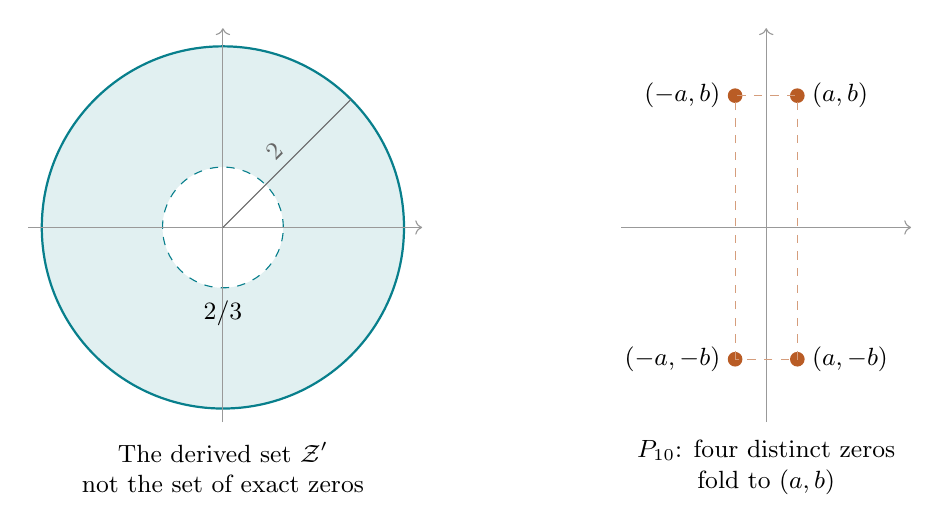
\begin{tikzpicture}[scale=1.15,font=\small]
\begin{scope}[xshift=-3.0cm]
 \fill[accent!12,even odd rule] (0,0) circle(2) (0,0) circle(.666667);
 \draw[accent,thick] (0,0) circle(2);
 \draw[accent,dashed] (0,0) circle(.666667);
 \draw[->,black!40] (-2.15,0)--(2.2,0);
 \draw[->,black!40] (0,-2.15)--(0,2.2);
 \draw[black!60] (0,0)--(1.414214,1.414214)
   node[midway,above,sloped] {$2$};
 \node at (0,-.95) {$2/3$};
 \node[align=center] at (0,-2.65)
 {The derived set $\mathcal Z'$\\not the set of exact zeros};
\end{scope}
\begin{scope}[xshift=3.0cm]
 \draw[->,black!40] (-1.6,0)--(1.6,0);
 \draw[->,black!40] (0,-2.15)--(0,2.2);
 \foreach \x in {-.343561,.343561}
  \foreach \y in {-1.455347,1.455347}
   {\fill[primefive] (\x,\y) circle(2.3pt);}
 \draw[dashed,primefive!60] (-.343561,-1.455347) rectangle(.343561,1.455347);
 \node[right] at (.4,1.455347) {$(a,b)$};
 \node[left] at (-.4,1.455347) {$(-a,b)$};
 \node[right] at (.4,-1.455347) {$(a,-b)$};
 \node[left] at (-.4,-1.455347) {$(-a,-b)$};
 \node[align=center] at (0,-2.65)
 {$P_{10}$: four distinct zeros\\fold to $(a,b)$};
\end{scope}
\end{tikzpicture}
\caption{Two different geometric objects. Left: the exact accumulation
annulus; its inner circle is approached but contains no individual zero.
Right: the four zeros of $z^4+4z^2+5$, a factor of $P_{10}$, with
$a=\sqrt{(\sqrt5-2)/2}$ and $b=\sqrt{(\sqrt5+2)/2}$. The two axis
folds identify this quartet even though the start $10$ is composite.
Coordinates in the drawing are rounded only for plotting.}
\label{C:fig:annulus-and-folds}
\end{figure}

\begin{corollary}[Even composites alone fill the annulus densely]
\label{C:cor:even-composite-annulus}
Let $\mathcal Z_{\mathrm{even,comp}}$ be the union of zeros belonging
to terminating even composite starts. Then
\[
 \mathcal Z_{\mathrm{even,comp}}'
 =\{z:2/3\le|z|\le2\}.
\]
The same conclusion holds if the starts are required to be multiples
of any fixed power $2^h$, $h\ge1$, with finitely many small starts
discarded.
\end{corollary}
\begin{proof}
Take the prefix $v=(0)$, or $v=(0,\ldots,0)$ of length $h$.
All sufficiently large starts supplied by the proof are even and
greater than $2$, hence composite. The proof supplies arbitrarily large
starts, so discarding any finite number of them does not remove the
constructed accumulation points. The reverse inclusion is unchanged.
\end{proof}

\begin{corollary}[Composite density in every prescribed parity class]
\label{C:cor:composite-prefix-annulus}
In Theorem~\ref{C:thm:prefix-annulus}, restricting the starts further to
composite values leaves the derived set unchanged. In particular, odd
composite starts alone have the same derived annulus, even after any
fixed finite initial parity pattern beginning with an odd step is imposed.
\end{corollary}
\begin{proof}
In each fixed-word family used in the theorem, even starts are eventually
composite. For an odd-start family choose a permissible tail length $t_0$
with $N_0=N_{u,t_0}>1$ and let
$D=\operatorname{ord}_{3^R N_0}(2)$. Along $t=t_0+jD$ one has
\[
 2^{L+t}\equiv2^{L+t_0}=3^R N_0+b_u
 \equiv b_u\pmod{3^R N_0},
\]
so $N_{u,t}$ is divisible by $N_0$. For $j\ge1$ it exceeds $N_0$ and
is composite. This subsequence has the same locally uniform polynomial
limit as the full tail family. The two Rouch\'e arguments and the density
conclusion therefore remain valid with composite starts throughout.
\end{proof}

\begin{corollary}[No open geometric region certifies a prime start]
\label{C:cor:no-open-prime-locus}
Every open subset of $\mathbb C$ that meets the closed annulus
$2/3\le|z|\le2$ contains a zero from an even composite start.
Consequently, no nonempty open region inside that annulus, and no open strip
of positive width meeting it, can have the property that every Collatz
zero it contains comes only from a prime start.
\end{corollary}
\begin{proof}
Such an open set contains a nonempty open subset of the open annulus.
Apply Corollary~\ref{C:cor:even-composite-annulus}.
\end{proof}

Corollary~\ref{C:cor:composite-prefix-annulus} gives the same obstruction
when inputs have first been restricted to odd values, or to any one
fixed residue class modulo a power of $2$.

This is a finite-precision obstruction: every neighborhood of a proposed
prime zero in the annulus also admits composite-start zeros. It does not
settle an exact incidence condition on a zero-width line or curve, a test
using algebraic information beyond the location, or a test using the
entire collection of roots of one polynomial. The isolated region
$|z|<2/3$ is also outside this particular no-open-region conclusion.


\begin{corollary}[Arbitrarily narrow approaches to an interior point]
\label{C:cor:ucz-cusps}
Let $2/3<|\zeta|<2$. If $U_j$ are nonempty open subsets of the annulus
with $\sup_{z\in U_j}|z-\zeta|\to0$, then there are distinct Collatz
zeros $\xi_j\in U_j$, after passing to a subsequence if necessary.
In particular, for every $p>0$, zeros approach $1$ through the cusp
\[
 0<|\operatorname{Im}z|,\qquad
 |\operatorname{Re}z-1|<|\operatorname{Im}z|^p.
\]
No nonempty open subset of $2/3<|z|<2$ is free of Collatz zeros.
\end{corollary}
\begin{proof}
Each nonempty open subset of the annulus contains infinitely many
distinct zeros, as proved above. Select a zero avoiding the finitely
many earlier selections. For the cusp, also impose
$0<|z-1|<1/j$; the resulting open set is nonempty for every sufficiently
large $j$.
\end{proof}

This corollary gives a precise interpretation of arbitrary thin
approaches to $1$. It also rules out any proposed universal zero-free
parabolic region whose interior meets the open annulus.


\section{The smallest Collatz zero and finite-degree exclusions}
\label{C:subsec:smallest-collatz-zero}

The inner circle $|z|=2/3$ describes an accumulation boundary, not a
zero-free boundary. In fact, the orbit of $9$ gives
\begin{align*}
P_9(z)={}&9+14z+7z^2+11z^3+17z^4+26z^5+13z^6\\
 &+20z^7+10z^8+5z^9+8z^{10}+4z^{11}+2z^{12}+z^{13}.
\end{align*}
The following result determines the largest open disk centered at the
origin that contains no Collatz zero. It combines an analytic reduction
with an exhaustive certificate using integer arithmetic; it is therefore
explicitly a computer-assisted result.

\begin{theorem}[A unique zero of globally smallest modulus]
\label{C:thm:globally-smallest-zero}
Let $\rho$ be the unique zero of $P_9(-x)$ in
$(13/20,23/35)$. Among all zeros of all terminating Collatz polynomials,
\[
 \min\{|\xi|: P_N(\xi)=0,\ N\ge2,\ \tau(N)<\infty\}=\rho.
\]
Equality is attained only by the pair $(N,\xi)=(9,-\rho)$.
The zero is simple, and $\rho$ is algebraic of degree $13$ over $\mathbb Q$.
Numerically, for orientation only,
\[
 \rho=0.656989767756311659235045725399\ldots.
\]
\end{theorem}

\begin{proof}
Take $r=23/35<2/3$. The finite-cutoff bound
\eqref{C:eq:prefix-finite-cutoff} gives
\[
 P_N(\xi)=0,\quad |\xi|\le23/35
 \quad\Longrightarrow\quad
 N+1\le\frac{4865}{12},\quad\text{hence }N\le404.
\]
Thus an infinite assertion has reduced to $403$ specified starting
values. Every one of their orbits reaches $1$ in at most $91$ steps.
The exact certificate below establishes that $P_9$ has precisely one
zero in $|z|<23/35$, counted with multiplicity, and that every other
$P_N$, $2\le N\le404$, has none in the closed disk.
The same computation establishes that no tested polynomial has a zero
on its boundary.

Direct substitution gives
\[
 P_9(-13/20)=\frac{12282961919783787}{81920000000000000}>0,
 \qquad
 P_9(-23/35)=-\frac{393226451789392713}
 {118272717781982421875}<0.
\]
The intermediate value theorem therefore supplies a negative real zero
in that disk. The count of one proves uniqueness and simplicity. All
other Collatz zeros have modulus greater than $23/35>\rho$, proving the
minimum assertion.

For the degree assertion, reduction modulo $2$ gives
\[
 f(x)=x^{13}+x^9+x^6+x^4+x^3+x^2+1.
\]
It has no linear factor over $\mathbb F_2$, since $f(0)=f(1)=1$.
Repeated squaring gives $x^{2^{13}}\equiv x\pmod f$.
Because $13$ is prime, every irreducible factor of $f$ then has degree
$1$ or $13$; absence of linear factors proves that $f$ is irreducible.
Gauss's lemma proves the irreducibility of $P_9$ over $\mathbb Q$.
The same holds for $P_9(-x)$, proving $[\mathbb Q(\rho):\mathbb Q]=13$.
\end{proof}

\paragraph{Why the disk-count certificate is exact.}
For a real polynomial $F(z)=a_0+\cdots+a_dz^d$ with nonzero constant
and leading coefficients, write
$F^*(z)=z^dF(1/z)$. Suppose $|a_0|>|a_d|$ and put
\[
 Q(z)=a_0F(z)-a_dF^*(z).
\]
The leading term cancels, so $\deg Q<d$, while
$Q(0)=a_0^2-a_d^2\ne0$. If $Q$ has no unit-circle zero, neither does
$F$: a unit-circle zero of a real polynomial is also a zero of its
reciprocal. On the unit circle $|F^*|=|F|$, so Rouch\'e's theorem then
shows that $F$ and $Q$ have the same number of zeros in $|z|<1$.
If $|a_0|<|a_d|$, first replace $F$ by $F^*$; the count for $F$ is
$d$ minus the count for $F^*$. Descending to a nonzero constant proves
both the root count and absence of boundary zeros by induction.
An equality $|a_0|=|a_d|$ would stop this certificate and is explicitly
tested; none occurs in the computation reported here.

To count zeros of $P_N$ in $|z|<23/35$, apply this descent to the
integer polynomial $35^d P_N(23z/35)$. Dividing all coefficients by their
positive greatest common divisor after each transformation changes no
zeros. Thus no rounding, tolerance, numerical root approximation, or
unverified primality test enters the certificate.

\paragraph{Complete in-document verification code.}
The following standard-library Python code is included as part of the
paper; no supplementary source file, package, or data file is required.
It bounds every orbit computation in advance, verifies every strict
comparison, and checks the resulting exact counts. Counts include
multiplicities. The irreducibility check uses binary integers to encode
polynomials over $\mathbb F_2$, with bit $j$ equal to the coefficient of
$x^j$.

\begin{lstlisting}[language=Python]
from math import gcd
from functools import reduce

def orbit(n):
    a = [n]
    for _ in range(91):
        if a[-1] == 1:
            return a
        x = a[-1]
        a.append(x // 2 if x % 2 == 0 else (3*x+1) // 2)
    assert a[-1] == 1
    return a

def count_disk(a):
    count, sign, steps, reversals = 0, 1, 0, 0
    while len(a) > 1:
        while a[-1] == 0:
            a.pop()
        d = len(a) - 1
        if d == 0:
            break
        u, v = a[0], a[-1]
        assert u != 0 and u*u != v*v
        if u*u < v*v:
            a.reverse()
            u, v = v, u
            count += sign*d
            sign = -sign
            reversals += 1
        b = [u*a[j] - v*a[d-j] for j in range(d)]
        g = reduce(gcd, b)
        assert g > 0
        a = [x // g for x in b]
        steps += 1
    assert a[0] != 0
    return count, steps, reversals

rows = []
for n in range(2, 405):
    a = orbit(n)
    d = len(a)-1
    b = [a[j]*23**j*35**(d-j) for j in range(d+1)]
    count, steps, reversals = count_disk(b)
    assert count == (1 if n == 9 else 0)
    assert steps == d
    assert reversals == (1 if n == 9 else 0)
    rows.append((n, d, count, steps, reversals, max(a)))

assert len(rows) == 403
assert max(x[1] for x in rows) == 91
assert sum(x[1] for x in rows) == 13563
assert max(x[5] for x in rows) == 6560
assert sum(x[2] for x in rows) == 1
assert sum(x[3] for x in rows) == 13563
assert sum(x[4] for x in rows) == 1

f = sum(1 << j for j in [13,9,6,4,3,2,0])
u, residues = 2, [2]
for _ in range(13):
    u = sum(((u >> j) & 1) << (2*j)
            for j in range(u.bit_length()))
    while u.bit_length() >= 14:
        u ^= f << (u.bit_length()-14)
    residues.append(u)
assert residues == [2,4,16,256,4840,459,1559,
                    4154,7023,2495,3380,6142,3074,2]
assert u == 2
print("403 orbits; 13563 strict descents; only N=9 has one root")
\end{lstlisting}

The aggregate certificate is:
\[
\begin{array}{c|r|r|r|r}
N\text{ range}&\text{orbits}&\sum\tau(N)&\max\tau(N)
  &\text{zeros in }|z|<23/35\\\hline
2\text{--}99&98&2119&75&1\\
100\text{--}199&100&3521&79&0\\
200\text{--}299&100&3847&81&0\\
300\text{--}404&105&4076&91&0
\end{array}
\]
Only the descent for $N=9$ takes the reciprocal branch, and it does so
once. All other $13562$ comparisons take the direct branch. Every
comparison is strict.

\paragraph{Scope of the conclusion.}
This proves the exact minimum modulus and the complete classification
of zeros in $|z|\le23/35$. It does not claim that $P_9$ supplies the only
zero in the larger disk $|z|<2/3$. The remaining thin band
$23/35<|z|<2/3$ is not classified here. In particular, the accumulation
annulus and the set of actual zeros must still be distinguished.
The result sharpens the universal lower bound $3/5$ obtainable from
Hohertz's orbit-dependent Enestr\"om--Kakeya bound
\cite{R005}. No claim of priority is made without a separate
literature review.

\subsection{A finite-degree exclusion sector near the positive axis}

\begin{proposition}[Degree-dependent separation from $1$]
\label{C:prop:degree-sector}
Let $P_N$ have degree $d=\tau(N)\ge2$. Every zero $\xi$ satisfies
\[
 |\arg\xi|>\frac{\pi}{d},
 \qquad
 |\xi-1|>\sin\!\left(\frac{\pi}{d}\right),
\]
where the argument is taken in $[-\pi,\pi]$. Consequently, if a zero
satisfies $|\xi-1|\le\varepsilon<1$, then
\[
 d>\frac{\pi}{\arcsin\varepsilon}.
\]
\end{proposition}
\begin{proof}
This is an elementary consequence of strictly positive coefficients,
and is not specific to Collatz polynomials. Write $\xi=re^{i\theta}$.
If $|\theta|\le\pi/d$, rotate $P_N(\xi)$ by $e^{-id\theta/2}$.
Every summand has nonnegative real part, and every interior summand
has strictly positive real part. Thus the rotated sum cannot vanish.
The Euclidean distance from $1$ to the complement of the open sector
$|\arg z|<\pi/d$ is $\sin(\pi/d)$; strict angular exclusion gives the
strict distance bound. Finally, monotonicity of sine on $[0,\pi/2]$
gives the degree inequality.
\end{proof}

There is no contradiction with zeros approaching $1$ or with a dense
accumulation annulus: the forbidden sector narrows as the trajectory
length increases. A global forbidden sector of a fixed positive angle
would contradict the annulus theorem; this finite-degree sector does
not. This distinction is particularly important when interpreting a
plot formed from only finitely many starting values.

\subsection{The extremal zero has full symmetric Galois group}

\begin{proposition}[An explicit $S_{13}$ example]
\label{C:prop:extremal-galois}
The Galois group of $P_9$ over $\mathbb Q$ is $S_{13}$.
Consequently, the extremal radius $\rho$ cannot be expressed by radicals
over $\mathbb Q$.
\end{proposition}
\begin{proof}
The preceding irreducibility proof shows that the Galois group $G$
acts transitively on $13$ roots. A transitive group of prime degree is
primitive: all blocks in a block system have equal size dividing $13$.
Modulo $17$, direct multiplication gives
\begin{align*}
P_9(x)\equiv{}&(x+4)(x+5)(x^2+5x-3)\\
&\mathord{}\cdot(x^3+x^2-6x+3)
(x^3+8x^2+x-3)(x^3-4x^2+7x+2).
\end{align*}
The quadratic and the three cubics have no roots in $\mathbb F_{17}$,
as checked by the complete finite calculation below. They are therefore
irreducible over that field. All six monic factors are distinct, so the
reduction is squarefree. By the standard Frobenius--Dedekind theorem
\cite{R075} relating a squarefree factorization modulo a prime to a permutation in
the Galois group, $G$ contains an element of cycle type
$(1,1,2,3,3,3)$. Its cube is a transposition.

For completeness, a primitive permutation group containing a
transposition is the full symmetric group. Form a graph whose edges
are the pairs swapped by all $G$-conjugates of that transposition.
Its connected components form a $G$-invariant block system. Since the
graph has an edge, primitivity makes it connected. Transpositions along
the edges of a connected graph generate the full symmetric group, and
all those transpositions belong to $G$. Thus $G=S_{13}$.
Since $S_{13}$ is not solvable, the irreducible polynomial $P_9(-x)$
is not solvable by radicals; in particular its root $\rho$ is not
expressible by radicals over $\mathbb Q$.
\end{proof}

Here is the complete factorization check, with coefficient lists in
ascending order. It is independent of any computer algebra package.
\begin{lstlisting}[language=Python]
A = [9,14,7,11,17,26,13,20,10,5,8,4,2,1]
factors = [[4,1], [5,1], [-3,5,1], [3,-6,1,1],
           [-3,1,8,1], [2,7,-4,1]]
product = [1]
for a in factors:
    b = [0]*(len(product)+len(a)-1)
    for j, u in enumerate(product):
        for k, v in enumerate(a):
            b[j+k] = (b[j+k]+u*v) % 17
    product = b
assert product == [a % 17 for a in A]
for a in factors[2:]:
    assert all(sum(c*t**j for j,c in enumerate(a)) % 17
               for t in range(17))
assert len({tuple(c % 17 for c in a)
            for a in factors}) == 6
\end{lstlisting}
This determines the Galois group of one explicit extremal polynomial;
it does not purport to classify Galois groups of general Collatz
polynomials, the broader direction raised in
\cite[Section~5, question~6]{R005}.
% Research fragment: exact boundary zeros and a quantitative counting refinement.
% Bibliography needed: Hohertz2022, arXiv:2012.08006v4.
% The classification and block factorization are established results of Hohertz.
% The counting bound below is derived here; no historical-priority claim is made.

\section{Exact boundary zeros and the arithmetic clock}
Throughout this section, $T(n)=n/2$ for even $n$ and
$T(n)=(3n+1)/2$ for odd $n$, and an orbit polynomial stops at its
first visit to $1$. Write $a_j=T^j(N)$, $n=\tau(N)$, and
$P_N(z)=\sum_{j=0}^n a_jz^j$, initially assuming $n<\infty$ and $N>1$.

\subsection{The established boundary classification, with a direct proof}
The following classification is Hohertz's Theorem III
\cite{R005}. We include a short proof using a coefficient identity,
both to make the mechanism explicit and to distinguish this known theorem
from the quantitative estimate proved below.

\begin{theorem}[Hohertz's boundary classification]\label{C:thm:boundary-known}
Define
\[
 d_N=\gcd\bigl(\{n+1\}\cup
     \{j+1:0\le j<n,\ a_j\text{ odd}\}\bigr).
\]
The zeros of $P_N$ on $|z|=2$ are precisely
\[
 \bigl\{2\omega:\omega^{d_N}=1,\ \omega\ne1\bigr\}.
\]
There are $d_N-1$ such zeros, all simple. Every other zero has modulus
strictly less than $2$.
\end{theorem}

\begin{proof}
Direct subtraction of coefficients gives the defect identity
\begin{equation}\label{C:eq:boundary-defect}
 (z-2)P_N(z)=z^{n+1}-2N-
 \sum_{\substack{0\le j<n\\a_j\text{ odd}}}(2a_j+1)z^{j+1}.
\end{equation}
Indeed, the coefficient of $z^{j+1}$ in the left side is
$a_j-2a_{j+1}$, which is $0$ for even $a_j$ and $-(2a_j+1)$
for odd $a_j$. Evaluating at $z=2$ yields
\[
 2^{n+1}=2N+
 \sum_{\substack{0\le j<n\\a_j\text{ odd}}}(2a_j+1)2^{j+1}.
\]
For a zero $z=2\omega$, $|\omega|=1$, equality in the triangle
inequality in \eqref{C:eq:boundary-defect} forces
\[
 \omega^{n+1}=1,\qquad
 \omega^{j+1}=1\quad\text{for every odd }a_j, j<n,
\]
because the constant term $2N$ on the right is positive.
These conditions are equivalent to $\omega^{d_N}=1$ and conversely
make the right side of \eqref{C:eq:boundary-defect} vanish.
The value $z=2$ must be discarded because $P_N(2)>0$.

Put $G(z)=(z-2)P_N(z)$. At any of the displayed roots of $G$,
\[
 zG'(z)=(n+1)2^{n+1}
 -\sum_{\substack{0\le j<n\\a_j\text{ odd}}}
 (j+1)(2a_j+1)2^{j+1}>0.
\]
The last inequality follows from the preceding identity and $j+1<n+1$.
Thus these roots are simple. Finally, the positive-coefficient
Enestr\"om--Kakeya bound gives $|z|\le2$ for all zeros, since
$a_j/a_{j+1}\le2$. Equivalently, the same upper bound follows from
\eqref{C:eq:boundary-defect}: for $r>2$, dividing by $r^{n+1}$ makes
every term on its right smaller than its value at $r=2$.
\end{proof}

Hohertz uses the equivalent gcd of $n+1$ and the integers $n-j$ at
odd positions. The two forms agree because $(n+1)-(j+1)=n-j$.

\subsection{A valuation formula and prime starting values}
Write $e=v_2(N)$. Remove the initial divisions by $2$, and denote the
subsequent odd values by
\[
 u_0=N/2^e,\ u_1,\ldots,u_\ell=1,
 \qquad k_i=v_2(3u_i+1),\quad
 u_{i+1}=(3u_i+1)/2^{k_i}.
\]
When $N$ is a power of $2$, take $\ell=0$ and $u_0=1$.

\begin{proposition}[The arithmetic clock]\label{C:prop:boundary-clock}
With the preceding convention,
\[
 \boxed{d_N=\gcd(e+1,k_0,\ldots,k_{\ell-1}).}
\]
In particular $d_N\mid e+1$, and the number of boundary zeros is at most
$v_2(N)$.
\end{proposition}

\begin{proof}
The odd positions are $j_0=e$ and
$j_{i+1}=j_i+k_i$, with $j_\ell=n$. The gcd in
Theorem~\ref{C:thm:boundary-known} is the gcd of
$j_0+1,\ldots,j_\ell+1$, hence the gcd of $e+1$ and their successive
differences $k_i$. In the power-of-$2$ case it is simply $e+1$.
\end{proof}

\begin{corollary}[Prime starts cannot hit the outer circle]
Every terminating odd starting value, prime or composite, has $d_N=1$.
Consequently all zeros of $P_p$ have $|z|<2$ for every odd prime $p$
whose orbit terminates. The sole prime exception is $p=2$, for which
$P_2(z)=2+z$ has the zero $-2$.
\end{corollary}

This is a parity restriction, not a primality criterion. In particular,
the absence of outer-boundary zeros cannot distinguish odd primes from
odd composite integers.

\begin{proposition}[An unconditional terminating decision procedure]
There is a finite procedure, independent of the general Collatz conjecture,
which decides whether a positive integer belongs to the set of terminating
starts having an outer-boundary zero.
\end{proposition}

\begin{proof}
For $N>1$, start with $g=v_2(N)+1$ and $u=N/2^{v_2(N)}$.
If $g=1$, answer no. While $u>1$ and $g>1$, set
$k=v_2(3u+1)$ and replace $g$ by $\gcd(g,k)$.
If this makes $g=1$, answer no immediately; otherwise replace
$u$ by $(3u+1)/2^k$ and continue. Every such continuation has
$k\ge2$, and therefore $1\le(3u+1)/2^k<u$ for $u>1$.
Thus the procedure stops. If it reaches $u=1$ with $g>1$, its explicitly
constructed orbit terminates and Proposition~\ref{C:prop:boundary-clock}
gives $d_N=g>1$. Conversely, if a gcd ever becomes $1$, every later gcd
stays $1$, so a terminating orbit cannot have a boundary zero.
For $N=1$, the polynomial is constant and the answer is no.
\end{proof}

\subsection{Integral factorization and exact two-circle examples}
The block factorization below is the integral-variable version of
Hohertz's factorization, not a new boundary classification.

\begin{proposition}[Block factorization]\label{C:prop:boundary-block}
Set $d=d_N$ and
\[
 B_d(z)=\frac{z^d-2^d}{z-2}
       =\sum_{j=0}^{d-1}2^{d-1-j}z^j.
\]
Then
\[
 P_N(z)=B_d(z)Q_N(z^d),
 \qquad Q_N\in\mathbb Z_{>0}[w],
\]
where $Q_N$ is monic. If $m=(n+1)/d-1$, explicitly
\[
 Q_N(w)=\sum_{t=0}^{m}a_{dt+d-1}w^t.
\]
All roots of $Q_N$ have modulus strictly less than $2^d$.
The largest order of rotational invariance of the polynomial
$(z-2)P_N(z)$ is exactly $d$.
\end{proposition}

\begin{proof}
All odd positions satisfy $j\equiv d-1\pmod d$. Thus within each
block of $d$ coefficients,
$a_{dt+j}=2^{d-1-j}a_{dt+d-1}$ for $0\le j<d$.
This gives the factorization and positive integral coefficients; the
last block ends in $a_n=1$, so $Q_N$ is monic. Its root bound follows
from Theorem~\ref{C:thm:boundary-known}, since $B_d$ already accounts for
all boundary zeros. Finally, the nonconstant support exponents in
\eqref{C:eq:boundary-defect} have gcd $d$. Hence
$G(\omega z)=G(z)$ holds for all $z$ exactly when $\omega^d=1$.
\end{proof}

\begin{proposition}[An explicit family of two regular polygons]
For every even integer $d\ge4$, set
\[
 q=\frac{2^d-1}{3},\qquad N=2^{d-1}q.
\]
Then
\[
 \boxed{P_N(z)=\frac{z^d-2^d}{z-2}(z^d+q).}
\]
Its zeros consist of $d-1$ points on the outer circle and $d$ points
on an inner circle:
\[
 2e^{2\pi i j/d}\ (1\le j<d),\qquad
 q^{1/d}e^{(2j+1)\pi i/d}\ (0\le j<d).
\]
The inner radii satisfy $q^{1/d}<2$ and tend to $2$ as $d\to\infty$.
Within this family, $q$ is prime if and only if $d=4$.
\end{proposition}

\begin{proof}
The orbit begins with $2^{d-1}q,\ldots,q$, and because $3q+1=2^d$
it continues with $2^{d-1},\ldots,1$. These are two blocks of $d$
coefficients, giving the formula. The root locations follow by solving
the two factors. For the final assertion write $d=2h$. Then
\[
 q=\frac{(2^h-1)(2^h+1)}3.
\]
Exactly one factor is divisible by $3$. If $h\ge3$, both factors
remain greater than $1$ after this division; when $h=2$, the result
is $q=5$.
\end{proof}

For example,
\[
 P_{40}(z)=(z^3+2z^2+4z+8)(z^4+5).
\]
The three outer zeros are $-2,2i,-2i$; the other four form a square
of radius $5^{1/4}$. The inner factor is irreducible over $\mathbb Q$
by Eisenstein's criterion at $5$. This is an exact arithmetic explanation
of one visually distinctive pattern in a root plot.


\begin{figure}[htbp]
\centering
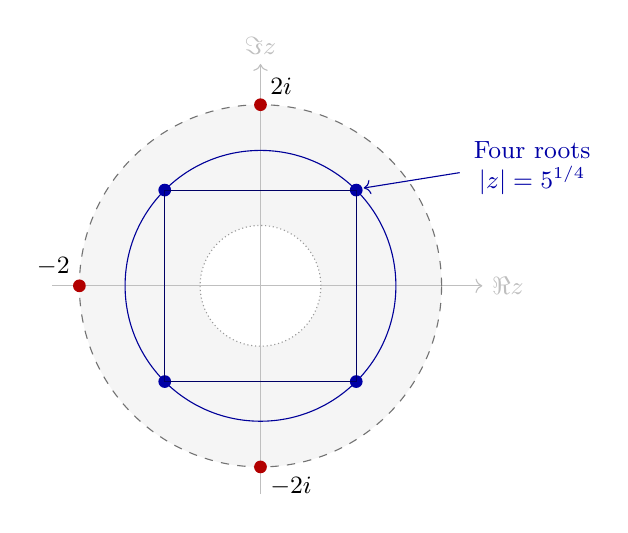
\begin{tikzpicture}[scale=1.15,font=\small]
\fill[black!4] (0,0) circle (2);
\fill[white] (0,0) circle (0.6666667);
\draw[black!25,->] (-2.3,0)--(2.45,0) node[right] {$\Re z$};
\draw[black!25,->] (0,-2.3)--(0,2.45) node[above] {$\Im z$};
\draw[dashed,black!55] (0,0) circle (2);
\draw[densely dotted,black!40] (0,0) circle (0.6666667);
\draw[blue!60!black] (0,0) circle (1.495349);
\foreach \a in {45,135,225,315}{\fill[blue!65!black] (\a:1.495349) circle (2pt);}
\draw[blue!40!black] (45:1.495349)--(135:1.495349)--(225:1.495349)--(315:1.495349)--cycle;
\foreach \a in {90,180,270}{\fill[red!70!black] (\a:2) circle (2pt);}
\node[above left] at (-2,0) {$-2$};
\node[above right] at (0,2) {$2i$};
\node[below right] at (0,-2) {$-2i$};
\node[blue!65!black,align=center] at (3,1.3) {Four roots\\$|z|=5^{1/4}$};
\draw[blue!60!black,->] (2.2,1.25)--(1.14,1.08);
\end{tikzpicture}
\caption{Exact zeros of $P_{40}$. The outer geometric factor contributes
three points; the irreducible factor $z^4+5$ contributes a rotated square.
The dotted inner circle $|z|=2/3$ is shown only as a reference.}
\end{figure}
\subsection{A quantitative bound for boundary starts}
Hohertz proves that the set of starting integers with outer-boundary zeros
has natural density zero. The next argument gives a stronger explicit bound.
We make no claim here that the bound has not appeared elsewhere.

\begin{lemma}[Finite parity prefixes]\label{C:lem:boundary-parity}
For the shortcut map, each prescribed parity word of length $k$ corresponds
to exactly one residue class of starting integers modulo $2^k$.
\end{lemma}

\begin{proof}
After a fixed prefix with $r$ odd branches, the iterate is
$(3^rN+b)/2^k$ for an integer $b$. Inductively, a length-$k$ prefix
specifies one class modulo $2^k$. Its two lifts modulo $2^{k+1}$
differ by $2^k$ in the input and by the odd integer $3^r$ in the
$k$th iterate, so exactly one lift has either prescribed next parity.
The length-zero case starts the induction.
\end{proof}

\begin{theorem}[A square-root upper bound]\label{C:thm:boundary-sqrt}
For $X\ge4$, put $k=\lfloor\log_2X\rfloor$ and
\[
 A_d(X)=\#\{2\le N\le X:\tau(N)<\infty,\ d\mid d_N\},
 \qquad d\ge2.
\]
Then
\[
 A_d(X)\le3\,2^{\lfloor k/d\rfloor}-1.
\]
Consequently, if $E(X)$ counts the starts $2\le N\le X$ whose
terminating orbit polynomials have a zero on $|z|=2$, then
\[
 \boxed{
 E(X)\le3\,2^{\lfloor k/2\rfloor}
       +3(k-1)2^{\lfloor k/3\rfloor}
       =O(\sqrt X).}
\]
In particular, $E(X)\le(3+o(1))\sqrt X$. No global convergence
assumption is used.
\end{theorem}

\begin{proof}
If $d\mid d_N$, odd positions before the terminal $1$ must lie at
$j\equiv d-1\pmod d$, and $n+1$ must be divisible by $d$.
First count starts with $n\ge k$. Among their first $k$ parity bits,
only $\lfloor k/d\rfloor$ positions can be odd. There are at most
$2^{\lfloor k/d\rfloor}$ such words. By
Lemma~\ref{C:lem:boundary-parity}, each is one residue class modulo $2^k$;
because $2^k\le X<2^{k+1}$, each class supplies at most two starts.
This part contributes at most $2\cdot2^{\lfloor k/d\rfloor}$.

For the starts with $n<k$, write $n=dq-1$, where
$1\le q\le\lfloor k/d\rfloor$. Only the $q-1$ positions
$d-1,2d-1,\ldots,(q-1)d-1$ can be odd before time $n$.
There are at most $2^{q-1}$ words. A complete parity word and the
terminal value $1$ determine at most one starting value, because each
branch is an injective affine map. Summing over $q$ gives at most
$2^{\lfloor k/d\rfloor}-1$, proving the first estimate.

If $d_N>1$, then $2\le d_N\le v_2(N)+1\le k+1$.
Take the union over $d=2,\ldots,k+1$, separate the term $d=2$,
and use $\lfloor k/d\rfloor\le\lfloor k/3\rfloor$ for the other
$k-1$ terms. This gives the displayed bound. Finally,
$kX^{1/3}=o(X^{1/2})$.
\end{proof}

The exponent $1/2$ is an upper bound, not an established optimal exponent
or an asymptotic formula. Determining the actual growth of $E(X)$ remains
a concrete counting problem. These facts explain algebraic patterns and
rarity on the outer circle; they do not identify Collatz zeros with zeta
zeros or imply a statement about the Riemann hypothesis.

% Suggested bibliography:
% \bibitem{Hohertz2022} M. Hohertz,
% Bounds for zeros of Collatz polynomials, with necessary and sufficient
% strictness conditions, arXiv:2012.08006v4 (2022),
% https://arxiv.org/abs/2012.08006 .

\subsection{A positive power lower bound from an inverse tree}
The previous upper bound leaves open how many starts actually produce
boundary zeros. A complementary lower bound follows from an explicit
terminating inverse tree. This is an additional deduction of the present
compilation; no claim of historical priority is made.

\begin{theorem}[Polynomially many starts with the boundary zero $-2$]
\label{C:thm:boundary-power-lower}
For $B\ge2$, let $s_B>0$ be the unique solution of
\[
 \sum_{j=1}^{B}\left(\frac{3}{64^j}\right)^{s_B}=1.
\]
Let $E(X)$ count terminating starts $2\le N\le X$ whose polynomials
have a zero on $|z|=2$. For every $X\ge170$,
\[
 E(X)>\frac{(X/170)^{s_B}-1}{B-1}.
\]
Every start constructed in this proof has $d_N=2$, so its only
outer-boundary zero is $-2$. In particular,
\begin{equation}\label{C:eq:boundary-exponent-bracket}
 s_*\le\liminf_{X\to\infty}\frac{\log E(X)}{\log X}
 \le\limsup_{X\to\infty}\frac{\log E(X)}{\log X}\le\frac12,
 \qquad 64^{s_*}=1+3^{s_*},
\end{equation}
where $s_*=0.1935935685\ldots$. For example,
$s_2=0.1433841276\ldots$.
\end{theorem}
\begin{proof}
Use the accelerated odd map
$U(v)=(3v+1)/2^{v_2(3v+1)}$. Start the inverse tree at $v=85$;
then $U(85)=1$ and $v_2(3\cdot85+1)=8$.
For every odd $v\equiv1\pmod3$, exactly one
$a_0\in\{1,2,3\}$ satisfies
\[
 4^{a_0}v\equiv4\pmod9.
\]
Indeed, $v\bmod9$ belongs to $\{1,4,7\}$, and multiplication by $4$
cycles these three residues. For $j=1,\ldots,B$, define the children
\[
 v_j=\frac{4^{a_0+3(j-1)}v-1}{3}.
\]
Each child is an odd integer congruent to $1$ modulo $3$, and
\[
 U(v_j)=v,\qquad
 v_2(3v_j+1)=2a_0+6(j-1),\qquad
 v<v_j< c_jv,\quad c_j=64^j/3.
\]
The strict growth uses $v\ge85$.
Every node therefore has a terminating orbit, with all accelerated
valuation exponents even. Distinct children have different valuation
exponents, so are different; a node has its unique parent under $U$.
Strict growth rules out cycles. If two nodes at different depths were
equal, applying their common unique successive parents would make a
positive iterate of $85$ return to $85$, whereas its first successor
is $1$. Thus every word in the child indices gives a distinct node.

For a word $w=(j_1,\ldots,j_k)$ put
$C(w)=\prod_{i=1}^k c_{j_i}$, with $C(\varnothing)=1$.
Its node obeys $v(w)\le85C(w)$, so the even start
$N(w)=2v(w)$ obeys $N(w)\le170C(w)$.
Its initial $2$-adic valuation is $1$, and every following odd-step
valuation is even; hence the arithmetic clock gives
\[
 d_{N(w)}=\gcd(2,\hbox{the following even valuations})=2.
\]
It remains to count words with $C(w)\le Y=X/170$.

Stop a word at the first time $C(w)>Y$. Since every $c_j>1$,
this produces a finite full $B$-ary tree. Its internal nodes are exactly
the words with $C(w)\le Y$; all of them give counted starts.
Assign a child of index $j$ the relative mass $c_j^{-s_B}$.
These masses sum to $1$, so the sum of the leaf masses
$C(w)^{-s_B}$ is $1$. Every leaf has $C(w)>Y$, and hence has
mass less than $Y^{-s_B}$. If $L$ is the number of leaves, then
$L>Y^{s_B}$. A finite full $B$-ary tree has $(L-1)/(B-1)$ internal
nodes. Consequently
\[
 E(X)\ge\frac{L-1}{B-1}>\frac{Y^{s_B}-1}{B-1}.
\]

As $B$ increases, $s_B$ increases to the unique positive solution of
\[
 \sum_{j=1}^{\infty}(3/64^j)^s
 =\frac{3^s}{64^s-1}=1,
\]
which is $s_*$. For every fixed $B$ the lower bound implies
$\liminf\log E(X)/\log X\ge s_B$; taking the supremum over $B$
gives the left side of \eqref{C:eq:boundary-exponent-bracket}.
The square-root upper bound gives the right side.
\end{proof}

The interval of possible growth exponents is narrower, but neither
an exact exponent nor a full asymptotic for $E(X)$ is proved.

\section{Zero-cloud measures and the frequency of odd Collatz steps}
\label{C:sec:zd-distribution}

Topological accumulation describes where a zero can be found arbitrarily
nearby. It does not describe the proportion of all zeros in a region.
The distinction is substantial for Collatz polynomials. The results in this
section are elementary deductions from their coefficient structure and the
finite-word construction; no assertion of historical priority is made.

Let $N>1$ reach $1$ under the shortcut map $T$, set
$a_j=T^j(N)$, $\tau=\min\{j:a_j=1\}$, and write
\[
 P_N(z)=\sum_{j=0}^{\tau}a_jz^j
       =\prod_{\nu=1}^{\tau}(z-\zeta_\nu).
\]
Zeros are counted with algebraic multiplicity. Define
\[
 r_N=\#\{0\le j<\tau:a_j\text{ is odd}\},\qquad
 \mu_N=\frac1\tau\sum_{\nu=1}^{\tau}\delta_{\zeta_\nu}.
\]

\begin{theorem}[Exact logarithmic radius and a small error term]
\label{C:thm:zd-radius-clock}
Put
\[
 E_N=\sum_{\substack{0\le j<\tau\\a_j\text{ odd}}}
        \log\left(1+\frac1{3a_j}\right).
\]
Then
\begin{align}
 \log N&=\tau\log2-r_N\log3-E_N,
 \label{C:eq:zd-clock}\\
 0\le E_N&\le\frac16\log(2r_N+1),
 \label{C:eq:zd-error}\\
 \left(\prod_{\nu=1}^{\tau}|\zeta_\nu|\right)^{1/\tau}
 &=N^{1/\tau}
 =2\,3^{-r_N/\tau}e^{-E_N/\tau}.
 \label{C:eq:zd-geometric-mean}
\end{align}
In particular, $r_N/\tau<\log2/\log3$.
\end{theorem}
\begin{proof}
On an even step $a_{j+1}/a_j=1/2$, and on an odd step
$a_{j+1}/a_j=(3/2)(1+1/(3a_j))$. Multiplying these identities from
$j=0$ to $\tau-1$, with $a_\tau=1$, gives
\eqref{C:eq:zd-clock}. A terminating orbit cannot repeat a value before
its first $1$, since a repeat would trap it in a cycle. Its odd values
before that time are therefore distinct integers at least $3$.
If ordered increasingly as $u_1<\cdots<u_R$, they satisfy $u_i\ge2i+1$.
For $R\ge1$, using $\log(1+x)\le x$ gives
\[
 E_N\le\frac13\sum_{i=1}^R\frac1{2i+1}
 \le\frac13\int_0^R\frac{dx}{2x+1}
 =\frac16\log(2R+1).
\]
For $R=0$, both sides are zero. The monic polynomial has constant term
$N$, so Vieta's formula gives $\prod|\zeta_\nu|=N$, proving
\eqref{C:eq:zd-geometric-mean}. Finally, $\log N>0$ and $E_N\ge0$ in
\eqref{C:eq:zd-clock} give the strict bound on $r_N/\tau$.
\end{proof}

This identifies an arithmetic feature of the orbit inside the zero cloud:
the average logarithmic radius determines the proportion of odd steps up
to an error $O(\log\tau/\tau)$. It concerns ordinary odd steps of the
shortcut map, not the number of prime values visited.

\begin{proposition}[Exact terminal moments and universal moment bounds]
\label{C:prop:zd-moments}
For every integer $k\ge1$, the real power sums satisfy
\[
 -2^k\le\sum_{\nu=1}^{\tau}\zeta_\nu^k\le(k-1)2^k.
\]
If $\tau\ge3$, then
\[
 \sum_\nu\zeta_\nu=-2,\qquad
 \sum_\nu\zeta_\nu^2=-4,\qquad
 \sum_\nu\zeta_\nu^3=-8.
\]
If $\tau\ge4$, then
\[
 \sum_\nu\zeta_\nu^4
 =48-4a_{\tau-4}
 =\begin{cases}-16,&a_{\tau-4}=16,\\28,&a_{\tau-4}=5.
 \end{cases}
\]
\end{proposition}
\begin{proof}
Every inverse step satisfies $a_j\le2a_{j+1}$. Therefore
$c_j=2^{-j}a_{\tau-j}$ decreases from $c_0=1$ to $c_\tau>0$.
For $w_\nu=\zeta_\nu/2$, the reversed normalized polynomial is
\[
 F(u)=\sum_{j=0}^{\tau}c_ju^j
     =\prod_{\nu=1}^{\tau}(1-w_\nu u).
\]
Put $d_j=c_{j-1}-c_j$ for $1\le j\le\tau$ and
$d_{\tau+1}=c_\tau$. Then $d_j\ge0$, $\sum d_j=1$, and
\[
 (1-u)F(u)=1-D(u),\qquad D(u)=\sum_{j=1}^{\tau+1}d_ju^j.
\]
Comparing coefficients in the formal logarithms gives
\[
 S_k:=\sum_\nu w_\nu^k
 =-1+k\sum_{m\ge1}\frac1m[u^k]D(u)^m.
\]
Every coefficient on the right is nonnegative, proving $S_k\ge-1$.
Write $(1-D(u))^{-1}=\sum_{n\ge0}v_nu^n$. The recurrence
$v_0=1$ and $v_n=\sum_{j=1}^{n}d_jv_{n-j}$, with $d_j=0$
beyond its defined range, shows by induction that $0\le v_n\le1$.
Consequently, for $k\ge1$,
\[
 \sum_{m\ge1}\frac1m[u^k]D(u)^m
 \le\sum_{m\ge1}[u^k]D(u)^m=v_k\le1.
\]
Thus $S_k\le k-1$, and multiplication by $2^k$ proves the bound.
This argument also shows that the sums are real; alternatively,
nonreal roots occur in conjugate pairs.

The final three predecessors of a first visit to $1$ are necessarily
$8,4,2$ whenever they exist. The next predecessor is either $16$ or
$5$. Substitution into Newton's identities in the original variable
gives the displayed exact sums. The lower bound is sharp, and the upper bound is sharp for $k\ge2$, across
the family: for $N=2^t$, $S_k=-1$ when $(t+1)\nmid k$, and
$S_{t+1}=t$.
\end{proof}

\begin{theorem}[Constraints on every limiting full zero cloud]
\label{C:thm:zd-limit-constraints}
Let $N_j\to\infty$ be terminating starting values, and suppose
$\mu_{N_j}$ converges weakly to a probability measure $\mu$.
Then
\begin{enumerate}
\item $\mu$ is supported on $2/3\le|z|\le2$;
\item $\int z^k\,d\mu(z)=0$ for every integer $k\ge1$;
\item $0\le\int\log|z|\,d\mu(z)\le\log2$, and
\[
 \frac{r_{N_j}}{\tau(N_j)}\longrightarrow
 \frac{\log2-\int\log|z|\,d\mu(z)}{\log3};
\]
\item for every point $z_0$ in the support,
\[
 \mu(\{z_0\})\le\frac{2-|z_0|}{2+|z_0|}.
\]
In particular, there are no atoms on $|z|=2$, and the possible mass at
$z=1$ is at most $1/3$.
\end{enumerate}
\end{theorem}
\begin{proof}
The coefficient bound $N\le2^\tau$ implies $\tau(N_j)\to\infty$.
The outer radius bound $|\zeta|\le2$ and the initial-value lower bound
tending to $2/3$ give the asserted support. Proposition
\ref{C:prop:zd-moments}, divided by $\tau(N_j)$, proves the vanishing
analytic moments. Since all sufficiently late zero clouds stay away
from zero, weak convergence also gives
\[
 \int\log|z|\,d\mu(z)
 =\lim_j\frac{\log N_j}{\tau(N_j)}\in[0,\log2].
\]
Equation~\eqref{C:eq:zd-clock} and
$E_{N_j}/\tau(N_j)=O(\log\tau(N_j)/\tau(N_j))$ then prove the
odd-step frequency formula.

For the atom bound, scale $w=z/2$ and write $w_0=re^{i\theta}$.
For $0<t<1$, the function
\[
 H_t(w)=\operatorname{Re}
       \frac{1+te^{-i\theta}w}{1-te^{-i\theta}w}
\]
is positive on the closed unit disk. Its uniformly convergent power
series and the vanishing analytic moments give $\int H_t\,d\mu=1$
(with the scaling understood). At $w_0$ its value is
$(1+tr)/(1-tr)$. Hence
$\mu(\{z_0\})\le(1-tr)/(1+tr)$; let $t\uparrow1$.
\end{proof}

One consequence is that the full zero cloud cannot converge to a
probability measure carried by a circle of radius strictly smaller than
$1$. Such a measure would have negative average $\log|z|$. Nevertheless,
individual zeros accumulate on every such circle between $2/3$ and $1$.
The topological annulus theorem and this statistical restriction are
compatible because individual exceptional zeros may carry vanishing
mass in $\mu_N$.

\begin{theorem}[Outer-circle equidistribution for sparse odd steps]
\label{C:thm:zd-outer-equidistribution}
If $N_j\to\infty$ are terminating starts and
$r_{N_j}=o(\tau(N_j))$, then $\mu_{N_j}$ converges to normalized
arclength on $|z|=2$.
For every $0<r<2$, the following quantitative radial bound holds:
\[
 \#\{\nu:|\zeta_\nu|\le r\}
 \le\frac{\tau\log2-\log N}{\log(2/r)}
 =\frac{r_N\log3+E_N}{\log(2/r)}.
\]
\end{theorem}
\begin{proof}
Every zero has modulus at most $2$, and Vieta's formula gives
\[
 \sum_\nu\log\frac2{|\zeta_\nu|}
 =\tau\log2-\log N.
\]
Each zero in $|z|\le r$ contributes at least $\log(2/r)$, proving
the bound. Its right side is $o(\tau)$ under the stated hypothesis.
Every weakly convergent subsequence is therefore supported on $|z|=2$.
Its analytic moments vanish by Proposition~\ref{C:prop:zd-moments}.
After scaling to the unit circle, all positive Fourier coefficients
vanish; the negative coefficients are their complex conjugates.
Uniqueness of a probability measure from its Fourier coefficients
identifies the limit as normalized arclength. Compactness of probability
measures on $|z|\le2$ then proves convergence of the entire sequence.
\end{proof}

For example, $N=2^t$ has $r_N=0$ and
\[
 P_{2^t}(z)=2^t\sum_{j=0}^t(z/2)^j.
\]
Its roots are exactly $2\exp(2\pi i k/(t+1))$, $1\le k\le t$,
which visibly become uniformly spaced on the outer circle. The theorem
allows an unbounded number of odd steps as long as their proportion
tends to zero.

There is also a concrete family with an exact interior zero. For odd
$t\ge3$, put $N_t=(2^{t+1}-1)/3$. Its orbit is
$N_t,2^t,2^{t-1},\ldots,1$, so it has exactly one odd step and degree
$t+1$. An alternating geometric sum gives
\[
 P_{N_t}(-1)=\frac{2^{t+1}-1}{3}
             +\sum_{j=1}^{t+1}2^{t+1-j}(-1)^j=0.
\]
Moreover, $P_{N_t}^{\prime}(-1)=(2N_t-t-1)/3>0$, so this zero is simple.
Thus the starts $5,21,85,341,\ldots$ retain the exact zero $-1$,
while their full zero-cloud measures converge to uniform arclength on
$|z|=2$. The one interior root has normalized mass $1/(t+1)$,
which tends to zero.

\begin{corollary}[Dense selected zeros with all statistical mass at the rim]
\label{C:cor:zd-density-versus-mass}
Let $U_1,U_2,\ldots$ be nonempty open sets, each meeting the open
annulus $2/3<|z|<2$. There are terminating starts $N_j\to\infty$
and zeros $\xi_j$ of $P_{N_j}$ such that
\[
 \xi_j\in U_j,\qquad
 \mu_{N_j}\Longrightarrow\text{normalized arclength on }|z|=2.
\]
In particular, the selected zeros may be dense throughout the entire
annulus while the normalized full zero clouds converge to its outer rim.
\end{corollary}
\begin{proof}
The repeated-word proof of the annulus theorem has a useful feature:
for each open set $U_j$ one can first fix a finite parity prefix so that
its power-of-two-tail limit has a zero in $U_j$, and then let the tail
length $t$ tend to infinity through an arithmetic progression.
Rouch\'e's theorem supplies a zero in $U_j$ for all sufficiently large
permitted $t$. The prefix length and its odd-step count are fixed during
this last limit, whereas the total length is the prefix length plus $t$.
Choose $t$ large enough that $r_{N_j}/\tau(N_j)<1/j$ and $N_j>j$.
The preceding theorem gives the claimed convergence. To obtain density,
choose the $U_j$ from a countable base of open disks meeting the annulus,
repeating each such disk infinitely often.
\end{proof}

The distribution results do not assume that all positive integers, or all
primes, terminate. They do not assert a universal statistical distribution
when the odd-step proportion stays positive.
% Standalone section fragment. Uses the theorem environments of the parent paper.
% Bibliography entry needed: HohertzKalantari2020, arXiv:2001.00482v2.

\section{Exact vertical lines and a composite imaginary-axis family}

All statements below concern positive starting integers $N>1$ whose shortcut Collatz
orbit reaches $1$. Write
\[
 P_N(z)=\sum_{j=0}^{L}a_jz^j,\qquad a_0=N,\quad a_L=1,
\]
where $L$ is the first hitting time of $1$. Thus $P_N$ is monic with integer
coefficients. We use the established bound $|\alpha|\leq2$ for its zeros.

\begin{proposition}[Rational vertical lines]
If a nonreal zero $\alpha$ of $P_N$ has rational real part, then
$k=2\operatorname{Re}\alpha$ is an integer. Its monic minimal polynomial has
even degree and has the form
\[
 f(z)=g(z^2-kz),\qquad g\in\mathbb Z[z].
\]
In particular, the only rational-real-part vertical lines on which a nonreal
zero can lie are
\[
 \operatorname{Re}z\in
 \left\{-\frac32,-1,-\frac12,0,\frac12,1,\frac32\right\}.
\]
If $N$ is odd and $c=f(0)$, then $\gcd(c,k)=1$.
\end{proposition}
\begin{proof}
The sum $\alpha+\overline\alpha$ is a rational algebraic integer, so it is an
integer $k$. Complex conjugation and minimality give
$f(k-z)=(-1)^df(z)$, where $d=\deg f$. If $d$ were odd, substituting $z=k/2$
would give a rational zero of $f$, contradicting irreducibility and the
nonreality of $\alpha$. Hence $d$ is even and $f(k-z)=f(z)$.
Every integral polynomial invariant under $z\mapsto k-z$ belongs to
$\mathbb Z[z^2-kz]$: subtract its leading coefficient times
$(z^2-kz)^{d/2}$ and proceed by induction on the degree. The radius bound
and nonreality imply $|k|<4$, proving the displayed list.

Since $f$ is monic, division in $\mathbb Z[z]$ gives $P_N=fh$ for some
$h\in\mathbb Z[z]$. A prime dividing both $f(0)$ and $f'(0)$ would divide
both $P_N(0)$ and $P_N'(0)$. For odd $N$ these two integers are
$N$ and $(3N+1)/2$, which are coprime. Thus
$\gcd(f(0),f'(0))=1$. Since $f'(0)=-k g'(0)$, we obtain
$\gcd(c,k)=1$.
\end{proof}

\begin{corollary}[Imaginary roots of odd starts are units]
For every odd starting integer $N$, any purely imaginary zero of $P_N$ is
an algebraic unit. More generally, every even monic integral factor of
$P_N$ has constant coefficient $\pm1$.
\end{corollary}
\begin{proof}
An even factor $f$ satisfies $f'(0)=0$. If $P_N=fh$, then $f(0)$ divides
both $P_N(0)=N$ and $P_N'(0)=(3N+1)/2$, whose gcd is $1$.
For a purely imaginary zero, its minimal polynomial is even by the
preceding proposition with $k=0$.
\end{proof}

This is a restriction on all odd starts, including odd composites; it is not
a primality criterion. In particular, if $p$ is an odd prime and $G_p$ is
the unique irreducible factor of $P_p$ with constant coefficient of absolute
value $p$, then $G_p$ has no imaginary-axis zero. Possible zeros of
unit-constant factors are not excluded by this argument.

\begin{proposition}[Infinitely many composite starts on the imaginary axis]
For every integer $r\geq0$, put $N_r=42\cdot16^r$. The polynomial $P_{N_r}$
has exactly one conjugate pair of imaginary-axis zeros. They are
\[
 \alpha_r^\pm=\pm i\sqrt{x_r},
\]
where $x_r$ is the unique positive solution of
\[
 x_r^{2r+1}(43+x_r^3)=84\cdot16^r.
\]
Moreover $0<x_r<4$, $x_r$ increases strictly with $r$, and $x_r\longrightarrow4$.
Consequently $\alpha_r^\pm\longrightarrow\pm2i$ from the interior of the
radius-two disk. Every $N_r$ is composite.
\end{proposition}
\begin{proof}
More generally let $N=42\cdot4^u=21\cdot2^{2u+1}$, with $u\geq0$.
After $2u+1$ halvings the orbit reaches $21$, followed by
$32,16,8,4,2,1$. Pairing consecutive coefficients therefore gives
\[
 P_N(z)=(z+2)R_u(z^2),
\]
where
\[
 R_u(t)=21\sum_{j=0}^{u}4^{u-j}t^j
       +16t^{u+1}+4t^{u+2}+t^{u+3}.
\]
A finite geometric sum yields the polynomial identity
\[
 (4-t)R_u(t)=84\cdot4^u+(43-t^3)t^{u+1}.
\]
For $u=2r$ and $x>0$, it follows that
\[
 R_{2r}(-x)=
 \frac{84\cdot16^r-x^{2r+1}(43+x^3)}{4+x}.
\]
The numerator decreases strictly from a positive value to negative infinity.
It is negative at $x=4$, since its value there is
$(84-428)16^r<0$. Hence it has exactly one positive zero, and that zero
lies below $4$. This proves the claim about imaginary-axis zeros.

Divide the defining equation by $16^r$ and write
\[
 (x_r/4)^{2r}x_r(43+x_r^3)=84.
\]
For a fixed $x\in(0,4)$, the left-hand side decreases strictly when $r$
increases, while it increases strictly with $x$. Thus $x_{r+1}>x_r$.
The increasing bounded sequence has a limit $\ell\leq4$. If $\ell<4$,
the left-hand side would tend to $0$, contradicting its constant value
$84$. Therefore $\ell=4$.
\end{proof}

\begin{corollary}[Exact first-order approach to the boundary]
For the imaginary-axis family above,
\[
 \lim_{r\to\infty}r\bigl(2-\sqrt{x_r}\bigr)
   =\frac12\log\frac{107}{21}.
\]
\end{corollary}
\begin{proof}
The defining equation gives
\[
 2r\log(x_r/4)+\log\frac{x_r(43+x_r^3)}{84}=0.
\]
Since $x_r\to4$, it follows that
$r\log(4/x_r)\to\tfrac12\log(107/21)$.
Moreover $(2-\sqrt{x})/\log(4/x)\to1$ as $x\to4$,
which proves the assertion.
\end{proof}

For example, $N_0=42$ gives
\[
 P_{42}(z)=(z+2)(z^6+4z^4+16z^2+21).
\]
At $N_1=672$, the factorization becomes
\[
 P_{672}(z)=(z+2)(z^6+21)(z^2-2z+4)(z^2+2z+4),
\]
so its interior imaginary zeros are exactly $\pm i\,21^{1/6}$.
The last two quadratic factors also give composite-start zeros on the
vertical lines $\operatorname{Re}z=\pm1$, on the outer boundary.

\paragraph{Scope.}
These propositions establish exact obstructions to several proposed
prime-only geometric loci. They do not prove that every line contains
composite-start zeros, and they do not prove that imaginary-axis zeros
are impossible for all odd starts. In particular, a finite computation
finding no such odd-start zero cannot replace a proof of its absence.
% Research fragment: checked mathematical statements, not a novelty claim.
% Definitions use the shortcut Collatz map, and the full polynomial stops at
% the first occurrence of 1.  This fragment does not modify earlier papers.


\section{Two axis folds and exact four-point overlaps}\label{C:sec:two-folds}

Define the folding map by
\[
 \mathcal F(x+iy)=(|x|,|y|).
\]
For $a,b>0$, the four possible preimages of $(a,b)$ are
$a+ib,a-ib,-a+ib,-a-ib$. We call their simultaneous occurrence among
the distinct zeros of one polynomial a genuine four-point overlap.
This definition does not combine zeros from different starting values.

Write $P_N(z)=E_N(z^2)+zO_N(z^2)$ and set
$H_N(t)=\gcd(E_N(t),O_N(t))$, chosen monic. A genuine four-point
overlap exists if and only if $H_N$ has a nonreal zero. Indeed, a pair
of opposite zeros $\alpha,-\alpha$, with $\alpha\ne0$, gives
$E_N(\alpha^2)=O_N(\alpha^2)=0$. The number $\alpha^2$ is nonreal
exactly when $\alpha$ lies off both axes. Conversely, a nonreal zero
of $H_N$, together with its complex conjugate, produces the four
distinct square roots in the displayed orbit of the folding map.

For an odd starting value, every zero in such a quartet is an algebraic
unit. Indeed, the monic even polynomial $H_N(z^2)$ divides $P_N$, and
its constant term divides both $P_N(0)=N$ and
$P_N'(0)=(3N+1)/2$. These integers are coprime, so that constant term
has absolute value $1$. All its monic irreducible factors consequently
have constant term $\pm1$. In particular, for an odd prime start $p$,
the unique factor $G_p$ of constant term of absolute value $p$ cannot
contribute a zero to a genuine quartet. This argument does not assume
that the minimal polynomial of each individual quartet member is even.

The exact gcds for $1\leq N\leq10$ are
\[
 H_N(t)=
 \begin{cases}
 t+4,&N=8,\\
 t^2+4t+5,&N=10,\\
 1,&N\in\{1,2,3,4,5,6,7,9\}.
 \end{cases}
\]
Since $t+4$ has only a real zero, $N=10$ is the smallest positive
starting value giving a genuine four-point overlap. Its factorization is
\[
 P_{10}(z)=(z+2)(z^4+4z^2+5).
\]
The quartic zeros are $\pm a\pm ib$, with independent signs, where
\[
 a=\sqrt{\frac{\sqrt5-2}{2}},\qquad
 b=\sqrt{\frac{\sqrt5+2}{2}}.
\]
All four fold to the point
\[
 (a,b)\approx(0.3435607497225124641,\ 1.4553466902253548081).
\]

For comparison,
\[
 P_5(z)=(z+1)(z^3+z^2+3z+5).
\]
Its nonreal pair is approximately
$0.2013139705930618974\pm1.8772879069162397302i$,
which gives a two-point overlap under $\mathcal F$. The other two zeros
are $-1$ and approximately $-1.4026279411861237947$; they fold to
different points on the horizontal axis.

The exact odd-start search in Section~\ref{C:sec:finite-vertical-search}
proves that no individual $P_N$ with odd $3\leq N\leq10^6$ has a
genuine four-point overlap. This is a finite conclusion. It also does
not exclude an apparent overlap assembled from zeros of several
different polynomials in a pooled plot.

\begin{proposition}[Arbitrarily many four-point overlaps from composites]
For every integer $u\geq0$, let $N_u=10\cdot4^u$. Then $P_{N_u}$ has
exactly $\lfloor u/2\rfloor+1$ distinct genuine four-point overlaps.
If $u$ is even it has no imaginary-axis zero; if $u$ is odd its only
imaginary-axis zeros are $\pm2i$. Every $N_u$ is composite.
\end{proposition}
\begin{proof}
Pairing consecutive orbit coefficients gives
\[
 P_{N_u}(z)=(z+2)R_u(z^2),\qquad
 R_u(t)=5\sum_{j=0}^{u}4^{u-j}t^j+4t^{u+1}+t^{u+2}.
\]
All coefficients of $R_u$ are positive, so it has no nonnegative
real zero. Moreover
\[
 (4-t)R_u(t)=20\cdot4^u+(11-t^2)t^{u+1}.
\]
For $u$ even and $x\geq\sqrt{11}$, the numerator of
$(4+x)R_u(-x)$ is positive. For $0<x<\sqrt{11}$, use
\[
 x^{u+1}(11-x^2)
 =4^u(x/4)^u x(11-x^2)
 \leq4^u\frac{22}{3}\sqrt{\frac{11}{3}}
 <20\cdot4^u.
\]
Thus $R_u$ has no real zero when $u$ is even.

For $u$ odd, a negative zero is equivalent to
\[
 x^{u+1}(x^2-11)=20\cdot4^u,
 \qquad x>\sqrt{11}.
\]
The left side increases strictly on that interval, and $x=4$ satisfies
the equation. Hence $-4$ is the unique real zero of $R_u$.

All zeros of $R_u$ are simple. A repeated zero of $R_u$ would also
annul the derivative of $(4-t)R_u(t)$, namely
\[
 t^u\bigl(11(u+1)-(u+3)t^2\bigr).
\]
It cannot be $0$, and the remaining derivative zeros are real with
squared value $11(u+1)/(u+3)<11$. None is a real zero of $R_u$.
There are therefore $u+2$ nonreal zeros of $R_u$ for even $u$, and
$u+1$ for odd $u$. Each conjugate pair gives one distinct four-point
overlap of $P_{N_u}$. This proves the count and the axis assertions.
\end{proof}

For $u=1$, the particularly simple factorization
\[
 P_{40}(z)=(z+2)(z^2+4)(z^4+5)
\]
gives a four-point overlap exactly on the diagonal:
\[
 \mathcal F(\text{each zero of }z^4+5)
 =\left(\frac{5^{1/4}}{\sqrt2},
          \frac{5^{1/4}}{\sqrt2}\right).
\]
Thus neither four-point overlap itself nor its occurrence on this
diagonal isolates prime starting values.

\section{A rigorous obstruction for bounded prefixes}

Fix $L\geq1$, and define a different polynomial
\[
 Q_{N,L}(z)=\sum_{j=0}^{L}T^j(N)z^j.
\]
Here $T$ continues to be iterated even if the orbit has already reached $1$.
This definition exists for every positive integer $N$ and does not assume
the Collatz conjecture.  A \emph{fixed semialgebraic root rule} means a fixed
first-order formula over the ordered real field, using the real and imaginary
coordinates of roots and the coefficients of $Q_{N,L}$.  Examples include
existence of a root on any prescribed line, circle, or real algebraic curve;
membership of all roots in a prescribed semialgebraic region; prescribed root
counts or multiplicities; and finite Boolean combinations of these conditions.
The formula and $L$ must be independent of $N$.

\begin{theorem}[Eventual periodicity of bounded-prefix geometric rules]
For a fixed $L$ and a fixed semialgebraic root rule, the set of positive
integers $N$ accepted by the rule is eventually a union of residue classes
modulo $2^L$.  In particular, if infinitely many starts are accepted, then
infinitely many composite starts are accepted.  Such a rule cannot identify
an infinite set consisting only of primes.
\end{theorem}

\begin{proof}
If $N\equiv M\pmod {2^L}$, their first $L$ parity decisions coincide.
Indeed, at each step their difference is multiplied by either $1/2$ or
$3/2$, so after $j<L$ steps it is still divisible by $2^{L-j}$.
Fixing a residue class $r$ modulo $2^L$ therefore fixes integers $s_j,b_j$
such that, on that class,
\[
 T^j(N)=\frac{3^{s_j}N+b_j}{2^j}\qquad(0\leq j\leq L).
\]
Thus all coefficients of $Q_{N,L}$ are affine functions of $N$ on the class.
Temporarily regard $N$ as a real variable and substitute these affine
functions in the fixed rule.  Real and imaginary parts of polynomial
equations in roots are real polynomial equations in their coordinates.
The Tarski--Seidenberg quantifier-elimination theorem \cite{R065}
therefore says that
the accepted real parameter set $S_r$ is semialgebraic.

A semialgebraic subset of the real line is a finite union of intervals and
points.  It follows that membership in $S_r$ is constant for all sufficiently
large positive real parameters.  In particular, acceptance is eventually
constant on the integer residue class $r$.  Taking a maximum of the finitely
many thresholds proves eventual periodicity.

If the accepted integer set is infinite, one residue class is eventually
entirely accepted.  Choose an integer $a>1$ in this class.  The numbers
\[
 a(1+2^Lk)\equiv a\pmod {2^L}\qquad(k\geq1)
\]
are distinct composites and eventually exceed the threshold.  They are
therefore accepted.
\end{proof}

\paragraph{Scope.}
This is a consequence of classical real algebraic geometry; no priority
claim is made.  It concerns a uniformly bounded orbit prefix and a fixed
semialgebraic rule.  It does \emph{not} rule out a criterion using full
$P_N$, whose degree $\tau(N)$ is unbounded, nor arbitrary transcendental
curves, rules of unbounded complexity, or arithmetic/integer quantifiers.
Restricting the input domain in advance to starts known to terminate is
also not part of the theorem.  These restrictions are essential.


\subsection{Extension to exponential and logarithmic rules}
\label{C:sec:ominimal-prefix-extension}

The semialgebraic hypothesis can be replaced by the substantially broader
hypothesis of definability in a fixed o-minimal expansion of the real
ordered field. An expansion is called \emph{o-minimal} if every definable
subset of the real line, allowing real parameters, is a finite union of
points and intervals. The real field with the exponential function is
o-minimal by Wilkie's theorem \cite{Wilkie1996}; logarithms on positive
arguments are definable by taking the inverse graph. These are established
external results. The following application requires only the defining
one-dimensional finiteness property.

\begin{theorem}[Fixed-prefix definable rules have asymptotically composite outputs]
\label{C:thm:ominimal-prefix}
Fix $L\ge1$, an o-minimal expansion $\mathcal R$ of the real ordered field,
and a first-order rule definable in $\mathcal R$, with fixed real parameters,
whose input is $N$ and the coefficients and root coordinates of
\[
 Q_{N,L}(z)=\sum_{j=0}^L T^j(N)z^j.
\]
The rule and $L$ do not depend on $N$; quantifiers range over real variables.
Let $A\subseteq\mathbb N$ be its accepted positive integer starts.
Then $A$ differs by a finite set from a union of residue classes modulo
$2^L$. If $A$ is infinite, there is an integer $r\in\{1,\ldots,2^L\}$ with
\[
 \#(A\cap[1,X])=\frac{r}{2^L}X+O(1),\qquad
 \frac{\#\{n\le X:n\in A,\ n\text{ composite}\}}
      {\#(A\cap[1,X])}\longrightarrow1.
\]
In particular, no such rule has an infinite prime-only output.
\end{theorem}

\begin{proof}
For each residue class $c$ modulo $2^L$, the first $L$ parity decisions
are fixed. Consequently there are fixed integers $s_j,b_j$ such that
$T^j(N)=(3^{s_j}N+b_j)/2^j$ on that class. Substitute these affine
coefficient expressions into the rule, temporarily treating $N$ as real.
The resulting accepted parameter set $S_c\subseteq\mathbb R$ is definable
in $\mathcal R$. Quantified root coordinates cause no difficulty: real and
imaginary parts of the polynomial root equations are polynomial equations,
and definable sets are closed under real quantification.

By o-minimality, $S_c$ is a finite union of intervals and points. Its
membership is therefore constant for all sufficiently large positive
parameters. Taking the maximum of the finitely many thresholds proves
eventual constancy on every integer residue class. If $r$ classes are
eventually accepted, counting integers in these classes gives the first
formula. If $A$ is infinite then $r\ge1$. Finally, the classical estimate
$\pi(X)=o(X)$ shows that the number of accepted primes is $o(X)$, whereas
the number of accepted integers is asymptotic to $rX/2^L>0$. Removing the
possible accepted value $1$ proves the second formula.
\end{proof}

This applies, for example, to fixed rules made from polynomial root
coordinates, real arithmetic, inequalities, exponential functions, and
logarithms on positive arguments. It supplies no effective numerical
bound on the final exceptional start. It excludes neither full-orbit
rules of unbounded degree nor integer quantifiers, unrestricted periodic
trigonometric functions, or functions not known to be definable in the
chosen o-minimal structure. In particular, the theorem makes no blanket
claim about rules involving the Gamma function. This is a direct
application of classical o-minimality, not a claimed new general
impossibility theorem for primality testing.


\section{Inverse moments and the comparison with zeta}\label{C:sec:zero-zeta}


Throughout this section $N>1$ is a terminating shortcut-Collatz start,
$d=\tau(N)$, and
\[
 a_j=T^j(N),\qquad P_N(z)=\sum_{j=0}^{d}a_jz^j,
 \qquad a_0=N,\quad a_d=1.
\]
Write the roots, with multiplicity, as $\xi_1,\ldots,\xi_d$.
All are nonzero. The following identities are elementary consequences of
polynomial factorization; their use here is to specify exactly what orbit
information the zero configuration contains. No historical novelty is claimed
for these identities.

\begin{proposition}[An exact zero-to-orbit formula]
\label{C:prop:zr-inverse-moments}
Put $c_j=a_j/N$ for $0\leq j\leq d$, put $c_j=0$ for $j>d$, and define
\[
 S_m(N)=\sum_{k=1}^{d}\xi_k^{-m}\qquad(m\geq1).
\]
Then, for $|z|<\min_k|\xi_k|$,
\begin{equation}\label{C:eq:zr-log-derivative}
 -\frac{zP_N'(z)}{P_N(z)}=\sum_{m\geq1}S_m(N)z^m.
\end{equation}
For every $m\geq1$ the coefficients satisfy
\begin{equation}\label{C:eq:zr-newton}
 S_m=-mc_m-\sum_{j=1}^{m-1}c_jS_{m-j},
 \qquad
 mc_m=-\sum_{j=1}^{m}S_jc_{m-j}.
\end{equation}
In particular,
\begin{equation}\label{C:eq:zr-first-moment}
 S_1(N)=
 \begin{cases}
 -\dfrac12,&N\text{ even},\\[4pt]
 -\dfrac32-\dfrac1{2N},&N\text{ odd}.
 \end{cases}
\end{equation}
For odd $N>1$, the first inverse-root moment alone recovers the start:
\[
 N=-\frac{1}{2S_1(N)+3}.
\]
\end{proposition}
\begin{proof}
The normalization at zero gives
\[
 \frac{P_N(z)}{N}=\prod_{k=1}^{d}\left(1-\frac z{\xi_k}\right).
\]
Logarithmic differentiation and the convergent geometric-series expansions of
$z/(\xi_k-z)$ prove \eqref{C:eq:zr-log-derivative}. Comparing coefficients in
\[
 \left(\sum_{j\geq0}c_jz^j\right)
 \left(\sum_{m\geq1}S_mz^m\right)
 =-\sum_{m\geq1}mc_mz^m
\]
gives \eqref{C:eq:zr-newton}. Taking $m=1$ gives $S_1=-T(N)/N$ and hence
\eqref{C:eq:zr-first-moment}.
\end{proof}

For example, $3\mapsto5\mapsto8\mapsto4\mapsto2\mapsto1$ gives
$P_3(z)=3+5z+8z^2+4z^3+2z^4+z^5$. Its roots therefore satisfy
$S_1=-5/3$ and $S_2=(5/3)^2-2(8/3)=-23/9$, without numerical root finding.
The same relations reconstruct every normalized orbit coefficient from the
inverse-root moments. This is an encoding identity, not an efficient
primality test: obtaining exact roots or moments does not remove the need to
determine the underlying integer.

\subsection{A strip representation and an obstruction to identifying zeta zeros}
\label{C:subsec:zr-strip}

The change of variables
\[
 z=2\,3^{-s}=2\exp(-s\log3),\qquad F_N(s)=P_N(2\,3^{-s})
\]
turns each orbit polynomial into an entire exponential polynomial, periodic
with imaginary period $2\pi i/\log3$. It sends the annulus
$2/3\leq|z|\leq2$ to the strip $0\leq\operatorname{Re}s\leq1$.
More precisely, each root $\xi$ lifts to
\begin{equation}\label{C:eq:zr-lift}
 s=\frac{\log(2/|\xi|)-i(\arg\xi+2\pi k)}{\log3},
 \qquad k\in\mathbb Z.
\end{equation}
Multiplicity is preserved. Choose one lift of each of the $d$ polynomial roots, counted with multiplicity. By Theorem~\ref{C:thm:zd-radius-clock}, their average real part equals the proportion of odd steps up to $O(\log d/d)$. Here the pooled zeros come from many polynomials, whereas the zeta zeros belong to one fixed meromorphic function. The apparent resemblance to the critical strip
of the Riemann zeta function is a coordinate normalization; every annulus
of positive inner radius can similarly be normalized to a strip.

\begin{corollary}[The lifted accumulation set]
\label{C:cor:zr-strip-accumulation}
By Theorem~\ref{C:thm:ucz-exact}, the pooled set $\mathcal Z$ of terminating
Collatz-polynomial roots satisfies:
\[
 \mathcal Z'=\{z:2/3\leq|z|\leq2\}.
\]
If $\mathcal W=\{s:F_N(s)=0\text{ for some terminating }N>1\}$, then
\[
 \mathcal W'=\{s:0\leq\operatorname{Re}s\leq1\}.
\]
In particular, $\mathcal W$ is dense throughout the open strip. The isolated root $-\rho$ from Theorem~\ref{C:thm:globally-smallest-zero} lifts to $\operatorname{Re}s=\log(2/\rho)/\log3>1$: the strip describes accumulation, not every individual zero. The assertion that all these zeros lie on $\operatorname{Re}s=1/2$ is false.
\end{corollary}
\begin{proof}
The exponential map $s\mapsto2\,3^{-s}$ has nonzero derivative and is locally
one-to-one. On a sufficiently small neighborhood of any finite $s$, distinct
points and their images correspond under a holomorphic inverse. Therefore
$s$ is a distinct-point accumulation point of $\mathcal W$ if and only if
$2\,3^{-s}$ is a distinct-point accumulation point of $\mathcal Z$.
The claimed equality follows from
$|2\,3^{-s}|=2\,3^{-\operatorname{Re}s}$.
\end{proof}

\begin{proposition}[No common nonconstant holomorphic zero identification]
\label{C:prop:zr-no-zeta-map}
Let $U$ be a nonempty
connected open subset of $2/3<|z|<2$. Suppose $f:U\to\mathbb C$ is
holomorphic and $\zeta(f(\xi))=0$ for every $\xi\in\mathcal Z\cap U$.
Then $f$ is constant, with value a zero of the Riemann zeta function.
Also, no nonzero meromorphic function on $U$ can vanish at every point of
$\mathcal Z\cap U$.
\end{proposition}
\begin{proof}
The zeta function is meromorphic on $\mathbb C$, has a single pole at $1$,
and is not identically zero. Its zero set is therefore closed and discrete
in $\mathbb C$; a sufficiently small neighborhood of its pole is zero-free.
By continuity and density, $f(U)$ is contained in that zero set. Since the
continuous image of a connected set is connected, $f(U)$ consists of a
single zero. The last assertion is the identity theorem for meromorphic
functions, applied on any disk avoiding their isolated poles.
\end{proof}

This obstruction concerns a single holomorphic coordinate map applied to
\emph{all} pooled Collatz roots in an open region. It does not exclude
relations involving a selected subfamily, arithmetic transforms, or other
functions constructed from Collatz dynamics. It does rule out treating the
two zero sets as the same analytic object merely because both can be drawn
inside a strip.

The established zeta--prime connection has additional arithmetic structure:
for $\operatorname{Re}s>1$,
\[
 \zeta(s)=\prod_{p\text{ prime}}(1-p^{-s})^{-1},
 \qquad
 -\frac{\zeta'(s)}{\zeta(s)}=
     \sum_{n\geq1}\frac{\Lambda(n)}{n^s},
\]
where $\Lambda(p^r)=\log p$ and $\Lambda(n)=0$ otherwise.
These are the Euler product and its logarithmic derivative
\cite{R071,R072}. The nontrivial zeros of
$\zeta$ are discrete in $0<\operatorname{Re}s<1$; the Riemann hypothesis
places them on $\operatorname{Re}s=1/2$ \cite{R073}. Classical
explicit formulas connect those zeros to prime-power counting
\cite{R074}. In contrast, \eqref{C:eq:zr-log-derivative}
encodes Collatz orbit ratios. No Euler product over rational primes for
$P_N$ or $F_N$, and no implication for the Riemann hypothesis or the
distribution of primes, is established here.


\section{Exact finite searches for vertical-line zeros}
\label{C:sec:finite-vertical-search}

The results in this section are exhaustive finite computations, not claims
about unbounded starting values. All the tested orbits reached $1$.
Only integer and rational polynomial arithmetic was used; a floating-point
distance from a line was never used to certify absence.

\paragraph{Imaginary axis.}
Write
\[
 P_N(z)=E_N(z^2)+zO_N(z^2).
\]
For a nonzero real $b$, the equality $P_N(ib)=0$ implies
$E_N(-b^2)=O_N(-b^2)=0$. An exhaustive computation gave
\[
 \gcd_{\mathbb Q[t]}(E_N,O_N)=1
 \qquad(3\leq N\leq10^6,\quad N\ \hbox{odd}).
\]
Thus none of these $499\,999$ odd starts has a purely imaginary zero.
The stronger finite conclusion is that none has a nonconstant even
polynomial factor. The constant polynomial $P_1=1$ also has no zeros.
This does not settle the same question for every odd starting value.

\paragraph{Other rational vertical lines.}
For each $2\leq N\leq3000$ and
$k\in\{-3,-2,-1,1,2,3\}$, we tested the line
$\operatorname{Re}z=k/2$. The complete list of nonreal intersections was
as follows; an entry lists starting values, not distinct zeros.
\begin{center}
\begin{tabular}{c l l}
\toprule
Real part & Starting values $N$ & Factor producing the zeros\\
\midrule
$-1$ & $4,32,84,256,672,2048$ & $z^2+2z+4$\\
$1$ & $32,672,2048$ & $z^2-2z+4$\\
$-3/2,-1/2,1/2,3/2$ & none & ---\\
\bottomrule
\end{tabular}
\end{center}
All the listed starts are composite. The roots are
$-1\pm i\sqrt3$ or $1\pm i\sqrt3$, respectively, and lie on $|z|=2$.
Real zeros, such as $-1$ for $N=5$, are outside the scope of this table.

Together with the preceding rational-real-part proposition, these finite
computations imply that no nonreal zero of $P_p$, for a prime $p\leq3000$,
has rational real part. The case $p=2$ follows directly from $P_2=z+2$.
This observation is not a proposed prime-only line: the searches found
no prime-start nonreal zero on any rational vertical line in this range.

\paragraph{Exact certificates and modular filters.}
The first search computes the gcd of the even and odd coefficient parts.
Reducing first modulo $2$, then modulo $101$, left respectively
$167\,521$ and $1\,661$ candidates from the $499\,999$ odd starts.
An exact rational gcd eliminated every remaining candidate.
One of $E_N,O_N$ is monic, so their monic rational gcd has integer
coefficients. A nonconstant such gcd retains its degree under reduction
modulo every prime. Hence a modular gcd equal to $1$ is a valid
certificate of absence, rather than a heuristic filter.

For the second search, put
\[
 F_{N,k}(w)=P_N(w+k/2)
          =E_{N,k}(w^2)+wO_{N,k}(w^2).
\]
A nonreal zero on the specified line forces a nonconstant gcd of
$E_{N,k}$ and $O_{N,k}$. Their coefficients belong to
$\mathbb Z[1/2]$, and one is monic; reduction modulo the odd primes
$101$ and $103$ is therefore sound. Every survivor was checked by the
exact rational gcd of $P_N(z)$ and $P_N(k-z)$. The only nonconstant
gcds obtained were the quadratic factors in the table, whose roots are
explicit. Thus a possible symmetric factor with no actual zero on the
line was not mistaken for an intersection.

\paragraph{Self-contained reproduction.}
The following complete Python listing uses SymPy for the final exact
polynomial gcds. It generates its own orbit data and requires no
companion program or data file. The output records the limits, candidate
counts, and all surviving factors. The two computations may be run
separately by omitting the other final function call.
\begingroup\small
\begin{lstlisting}[language=Python]
import sympy as sp

def orbit(n):
    a = [n]
    while a[-1] != 1:
        v = a[-1]
        a.append(v // 2 if v % 2 == 0 else (3*v + 1) // 2)
    return a

def binary_gcd(a, b):
    # Bit j is the coefficient of t^j over F_2.
    while b:
        while a and a.bit_length() >= b.bit_length():
            a ^= b << (a.bit_length() - b.bit_length())
        a, b = b, a
    return a

def modular_gcd(a, b, p):
    a = [v % p for v in a]
    b = [v % p for v in b]
    while a and a[-1] == 0:
        a.pop()
    while b and b[-1] == 0:
        b.pop()
    while b:
        inv = pow(b[-1], -1, p)
        while a and len(a) >= len(b):
            q = a[-1] * inv % p
            shift = len(a) - len(b)
            for j, v in enumerate(b):
                a[shift+j] = (a[shift+j] - q*v) % p
            while a and a[-1] == 0:
                a.pop()
        a, b = b, a
    return a

def shifted_coefficients(a, k, p):
    # Ascending coefficients of P(w + k/2) modulo p.
    c = k * pow(2, -1, p) % p
    b = []
    for v in reversed(a):
        out = [0] * (len(b) + 1)
        for j, u in enumerate(b):
            out[j] = (out[j] + c*u) % p
            out[j+1] = (out[j+1] + u) % p
        out[0] = (out[0] + v) % p
        b = out
    return b

def imaginary_axis_search(limit=1000000):
    t = sp.Symbol('t')
    counts = [0, 0, 0]
    hits = []
    for n in range(3, limit + 1, 2):
        a = orbit(n)
        E, O = a[::2], a[1::2]
        e = sum((v & 1) << j for j, v in enumerate(E))
        o = sum((v & 1) << j for j, v in enumerate(O))
        counts[0] += 1
        if binary_gcd(e, o) <= 1:
            continue
        counts[1] += 1
        if len(modular_gcd(E, O, 101)) <= 1:
            continue
        counts[2] += 1
        f = sp.Poly.from_list(E[::-1], t)
        g = sp.Poly.from_list(O[::-1], t)
        h = sp.gcd(f, g)
        if h.degree() > 0:
            hits.append((n, str(h.as_expr())))
    print('imaginary', limit, counts, hits)

def vertical_line_search(limit=3000):
    z = sp.Symbol('z')
    ks = [-3, -2, -1, 1, 2, 3]
    counts = {k: [0, 0] for k in ks}
    hits = {k: [] for k in ks}
    for n in range(2, limit + 1):
        a = orbit(n)
        for k in ks:
            b = shifted_coefficients(a, k, 101)
            if len(modular_gcd(b[::2], b[1::2], 101)) <= 1:
                continue
            counts[k][0] += 1
            b = shifted_coefficients(a, k, 103)
            if len(modular_gcd(b[::2], b[1::2], 103)) <= 1:
                continue
            counts[k][1] += 1
            f = sp.Poly.from_list(a[::-1], z)
            g = sp.Poly(f.as_expr().subs(z, k-z), z)
            h = sp.gcd(f, g)
            if h.degree() > 0:
                hits[k].append((n, str(h.as_expr())))
    print('vertical', limit, counts, hits)

imaginary_axis_search()
vertical_line_search()
\end{lstlisting}
\endgroup

The first output is
\texttt{imaginary 1000000 [499999, 167521, 1661] []}.
The second gives the table above; its successive modular-survivor counts,
in the order $k=-3,-2,-1,1,2,3$, are
$(25,2),(36,7),(30,0),(35,0),(28,4),(36,0)$.
These finite data motivate further study of odd-start even factors and
exact vertical lines, but do not establish their absence at all scales.



\section{Prime starting values and arithmetic information in the zeros}
\label{C:sec:prime-zero-arithmetic}

Throughout this section, $T(n)=n/2$ for even $n$ and
$T(n)=(3n+1)/2$ for odd $n$. The starting value is assumed to reach $1$,
and
\[
 P_N(z)=\sum_{j=0}^{d}T^j(N)z^j,\qquad d=\tau(N).
\]
Thus $P_N$ is monic, belongs to $\mathbb Z[z]$, and has constant term $N$.
The universal bound $|\alpha|\leq2$ for its complex zeros is used below.
The arithmetic statements in this section do not prove that infinitely many
prime starting values terminate. Neither do they identify the accumulation
set obtained by restricting the starting values to primes.

\subsection{Norms, degrees, and rational radii}

\begin{theorem}[Prime factor and degree bound]
\label{C:thm:prime-factor-zero}
Let $p$ be a prime whose orbit terminates, and factor $P_p$ into monic
irreducible polynomials in $\mathbb Z[z]$, counting multiplicity.
Exactly one factor, denoted $G_p$, has constant term of absolute value $p$.
Every other factor has constant term $1$ or $-1$. Moreover,
\[
 \deg G_p\ \geq\ \lceil\log_2p\rceil.
\]
Every zero of $G_p$ has algebraic degree $\deg G_p$ and algebraic norm
of absolute value $p$. No zero of $G_p$ lies on the complex unit circle.
If two different prime starting values have a common zero, that zero is
an algebraic unit.
\end{theorem}

\begin{proof}
Gauss's lemma gives the asserted monic integral factorization. The product
of the nonzero integer constant terms is $p$, so exactly one factor has
constant term of absolute value $p$, and all remaining factors have constant
term of absolute value $1$. Its occurrence has multiplicity one.
If $r=\deg G_p$ and its complex roots are $\alpha_1,\ldots,\alpha_r$, then
\[
 p=\prod_{j=1}^r|\alpha_j|\leq 2^r,
\]
which proves the degree estimate. Irreducibility identifies the algebraic
degree and norm of each of its roots.

For the unit-circle assertion, let $f$ be the monic minimal polynomial of
an algebraic integer $\alpha$ satisfying $|\alpha|=1$. Its coefficients are
real, so $\alpha^{-1}=\overline\alpha$ is also a root. Consequently $f$ and
$f^*(z)=z^{\deg f}f(1/z)$ have a common root. Irreducibility implies
$f^*=f(0)f$; comparison of constant terms gives $f(0)^2=1$.
Thus every algebraic integer on the unit circle is an algebraic unit,
whether or not it is a root of unity. This excludes zeros of $G_p$.
Finally, the minimal polynomial of a zero common to $P_p$ and $P_q$
has constant term dividing both distinct primes $p$ and $q$, hence has
constant term $1$ or $-1$.
\end{proof}

\begin{theorem}[Arithmetic restrictions on exact radii]
\label{C:thm:prime-rational-radius}
If a zero $\alpha$ of a Collatz polynomial has rational squared modulus,
then $|\alpha|^2$ is a positive integer. In particular, no zero lies
exactly on $|z|=2/3$, even though that circle belongs to the accumulation
set. More strongly, if $p\geq5$ is prime and $\alpha$ is a zero of $P_p$,
then
\[
 |\alpha|^2\in\mathbb Q\quad\Longrightarrow\quad |\alpha|=1.
\]
Consequently every zero of $G_p$ has irrational squared modulus.
\end{theorem}

\begin{proof}
Both $\alpha$ and $\overline\alpha$ are algebraic integers, so
$m=\alpha\overline\alpha$ is an algebraic integer. If rational, it is an
integer. It is positive because the constant term of $P_N$ is nonzero.
This immediately excludes $m=4/9$.

Now let $f$ be the monic minimal polynomial of a zero of $P_p$, with
degree $r$ and constant term $c$. Its constant term divides $p$, so
$|c|$ is $1$ or $p$. If $m=|\alpha|^2$ is an integer, then
$m/\alpha=\overline\alpha$ is a root of $f$. Thus $f$ divides
$z^r f(m/z)$, and comparison of leading coefficients gives
$z^r f(m/z)=c f(z)$. Comparison of constant terms then gives
\[
 c^2=m^r.
\]
If $|c|=1$, this forces $m=1$. If $|c|=p$, unique factorization forces
either $r=1,m=p^2$ or $r=2,m=p$. For $p\geq5$, both possibilities
contradict $m\leq4$, the universal complex root bound. Finally, the roots
of $G_p$ cannot have modulus one by Theorem~\ref{C:thm:prime-factor-zero}.
\end{proof}

\begin{remark}
The theorem concerns the minimal polynomial and all algebraic conjugates
of a zero. A complex zero merely lying at a particular location in the
annulus does not provide a primality test. The irreducibility conclusion
is also deliberately limited: prime $p$ need not make $P_p$ irreducible.
For example,
\[
 P_5(z)=z^4+2z^3+4z^2+8z+5
       =(z+1)(z^3+z^2+3z+5).
\]
The cubic is irreducible by the rational-root test; it is $G_5$.
In particular, a prime starting value can give an exact unit-circle zero.
\end{remark}

\begin{corollary}[A sufficient irreducibility criterion]
If $p$ is prime, its orbit terminates, and all zeros of $P_p$ have modulus
strictly greater than $1$, then $P_p$ is irreducible over $\mathbb Q$.
\end{corollary}
\begin{proof}
A proper factorization would have a nonconstant monic factor with constant
term of absolute value $1$. The product of the moduli of its roots would
then be $1$, contradicting the strict lower bound for every root.
\end{proof}

\begin{proposition}[An orbit edge has no shared zero]
If $N>1$ terminates and $d=\tau(N)$, then
\[
 \gcd(P_N,P_{T(N)})=1,
 \qquad \operatorname{Res}(P_N,P_{T(N)})=N^{d-1}.
\]
For a prime starting value $p>2$, the only possible rational zero of
$P_p$ is $-1$.
\end{proposition}

\begin{proof}
The recurrence $P_N(z)=N+zP_{T(N)}(z)$ rules out any common zero.
At each of the $d-1$ roots of the monic polynomial $P_{T(N)}$, the value
of $P_N$ is $N$. Hence the resultant in that order is $N^{d-1}$.
Reversing the order introduces the sign $(-1)^{d(d-1)}=1$.
The formula also holds for $d=1$, when $P_{T(N)}=1$.
For the rational-root assertion, a rational root is an integer divisor
of $p$; positivity of the coefficients excludes positive roots, and
the bound $|\alpha|\leq2$ excludes $-p$ when $p>2$.
\end{proof}

\subsection{An exact invariant in an inverse-orbit family}

Hohertz and Kalantari proved that $P_N(-1)=0$ when the only nonterminal
odd term of the orbit is $N$, and that a zero at $-1$ propagates through
an inverse-orbit construction. They also gave the example $N=820569$,
which is not of the first type~\cite[Theorem~7 and Lemma~11]{R025}.
The following polynomial identity records that mechanism at every complex
argument and completely classifies common zeros of adjacent members.

\begin{theorem}[Inverse-family identity and common-zero classification]
\label{C:thm:inverse-common-zero}
Let $n>1$ be odd and terminating. Then $4n+1$ terminates and
\begin{equation}
\label{C:eq:inverse-family-polynomial}
 P_{4n+1}(z)
 =z^2P_n(z)+(z+1)\bigl((2n+1)z+4n+1\bigr).
\end{equation}
Consequently,
\[
 P_{4n+1}(-1)=P_n(-1),
\]
and, with the gcd chosen monic in $\mathbb Q[z]$,
\[
 \gcd(P_n,P_{4n+1})=
 \begin{cases}
 z+1,&P_n(-1)=0,\\
 1,&P_n(-1)\ne0.
 \end{cases}
\]
In particular, the only possible common zero is $-1$, and its multiplicity
in the gcd is exactly one.
\end{theorem}

\begin{proof}
Write $t=T(n)=(3n+1)/2$. The initial orbit segment of $4n+1$ is
$4n+1,4t,2t,t$, after which the orbit of $t$ is followed. Hence
\[
 P_{4n+1}=4n+1+4tz+2tz^2+z^3P_t,
 \qquad P_n=n+zP_t.
\]
Subtracting $z^2P_n$ gives
$(4n+1)+(6n+2)z+(2n+1)z^2$, which factors as in
\eqref{C:eq:inverse-family-polynomial}. Evaluating at $-1$ proves the invariant.
Any common zero must be $-1$ or $-(4n+1)/(2n+1)$.
The latter is a noninteger rational number, since
$(4n+1)/(2n+1)=2-1/(2n+1)$. It cannot be a zero of a monic integer
polynomial. At $z=-1$ the second linear factor in the right side of
\eqref{C:eq:inverse-family-polynomial} equals $2n\ne0$, so the difference
has a simple zero there. The gcd therefore cannot contain $(z+1)^2$.
\end{proof}

\begin{corollary}[Invariant along the entire family]
For $n_a=4^a n+(4^a-1)/3$, $a\geq0$, with odd terminating $n>1$,
\[
 \tau(n_a)=\tau(n)+2a,\qquad P_{n_a}(-1)=P_n(-1).
\]
If $P_n(-1)=0$, then
\[
 P'_{n_a}(-1)=P'_n(-1)+2\sum_{j=0}^{a-1}n_j.
\]
Thus at most one member of such a family has a multiple zero at $-1$.
\end{corollary}

\begin{proof}
The orbit calculation in the theorem adds two steps to the stopping time;
iteration gives the first two formulas. Differentiating
\eqref{C:eq:inverse-family-polynomial} at $-1$ gives
\[
 P'_{4n+1}(-1)=P'_n(-1)-2P_n(-1)+2n.
\]
When the invariant vanishes, iteration proves the displayed derivative
formula. The derivative values strictly increase because each $n_j>0$.
\end{proof}

\subsection{A certified prime with a prescribed unit-circle zero}

The initial example $p=5$ is not the only prime example. One explicit,
moderately sized example is
\begin{equation}
\label{C:eq:large-prime-minus-one}
 p=860429309269
   =4^{10}\cdot820569+\frac{4^{10}-1}{3}.
\end{equation}
Its stopping time is $127$, and $P_p(-1)=0$. These are exact arithmetic
assertions, not conclusions from a numerical root plot.

For completeness, the finite orbit checks can be reproduced entirely by
the following integer procedure. Start with $(x,j,E,O)=(N,0,0,0)$;
add $x$ to $E$ if $j$ is even and to $O$ if $j$ is odd. If $x=1$, stop;
otherwise replace $x$ by $T(x)$, increase $j$ by one, and repeat.
The output is $(\tau(N),E,O)$ and $P_N(-1)=E-O$.
The exact outputs are
\[
\begin{array}{r|r|r|r}
N&\tau(N)&E&O\\\hline
820569&107&5125979&5125979\\
860429309269&127&1720862103379&1720862103379.
\end{array}
\]
The first row also appears as a zero example in the cited literature;
the second follows from the invariant, independently of rerunning the
larger orbit. No external program is needed to specify the verification.

Here is a compact primality certificate for \eqref{C:eq:large-prime-minus-one}.
Use the elementary form of Pocklington's criterion: if a known prime $q$
divides $m-1$, $q>\sqrt m$, and some integer $a$ satisfies
\[
 a^{m-1}\equiv1\pmod m,\qquad
 \gcd(a^{(m-1)/q}-1,m)=1,
\]
then $m$ is prime. Indeed, every prime divisor $r$ of $m$ must have
$q\mid r-1$, so every such divisor exceeds $\sqrt m$, which precludes
compositeness.

The following table supplies a chain of certificates; in every row
$a=2$, $2^{m-1}\bmod m=1$, and the gcd of the last entry minus one with
$m$ is $1$.
\[
\begin{array}{r|r|r|r}
m&q&(m-1)/q&2^{(m-1)/q}\bmod m\\\hline
17827&2971&6&64\\
32052947&17827&1798&20474078\\
860429309269&32052947&26844&585577902723
\end{array}
\]
Each displayed $q$ exceeds $\sqrt m$. The seed $2971$ is prime by trial
division: the primes at most $\sqrt{2971}<55$ are
$2,3,5,7,11,13,17,19,23,29,31,37,41,43,47,53$, and the corresponding
nonzero remainders are
$1,1,1,3,1,7,13,7,4,13,26,11,19,4,10,3$.
All modular powers in the table can be checked by repeated squaring.
This proves the primality of the stated starting value with a short,
self-contained certificate. It makes no claim of a new largest prime or
of infinitely many prime values in this fixed inverse family.

\subsection{A distinguished zero in the \texorpdfstring{$p$}{p}-adic metric}

The geometry of a complex annulus and divisibility by a prime measure
different properties. A direct link to divisibility does become exact
when zeros are considered $p$-adically. We normalize the $p$-adic valuation
by $v_p(p)=1$; its associated absolute value is
$|x|_p=p^{-v_p(x)}$.

\begin{theorem}[The distinguished $p$-adic zero]
\label{C:thm:distinguished-padic-zero}
Let $p$ be an odd prime with a terminating shortcut-Collatz orbit.
In an algebraic closure of $\mathbb Q_p$, the valuations of the zeros
of $P_p$, counted with multiplicity, are exactly
\[
 1,0,0,\ldots,0.
\]
The unique zero $\rho_p$ of positive valuation belongs to $\mathbb Q_p$,
is simple, and satisfies
\[
 \rho_p\equiv-2p\pmod{p^2}.
\]
More precisely,
\[
 \rho_p\equiv
 \begin{cases}
 -2p+4p^2\pmod{p^3},&p\equiv1\pmod4,\\
 -2p-4p^2\pmod{p^3},&p\equiv3\pmod4.
 \end{cases}
\]
It is a zero of the unique factor $G_p$ in
Theorem~\ref{C:thm:prime-factor-zero}.
\end{theorem}

\begin{proof}
The constant and linear coefficients of $P_p$ are $p$ and
$a_1=(3p+1)/2$, respectively. The reduction modulo $p$ has a simple zero
at $0$, since $a_1\not\equiv0\pmod p$. One can lift this zero without
any assumed factorization: given $x_k$ with $P_p(x_k)\equiv0\pmod{p^k}$
and $x_k\equiv0\pmod p$, there is a unique $t\pmod p$ such that
\[
 P_p(x_k+tp^k)\equiv
 P_p(x_k)+tp^kP'_p(x_k)\equiv0\pmod{p^{k+1}}.
\]
The resulting compatible residues define a unique $\rho_p\in p\mathbb Z_p$.
Its derivative is a unit, proving simplicity. Substitution modulo $p^2$
gives $\rho_p\equiv-p/a_1\equiv-2p\pmod{p^2}$, so $v_p(\rho_p)=1$.

Every zero of a monic polynomial over $\mathbb Z_p$ has nonnegative
valuation: at a putative zero of negative valuation, the leading term
would have strictly smaller valuation than every other term and could
not cancel. The product of all zeros has valuation $v_p(p)=1$.
The one zero already found contributes $1$, so all others contribute $0$.
A monic factor with constant term $1$ or $-1$ has only zeros of valuation
zero. Therefore $\rho_p$ belongs to $G_p$.

For the refinement, the quadratic coefficient is
\[
 a_2=\begin{cases}(3p+1)/4,&p\equiv1\pmod4,\\
                  (9p+5)/4,&p\equiv3\pmod4.
       \end{cases}
\]
Put $\rho_p=-2p+cp^2\pmod{p^3}$. Terms of degree at least three vanish
modulo $p^3$, and substitution yields
$c/2-3+4a_2\equiv0\pmod p$. The two residues of $a_2$ give
$c\equiv4$ or $-4$, as claimed.
\end{proof}

\begin{remark}[What the $p$-adic theorem does not assert]
The prime is an input to the theorem. The lifted zero does not certify
that an unknown integer is prime: for an odd composite $N$, the same
simple-root lifting works separately at every odd prime dividing $N$,
because $T(N)=(3N+1)/2$ is coprime to those primes. The new information is
an exact description of divisibility in the algebraic roots, not a
shortcut to primality testing. Nor is $\rho_p$ an extra point in the
complex annulus; it is a zero interpreted in a different absolute value.
\end{remark}

\subsection{Limits and provenance}
The factor-norm argument and the $p$-adic lifting method are elementary
consequences of standard algebra; their specialization here should not be
advertised as the solution of a famous open problem. The invariant at
$-1$ extends a mechanism already present in Hohertz--Kalantari. The exact
polynomial identity, the adjacent-family gcd classification, and the
explicit certified prime example provide concrete refinements suitable
for independent checking. Historical novelty for these refinements is
not asserted. None establishes a connection to the nontrivial zeros of
the Riemann zeta function, whose analytic structure is substantially
different.

% Suggested bibliography entry:
% \bibitem{HohertzKalantari2020} M. Hohertz and B. Kalantari,
% Collatz polynomials: an introduction with bounds on their zeros,
% arXiv:2001.00482v2 (2020), \url{https://arxiv.org/abs/2001.00482}.
% Research fragment for insertion into the existing single-file manuscript.
% No external code, data, figure, or bibliography file is required.
% Dependence on the manuscript's annulus theorem is stated explicitly below.
% The moment and radial-mean propositions do not depend on that theorem.


\section{Prime starting values: radial separation and algebraic rotations}
\label{C:sec:prime-radial-separation}

Let $T(N)=N/2$ for even $N$ and $T(N)=(3N+1)/2$ for odd $N$.
Only starting values that reach $1$ are considered, and
\[
 P_N(z)=\sum_{j=0}^{\tau(N)}T^j(N)z^j.
\]
This is a monic integer polynomial with constant term $N$.
An algebraic integer is called a unit if its monic minimal polynomial
has constant term $1$ or $-1$. The results below concern exact algebraic
zeros and exact moduli. They do not assume that all positive integers,
or infinitely many primes, have terminating orbits.

\subsection{Which irreducible factor carries the prime?}

\begin{proposition}[Constant terms of irreducible factors]
\label{C:prop:odd-factor-constants}
If $N>1$ is odd and terminating, the constant terms of
distinct nonunit irreducible factors of $P_N$ are pairwise coprime,
and every such factor occurs with multiplicity one. Each entire prime
power dividing $N$ belongs to the constant term of exactly one factor.
\end{proposition}

\begin{proof}
Gauss's lemma factors $P_N$ into monic irreducible integer polynomials.
Their nonzero constant terms, with multiplicities, multiply to $N$.
For prime $N=p$, exactly one has absolute value $p$, and the others
have absolute value $1$.

For odd $N$, the constant and linear coefficients satisfy
\[
 \gcd(P_N(0),P'_N(0))
 =\gcd\left(N,\frac{3N+1}{2}\right)=1.
\]
If a prime $\ell$ divided the constant terms of two factors, or the
constant term of a factor occurring twice, differentiation of the
factorization would show that $\ell$ divides $P'_N(0)$ as well as $N$.
This is impossible. The final assertion follows by taking the product
of the constant terms.
\end{proof}

\subsection{One zero with positive valuation}

\begin{lemma}[A local separation property]
\label{C:lem:odd-local-zero}
Let $N>1$ be odd and terminating, let $\ell$ be a prime dividing $N$,
and put $e=v_\ell(N)$. Among the zeros of $P_N$ in
$\overline{\mathbb Q}_\ell$, precisely one has positive valuation.
It belongs to $\mathbb Q_\ell$, is simple, and has valuation $e$.
Every other zero has valuation zero.
\end{lemma}

\begin{proof}
Write $P_N(z)=N+a_1z+\cdots+z^d$. Here
$a_1=(3N+1)/2$ is a unit modulo $\ell$, so $0$ is a simple root modulo
$\ell$. To lift it, given a root $x_k$ modulo $\ell^k$ with
$x_k\equiv0\pmod\ell$, choose the unique $t\pmod\ell$ solving
\[
 P_N(x_k)+t\ell^kP'_N(x_k)\equiv0\pmod{\ell^{k+1}}.
\]
The compatible residues define a unique simple root
$\rho\in\ell\mathbb Z_\ell$.
In the equation $N+a_1\rho+\sum_{j\geq2}a_j\rho^j=0$, a unique term
would have smallest valuation unless $v_\ell(\rho)=e$.

Every zero of a monic polynomial over $\mathbb Z_\ell$ has nonnegative
valuation: at a zero of negative valuation, the leading term alone
would have smallest valuation. The product of all zeros has valuation
$e$, already contributed by $\rho$. All the remaining valuations must
therefore be zero.
\end{proof}

\begin{lemma}[Distinct radii inside an odd-start polynomial]
\label{C:lem:odd-radii}
Let $N>1$ be odd and terminating. If $\alpha$ is a nonunit zero of
$P_N$ and $\beta$ is any zero of $P_N$ with $|\beta|=|\alpha|$, then
\[
 \beta=\alpha\quad\hbox{or}\quad\beta=\overline\alpha.
\]
\end{lemma}

\begin{proof}
Choose a prime $\ell$ dividing the constant term of the minimal
polynomial of $\alpha$. At least one of its conjugates has positive
$\ell$-adic valuation, and by Lemma~\ref{C:lem:odd-local-zero} that
conjugate must be the unique positive-valuation zero $\rho$ of $P_N$.
Choose an embedding $\sigma$ of a splitting field into
$\overline{\mathbb Q}_\ell$ sending $\alpha$ to $\rho$.
Put $e=v_\ell(\rho)>0$.

The equality of complex moduli is the algebraic identity
\[
 \alpha\overline\alpha=\beta\overline\beta.
\]
If $\alpha$ is nonreal, its conjugate is distinct, so the valuation of
the left side after applying $\sigma$ is exactly $e$. The right side
can have positive valuation only if $\sigma(\beta)=\rho$ or
$\sigma(\overline\beta)=\rho$. Injectivity gives the conclusion.
If $\alpha$ is real, the left side has valuation $2e$. Two distinct
zeros cannot both have positive valuation, so $\beta$ must be real
and satisfy $\sigma(\beta)=\rho$, again giving $\beta=\alpha$.
\end{proof}

\subsection{Circles separating different prime starts}

\begin{theorem}[Radial separation of the prime factors]
\label{C:thm:prime-radial-separation}
Let $p$ be an odd prime and $q$ any prime, both with terminating orbits. Let $\alpha$
be a zero of $G_p$, and let $\beta$ be any zero of $P_q$. Then
\[
 |\alpha|=|\beta|
 \quad\Longrightarrow\quad
 q=p\quad\hbox{and}\quad
 \beta\in\{\alpha,\overline\alpha\}.
\]
Thus the circle centered at $0$ through a zero of $G_p$ contains no
zero from any other prime starting value. Within $P_p$, it contains
exactly that conjugate pair, or just that one zero if it is real.
The statement excludes the unit factors of $P_p$.
\end{theorem}

\begin{proof}
Let $d=[\mathbb Q(\alpha):\mathbb Q]$, let
$h=[\mathbb Q(\beta):\mathbb Q]$, and let $c$ be the absolute value
of the constant term of the minimal polynomial of $\beta$.
Proposition~\ref{C:prop:odd-factor-constants} gives $c\in\{1,q\}$.
Choose a finite number field $L$ containing
$\alpha,\overline\alpha,\beta,\overline\beta$, and put
$D=[L:\mathbb Q]$. Taking field norms of
$\alpha\overline\alpha=\beta\overline\beta$ gives
\[
 p^{2D/d}=c^{2D/h}.
\]
The exponents are positive integers. Thus $c\ne1$, and unique prime
factorization forces $q=p$. The zeros now belong to the same
polynomial $P_p$, so Lemma~\ref{C:lem:odd-radii} completes the proof.
\end{proof}

\begin{corollary}[Multiplicative independence of selected radii]
\label{C:cor:prime-radii-independent}
Choose a zero $\alpha_i$ of $G_{p_i}$ for each of finitely many distinct
terminating odd primes $p_1,\ldots,p_s$, and put $r_i=|\alpha_i|$.
Then the $r_i$ are multiplicatively independent:
\[
 \prod_{i=1}^s r_i^{n_i}=1,\quad n_i\in\mathbb Z
 \quad\Longrightarrow\quad n_1=\cdots=n_s=0.
\]
Equivalently, the real numbers $\log r_i$ are linearly independent
over $\mathbb Q$.
\end{corollary}

\begin{proof}
Square the proposed relation and choose a finite number field $L$
containing all $\alpha_i$ and their complex conjugates. With
$D=[L:\mathbb Q]$ and $d_i=\deg G_{p_i}$, its norm is
\[
 \prod_{i=1}^s p_i^{2Dn_i/d_i}=1.
\]
Every exponent is an integer. Unique prime factorization, allowing
negative exponents in $\mathbb Q^\times$, forces each exponent to
vanish. Clearing denominators proves the equivalent statement about
rational linear relations between logarithms.
\end{proof}

\begin{corollary}[Transcendental logarithmic ratios]
\label{C:cor:prime-radii-log-transcendence}
Let $p\ne q$ be terminating odd primes, let $\alpha$ be a zero of
$G_p$, and let $\beta$ be a zero of $G_q$. Then
\[
 \frac{\log|\alpha|}{\log|\beta|}
 \quad\hbox{is transcendental},
\]
where both logarithms are the real natural logarithms of positive
numbers.
\end{corollary}

\begin{proof}
Put $r_p=|\alpha|$ and $r_q=|\beta|$. These are positive algebraic
numbers: their squares are respectively
$\alpha\overline\alpha$ and $\beta\overline\beta$.
Corollary~\ref{C:cor:prime-radii-independent} implies that neither equals
$1$, and that $t=\log r_p/\log r_q$ is not rational. If $t$ were
algebraic irrational, the classical Gelfond--Schneider theorem
\cite[Theorem~3.2]{R066} would make $r_q^t$ transcendental.
That theorem states that every value of $a^b$ is transcendental when
$a$ is algebraic, $a\ne0,1$, and $b$ is algebraic irrational.
In the present positive real branch, however,
\[
 r_q^t=\exp(t\log r_q)=r_p,
\]
which is algebraic. This contradiction proves the assertion.
This is a direct application of the classical theorem, with no claim
of historical novelty.
\end{proof}

\subsection{Rotations and irrational arguments}

\begin{theorem}[No nontrivial root-of-unity rotations]
\label{C:thm:prime-rotation-separation}
Let $\alpha$ be a zero of $G_p$, where $p$ is an odd terminating prime.
If $q$ is another terminating prime, $P_q(\beta)=0$, and $\zeta$ is a
root of unity such that
\[
 \beta=\zeta\alpha\quad\hbox{or}\quad
 \beta=\zeta\overline\alpha,
\]
then $q=p$ and $\zeta=1$.
Consequently every nonreal zero $\alpha$ of $G_p$ satisfies
\[
 \frac{\arg\alpha}{\pi}\notin\mathbb Q.
\]
Real zeros are negative and have argument $\pi$ modulo $2\pi$;
they are expressly excluded from this irrational-angle assertion.
\end{theorem}

\begin{proof}
The case $q=2$ is impossible because its only zero is $-2$ and
norms in a common number field would equate a power of $p$ with a
power of $2$. For odd $q$, equality of moduli and
Theorem~\ref{C:thm:prime-radial-separation} first give $q=p$.

To exclude the rotation, suppose first that $\beta=\zeta\alpha$.
Embed a splitting field containing $\zeta$ into
$\overline{\mathbb Q}_p$ so that $\alpha$ maps to the unique
positive-valuation zero $\rho$ of $P_p$. A root of unity has valuation
zero, because its finite power is $1$. Thus the image of $\beta$ also
has positive valuation and must equal $\rho$. Injectivity implies
$\beta=\alpha$ and $\zeta=1$. Replace $\alpha$ by its conjugate to
handle the other case.

If a nonreal $\alpha$ had $\arg\alpha/\pi\in\mathbb Q$, then
$\overline\alpha/\alpha$ would be a root of unity. The result just
proved would give $\overline\alpha=\alpha$, a contradiction.
Positivity of all coefficients of $P_p$ rules out nonnegative real
zeros, proving the final assertion.
\end{proof}

\begin{remark}
The same valuation argument proves the within-polynomial rotation
restriction for any nonunit zero of an odd-start $P_N$. Thus irrational
arguments and the absence of opposite nonunit pairs are not, individually,
properties exclusive to primes. What separates different prime starts in
Theorem~\ref{C:thm:prime-radial-separation} is the field norm together with
unique prime factorization.
\end{remark}

\subsection{What a composite radius collision would require}

\begin{proposition}[Necessary conditions for a composite collision]
\label{C:prop:general-radius-collision}
Let $\alpha$ be a zero of $G_p$, with $d=\deg G_p$, and let $\beta$
be a zero of any terminating $P_N$. If $|\alpha|=|\beta|$, then the
minimal polynomial of $\beta$ has constant term of absolute value
$p^e$ and degree $ed$ for an integer $e\geq1$.

If $N$ is odd, then $v_p(N)=e$, and the possibilities are further
restricted as follows:
\begin{itemize}
\item If $\alpha$ is nonreal, then $\beta$ is nonreal and $e=1$.
\item If $\alpha$ is real and $\beta$ is real, then $e=1$.
\item If $\alpha$ is real and $\beta$ is nonreal, then $e=2$.
\end{itemize}
These are necessary conditions, not existence statements.
\end{proposition}

\begin{proof}
Use the common-field norm argument in the proof of
Theorem~\ref{C:thm:prime-radial-separation}, now with arbitrary nonzero
integer constant term $c$ and degree $h$ for the minimal polynomial
of $\beta$. It yields $p^{2D/d}=|c|^{2D/h}$, or equivalently
$p^h=|c|^d$. Hence $|c|=p^e$ and $h=ed$ for an integer $e\geq1$.

When $N$ is odd, Proposition~\ref{C:prop:odd-factor-constants} implies
$e=v_p(N)$. Embed a field containing the relevant roots into
$\overline{\mathbb Q}_p$ so that $\alpha$ maps to the unique
positive-valuation root of $P_p$. The image of
$\alpha\overline\alpha$ has valuation $1$ when $\alpha$ is nonreal,
and $2$ when it is real. By Lemma~\ref{C:lem:odd-local-zero}, the image
of $\beta\overline\beta$ has valuation either $0$ or $e$ if $\beta$
is nonreal, and either $0$ or $2e$ if $\beta$ is real. Equating these
valuations gives exactly the listed possibilities.
\end{proof}

\subsection{Examples and limitations}


\begin{figure}[htbp]
\centering
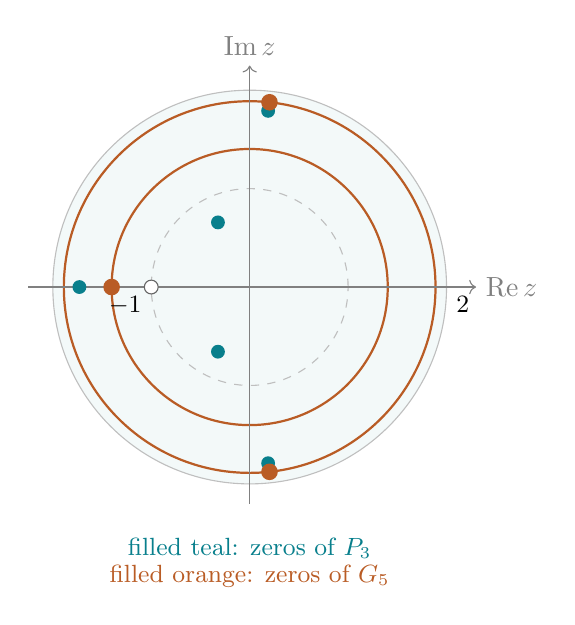
\begin{tikzpicture}[scale=1.25]
 \fill[accent!5] (0,0) circle (2);
 \draw[black!25] (0,0) circle (2);
 \draw[black!25,dashed] (0,0) circle (1);
 \draw[primefive,line width=.8pt] (0,0) circle (1.402627941186);
 \draw[primefive,line width=.8pt] (0,0) circle (1.888051164617);
 \draw[->,black!50] (-2.25,0)--(2.3,0) node[right] {$\operatorname{Re}z$};
 \draw[->,black!50] (0,-2.2)--(0,2.25) node[above] {$\operatorname{Im}z$};
 \foreach \x/\y in {-1.7300508145/0,-.3223561468/-.6568176469,-.3223561468/.6568176469,.1873815540/-1.7900150338,.1873815540/1.7900150338}
  {\fill[accent] (\x,\y) circle (2pt);}
 \foreach \x/\y in {-1.4026279412/0,.2013139706/-1.8772879069,.2013139706/1.8772879069}
  {\fill[primefive] (\x,\y) circle (2.4pt);}
 \draw[black!60,fill=white] (-1,0) circle (2pt);
 \node[below left,font=\small] at (-1,0) {$-1$};
 \node[below right,font=\small] at (2,0) {$2$};
 \node[below,font=\small,text=accent] at (0,-2.45) {filled teal: zeros of $P_3$};
 \node[below,font=\small,text=primefive] at (0,-2.73) {filled orange: zeros of $G_5$};
\end{tikzpicture}
\caption{The two circles determined by $G_5$. No zero belonging to
any other terminating prime start lies on either circle, by
Theorem~\ref{C:thm:prime-radial-separation}. The additional zero $-1$
of $P_5$ is a unit zero and is excluded. The plotted coordinates are
numerical illustrations; the separation is proved exactly.}
\label{C:fig:p5-circles}
\end{figure}

For $p=5$,
\[
 P_5(z)=(z+1)G_5(z),\qquad G_5(z)=z^3+z^2+3z+5.
\]
The cubic is irreducible by the rational-root test. Its unique real
root is $a\approx-1.402627941186$, and its nonreal roots form a
conjugate pair of common modulus $\sqrt{-5/a}$.
The two radii supplied by its nonunit factor are therefore
\[
 -a\approx1.402627941186,\qquad
 \sqrt{-5/a}\approx1.888051164617.
\]
Theorem~\ref{C:thm:prime-radial-separation} says that neither circle
contains a zero from any other terminating prime start. The additional
zero $-1$ belongs to a unit factor and is outside the theorem's scope.
Composite starts are not excluded from either circle by this theorem.
In particular, a finite check excluding the exact factor $G_5$ from
other $P_N$ does not exclude a different minimal polynomial whose roots
have the same modulus.

Having one nonunit Galois orbit is not a primality criterion. The
composite start $9$ has orbit
\[
 9,14,7,11,17,26,13,20,10,5,8,4,2,1.
\]
Its degree-$13$ polynomial is irreducible over $\mathbb Q$. Here is a
short exact certificate: its reduction modulo $2$ is
\[
 f(z)=z^{13}+z^9+z^6+z^4+z^3+z^2+1,
\]
and repeated squaring gives $z^{8192}\equiv z\pmod f$, while
$f(0)=f(1)=1$ (see the integer-only certificate accompanying Theorem~\ref{C:thm:globally-smallest-zero}). Over $\mathbb F_2$, every irreducible factor of
$z^{2^{13}}-z$ has degree dividing $13$. Since $13$ is prime and
$f$ has no linear factor, this proves that $f$ is irreducible.
Thus $P_9$ has one nonunit Galois orbit of zeros, with algebraic norm
of absolute value $9$, despite its composite starting value.
Its nonreal zeros also satisfy the irrational-angle property described
above.

These results describe exact arithmetic restrictions on locations in
the annulus. They provide no efficient algorithm for testing an unknown
starting value for primality, and no theorem that a fixed visible curve
contains zeros from all prime starts and none from composite starts.
The proofs are applications of standard algebraic-number methods;
historical novelty is not asserted.
% Self-contained proof fragment. No historical priority claim is made.
\section{Exact collisions with a prime root are quantitatively sparse}

For real $X>1$, define
\[
 A_p(X)=\#\{N\in\mathbb Z:1<N\le X,\ \tau(N)<\infty,
                         \ G_p\mid P_N\}.
\]
Equivalently, choose any root $\alpha$ of $G_p$ and count the terminating
starts whose polynomial vanishes at that exact algebraic number.
The count is independent of which conjugate root is chosen, because
$P_N(\alpha)=0$ is equivalent to $G_p\mid P_N$.

\begin{theorem}[Sparse exact collisions with a prime root]
For every odd terminating prime $p$ and every real $X>1$,
\[
 \boxed{\quad A_p(X)\le 3X^{\beta_p},\qquad
          \beta_p=\frac{\log2}{\log(2p)}<1.\quad}
\]
In particular, the set of starts sharing a root of $G_p$ has natural
density zero.  Every such start other than $p$ is composite.
\end{theorem}

\begin{proof}
We first obtain a prime-adic conjugate of the chosen root.  Normalize
the $p$-adic valuation by $v_p(p)=1$.  The polynomial $P_p$ satisfies
\[
 P_p(0)=p,\qquad P_p'(0)=\frac{3p+1}{2}\not\equiv0\pmod p.
\]
Thus $0$ is a simple root modulo $p$.  Hensel's lemma gives
$\rho\in p\mathbb Z_p$ with $P_p(\rho)=0$.
In the equation
\[
 0=p+\frac{3p+1}{2}\rho+
               \sum_{j=2}^{\tau(p)}T^j(p)\rho^j,
\]
valuation $v_p(\rho)>1$ would leave the constant term as the unique
term of smallest valuation.  Hence $v_p(\rho)=1$.
Write $P_p=G_pH_p$, where $H_p(0)=\pm1$.  Since
$H_p(\rho)\equiv H_p(0)\not\equiv0\pmod p$, the root $\rho$ belongs
to $G_p$.  Consequently every start counted by $A_p(X)$ satisfies
$P_N(\rho)=0$.

Fix an integer $r\ge1$.  For a start with $\tau(N)\ge r-1$, terms of
degree at least $r$ vanish modulo $p^r$ at $\rho$, so
\[
 0=P_N(\rho)\equiv\sum_{j=0}^{r-1}T^j(N)\rho^j\pmod {p^r}.
\]
Fixing $N$ modulo $2^{r-1}$ fixes its first $r-1$ parity decisions.
Indeed, along common initial decisions, a difference initially divisible
by $2^{r-1}$ is at each step multiplied by either $1/2$ or $3/2$;
it remains even until the last required decision.
Thus on each of these $2^{r-1}$ residue classes there are fixed integers
$s_j,b_j$ such that
\[
 T^j(N)=\frac{3^{s_j}N+b_j}{2^j}
             \qquad(0\le j\le r-1),
\]
with $s_0=b_0=0$.  Because $p$ is odd, all these rational coefficients
are $p$-adic integers.  Substituting them into the truncated evaluation
gives a congruence
\[
 U_vN+V_v\equiv0\pmod {p^r},\qquad
 U_v=\sum_{j=0}^{r-1}\frac{3^{s_j}}{2^j}\rho^j
                        \equiv1\pmod p.
\]
Here $v$ labels the chosen residue class modulo $2^{r-1}$.
The coefficient $U_v$ is a $p$-adic unit.  Therefore this equation
specifies exactly one residue class for $N$ modulo $p^r$.
By the Chinese remainder theorem, together with the chosen class modulo
$2^{r-1}$ it specifies one class modulo $2^{r-1}p^r$.
The number of counted starts with $\tau(N)\ge r-1$ is consequently at
most
\[
 2^{r-1}\left(\frac{X}{2^{r-1}p^r}+1\right)
       =\frac{X}{p^r}+2^{r-1}.
\]

The shorter orbits contribute at most $2^{r-1}$ further starts.
To see this, use $n\le2T(n)$ at every step to obtain
$N\le2^{\tau(N)}$.  If $\tau(N)<r-1$, then $N<2^{r-1}$;
for $r=1$ there are no such orbits.  We have proved, for every $r\ge1$,
\[
 A_p(X)\le\frac{X}{p^r}+2^r.
\]
Take
\[
 r=\left\lceil\frac{\log X}{\log(2p)}\right\rceil.
\]
Then $r\ge1$, $p^r\ge X^{1-\beta_p}$ and
$2^r\le2X^{\beta_p}$.  Substitution gives the claimed bound.
Since $\beta_p<1$, dividing it by $X$ proves density zero.
Finally, divisibility $G_p\mid P_N$ implies $p\mid N$ by constant
terms; hence any positive such $N\ne p$ is composite.
\end{proof}

\paragraph{Example: the prime $5$.}
Here
\[
 P_5(z)=(z+1)(z^3+z^2+3z+5),\qquad
 \beta_5=\frac{\log2}{\log10}=0.3010299956\ldots.
\]
For any exact root $\alpha$ of $z^3+z^2+3z+5$,
\[
 \#\{N\le X:\tau(N)<\infty,\ P_N(\alpha)=0\}
       \le3X^{0.3010299956\ldots}.
\]
For instance, at $X=10^6$ the exact exponent gives the upper bound
$3\cdot2^6=192$, including the known start $N=5$.
This is an upper bound, not an assertion that any additional start exists.
The exponent in the theorem is the exact logarithmic ratio, not its
displayed decimal approximation.

\paragraph{Meaning and limitations.}
The result controls exact equality of algebraic zeros, not numerical
closeness.  It is compatible with composite-start zeros being dense in
every open part of the accumulation annulus.  It does not prove that
$A_p(X)=1$ for all $X\ge p$, and it does not prove that there is even
one composite collision.  It also does not assume that all Collatz
orbits terminate: only the starts whose finite polynomials exist are
counted.  No historical priority claim is made for this deduction.

This sparsity mechanism is not an exclusive property of prime inputs.
The proof only needs a fixed algebraic root with a conjugate
$\rho\in\mathbb Q_q$ of positive valuation $v_q(\rho)=e$ at an odd
prime $q$.  In that situation the same argument uses $q^{er}$ in place
of $p^r$ and gives an exponent $\log2/\log(2q^e)$.
Suitable nonunit factors from composite starts can therefore satisfy
analogous bounds.  The theorem supplies a quantitative restriction on
possible imitators of a prime's exact root; it is not a prime-only
geometric locus or a new primality test.

\section{Shared zeros and a finite uniqueness window for prime starts}
\label{C:sec:shared-prime-roots}

Let $T(n)=n/2$ for even $n$ and $T(n)=(3n+1)/2$ for odd $n$, and let
$P_N(z)=\sum_{j=0}^{\tau(N)}T^j(N)z^j$ for a starting value whose orbit
reaches $1$. For a prime $p$, write $G_p$ for the unique monic irreducible
factor of $P_p$ whose constant term has absolute value $p$.
All other irreducible factors have constant term $1$ or $-1$.

\subsection{A prime norm does not identify a prime start}

The exact factorization
\[
 P_{10}(z)=(z+2)(z^4+4z^2+5)
\]
shows that a composite starting value can have an irreducible factor with
prime constant term. Indeed, translation by $1$ changes the quartic to
\[
 z^4+4z^3+10z^2+12z+10,
\]
which is Eisenstein at $2$. Thus the quartic is irreducible, and each of its
zeros has algebraic norm $5$, although the starting value $10$ is composite.
Those zeros satisfy $z^2=-2\pm i$, so their squared moduli are $\sqrt5$.
Prime algebraic norm, irrational squared modulus, and location strictly
inside the outer circle therefore do not, together, certify prime input.

Even an exact zero can be shared between a prime and infinitely many
composite starts. For $p=2$, $G_2(z)=z+2$, and
\[
 G_2\mid P_{2^{2r+1}}\qquad(r\geq0).
\]
This follows by substituting $-2$ in the geometric polynomial for an orbit
consisting entirely of powers of $2$. Thus the same nonunit zero $-2$
belongs to the prime start $2$ and the composite starts $8,32,128,\ldots$.
The unit zero $-1$ is also shared: it belongs to $P_5$ and to
$P_{21},P_{85},\ldots$. These facts do not decide whether a zero of $G_p$
for an odd prime can be shared with a composite start.

\subsection{A necessary divisibility pattern}

\begin{theorem}[Restriction on a shared prime factor]
\label{C:thm:shared-prime-valuations}
Let $p$ be an odd prime with a terminating orbit. Suppose $N$ terminates
and $G_p\mid P_N$. Put $k=v_2(N)$. Then
\begin{equation}
\label{C:eq:shared-prime-shape}
 N=2^k p^{k+1}u,\qquad
 u\text{ odd},\qquad u\equiv(-1)^k\pmod p.
\end{equation}
In particular, $v_p(N)=v_2(N)+1$. For odd $N$, the stronger-looking
integer congruence is
\[
 N\equiv p\pmod{2p^2}.
\]
\end{theorem}

\begin{proof}
The divisibility of constant terms first gives $p\mid N$.
The polynomial $P_p$ has constant term $p$ and linear coefficient
$(3p+1)/2$, a unit modulo $p$. Its simple zero $0$ modulo $p$ lifts to
a zero $\rho\in\mathbb Q_p$ satisfying
\[
 v_p(\rho)=1,\qquad \rho/p\equiv-2\pmod p.
\]
Every root of a monic integral polynomial has nonnegative $p$-adic
valuation. A monic factor with constant term $1$ or $-1$ can therefore
have no root of positive valuation. Consequently $\rho$ is a root of
$G_p$ and hence of $P_N$.

Write $N=2^k m$ with $m$ odd, and put $e=v_p(N)\geq1$.
Because $p\mid m$, we have $m>1$, so the coefficient following the initial
halving segment is present. The coefficients $a_j=T^j(N)$ satisfy
\[
 a_j=N/2^j\quad(0\leq j\leq k),\qquad
 a_{k+1}=(3m+1)/2.
\]
The terms $a_j\rho^j$ for $0\leq j\leq k$ have valuations $e+j$;
the term of index $k+1$ has valuation $k+1$; and every later term has
valuation at least $k+2$. Unless $e=k+1$, a unique term has smallest
valuation, making cancellation impossible. Hence $e=k+1$.

Set $N=2^k p^{k+1}u$. Divide $P_N(\rho)=0$ by $p^{k+1}$ and reduce
modulo $p$. Only the constant term and the term of index $k+1$ remain:
\[
 2^k u+\frac12(-2)^{k+1}\equiv0\pmod p.
\]
This is exactly $u\equiv(-1)^k\pmod p$. Since $k=v_2(N)$, $u$ is odd.
When $k=0$, $N/p$ is odd and congruent to $1$ modulo the odd number $p$;
therefore $N/p\equiv1\pmod{2p}$, proving the last assertion.
\end{proof}

\begin{corollary}[A finite uniqueness window]
\label{C:cor:prime-zero-window}
Let $p$ be an odd terminating prime and let $\alpha$ be a zero of $G_p$.
If $P_N(\alpha)=0$ for a terminating $N\ne p$, then
\[
 N\geq p(2p+1).
\]
More precisely, an odd such $N$ is $p+2p^2h$ for an integer $h\geq1$,
whereas an even such $N$ satisfies
\[
 N\geq2p^2(2p-1).
\]
Thus, among all terminating starts $1\leq N<p(2p+1)$, the algebraic zero
$\alpha$ identifies the starting value $p$ uniquely.
\end{corollary}

\begin{proof}
The minimal polynomial of $\alpha$ is $G_p$, so $P_N(\alpha)=0$ implies
$G_p\mid P_N$. For odd $N$, Theorem~\ref{C:thm:shared-prime-valuations}
gives $N=p+2p^2h$. Positivity implies $h\geq0$, and $N\ne p$ excludes
$h=0$.
For even $N$, consider $k=v_2(N)\geq1$. If $k=1$, the positive odd number
$u$ is $-1$ modulo $p$, and its smallest possible value is $2p-1$.
Thus $N\geq2p^2(2p-1)$. If $k\geq2$, then
$N\geq2^k p^{k+1}\geq4p^3>2p^2(2p-1)$.
Finally $2p^2(2p-1)>p(2p+1)$ for every odd prime.
\end{proof}

\begin{remark}
The congruence is necessary, not sufficient. For example $p=3$, $N=21$
satisfies it, but direct polynomial subtraction gives
\[
 P_{21}(z)=zP_3(z)+11z^2+29z+21.
\]
In fact the two polynomials are coprime: modulo $5$, the quadratic
remainder becomes $z^2-z+1$, and reducing $P_3$ modulo that polynomial
gives the nonzero constant $2$. Thus no root of $G_3$ is a root of
$P_{21}$.
The finite uniqueness result concerns an exact algebraic zero with its
minimal polynomial known. It is not a criterion based on a plotted point
or an approximate distance to a line, and it does not establish uniqueness
over unbounded starting values.
\end{remark}

\subsection{An exact line selecting one known prime in a finite range}

\begin{theorem}[A line through one algebraic zero]
\label{C:thm:transcendental-selector-line}
Let $p$ be an odd terminating prime, let $\alpha$ be a zero of $G_p$,
and let $t$ be any transcendental real number. Define the real line
\[
 L_{\alpha,t}=\{x+iy:\ y-\operatorname{Im}\alpha
                  =t(x-\operatorname{Re}\alpha)\}.
\]
The only algebraic complex number on this line is $\alpha$.
Consequently, for every terminating starting value
$1\leq N<p(2p+1)$,
\[
 P_N\text{ has a zero on }L_{\alpha,t}
 \quad\Longleftrightarrow\quad N=p.
\]
\end{theorem}

\begin{proof}
The real and imaginary parts of an algebraic complex number are algebraic,
since its complex conjugate and $i$ are algebraic. If an algebraic number
$\beta\ne\alpha$ lay on the line and had the same real part as $\alpha$,
the line equation would force the same imaginary part, a contradiction.
Otherwise that equation would give
\[
 t=\frac{\operatorname{Im}\beta-\operatorname{Im}\alpha}
         {\operatorname{Re}\beta-\operatorname{Re}\alpha},
\]
which is algebraic, again a contradiction. All zeros of $P_N$ are algebraic,
so a zero on the line must equal $\alpha$.
Corollary~\ref{C:cor:prime-zero-window} now gives $N=p$ in the stated range;
conversely $P_p(\alpha)=0$ and $\alpha$ is on the line.
\end{proof}

\paragraph{Worked example.}
Let $\alpha$ be the unique real zero of
\[
 G_5(z)=z^3+z^2+3z+5.
\]
The polynomial is irreducible by the rational-root test, and its derivative
$3z^2+2z+3$ is positive for real $z$, proving uniqueness of the real zero.
Numerically $\alpha\approx-1.402627941186$, and its exact definition is the
specified cubic root. The concrete line
\[
 \boxed{\ y=\pi(x-\alpha)\ }
\]
has a zero of $P_N$ on it, among all starts $1\leq N\leq54$ whose orbits
terminate, exactly when $N=5$. Its unique algebraic point is
$\alpha+i0$, an original zero of the Collatz polynomial $P_5$, with
$2/3<|\alpha|<2$. The bounded exact computation below extends this verified
selection property to $1\leq N\leq1000000$ for this particular example.
The displayed decimal approximation is not the definition of the intercept:
replacing $\alpha$ by a rounded rational number changes the algebraic point
selected by the line.

\begin{remark}[Scope of the construction]
This line is deliberately constructed through a zero of a known prime
start. It is a selector for that known start within the proved or checked
range, not an efficient primality algorithm for unknown integers and not
an observed universal arrangement of prime zeros. An unbounded claim would
require proving that no composite starting value shares the exact zero
$\alpha$, which is not established here for odd $p$.
The same construction works with any transcendental real slope.
Such a line has only one algebraic point, so it cannot contain infinitely
many distinct Collatz-zero locations.
\end{remark}

\subsection{An exact finite exclusion check}

For
\[
 p\in\{3,5,7,11,13,17,19,23,29\}
\]
and every $1\leq N\leq100000$, exact modular polynomial arithmetic found
\[
 G_p\mid P_N\quad\Longleftrightarrow\quad N=p.
\]
The degrees of $G_p$, in that order, are $5,3,11,10,7,9,14,11,13$.
For these starts, $G_p=P_p$ except that
$G_5=z^3+z^2+3z+5$.
This is a bounded computation, not a proof of the corresponding statement
for all positive integers.

Here is the complete verification procedure without a companion program.
Let $M=1000000007$. For each displayed $p$, compute $P_p$ from its finite
orbit and factor it over $\mathbb Q$ to obtain $G_p$.
Maintain remainders $R_N=P_N\bmod(G_p,M)$, with $R_1=1$.
For each $N=2,\ldots,100000$, follow its integer orbit until reaching a
previously processed value; then process that path backwards using
\[
 R_x=x+zR_{T(x)}\pmod{G_p,M}.
\]
This recurrence uses integer arithmetic only. Equivalently, if
$G_p=z^d+g_{d-1}z^{d-1}+\cdots+g_0$ and
$R_{T(x)}=\sum_{j=0}^{d-1}r_jz^j$, the new coefficient vector is
\[
 (x-r_{d-1}g_0,\ r_0-r_{d-1}g_1,\ldots,
 r_{d-2}-r_{d-1}g_{d-1})\pmod M.
\]
The only zero remainder with $p\mid N\leq100000$ was $N=p$ in every
case; starts not divisible by $p$ are already excluded by constant terms.
A nonzero modular remainder rigorously excludes divisibility over
$\mathbb Z$, regardless of whether the reduction of $G_p$ modulo $M$
is irreducible. This check does not require probabilistic primality tests
or floating-point approximations to zeros.

For $p=5$ alone, a separate exact integer computation extends the exclusion
through $N=1000000$. It tested all $180000$ multiples of $5$ in
$100001\leq N\leq1000000$, with no zero remainders. To reproduce it,
read each finite orbit's coefficients backwards and use Horner reduction
in $\mathbb Z[z]/(z^3+z^2+3z+5)$. If the current remainder is
$a+bz+cz^2$ and the next coefficient is $v$, the next remainder vector is
\[
 (a,b,c)\longmapsto(v-5c,\ a-3c,\ b-c).
\]
Initialize with $(0,0,0)$; after the final coefficient, divisibility holds
exactly when all three entries vanish. This extension used exact integers,
without modular filtering or numerical root comparison. The larger range
is asserted here only for $G_5$, not for the other prime starts listed above.


% Self-contained section for integration into the consolidated manuscript.
% Requires amsmath, amssymb, amsthm and the usual theorem environments.
% Additional bibliography keys:
% BakerII: A. Baker, Linear forms in the logarithms of algebraic numbers (II),
% Mathematika 14 (1967), 102--107, doi:10.1112/S0025579300008068.
% BakerIII: A. Baker, Linear forms in the logarithms of algebraic numbers (III),
% Mathematika 14 (1967), 220--228, doi:10.1112/S0025579300003843.
% No historical-priority claim is intended.

\section{Joint independence of radii, arguments, and logarithmic forms}
\label{C:sec:joint-arithmetic}

The local separation lemma (Lemma~\ref{C:lem:odd-local-zero}) and the
factor-constant partition (Proposition~\ref{C:prop:odd-factor-constants})
hold for odd composite starts as well as primes. The following extension
isolates every nonunit root, not just one selected root per prime.
The same argument applies to monic integer polynomials with coprime
constant and linear coefficients and pairwise coprime constant terms.

\begin{theorem}[All nonunit zeros are independent modulo units]
\label{C:thm:joint-root-independence}
Let $N_1,\ldots,N_t>1$ be pairwise coprime odd terminating starts.
List all the distinct nonunit zeros of their polynomials as
$\alpha_1,\ldots,\alpha_m$, including both members of every nonreal
conjugate pair.
If $\varepsilon$ is an algebraic unit and $n_1,\ldots,n_m\in\mathbb Z$
satisfy
\[
 \prod_{j=1}^m\alpha_j^{n_j}=\varepsilon,
\]
then $n_1=\cdots=n_m=0$ and $\varepsilon=1$.
In particular, these $m$ complex algebraic numbers are
multiplicatively independent.
\end{theorem}

\begin{proof}
Fix $i$, and let $f_i\in\mathbb Z[z]$ be the monic minimal polynomial
of $\alpha_i$.  Since $\alpha_i$ is a nonunit, choose a prime
$\ell\mid f_i(0)$.  The factor $f_i$ divides one of the $P_{N_a}$,
and $f_i(0)$ divides $N_a$.
The $\ell$-adic roots of $f_i$ have nonnegative valuations with
positive sum.  One therefore has positive valuation, and
Lemma~\ref{C:lem:odd-local-zero} identifies it with the unique root
$\rho$ of $P_{N_a}$ having positive valuation $e=v_\ell(N_a)$.
An embedding of $\mathbb Q(\alpha_i)$ sending $\alpha_i$ to $\rho$
extends to an embedding $\sigma$ of a number field containing all
the $\alpha_j$ and $\varepsilon$ into
$\overline{\mathbb Q}_\ell$.

Any other zero from $P_{N_a}$ has an image different from $\rho$,
by injectivity of $\sigma$, and hence has valuation zero.
For $b\ne a$, coprimality gives $\ell\nmid N_b$.
The roots of $P_{N_b}$ have nonnegative valuations whose sum is
$v_\ell(N_b)=0$, so all those valuations are zero as well.
Every image of an algebraic unit has valuation zero, since both
the unit and its inverse are integral.
Taking the valuation of the proposed identity after applying
$\sigma$ consequently gives
\[
 n_i e=0.
\]
As $e>0$, this proves $n_i=0$.  Applying the argument to every index
proves the theorem.
It also shows that a nonunit zero cannot belong to two of the
polynomials in this pairwise-coprime collection.
\end{proof}

\begin{corollary}[Independent radii modulo unit radii]
\label{C:cor:joint-radius-independence}
Choose one representative from each conjugation class of
nonunit zeros in Theorem~\ref{C:thm:joint-root-independence}, and call
their moduli $r_1,\ldots,r_k$.
For algebraic units $\varepsilon_1,\ldots,\varepsilon_s$,
\[
 \prod_{j=1}^k r_j^{u_j}
 \prod_{h=1}^s|\varepsilon_h|^{v_h}=1,
 \qquad u_j,v_h\in\mathbb Z,
\]
implies $u_1=\cdots=u_k=0$.
Thus all selected radii are different from $1$ and from one another.
\end{corollary}

\begin{proof}
Square the identity and use $|\alpha|^2=\alpha\overline\alpha$.
A nonreal conjugate pair then has exponent $u_j$ on each of its
two members; a real root has exponent $2u_j$.
The remaining factor is an algebraic unit.
Theorem~\ref{C:thm:joint-root-independence} makes every such exponent
zero.
\end{proof}

\subsection{Baker's theorem gives joint linear independence}

We use the classical, inhomogeneous form of Baker's theorem:
if complex numbers $\lambda_1,\ldots,\lambda_s$ are linearly
independent over $\mathbb Q$ and every $e^{\lambda_j}$ is algebraic,
then $1,\lambda_1,\ldots,\lambda_s$ are linearly independent over
$\overline{\mathbb Q}$.
The independence and nonzero-linear-form conclusions are due to
Baker; they are external theorems, not proved or claimed as new
here \cite{R092,R093}.

\begin{theorem}[Joint radius--argument independence]
\label{C:thm:joint-log-angle}
For the starts in Theorem~\ref{C:thm:joint-root-independence}, select
one representative of each nonunit conjugation class, choosing the
upper-half-plane root for every nonreal class.
Let $r_1,\ldots,r_k$ be all the selected moduli, and let
$\theta_1,\ldots,\theta_h\in(0,\pi)$ be the principal arguments of
the nonreal representatives.
Then
\[
 \boxed{\quad
 1,\ \pi,\ \log r_1,\ldots,\log r_k,\
 \theta_1,\ldots,\theta_h
 \quad\text{are linearly independent over }\overline{\mathbb Q}.
 \quad}
\]
All radius logarithms are real logarithms.
Arguments of real roots are omitted: all real roots are negative,
so their principal arguments equal $\pi$.
\end{theorem}

\begin{proof}
All coefficients of $P_N$ are positive, so it has no nonnegative
real root.  List its nonunit real roots as $\eta_a<0$, and its
upper-half-plane nonunit roots as $\xi_b$, with their conjugates.
For the combined collection of starts use the following fixed
logarithms:
\[
 L_0=i\pi,\qquad
 L_{\eta_a}=\log|\eta_a|+i\pi,\qquad
 L_{\xi_b}=\log|\xi_b|+i\theta_b,\qquad
 L_{\overline{\xi_b}}=\log|\xi_b|-i\theta_b.
\]
Their exponentials are respectively $-1,\eta_a,\xi_b,\overline{\xi_b}$,
all algebraic.
Suppose there is a rational linear relation between these logarithms.
After multiplying by a common denominator and exponentiating, it
becomes
\[
 (-1)^{n_0}\prod_a\eta_a^{n_a}
       \prod_b\xi_b^{u_b}\overline{\xi_b}^{v_b}=1
\]
with integer exponents.
The right-hand unit and Theorem~\ref{C:thm:joint-root-independence}
force all exponents on nonunit roots to vanish.
The original additive relation then reduces to $n_0i\pi=0$,
so $n_0=0$ too.
These logarithms are therefore linearly independent over $\mathbb Q$.
Baker's theorem makes the same logarithms, together with $1$,
linearly independent over $\overline{\mathbb Q}$.

Finally perform the following invertible change of coordinates,
whose coefficients are algebraic:
\[
 \pi=-iL_0,\qquad
 \log|\eta_a|=L_{\eta_a}-L_0,
\]
\[
 \log|\xi_b|
   =\frac{L_{\xi_b}+L_{\overline{\xi_b}}}{2},
 \qquad
 \theta_b
   =\frac{L_{\xi_b}-L_{\overline{\xi_b}}}{2i}.
\]
Its inverse is exactly the displayed definition of the $L$'s.
Linear independence over $\overline{\mathbb Q}$ is preserved,
which proves the claim.
\end{proof}

\begin{corollary}[Exact classification of ratios of linear forms]
\label{C:cor:joint-form-ratios}
Let
\[
 \mathbf v=(1,\pi,\log r_1,\ldots,\log r_k,
                    \theta_1,\ldots,\theta_h).
\]
For algebraic coefficient vectors $\mathbf a,\mathbf b$ of the
same length, with $\mathbf b\ne0$, the denominator
$\mathbf b\cdot\mathbf v$ is nonzero.  Moreover,
\[
 \frac{\mathbf a\cdot\mathbf v}{\mathbf b\cdot\mathbf v}
 \in\overline{\mathbb Q}
 \quad\Longleftrightarrow\quad
 \mathbf a=c\mathbf b
 \ \text{for some }c\in\overline{\mathbb Q}.
\]
In the proportional case the ratio equals $c$.
In every other case it is transcendental.
\end{corollary}

\begin{proof}
The denominator assertion is
Theorem~\ref{C:thm:joint-log-angle}.
If the ratio equals an algebraic number $c$, then
$(\mathbf a-c\mathbf b)\cdot\mathbf v=0$.
The same theorem implies $\mathbf a=c\mathbf b$.
The converse follows by direct substitution.
\end{proof}

\begin{corollary}[Consequences for individual angles and radii]
\label{C:cor:joint-individual-ratios}
Each $\log r_i$ and each $\theta_j$ is transcendental.
Each of the ratios
\[
 \frac{\theta_j}{\pi},\qquad
 \frac{\log r_i}{\pi},\qquad
 \frac{\theta_j}{\log r_i}
\]
is transcendental.
For distinct selected conjugation classes, the ratios of their
radius logarithms are transcendental; the same is true for the
arguments of any two distinct nonreal selected classes.
In particular, no nonreal nonunit zero has argument a rational
multiple of $\pi$.
\end{corollary}

\begin{proof}
Compare distinct coordinate vectors, or a nonconstant coordinate
vector with the coordinate vector of $1$, in
Corollary~\ref{C:cor:joint-form-ratios}.
\end{proof}

\paragraph{An explicit check against an apparent norm relation.}
For the start $5$,
\[
 P_5(z)=5+8z+4z^2+2z^3+z^4
       =(z+1)(z^3+z^2+3z+5).
\]
The cubic has no rational root, hence is irreducible.
Its derivative $3z^2+2z+3$ is positive on the real line.
It has one real root $-r$ and a nonreal pair
$R e^{\pm i\theta}$, where $r,R>0$ and $0<\theta<\pi$.
The theorem says that
\[
 1,\ \pi,\ \log r,\ \log R,\ \theta
\]
are linearly independent over $\overline{\mathbb Q}$.
Vieta's identity gives
\[
 rR^2=5,\qquad \log r+2\log R=\log5.
\]
There is no contradiction: $\log5$ is an additional number, not
an algebraic coefficient or one of the listed coordinates.
The identity becomes a dependence only after $\log5$ is adjoined.
For example, it also yields the exact classification
\[
 \frac{a\log r+b\log R}{\log5}
 \in\overline{\mathbb Q}
 \quad\Longleftrightarrow\quad b=2a
 \qquad(a,b\in\overline{\mathbb Q}),
\]
with value $a$ in the algebraic case.

\paragraph{Limits of the conclusion.}
Linear independence over $\overline{\mathbb Q}$ is not algebraic
independence: no conclusion about arbitrary polynomial relations
between these logarithms and angles is asserted.
Nor may the theorem automatically adjoin logarithms of primes
dividing the starting integers; Vieta's identity above explains why.
The theorem concerns a finite collection of exact algebraic zeros.
It supplies neither a primality criterion nor a theorem about an
uncontrolled limit of such logarithmic expressions.

\subsection{When can a nonunit radius have a rational power?}

\begin{lemma}[A root bound and the linear coefficient of a factor]
\label{C:lem:joint-small-degree}
Every zero of a terminating $P_N$ has modulus at most $2$.
If $N$ is odd and a monic integer factor
$f(z)=c+bz+\cdots$ divides $P_N$, then $\gcd(c,b)=1$.
Consequently an odd-start polynomial has no nonunit rational zero.
\end{lemma}

\begin{proof}
Write $a_j=T^j(N)$ and $d=\tau(N)$.
Since $a_{j+1}\ge a_j/2$, the coefficients $b_j=2^ja_j$ of
$Q(w)=P_N(2w)$ are positive and nondecreasing.
The identity
\[
 (1-w)Q(w)=b_0+\sum_{j=1}^d(b_j-b_{j-1})w^j-b_dw^{d+1}
\]
precludes a zero $w$ with $|w|>1$:
the modulus of the last term would exceed the sum of the moduli
of all the others, which is at most $b_d|w|^d$.
This proves the root bound.

Write $P_N=fg$ with $g\in\mathbb Z[z]$.
A prime dividing $c$ and $b$ would divide both $P_N(0)$ and
$P_N'(0)=b\,g(0)+c\,g'(0)$, which is impossible for odd $N$.
Finally a rational zero of a monic integer polynomial is an integer.
Positivity of the coefficients and the root bound leave only $-1$
and $-2$.  The latter cannot occur when $N$ is odd, by the rational
root theorem, and $-1$ is a unit.
\end{proof}

\begin{proposition}[Four precise quadratic exceptions]
\label{C:prop:joint-rational-power-exceptions}
Let $N>1$ be odd and terminating, and let $\alpha$ be a nonunit
zero of $P_N$, with $r=|\alpha|$.
The following are equivalent:
\begin{enumerate}
\item $r^b\in\mathbb Q$ for some integer $b\ge1$;
\item the monic minimal polynomial of $\alpha$ is one of
\[
 z^2+z+3,\qquad z^2-z+3,\qquad
 z^2+2z+3,\qquad z^2-2z+3.
\]
\end{enumerate}
In every such case $r=\sqrt3$ and $v_3(N)=1$.
Condition~(1) is equivalent to saying that $r$ is a rational power
of a positive rational number: clearing the denominator of the
exponent gives one direction, and $r=(r^b)^{1/b}$ gives the other.
The proposition is a conditional classification: it does not assert
that any of these four factors occurs in an odd-start Collatz
polynomial.
\end{proposition}

\begin{proof}
Assume $r^b\in\mathbb Q$ and set
$u=\alpha\overline\alpha=r^2$.
Then $u^b\in\mathbb Q$.
Let $f$ be the minimal polynomial of $\alpha$,
$d=\deg f$, and choose a prime $\ell\mid f(0)$.
Let $L$ be a splitting field of $P_N$ inside $\mathbb C$ and
$D=[L:\mathbb Q]$.
As in the proof of Theorem~\ref{C:thm:joint-root-independence}, there
is an embedding into $\overline{\mathbb Q}_\ell$ taking $\alpha$
to the unique positive-valuation root $\rho$ of $P_N$.
For that embedding, $u$ has positive valuation, since both
factors are integral and one has positive valuation.
Because $u^b$ is rational, every embedding
$\sigma:L\longrightarrow\overline{\mathbb Q}_\ell$ must give
$\sigma(u)$ the same positive valuation.
Thus for every such $\sigma$,
\[
 \sigma(\alpha)=\rho
 \quad\text{or}\quad
 \sigma(\overline\alpha)=\rho.
\]

There are $D$ embeddings in total.
Exactly $D/d$ send $\alpha$ to $\rho$, and exactly $D/d$ send
$\overline\alpha$ to $\rho$.
If $\alpha$ is nonreal these events are disjoint, so $D=2D/d$
and $d=2$.
If $\alpha$ is real they are the same event, so $D=D/d$ and
$d=1$; this is impossible for a nonunit zero by
Lemma~\ref{C:lem:joint-small-degree}.
Hence $\alpha$ is nonreal and quadratic.

Its minimal polynomial is $z^2+az+c$, where
$c=\alpha\overline\alpha=r^2$ is a positive integer.
Since $c\mid N$, it is odd; since the root is a nonunit and
$r\le2$, one has $1<c\le4$, hence $c=3$.
The discriminant is negative, so $a^2<12$.
Moreover $\gcd(a,3)=1$ by Lemma~\ref{C:lem:joint-small-degree}.
The only possibilities are $a=\pm1,\pm2$.
Conversely, every zero of any of the displayed quadratics has
modulus $\sqrt3$, proving the equivalence.
The constant term $3$ of the factor contains the entire power of
$3$ dividing $N$, by Proposition~\ref{C:prop:odd-factor-constants};
therefore $v_3(N)=1$.
\end{proof}

\begin{corollary}[Rational-base logarithmic probes]
\label{C:cor:joint-rational-base}
Under the preceding assumptions, suppose $\alpha$ does not belong
to one of the four exceptional quadratic factors.
For every rational $q>0$ with $q\ne1$,
\[
 \frac{\log|\alpha|}{\log q}
 \quad\text{is transcendental}.
\]
If an exceptional factor does occur, its radius is $\sqrt3$:
the same ratio is rational exactly when $q=3^a$ for a nonzero
integer $a$, and its value is then $1/(2a)$.
For all other positive rational $q\ne1$ the ratio is transcendental.
\end{corollary}

\begin{proof}
A rational value of the ratio implies that some positive integral
power of $|\alpha|$ is rational, excluded in the first case by
Proposition~\ref{C:prop:joint-rational-power-exceptions}.
An algebraic irrational value would contradict the
Gelfond--Schneider theorem, since $q$ and $|\alpha|$ are algebraic.

In the exceptional case the ratio is
$\log3/(2\log q)$.
Unique prime factorization of positive rational numbers shows that
it is rational exactly when $q$ is a nontrivial integer power of
$3$.  Gelfond--Schneider again excludes an algebraic irrational
value in every remaining case.
\end{proof}

\begin{corollary}[No quadratic exception for an odd prime start]
\label{C:cor:joint-prime-no-exceptions}
For any terminating odd prime $p$ and any nonunit zero $\alpha$
of $P_p$, no positive integral power of $|\alpha|$ is rational.
Consequently every rational-base ratio in
Corollary~\ref{C:cor:joint-rational-base} is transcendental.
\end{corollary}

\begin{proof}
An exceptional factor has constant term $3$, so it could divide
$P_p$ only if $p=3$.
The orbit $3,5,8,4,2,1$ gives
\[
 P_3(z)=z^5+2z^4+4z^3+8z^2+5z+3.
\]
The remainders on division by $z^2+az+3$, for
$a=-2,-1,1,2$ respectively, are
\[
 6z-39,\qquad -4z-6,\qquad -12,\qquad -10z-15.
\]
None is zero, excluding all four factors.
\end{proof}

\paragraph{The remaining quadratic question.}
No proof here excludes the four displayed quadratic factors from
every odd composite start, and no occurrence is asserted.
Eliminating them globally would strengthen the rational-base
corollary, but would not strengthen the already proved joint
independence of the selected radii and arguments.
The latter holds even if a quadratic exception exists.
The results are applications of elementary local algebra together
with the classical theorems of Baker and Gelfond--Schneider;
no claim of historical priority or of a newly resolved named
transcendence conjecture is made.


\section{Explicit transcendental quantities and what they cannot classify}
\label{C:sec:explicit-transcendental}

\subsection{An elementary logarithm test detects prime powers}
\begin{proposition}
For a fixed prime $p$ and an integer $n\ge2$,
\[
 \frac{\log n}{\log p}\in\mathbb Q
 \quad\Longleftrightarrow\quad n=p^k\quad(k\ge1).
\]
In every other case the ratio is transcendental. The same dichotomy holds
for its reciprocal.
\end{proposition}
\begin{proof}
A rational ratio $a/b$, with positive integers $a,b$, implies
$n^b=p^a$, so unique factorization makes $n$ a power of $p$.
Conversely a power gives the integer ratio $k$. If the ratio were
algebraic irrational, Gelfond--Schneider applied to $p^{\log n/\log p}=n$
would contradict the algebraicity of $n$. Taking reciprocals preserves
both rationality and transcendence for nonzero numbers.
\end{proof}
Thus a prime input $n\ne p$ and a composite input not a power of $p$
give the same transcendence answer. For example $\log7/\log5$ and
$\log21/\log5$ are both transcendental. Replacing $n$ by $n^k$ changes
the ratio by an integer factor and does not change its arithmetic type.

\subsection{A prime and a composite with the same independence pattern}
The polynomials for $N=9$ and $N=29$ both have degree $13$, are
irreducible over $\mathbb Q$, and have exactly one real root. Their
coefficient lists, in ascending powers, are
\[
\begin{split}
 P_9 &: (9,14,7,11,17,26,13,20,10,5,8,4,2,1),\\
 P_{29} &: (29,44,22,11,17,26,13,20,10,5,8,4,2,1).
\end{split}
\]
These finite statements admit exact checking. Reduction modulo $2$
certifies irreducibility for $P_9$, as detailed later; reduction modulo
$19$ does so for $P_{29}$. In the latter case the degree-$13$ polynomial
$f$ satisfies $x^{19^{13}}\equiv x\pmod f$ and
$\gcd(f,x^{19}-x)=1$ in $\mathbb F_{19}[x]$. The standard finite-field
factor criterion proves irreducibility because $13$ is prime.
Sturm's theorem gives one real root for each. A complete symbolic
check, using only exact polynomial operations, is:
\begin{lstlisting}[language=Python]
import sympy as S
x = S.symbols('x')
tails = [11,17,26,13,20,10,5,8,4,2,1]
for n, head, ell in [(9,[9,14,7],2),(29,[29,44,22],19)]:
    a = head + tails
    f = S.Poly(sum(v*x**j for j,v in enumerate(a)), x)
    g = S.Poly(f, x, modulus=ell)
    h = S.Poly(x, x, modulus=ell)
    for j in range(13):
        h = (h**ell).rem(g)
        if j == 0:
            assert S.gcd(g,h-S.Poly(x,x,modulus=ell)).degree()==0
    assert h == S.Poly(x,x,modulus=ell)
    assert f.count_roots(-S.oo,S.oo) == 1
\end{lstlisting}
Consequently each polynomial has seven distinct nonunit radii, one
for the real root and six for the nonreal pairs. The joint independence
theorem applies to both. All ratios of logarithms of different radii
are transcendental in both examples. Adding all nonunit radii from
$P_5$ gives nine independent radii in either case, since $5$ is coprime
to both $9$ and $29$. This is an exact counterexample to distinguishing
prime from composite by this independence pattern or its rank alone.
The numeric values themselves differ; equality of arithmetic type is
not equality of the numbers.

\subsection{A transcendental angle, pitch, and fractal dimension}
Write
\[
 G_5(z)=z^3+z^2+3z+5,
 \qquad Q(r)=r^3-r^2+3r-5.
\]
The derivative $Q'(r)=3r^2-2r+3$ is positive. Since $Q(1)<0<Q(3/2)$,
there is a unique root $r\in(1,3/2)$. The real zero of $G_5$ is $-r$.
Let $\alpha$ be its upper-half-plane zero and $R=|\alpha|$. Then
\[
 R^2=\frac5r,\qquad
 r\approx1.402627941186,
 \quad\alpha\approx0.201313970593+1.877287906916i.
\]
The normalized angle is
\[
 \frac{\arg\alpha}{\pi}\approx0.465995480153,
\]
and is transcendental by the joint logarithm theorem. This is stronger
than merely saying that the angle is not a rational multiple of $\pi$.
It does not say that $\arg\alpha$ alone is algebraically independent
of every familiar constant.

There is also a very general elementary observation. For any nonreal
algebraic $\beta$, put $s=|\beta|\ne1$ and choose an argument $\theta$.
Then
\[
 \frac{\theta}{\log s}\quad\hbox{is transcendental}.
\]
Indeed, if this nonzero real number $t$ were algebraic, the algebraic
irrational exponent $1+it$ would give
$s^{1+it}=\beta$, contradicting Gelfond--Schneider. In the $G_5$ example
the value is approximately $2.303483768698$. This pitch result requires
neither a prime input nor a Collatz polynomial.

\begin{proposition}[An explicit Weierstrass graph dimension]
Let $r$ be the root of $Q$ above and define
\[
 W_r(x)=\sum_{j=0}^{\infty}r^{-j}\cos(2\pi2^j x).
\]
Its graph on $[0,1]$ has transcendental Hausdorff dimension
\[
 D=2-\frac{\log r}{\log2}
   \approx1.51186762724349.
\]
\end{proposition}
\begin{proof}
The series converges uniformly because $r>1$. Shen's theorem for the
classical cosine Weierstrass function \cite{R094} applies with $b=2$
and $\lambda=1/r\in(1/2,1)$ and gives the displayed dimension.
The cubic $Q$ is irreducible by the rational-root test, and
$\operatorname{Norm}_{\mathbb Q(r)/\mathbb Q}(r)=5$.
If $\log r/\log2=a/b$ with integers $b>0$, then $r^b=2^a$;
taking norms gives $5^b=2^{3a}$, which is impossible. Gelfond--Schneider
excludes an algebraic irrational ratio. Subtracting it from $2$
therefore gives a transcendental number.
\end{proof}
The dimension formula is an established external theorem, not a
consequence of a scale-counting heuristic. The explicit application
constructs a provably transcendental dimension; it does not settle a
previously named open dimension problem.

\subsection{A self-similar set from the same cubic}
There is a second geometric realization with only rational contractions.
Let $\rho=R^2=5/r$. Substituting in $Q(r)=0$ gives
\[
 \rho^3-3\rho^2+5\rho-25=0,
\]
and the useful quartic identity is
\[
 \rho^4=\rho^3+\rho^2+15\rho+50.
\]
The quartic factors as $(x+2)(x^3-3x^2+5x-25)$.
Use the following prefix-free base-$4$ words, interpreted as the usual
subinterval maps of $[0,1]$: one word of length one, $0$; one of length
two, $10$; fifteen of length three,
\[
 \{11a,12a,13a:a=0,1,2,3\}\cup\{200,201,202\};
\]
and fifty of length four,
\[
 \{21ab,22ab,23ab:a,b=0,1,2,3\}\cup\{2030,2031\}.
\]
Their open interval images are disjoint, so the open set condition
holds. The classical self-similar dimension theorem \cite{R095}
gives the unique $d$ with
\[
 4^{-d}+4^{-2d}+15\,4^{-3d}+50\,4^{-4d}=1.
\]
Thus $4^d=\rho$ and
\[
 d=\frac{\log R}{\log2}\approx0.9168978610654274.
\]
The cubic for $\rho$ is irreducible modulo $3$ and has norm $25$.
If $\log\rho/\log4$ were rational, taking norms of a power relation
would equate a nonzero power of $25$ with a power of $4$. As before,
Gelfond--Schneider proves transcendence. This is an explicit constructed
example using a classical dimension theorem.

\subsection{Euler's constant is not the Gamma function}
The Euler--Mascheroni constant $\gamma$ and the function $\Gamma(z)$
are different objects. To use a theorem about logarithms of algebraic
numbers to prove transcendence of an independently given constant $c$,
one must first prove an \emph{exact} suitable identity, for example
$c=\log a/\log b$ for specified positive multiplicatively independent
algebraic $a,b$. A decimal match is not such an identity.

In particular, proposed identities $\log r_p=\gamma^2$ and
$\log r_q=\gamma$ would give a ratio equal to $\gamma$, but no such
identities have been established. The second alone, if true with
$r_q\ne1$ algebraic, would already prove $\gamma$ transcendental by
Hermite--Lindemann. If instead the proposal is $r_p=\gamma^2$ and
$r_q=\gamma$, the logarithmic ratio is $2$, contrary to the independent
prime-radii theorem. These are two different substitutions.

Finally, a sequence of transcendental quantities can converge to a
rational number, for example $\pi/n\to0$. Neither a boundary limit
equal to $\gamma$ nor increasingly accurate numerical approximation
proves the irrationality or transcendence of $\gamma$.


\section{Boundary distances, Euler's constant, and the zeta function}
\label{C:sec:boundary-gamma}

For the shortcut Collatz map, pure halving gives
\[
 A_m(z):=P_{2^{m-1}}(z)=\sum_{j=0}^{m-1}2^{m-1-j}z^j
 =\frac{z^m-2^m}{z-2},\qquad m\ge2.
\]
Its $m-1$ zeros are $\alpha_k=2e^{2\pi ik/m}$, $1\le k<m$.
Thus their reciprocal distances from the boundary point $2$ give
\[
 S_m:=\sum_{k=1}^{m-1}\frac1{|2-\alpha_k|}
 =\frac14\sum_{k=1}^{m-1}\csc\frac{\pi k}{m},\qquad
 E_m:=\frac{2\pi}{m}S_m-\log\frac{2m}{\pi}.
\]

\begin{proposition}[A classical cosecant asymptotic in zero coordinates]
We have $E_m\to\gamma$, where $\gamma$ is the Euler--Mascheroni constant~\cite{R070}.
More precisely,
\[
 E_m=\gamma-\frac{\pi^2}{72m^2}
       +\frac{7\pi^4}{43200m^4}+O(m^{-6}).
\]
For every $m\ge2$, the following rigorous bounds hold:
\begin{equation}\label{C:eq:boundary-gamma-bound}
 -\frac{\pi^2}{72m^2}<E_m-\gamma
 <-\frac{\pi^2}{72m^2}+\frac{7\pi^4}{43200m^4}.
\end{equation}
\end{proposition}
\begin{proof}
A self-contained proof of the limit removes the endpoint singularities:
\[
 f(x)=\csc(\pi x)-\frac1{\pi x}-\frac1{\pi(1-x)},\qquad
 \int_0^1f(x)\,dx=\frac2\pi\log\frac2\pi.
\]
The function extends smoothly to $[0,1]$. Writing $H_j$ for the
$j$th harmonic number gives the exact identity
\[
 E_m=H_{m-1}-\log m
 +\frac\pi{2m}\sum_{k=1}^{m-1}f(k/m)-\log\frac2\pi.
\]
The definition of $\gamma$ and the Riemann-sum limit prove convergence.
For the asymptotic expansion, Euler--Maclaurin summation uses
\[
 f(0)=f(1)=-1/\pi,\quad
 f'(1)-f'(0)=-\pi/3+2/\pi,
\]
\[
 f'''(1)-f'''(0)=-7\pi^3/30+12/\pi.
\]
Combining this with the harmonic-number expansion gives the displayed
coefficients. The all-$m$ inequality \eqref{C:eq:boundary-gamma-bound}
is exactly the cosecant bound of Blagouchine--Moreau~\cite{R069}, Theorem~7, equation~(74),
after multiplication by $\pi/(2m)$.
\end{proof}

\paragraph{Attribution and interpretation.}
The complete cosecant asymptotic is classical~\cite{R068,R069}, appearing in Watson's
1916 work; this is a geometric application, not a new asymptotic
formula. See G.~N.~Watson, ``The sum of a series of cosecants,''
\emph{Philosophical Magazine} 31 (1916), 111--118,
doi:10.1080/14786440208635481; and I.~V.~Blagouchine and E.~Moreau,
``On a finite sum of cosecants appearing in various problems,''
arXiv:2312.16657, Theorems~4b and~7.
The constant comes from the harmonic growth of inverse chord lengths.
The same mechanism works for regular polygons on any circle, and the
starts $2^{m-1}$ are composite for $m\ge3$.

\begin{proposition}[A finite inverse-distance zeta function]
Define, using real logarithms of the positive bases,
\[
 Z_m(s)=\frac12\sum_{k=1}^{m-1}
 \left(\frac{4\pi}{m|2-\alpha_k|}\right)^s.
\]
Then $Z_m(s)\to\zeta(s)$ locally uniformly on $\operatorname{Re}s>1$.
At the endpoint $s=1$, its logarithmic finite part is
\[
 Z_m(1)-\log(2m/\pi)=E_m\longrightarrow\gamma.
\]
\end{proposition}
\begin{proof}
Pair the terms $k$ and $m-k$. For $1\le k<m/2$ their combined
contribution is
\[
 \left(\frac{\pi}{m\sin(\pi k/m)}\right)^s\longrightarrow k^{-s}.
\]
For a compact set with $1<\sigma_0\le\operatorname{Re}s\le\sigma_1$,
the inequality $\sin(\pi k/m)\ge2k/m$ bounds these terms uniformly by
$(\pi/2)^{\sigma_1}k^{-\sigma_0}$. Dominated convergence for the
series is therefore uniform on that compact set. When $m$ is even,
the unpaired middle term $\frac12(\pi/m)^s$ tends uniformly to zero.
\end{proof}

This convergence is confined to $\operatorname{Re}s>1$. It gives no
conclusion about zeta zeros in the critical strip, the Riemann hypothesis,
or arithmetic properties of $\gamma$.

\paragraph{An exact extension beyond pure halving.}
For even $m\ge4$, set $q_m=(2^m-1)/3$ and $N_m=2^{m-1}q_m$.
The orbit has the two blocks
$q_m(2^{m-1},\ldots,1)$ and $(2^{m-1},\ldots,1)$, hence
\[
 P_{N_m}(z)=(z^m+q_m)A_m(z).
\]
Its $m-1$ boundary zeros yield exactly the same $S_m$ and $Z_m$;
the other $m$ zeros have modulus $q_m^{1/m}<2$.
These are all composite starts. For this boundary-only statistic,
$m$ is the boundary-zero count plus one, not the full degree $2m-1$.
\section{An Euler--Mascheroni limit from odd terminating starts}
\label{C:sec:gamma-odd}

This construction uses a specific infinite family of terminating odd starts.
Every member beyond $N_4=5$ is composite, so the limit below is not a
prime-detection phenomenon.

\begin{theorem}[Odd-start reciprocal-distance limit]
\label{C:thm:gamma-odd}
For even integers $m\ge4$, let
\[
 N_m=\frac{2^m-1}{3},\qquad
 P_{N_m}(z)=N_m+\sum_{j=1}^{m}2^{m-j}z^j.
\]
The displayed polynomial is the shortcut Collatz polynomial of $N_m$.
If $\alpha$ ranges over its zeros, counted with multiplicity, then
\[
 \frac{2\pi}{m}\sum_{P_{N_m}(\alpha)=0}\frac1{|2-\alpha|}
 =\log\frac{2m}{\pi}+\gamma
   +O\!\left(\frac{\log m}{m}\right)
 \qquad(m\longrightarrow\infty,\ m\ \text{even}),
\]
where $\gamma$ is the Euler--Mascheroni constant~\cite{R070}.
\end{theorem}

\begin{proof}
For even $m\ge4$, $N_m$ is odd and exceeds $1$, and
$T(N_m)=2^{m-1}$. Hence its remaining orbit consists of successive
halvings down to $1$, proving the stated polynomial formula.
Write $\epsilon_m=2^{-m}$,
\[
 b_m=\frac{1-\epsilon_m}{3},\qquad
 a_m=1-b_m=\frac{2+\epsilon_m}{3},\qquad
 D_m(w)=2^{-m}P_{N_m}(2w)=b_m+\sum_{j=1}^{m}w^j.
\]
Then
\begin{equation}\label{C:eq:gamma-odd-trinomial}
 (w-1)D_m(w)=w^{m+1}-a_mw-b_m.
\end{equation}
The right side has roots $1$ and $-1/2$; the latter uses that $m$ is even.

We first locate every other root with an error that remains uniform near
the singular point $w=1$. On $|w|>3/4$ define the principal logarithm
\[
 L_m(w)=\operatorname{Log}(a_m+b_m/w).
\]
It is holomorphic there, since the argument of the logarithm has positive
real part. Uniformly for $|w|\ge3/4$, its modulus lies between $2/9$ and
$10/9$, and the absolute value of its argument is at most
$\arcsin(2/3)$. Consequently $|L_m(w)|<2$.

Put $\zeta_j=e^{2\pi i j/m}$, $0\le j<m$. For $m\ge8$, the map
\[
 \Phi_{m,j}(u)=L_m\bigl(\zeta_j e^{u/m}\bigr)
\]
maps the closed disk $|u|\le2$ to itself, because
$|\zeta_j e^{u/m}|\ge e^{-1/4}>3/4$. Its derivative satisfies
\[
 |\Phi_{m,j}'(u)|
 =\left|\frac{-b_m}{m(a_m\zeta_j e^{u/m}+b_m)}\right|
 \le\frac2m\le\frac14.
\]
Thus it has a unique fixed point $u_j$ in that disk. The numbers
\[
 w_j=\zeta_j e^{u_j/m}
\]
satisfy $w_j^m=a_m+b_m/w_j$, hence are roots of
\eqref{C:eq:gamma-odd-trinomial}. Because $|\operatorname{Im}u_j|<\pi/2$,
they occupy disjoint angular sectors centered at the $m$th roots of unity
and are distinct. Also $u_0=0$ and $w_0=1$. The additional root $-1/2$
is outside their annulus. These $m+1$ distinct roots exhaust the
trinomial, so the roots of $D_m$ are exactly $-1/2,w_1,\ldots,w_{m-1}$.

The equality $L_m(1)=0$ gives a relative, rather than merely absolute,
root-location estimate. Along the unit circle,
\[
 \left|\frac{d}{dt}L_m(e^{it})\right|
 =\frac{b_m}{|a_me^{it}+b_m|}
 \le\frac{b_m}{a_m-b_m}\le1.
\]
Integrating along the shorter arc from $1$ to $\zeta_j$ gives
$|L_m(\zeta_j)|\le(\pi/2)|1-\zeta_j|$. The contraction estimate then
implies
\[
 |u_j|\le\frac{|L_m(\zeta_j)|}{1-2/m}
 \le\frac{2\pi}{3}|1-\zeta_j|,
 \qquad
 |w_j-\zeta_j|
 \le\frac{e^{1/4}}m|u_j|
 \le\frac3m|1-\zeta_j|.
\]
For $j\ne0$, the triangle inequality therefore yields
\begin{equation}\label{C:eq:gamma-odd-weight-error}
 \left|\frac1{|1-w_j|}-\frac1{|1-\zeta_j|}\right|
 \le\frac5m\frac1{|1-\zeta_j|}
 \qquad(m\ge8).
\end{equation}

For completeness, the corresponding roots-of-unity sum has the asymptotic
\begin{equation}\label{C:eq:gamma-cosecant-asymptotic}
 \frac\pi m\sum_{j=1}^{m-1}\frac1{|1-\zeta_j|}
 =\frac\pi{2m}\sum_{j=1}^{m-1}\csc\frac{\pi j}{m}
 =\log\frac{2m}{\pi}+\gamma+O(1/m).
\end{equation}
To see this without a singular Riemann-sum argument, subtract the two
endpoint poles and put
\[
 h(x)=\csc(\pi x)-\frac1{\pi x}-\frac1{\pi(1-x)}.
\]
The function $h$ extends to a continuously differentiable function on
$[0,1]$, with $h(0)=h(1)=-1/\pi$, and direct integration gives
\[
 \int_0^1h(x)\,dx=\frac2\pi\log\frac2\pi.
\]
Therefore the left side of \eqref{C:eq:gamma-cosecant-asymptotic} is
\[
 H_{m-1}+\frac\pi{2m}\sum_{j=1}^{m-1}h(j/m)
 =\log m+\gamma+\log\frac2\pi+O(1/m).
\]
In particular the unnormalized reciprocal-distance sum is $O(m\log m)$.
Summing \eqref{C:eq:gamma-odd-weight-error} and multiplying by $\pi/m$
changes \eqref{C:eq:gamma-cosecant-asymptotic} by
$O((\log m)/m)$. The extra root $-1/2$ contributes only $2\pi/(3m)$.
Finally $\alpha=2w$ converts $\pi/(m|1-w|)$ to
$2\pi/(m|2-\alpha|)$, completing the proof.
\end{proof}

\begin{corollary}[An explicit error bound]
Define
\[
 C_m=\frac{2\pi}{m}\sum_{P_{N_m}(\alpha)=0}\frac1{|2-\alpha|}
          -\log\frac{2m}{\pi}.
\]
For every even $m\ge8$,
\[
 \boxed{\quad |C_m-\gamma|\le\frac{5\log m+21}{m}.\quad}
\]
\end{corollary}
\begin{proof}
We make the elementary Riemann-sum error above explicit. The function
$h$ used there satisfies $|h'(x)|<8$ on $[0,1]$. Indeed, for
$0<x\le1/2$ put $t=\pi x$. The inequalities
\[
 0\le t-\sin t\le t^3/6,\qquad
 0\le1-\cos t\le t^2/2,\qquad \sin t\ge2t/\pi
\]
give
\[
 |\sin^2t-t^2\cos t|\le\frac56t^4,
 \qquad
 |h'(x)|
 \le\frac{5\pi^3}{24}+\frac4\pi<8.
\]
Symmetry $h(1-x)=h(x)$ covers the other half of the interval.
The right-endpoint Riemann sum therefore has error at most $4/m$;
removing its last endpoint, where $h(1)=-1/\pi$, gives
\[
 \left|\frac1m\sum_{j=1}^{m-1}h(j/m)-\int_0^1h(x)\,dx\right|
 \le\frac{4+1/\pi}{m}.
\]
Together with
$|H_{m-1}-\log m-\gamma|\le1/m$, this yields
\[
 \left|B_m-\log\frac{2m}{\pi}-\gamma\right|
 \le\frac{2\pi+3/2}{m}<\frac8m,
 \qquad
 B_m=\frac\pi m\sum_{j=1}^{m-1}\frac1{|1-\zeta_j|}.
\]
In particular $B_m\le\log m+2$ for $m\ge8$, using $\gamma<1$.
The relative bound \eqref{C:eq:gamma-odd-weight-error} and the contribution
$2\pi/(3m)$ of the outlier give
\[
 |C_m-\gamma|
 \le\frac{5B_m+8+2\pi/3}{m}
 \le\frac{5\log m+21}{m},
\]
as claimed.
\end{proof}

\begin{corollary}[First logarithmic correction]
With the notation of Theorem~\ref{C:thm:gamma-odd},
\[
 \frac{2\pi}{m}\sum_{P_{N_m}(\alpha)=0}\frac1{|2-\alpha|}
 -\log\frac{2m}{\pi}
 =\gamma+\frac{\log m}{3m}+O(1/m).
\]
In particular the normalized quantities eventually exceed $\gamma$.
\end{corollary}
\begin{proof}
The fixed-point estimates in the proof give, uniformly for $1\le j<m$,
\[
 w_j=\zeta_j+\frac{\zeta_jL_m(\zeta_j)}m
           +O\!\left(\frac{|1-\zeta_j|}{m^2}\right).
\]
Define
\[
 A_m(\zeta)=\frac{\zeta L_m(\zeta)}{1-\zeta},\qquad A_m(1)=b_m.
\]
The apparent singularity at $1$ is removable, since $L_m'(1)=-b_m$.
On the unit circle these functions are uniformly bounded and satisfy
$A_m(\zeta)-b_m=O(|1-\zeta|)$; this follows from uniform bounds for
the derivatives of $L_m$ near $1$, and compactness away from $1$.
Consequently
\[
 \frac1{|1-w_j|}
 =\frac1{|1-\zeta_j|}
   \left(1+\frac{\operatorname{Re}A_m(\zeta_j)}m+O(m^{-2})\right).
\]
If $B_m$ denotes the roots-of-unity sum on the left side of
\eqref{C:eq:gamma-cosecant-asymptotic}, summation and the bounded remainder
$\bigl(\operatorname{Re}A_m(\zeta)-b_m\bigr)/|1-\zeta|$ give
\[
 \frac\pi m\sum_{D_m(w)=0}\frac1{|1-w|}
 =B_m+\frac{b_m}{m}B_m+O(1/m).
\]
The root $-1/2$ is included in the $O(1/m)$ term. Substituting
$B_m=\log(2m/\pi)+\gamma+O(1/m)$ and
$b_m=1/3+O(2^{-m})$ proves the formula. Its positive logarithmic term
eventually dominates the $O(1/m)$ remainder.
\end{proof}

The uniform relative bound \eqref{C:eq:gamma-odd-weight-error} is essential:
weak convergence of root-counting measures alone would not justify this
limit, because the reciprocal-distance kernel is unbounded at $w=1$.

To verify the compositeness claim, write $m=2r\ge6$. Then
\[
 N_m=\frac{(2^r-1)(2^r+1)}3.
\]
Exactly one of the two factors is divisible by $3$. After dividing that
factor by $3$, both factors exceed $1$ because $r\ge3$. Thus the same
Euler--Mascheroni limit holds along this explicit family of odd composites.

\paragraph{Numerical illustration and reproduction.}
The following values illustrate the convergence. They are ordinary
floating-point approximations, not interval certificates or substitutes
for the proof. The reference value is
$\gamma\approx0.577215664901533$.
\begin{center}
\begin{tabular}{r r}
$m$ & Approximate $C_m$\\\hline
$128$ & $0.607570723152$\\
$2048$ & $0.579564141044$\\
$32768$ & $0.577390648950$\\
$131072$ & $0.577262936443$
\end{tabular}
\end{center}
The complete Python code below uses only its standard library and
implements the contraction proved above. Conjugate pairs are counted
together, and the exact scaled outlier $-1/2$ is included separately.
No external script or polynomial root-finding package is required.
For large $m$, floating-point underflow replaces $2^{-m}$ by zero;
the analytic proof uses its exact value throughout.
\begingroup\small
\begin{lstlisting}[language=Python]
import cmath
import math

def gamma_approx(m):
    assert m >= 8 and m % 2 == 0
    b = (1 - 2.0**(-m)) / 3
    a = 1 - b
    weights = [2/3]
    for j in range(1, m//2 + 1):
        zeta = cmath.exp(2j * math.pi * j / m)
        u = 0j
        for step in range(30):
            v = cmath.log(a + b / (zeta * cmath.exp(u/m)))
            if abs(v-u) < 2e-16:
                u = v
                break
            u = v
        w = zeta * cmath.exp(u/m)
        weight = 1 / abs(1-w)
        weights.append(weight if 2*j == m else 2*weight)
    total = math.pi/m * math.fsum(weights)
    return total - math.log(2*m/math.pi)

for m in (128, 2048, 32768, 131072):
    print(m, format(gamma_approx(m), '.12f'))
\end{lstlisting}
\endgroup



\section{Stability of the Euler limit and its complete first correction}
\label{C:sec:gamma-stability-refinement}

The appearance of Euler's constant in the preceding distance sums is an
endpoint phenomenon.  The first two statements below isolate elementary
forms of that mechanism; they are not claims of a new general theory of
Euler's constant.  The final theorem evaluates the full coefficient of
$m^{-1}$ for the specific odd Collatz family, refining the earlier
$O(m^{-1})$ remainder after the logarithmic correction.

\begin{lemma}[Endpoint subtraction]
\label{C:lem:endpoint-subtraction-general}
Suppose that
\[
 k(x)=\frac{a_0}{x}+\frac{a_1}{1-x}+g(x),\qquad 0<x<1,
\]
where $a_0,a_1$ are fixed real numbers and $g$ is Lipschitz continuous on
$[0,1]$.  Then
\[
 \frac1m\sum_{j=1}^{m-1}k(j/m)
 =(a_0+a_1)(\log m+\gamma)+\int_0^1g(x)\,dx+O(m^{-1}).
\]
\end{lemma}
\begin{proof}
The two pole sums are exactly $(a_0+a_1)H_{m-1}$.  The remaining sum
is a Riemann sum for $g$ with error $O(m^{-1})$, and
$H_{m-1}=\log m+\gamma+O(m^{-1})$.
\end{proof}

For the inverse-chord kernel $k(x)=\pi/(2\sin\pi x)$ one has
$a_0=a_1=1/2$ and $\int_0^1g=\log(2/\pi)$.  Thus the two sides
of the singular point jointly produce one copy of the harmonic sum.
The additional logarithm in $\log(2m/\pi)$ removes a geometric
constant.  A different grid or kernel need not have the same finite
part, and the mere presence of logarithmic divergence does not force
the constant to be $\gamma$.

\begin{proposition}[Relative perturbation stability]
\label{C:prop:gamma-relative-stability}
Fix $R>0$ and write $\zeta_{m,j}=e^{2\pi i j/m}$ for $1\le j<m$.
Suppose a multiset of points contains $m-1$ labelled points
$\alpha_{m,j}$ satisfying
\[
 |\alpha_{m,j}-R\zeta_{m,j}|
 \le \delta_m R|1-\zeta_{m,j}|,
 \qquad 0\le\delta_m<1,
\]
and additional points $\beta_{m,\ell}\ne R$, counted with multiplicity.
Set
\[
 B_m=\frac\pi m\sum_{j=1}^{m-1}\frac1{|1-\zeta_{m,j}|},
 \qquad
 U_m=\frac{\pi R}{m}
 \left(\sum_{j=1}^{m-1}\frac1{|R-\alpha_{m,j}|}
       +\sum_\ell\frac1{|R-\beta_{m,\ell}|}\right).
\]
Then
\[
 \left|U_m-\log\frac{2m}{\pi}-\gamma\right|
 \le \frac{\pi^2}{72m^2}
 +\frac{\delta_m}{1-\delta_m}B_m
 +\frac{\pi R}{m}\sum_\ell\frac1{|R-\beta_{m,\ell}|}.
\]
In particular, if $\delta_m\log m\to0$ and
$\sum_\ell |R-\beta_{m,\ell}|^{-1}=o(m)$, then
\[
 U_m-\log\frac{2m}{\pi}\longrightarrow\gamma.
\]
\end{proposition}
\begin{proof}
Put $d_j=R|1-\zeta_{m,j}|$.  The triangle inequality gives
$\bigl||R-\alpha_{m,j}|-d_j\bigr|\le\delta_m d_j$, so
\[
 \left|\frac1{|R-\alpha_{m,j}|}-\frac1{d_j}\right|
 \le\frac{\delta_m}{1-\delta_m}\frac1{d_j}.
\]
Sum this estimate and use the classical cosecant bound
\eqref{C:eq:boundary-gamma-bound}, which implies
$|B_m-\log(2m/\pi)-\gamma|\le\pi^2/(72m^2)$.
Finally $B_m=O(\log m)$.
\end{proof}

This proposition explains why an absolute error estimate or weak
convergence of zero-counting measures is insufficient near the
singular point.  It also shows that no Collatz-specific or prime-specific
mechanism is needed once the required relative perturbation estimate
has been established.

\begin{theorem}[The full coefficient of the first correction]
\label{C:thm:gamma-full-first-correction}
For the odd family of Theorem~\ref{C:thm:gamma-odd}, define
\[
 C_m=\frac{2\pi}{m}\sum_{P_{N_m}(\alpha)=0}\frac1{|2-\alpha|}
            -\log\frac{2m}{\pi},
 \qquad
 u=\arcsin\frac1{\sqrt3}.
\]
As $m\to\infty$ through even integers,
\[
 C_m=\gamma+\frac{\log m}{3m}+\frac{K}{m}
                  +O\!\left(\frac{\log m}{m^2}\right),
\]
where
\[
 \boxed{\displaystyle
 K=\frac{\gamma+\log(2/\pi)}3
       +u^2-\frac{2\sqrt2}{3}u+\frac13+\frac{2\pi}{3}.}
\]
Numerically, $K\approx2.26814152647080423359$.
\end{theorem}
\begin{proof}
Keep the notation $b=b_m=(1-2^{-m})/3$, $a=1-b$, and
$\zeta_j=e^{2\pi i j/m}$ from the odd-family proof.  For
$0\le b\le1/3$ put
\[
 L_b(\zeta)=\operatorname{Log}(1-b+b/\zeta),\qquad
 A_b(\zeta)=\frac{\zeta L_b(\zeta)}{1-\zeta},\qquad A_b(1)=b.
\]
The logarithm is the principal branch.  The expression is analytic in
a fixed annulus around the unit circle, and the apparent singularity of
$A_b$ at $1$ is removable.  All bounds below are uniform in
$b\in[0,1/3]$.

The contraction proof gives $|u_j|=O(|1-\zeta_j|)$ and
$u_j-L_b(\zeta_j)=O(|1-\zeta_j|/m)$.  Expanding
$w_j=\zeta_j e^{u_j/m}$ therefore yields
\[
 w_j=\zeta_j+\frac{\zeta_jL_b(\zeta_j)}m
                 +O\!\left(\frac{|1-\zeta_j|}{m^2}\right).
\]
It follows, uniformly for $1\le j<m$, that
\[
 \frac1{|1-w_j|}
 =\frac1{|1-\zeta_j|}
 \left(1+\frac{\operatorname{Re}A_b(\zeta_j)}m+O(m^{-2})\right).
\]

Define
\[
 f_b(x)=\frac{\operatorname{Re}A_b(e^{2\pi i x})-b}
                    {|1-e^{2\pi i x}|},\qquad 0<x<1.
\]
These functions extend to $f_b(0)=f_b(1)=0$ and are uniformly
Lipschitz.  To check the endpoint assertion explicitly,
$A_b(\overline\zeta)=\overline{A_b(\zeta)}$ makes
$\operatorname{Re}A_b(e^{it})$ an even smooth function near $t=0$.
Its difference from $b$ is therefore $O(t^2)$, with derivative
$O(|t|)$, whereas $|1-e^{it}|$ is comparable to $|t|$.
Compactness handles the rest of the circle.  Consequently
\[
 \frac1m\sum_{j=1}^{m-1}f_b(j/m)=\int_0^1 f_b(x)\,dx+O(m^{-1}).
\]
Writing $J(b)=\pi\int_0^1f_b(x)\,dx$, including the exact outlier
$w=-1/2$, and using $B_m=O(\log m)$ now gives
\begin{equation}\label{C:eq:gamma-full-correction-reduction}
 \frac\pi m\sum_{D_m(w)=0}\frac1{|1-w|}
 =B_m+\frac{b}{m}B_m+\frac{J(b)}m+\frac{2\pi}{3m}
       +O\!\left(\frac{\log m}{m^2}\right).
\end{equation}

It remains to evaluate $J$.  Symmetry around the real axis gives
\[
 J(b)=\int_0^\pi
 \frac{\operatorname{Re}A_b(e^{it})-b}{2\sin(t/2)}\,dt.
\]
The uniform endpoint estimates justify differentiation under the
integral sign.  Since
\[
 \frac{\partial A_b(\zeta)}{\partial b}
       =\frac1{1-b+b/\zeta},
\]
one obtains
\[
 J'(b)=\int_0^\pi
 \frac{b(1-2b)\sin(t/2)}{1-4b(1-b)\sin^2(t/2)}\,dt.
\]
The substitution $v=\cos(t/2)$ evaluates this as
\[
 J'(b)=2\sqrt{\frac b{1-b}}\arcsin\sqrt b
        \qquad(0\le b\le1/3).
\]
Using $J(0)=0$ and then the substitution $s=\arcsin\sqrt b$ gives
\[
 J(b)=(\arcsin\sqrt b)^2
       -2\sqrt{b(1-b)}\arcsin\sqrt b+b.
\]
Finally, the earlier classical expansion supplies
$B_m=\log(2m/\pi)+\gamma+O(m^{-2})$, while
$b_m=1/3+O(2^{-m})$.  Insert these expressions into
\eqref{C:eq:gamma-full-correction-reduction} to obtain the claimed $K$.
\end{proof}

\begin{corollary}[An accelerated expression without an unknown input]
\label{C:cor:gamma-accelerated-expression}
Put
\[
 J_0=u^2-\frac{2\sqrt2}{3}u+\frac13,
 \qquad
 \widehat\gamma_m=
 \frac{mC_m-\frac13\log(2m/\pi)-J_0-2\pi/3}{m+1/3}.
\]
Then
\[
 \widehat\gamma_m=\gamma
          +O\!\left(\frac{\log m}{m^2}\right).
\]
Every quantity in the definition of $\widehat\gamma_m$ is determined
by the finite Collatz polynomial and elementary constants; the
unknown target $\gamma$ is not supplied as an input.
\end{corollary}
\begin{proof}
In the preceding theorem, collect the terms containing $\gamma$ and
multiply by $m$.  Division by $m+1/3$ gives the result.
\end{proof}

The acceleration is a consequence of an asymptotic expansion, not a
transcendence criterion.  In particular, the formulas do not establish
the irrationality of $\gamma$ or identify $e^\gamma$ with an algebraic
zero.


\section{What a geometric primality criterion would need to detect}

Write $T(n)=n/2$ for even $n$, and $T(n)=(3n+1)/2$ for odd $n$.
For a start $N$ which reaches $1$, let $\tau(N)$ be the first such time and put
\[
 P_N(z)=\sum_{j=0}^{\tau(N)}T^j(N)z^j.
\]
Its leading coefficient is $1$ and its constant coefficient is $N$.
Consequently its complete root multiset determines $N$ by Vieta's formula.
Recovering $N$ this way and applying an ordinary primality test is an exact
reformulation, but it supplies neither a new primality test nor a prime-only
line in the complex plane.

\subsection{An exact polynomial certificate and the first failing degree}

The following constructive certificate applies to the reciprocal Collatz
polynomial, but the proof is a general binomial argument.  It belongs to the
same classical polynomial-congruence principle as Lemma 2.1 of
Agrawal--Kayal--Saxena, \emph{PRIMES is in P} (2004); no claim of a new
primality-testing principle or efficiency improvement is made.

\begin{theorem}[First failure of a Frobenius congruence]
Let $N\geq2$, and let $F(z)\in\mathbb Z[z]$ satisfy
$F(0)=1$ and $\gcd(F'(0),N)=1$.  Set
\[
 D_{N,F}(z)=F(z)^N-F(z^N).
\]
Then
\[
 N\text{ is prime}\quad\Longleftrightarrow\quad
 D_{N,F}(z)\equiv0\pmod N.
\]
If $N$ is composite and $q$ is its least prime divisor, then the least
degree having a nonzero coefficient in $D_{N,F}$ modulo $N$ is exactly $q$.
More precisely, if $e=v_q(N)$, then
\[
 v_q\bigl([z^q]D_{N,F}(z)\bigr)=e-1.
\]
In particular, it is enough to check that the coefficients in degrees
$1,\ldots,\lfloor\sqrt N\rfloor$ all vanish modulo $N$.
\end{theorem}

\begin{proof}
For prime $N$, the Frobenius identity in $\mathbb F_N[z]$ and the congruence
$a^N\equiv a\pmod N$ for integer coefficients $a$ give
$F(z)^N\equiv F(z^N)\pmod N$.

Suppose $N$ is composite, let $q$ be its least prime divisor, and write
$F=1+U$, where $U(0)=0$ and $a=U'(0)$ is coprime to $N$.  For $1\leq j<N$,
the term $F(z^N)$ has zero coefficient in degree $j$, and the binomial
theorem gives
\[
 [z^j]D_{N,F}
 =\sum_{k=1}^{j}\binom Nk[z^j]U(z)^k.
\]
Terms $k>j$ contribute nothing because $U(0)=0$.
When $j<q$, each $1\leq k\leq j$ is coprime to $N$; from
$k\binom Nk=N\binom{N-1}{k-1}$ we obtain $N\mid\binom Nk$.
Thus all degrees below $q$, including degree zero, vanish modulo $N$.

Write $e=v_q(N)$.  For $k<q$ the same identity implies
$v_q\binom Nk\geq e$.  However,
\[
 \binom Nq=\frac Nq\binom{N-1}{q-1},\qquad
 \binom{N-1}{q-1}\equiv(-1)^{q-1}\not\equiv0\pmod q,
\]
so $v_q\binom Nq=e-1$.  Since $[z^q]U^q=a^q$ is a $q$-adic unit,
\[
 [z^q]D_{N,F}\equiv\binom Nq a^q\pmod {q^e}
\]
has valuation exactly $e-1$.  This coefficient does not vanish modulo $N$,
proving the characterization and the first-failure claim.  Finally, every
composite $N$ has a least prime divisor $q\leq\sqrt N$, proving the
truncated coefficient criterion.
\end{proof}

\begin{corollary}[Reciprocal Collatz polynomial certificate]
For odd $N>1$ whose orbit reaches $1$, let $d=\tau(N)$ and
\[
 R_N(z)=z^dP_N(1/z)=1+2z+\cdots+Nz^d.
\]
Then $N$ is prime if and only if
\[
 R_N(z)^N\equiv R_N(z^N)\pmod N.
\]
For composite odd $N$, the first nonzero coefficient of the difference
modulo $N$ occurs precisely at its least prime divisor.
\end{corollary}

\begin{proof}
The last state before the first occurrence of $1$ is $2$: the even equation
$n/2=1$ has solution $n=2$, whereas $(3n+1)/2=1$ has no positive integer
solution.  Hence $R_N(0)=1$, $R_N'(0)=2$, and the theorem applies because
$N$ is odd.
\end{proof}

\paragraph{An exact algorithm.}
Handle $N\leq1$, $N=2$, and even $N>2$ immediately.  For odd $N$, choose
an admissible $F$ (for example $R_N$ if a terminating orbit is supplied),
and let $B=\lfloor\sqrt N\rfloor$.  Compute
\[
 H(z)=F(z)^N\pmod{(N,z^{B+1})}
\]
by repeated squaring with truncated polynomial multiplication.  If
$H(z)=1$, return PRIME.  Otherwise, the least positive degree with nonzero
coefficient is the least prime divisor of $N$, and return COMPOSITE with
that divisor.  The proof above verifies this algorithm since $B<N$ and
$F(z^N)\equiv1\pmod {z^{B+1}}$.

\paragraph{What is and is not gained.}
This supplies a coefficient-level if-and-only-if test and even an exact
factor location for composite inputs.  It is not a prime-only line in the
original complex zero annulus.  The exponent and truncation length depend
on $N$, and the $\sqrt N$ bound is exponential in the bit length of $N$.
More fundamentally, $F(z)=1+z$ already satisfies all hypotheses for every
$N\geq2$, so the Collatz orbit is unnecessary for this test.  Taking that
choice also removes any dependence on an unproved universal termination
claim.  The later, much more substantial reductions in the AKS algorithm
are not established merely by this congruence.



\section{Exact primality encodings by boundary power maps}
\label{C:sec:boundary-prime-encodings}
Here an integer power map $u\mapsto u^a$ is called a fold in the earlier
construction. It is distinct from the two axis reflections considered
in Section~\ref{C:sec:two-folds}.
\subsection{A factorial encoding using one boundary zero}
\label{C:sec:factorial-folding}

The construction in this section is an exact reformulation of classical
primality arithmetic. It uses a known boundary zero of a very simple
Collatz polynomial and the Gelfond--Schneider theorem. It is not a new
primality algorithm, and it does not classify the starting value of an
arbitrary Collatz polynomial from its unmodified zeros.

\begin{lemma}[A root-of-unity logarithm dichotomy]
\label{C:lem:fold-log-dichotomy}
Fix a prime $p\ge3$ and let $u$ be any root of unity. Put
\[
 R=p+|1-u|^2=p+2-u-u^{-1},\qquad
 L=\frac{\log R}{\log p},
\]
where the logarithms are real. If $u=1$, then $L=1$. If $u\ne1$, then
$L>1$ is transcendental.
\end{lemma}
\begin{proof}
The number $R$ is an algebraic integer. Every conjugate of $R$ is of
the form $p+2-v-v^{-1}=p+|1-v|^2$, where $v$ is a root of unity.
Thus every conjugate is positive and lies in $[p,p+4]$.

Suppose first that $L=a/b\in\mathbb Q$, with $b>0$. Then $R^b=p^a$.
Each conjugate of $R$ must therefore be the unique positive real
$b$th root of $p^a$. All conjugates are equal, so separability in
characteristic zero implies $R\in\mathbb Q$. A rational algebraic
integer is an integer. Unique factorization in $\mathbb Z$ now gives
$R=p^k$ for an integer $k\ge0$. Since
\[
 p\le R\le p+4<p^2\qquad(p\ge3),
\]
we must have $R=p$, hence $u=1$ and $L=1$.

If $u\ne1$, we have therefore excluded rational $L$. Were $L$
algebraic irrational, the Gelfond--Schneider theorem would make
$p^L=R$ transcendental, contrary to the algebraicity of $R$.
Consequently $L$ is transcendental. Finally $u\ne1$ gives $R>p$,
so $L>1$.
\end{proof}

\begin{theorem}[Prime versus composite after a factorial fold]
\label{C:thm:factorial-fold-prime}
Fix any prime reference $p\ge3$. For every integer $n\ge2$, define
\[
 A_n=((n-1)!)^2,\qquad \zeta_n=e^{2\pi i/n},
\]
\[
 R_n=p+|1-\zeta_n^{A_n}|^2,\qquad
 L_n=\frac{\log R_n}{\log p}.
\]
Then
\[
 \boxed{
 \begin{aligned}
 n\text{ prime}&\quad\Longleftrightarrow\quad
       L_n\text{ transcendental},\\
 n\text{ composite}&\quad\Longleftrightarrow\quad L_n=1.
 \end{aligned}}
\]
In the prime case,
$R_n=p+2-2\cos(2\pi/n)$.
\end{theorem}
\begin{proof}
If $n$ is prime, Wilson's congruence gives $(n-1)!\equiv-1\pmod n$,
and hence $A_n\equiv1\pmod n$. For completeness, the congruence follows
by pairing every nonzero residue modulo $n$ with its inverse; the
unpaired residues are $1,-1$ when $n$ is odd. The case $n=2$ is immediate.
Thus $\zeta_n^{A_n}=\zeta_n\ne1$, and
Lemma~\ref{C:lem:fold-log-dichotomy} gives the transcendence assertion.

If $n$ is composite, write $n=ab$ with $1<a,b<n$. Both $a$ and $b$
divide $(n-1)!$. Writing $(n-1)!=ar=bs$ shows
\[
 ((n-1)!)^2=abrs=nrs.
\]
This argument also covers $a=b$ and $n=4$. Consequently
$A_n\equiv0\pmod n$, $\zeta_n^{A_n}=1$, and $L_n=1$.
Every integer $n\ge2$ is either prime or composite, so both
equivalences follow.
\end{proof}

\paragraph{The exact Collatz connection.}
For the shortcut Collatz map, start at $N=2^{n-1}$. Its orbit is the
halving chain $2^{n-1},2^{n-2},\ldots,1$, and its polynomial is
\[
 P_{2^{n-1}}(z)=\sum_{j=0}^{n-1}2^{n-1-j}z^j
 =2^{n-1}\sum_{j=0}^{n-1}(z/2)^j.
\]
Thus $\alpha_n=2\zeta_n$ is an actual zero on the boundary $|z|=2$.
The theorem may equivalently be written using
\[
 R_n=p+\left|1-(\alpha_n/2)^{A_n}\right|^2.
\]
This identifies the primality of the index $n$, not the primality of the
Collatz starting value $2^{n-1}$. The latter is composite for every
$n\ge3$. The prime/composite information enters through the factorial
congruence; the boundary zero supplies a geometric representation of
that congruence, and the logarithm changes its output to $1$ versus a
transcendental number.

The same conclusion holds simultaneously for every nontrivial $n$th
root $\zeta_n^k$, $1\le k<n$: prime $n$ leaves all these folded roots
nontrivial, while composite $n$ sends every one to $1$. Therefore all
corresponding logarithms are transcendental in the prime case, and all
are $1$ in the composite case. The single primitive root already
suffices for the stated criterion.

\paragraph{Exact examples with $p=5$.}
\begin{center}
\begin{tabular}{c c c c}
$n$ & $A_n\bmod n$ & $R_n$ & $L_n$\\\hline
$2$ & $1$ & $9$ & transcendental\\
$3$ & $1$ & $8$ & transcendental\\
$4$ & $0$ & $5$ & $1$\\
$5$ & $1$ & $(15-\sqrt5)/2$ & transcendental\\
$6$ & $0$ & $5$ & $1$\\
$7$ & $1$ & $7-2\cos(2\pi/7)$ & transcendental\\
$9$ & $0$ & $5$ & $1$
\end{tabular}
\end{center}
The transcendent entries are proved by the lemma, not inferred from
decimal approximations. In actual computation one would calculate
$((n-1)!)^2\bmod n$ directly; numerical testing of transcendence offers
no shortcut. No claim of historical novelty is made for this
repackaging of classical results.

% Primary source for the logarithmic consequence of Gelfond--Schneider:
% A. Baker, Linear forms in the logarithms of algebraic numbers,
% Mathematika 13 (1966), 204--216, doi:10.1112/S0025579300003971.
% Cambridge extract explicitly states algebraic-base algebraic-number
% logarithms are rational or transcendental. Also Jonathan Pila,
% https://people.maths.ox.ac.uk/pila/Nex.pdf, Theorem 3.2, p.9.

\subsection{A factorial-free product using all boundary zeros}
\label{C:sec:chord-product-classifier}

The following construction gives an exact prime/composite equivalence
using products of squared chord lengths. Its arithmetic content is the
classical absence of zero divisors modulo a prime. The construction
requires no primality label as input and no factorial. No claim of a new
efficient primality algorithm or of historical novelty is made.

\begin{lemma}[The folded chord product]
\label{C:lem:folded-chord-product}
For each integer $n\ge2$, let $\zeta_n=e^{2\pi i/n}$ and define
\[
 D_n=\prod_{j=1}^{n-1}\prod_{k=1}^{n-1}
           |1-\zeta_n^{jk}|^2.
\]
Then
\[
 \boxed{D_n=
 \begin{cases}
 n^{2(n-1)},&n\text{ prime},\\
 0,&n\text{ composite}.
 \end{cases}}
\]
\end{lemma}
\begin{proof}
Suppose first that $n=q$ is prime. For each $1\le j<q$, multiplication
by $j$ permutes the nonzero residue classes modulo $q$. Moreover
\[
 \prod_{r=1}^{q-1}(x-\zeta_q^r)=1+x+\cdots+x^{q-1},
 \qquad
 \prod_{r=1}^{q-1}(1-\zeta_q^r)=q.
\]
Consequently each inner product in $D_q$ equals
\[
 \prod_{k=1}^{q-1}|1-\zeta_q^{jk}|^2
 =\left|\prod_{r=1}^{q-1}(1-\zeta_q^r)\right|^2=q^2.
\]
There are $q-1$ such products, proving $D_q=q^{2(q-1)}$.

If $n$ is composite, write $n=ab$ with $1<a,b<n$. The indices
$j=a$, $k=b$ occur in the product and give
$|1-\zeta_n^{ab}|^2=|1-1|^2=0$. Hence $D_n=0$.
\end{proof}

\begin{theorem}[An exact transcendence criterion with a fixed prime base]
\label{C:thm:chord-product-prime}
Fix any prime $p\ge2$. For $n\ge2$, define
\[
 F_p(n)=\frac{\log(p+D_n)}{\log p}.
\]
Then
\[
 \boxed{
 \begin{aligned}
 n\text{ prime}&\quad\Longleftrightarrow\quad
          F_p(n)\text{ transcendental},\\
 n\text{ composite}&\quad\Longleftrightarrow\quad F_p(n)=1.
 \end{aligned}}
\]
In the prime case $F_p(n)>1$. The reference prime $p$ is fixed
independently of the tested integer $n$.
\end{theorem}
\begin{proof}
For a composite $n$, Lemma~\ref{C:lem:folded-chord-product} gives
$D_n=0$ and hence $F_p(n)=1$.

Now let $n=q$ be prime and put $M=p+q^{2(q-1)}$. We first show that
$M$ is not an integer power of $p$. If $q\ne p$, then $p\nmid M$,
since $M\equiv q^{2(q-1)}\not\equiv0\pmod p$. If $q=p$, then
\[
 M=p\bigl(1+p^{2p-3}\bigr).
\]
Here $2p-3\ge1$, so the exponent of $p$ in $M$ is exactly $1$,
whereas $M>p$. This also excludes a power of $p$. In particular
the case $n=p=2$ is covered: $M=6$.

If $\log M/\log p=a/b\in\mathbb Q$, with $b>0$, then
$M^b=p^a$. Unique factorization forces the positive integer $M$ to
be an integer power of $p$, a contradiction. Thus $F_p(q)$ is
irrational. If it were algebraic irrational, the Gelfond--Schneider
theorem would make $p^{F_p(q)}=M$ transcendental, contradicting the
fact that $M$ is an integer. Therefore $F_p(q)$ is transcendental.
Finally $M>p$ proves $F_p(q)>1$, and the two exhaustive cases give
both stated equivalences.
\end{proof}

\paragraph{The exact connection with all Collatz boundary zeros.}
Use the shortcut Collatz map $T(N)=N/2$ for even $N$ and
$T(N)=(3N+1)/2$ for odd $N$, stopping at the first $1$. The orbit of
$2^{n-1}$ is its halving chain, so
\[
 P_{2^{n-1}}(z)=\sum_{r=0}^{n-1}2^{n-1-r}z^r
 =2^{n-1}\sum_{r=0}^{n-1}(z/2)^r.
\]
Its zeros are precisely
\[
 \alpha_j=2\zeta_n^j,\qquad 1\le j<n.
\]
Every one lies on the outer circle $|z|=2$. Therefore the chord product
can be written entirely in terms of these zeros and their integer folds:
\[
 \boxed{D_n=
 \prod_{P_{2^{n-1}}(\alpha)=0}\ 
 \prod_{k=1}^{n-1}\left|1-(\alpha/2)^k\right|^2.}
\]
The product uses every zero. If $n$ is prime, no listed fold lands at
$1$, and the product has the exact positive value $n^{2(n-1)}$.
If $n$ is composite, at least one listed fold lands at $1$, and one
zero chord makes the entire product vanish.

\paragraph{Exact examples with $p=5$.}
\begin{center}
\begin{tabular}{c r r c}
$n$ & $D_n$ & $5+D_n$ & $F_5(n)$\\\hline
$2$ & $4$ & $9$ & $\log 9/\log 5$ (transcendental)\\
$3$ & $81$ & $86$ & $\log 86/\log 5$ (transcendental)\\
$4$ & $0$ & $5$ & $1$\\
$5$ & $390625$ & $390630$ & transcendental\\
$6$ & $0$ & $5$ & $1$
\end{tabular}
\end{center}

\paragraph{Scope of the criterion.}
The tested integer is $n=\deg P_{2^{n-1}}+1$. This does not test the
primality of the Collatz starting value $2^{n-1}$, which is composite
for $n\ge3$. It also makes no primality assertion about the transformed
integer $p+D_n$: for example, $p=5$, $n=2$ gives $p+D_n=9$.

The result expresses a classical divisibility criterion through the
geometry of known Collatz boundary zeros, then uses a standard
transcendence theorem to give its output a different form. Numerical
testing of transcendence supplies no computational shortcut. Directly
evaluating a product with $(n-1)^2$ factors is not an asserted
improvement over established primality algorithms. Nothing here proves
a prime-only locus among the unmodified zeros of arbitrary $P_N$.

% Primary source for the logarithmic consequence of Gelfond--Schneider:
% A. Baker, Linear forms in the logarithms of algebraic numbers,
% Mathematika 13 (1966), 204--216, doi:10.1112/S0025579300003971.
% Cambridge extract explicitly states algebraic-base algebraic-number
% logarithms are rational or transcendental. Also Jonathan Pila,
% https://people.maths.ox.ac.uk/pila/Nex.pdf, Theorem 3.2, p.9.

\paragraph{An entirely integral version.}
Let $A_n(x)=(x^n-1)/(x-1)$. The same chord product is
\[
 D_n=\prod_{k=1}^{n-1}\operatorname{Res}(A_n(x),1-x^k)^2.
\]
Indeed, the resultant is the product of $1-\zeta_n^{jk}$ over $1\le j<n$;
it is $n$ if $\gcd(k,n)=1$ and zero otherwise. Thus exact resultants
remove numerical root coordinates, but expose the same ordinary
modular divisibility test. They do not create a faster transcendence
oracle.


% Standalone section fragment. Requires amsmath, amsthm, amssymb,
% booktabs, and hyperref in the parent document. No external program or
% data file is required: the complete executable verification is below.
\section{A known prime as a certificate for a larger integer}
\label{C:sec:seed-primality}

This appendix records the exact primality statements investigated after
the zero-geometry questions. The results belong to classical
large-factor primality theory. They do not constitute a new general
primality algorithm, a consequence of the Collatz conjecture, or a
method for deciding arbitrary integers from one previously known prime.
In particular, a single displayed congruence is not a constant-time
computation. Its evaluation may require substantial arithmetic.

\subsection{An exact one-base test on a specified family}

\begin{theorem}[A classical large-prime-factor criterion]
\label{C:thm:seed-one-base}
Let $P$ be a proven odd prime, let $k$ be a positive even integer, and
put $N=kP+1$. If
\begin{equation}
  2^k<N<(2P+1)^2,
  \label{C:eq:seed-range}
\end{equation}
then
\begin{equation}
  N\text{ is prime}
  \quad\Longleftrightarrow\quad
  2^{N-1}\equiv1\pmod N.
  \label{C:eq:seed-iff}
\end{equation}
\end{theorem}

\begin{proof}
If $N$ is prime, the congruence follows from Fermat's little theorem,
since $N$ is odd. Conversely, assume the congruence and write
$d=\operatorname{ord}_N(2)$. Then $d\mid kP$. The inequality
$1<2^k<N$ shows that $2^k\not\equiv1\pmod N$, so $d\nmid k$.
If $P\nmid d$, coprimality of $d$ and $P$ would imply $d\mid k$;
therefore $P\mid d$. Lagrange's theorem gives $d\mid\varphi(N)$,
and hence $P\mid\varphi(N)$.

Write $N=\prod_j q_j^{e_j}$. Because $N\equiv1\pmod P$, no $q_j$
equals $P$. The product formula
\[
 \varphi(N)=\prod_j q_j^{e_j-1}(q_j-1)
\]
therefore implies $P\mid q-1$ for some prime divisor $q$ of $N$.
Suppose $N$ is composite and set $h=N/q>1$. Reduction modulo $P$
gives $q\equiv h\equiv1\pmod P$. Both $q$ and $h$ are odd.
Since $P$ is odd, an odd integer greater than $1$ and congruent to
$1$ modulo $P$ is at least $2P+1$. Consequently
\[
  N=qh\ge(2P+1)^2,
\]
contrary to \eqref{C:eq:seed-range}. Thus $N$ is prime.
\end{proof}

The order argument is part of the classical $N-1$ theory of
Pocklington and Brillhart--Lehmer--Selfridge
\cite{R076,R077}; the explicit $kP+1$ specialization
also appears in \cite[Theorem~2.1]{R078}.
The hypotheses matter: without them, a base-$2$ Fermat congruence
alone is only a probable-prime condition. For example,
$341=11\cdot31$ satisfies $2^{340}\equiv1\pmod{341}$.

\begin{corollary}[Mersenne seeds]
\label{C:cor:mersenne-seed-range}
Suppose $P=2^m-1$ is prime and $m\ge3$. For every even integer
$k$ with $2\le k\le m$, the number $N_k=kP+1$ satisfies
\eqref{C:eq:seed-range}. Thus \eqref{C:eq:seed-iff} is an exact
primality test for each such $N_k$.
\end{corollary}

\begin{proof}
We have $2^k\le2^m=P+1<2P+1\le N_k$.
Also $m\le P$, so
$N_k\le P^2+1<(2P+1)^2$.
\end{proof}

This corollary neither predicts that one of the candidates is prime
nor proves that infinitely many of them are prime. It specifies a
finite family on which one congruence is conclusive. Failure of that
congruence proves compositeness; success proves primality under the
stated hypotheses.

\subsection{Exact examples and reproducible certificates}

For $P=127=2^7-1$, exact modular exponentiation gives
\[
  2^{508}\bmod509=1,\qquad
  2^{762}\bmod763=64.
\]
Since $509=4P+1$ and $763=6P+1$ satisfy the range conditions,
Theorem~\ref{C:thm:seed-one-base} proves that $509$ is prime and $763$
is composite. Indeed, $763=7\cdot109$.

For the larger seed $P=2^{127}-1$, the following two candidates also
have residue $1$ and are therefore proven primes:
\begin{center}
\small
\begin{tabular}{@{}rll@{}}
\toprule
$k$ & $N=k(2^{127}-1)+1$ & $2^{N-1}\bmod N$\\
\midrule
114 & 19396094914493492417412352623610788052879 & 1\\
124 & 21097506749098184734729225660769629110149 & 1\\
\bottomrule
\end{tabular}
\end{center}
Both integers have $41$ decimal digits. These computations certify
their primality; they do not assert that these integers were previously
unknown primes.

For completeness, the seed certificates use the classical
Lucas--Lehmer theorem \cite{R079}: for a prime exponent $m\ge3$, define
$s_0=4$ and $s_{j+1}=s_j^2-2\pmod{2^m-1}$. Then $2^m-1$ is prime
if and only if $s_{m-2}=0$. The exponents $7$ and $127$ are themselves
verified by trial division in the complete Python code below. The
code uses only exact integers and the Python standard library. It
contains all data needed for these examples and the following
small-divisor table; no separate source file or numerical package is
required.

\begingroup\small
\begin{lstlisting}[language=Python]
from math import isqrt

def small_prime(n):
    return n >= 2 and all(n % d for d in range(2, isqrt(n)+1))

def mersenne_prime(m):
    assert small_prime(m)
    p = (1 << m) - 1
    if m == 2:
        return p
    s = 4
    for _ in range(m-2):
        s = (s*s - 2) % p
    assert s == 0                 # Lucas--Lehmer certificate
    return p

def classify(p, k):
    # Precondition: p has already been PROVEN prime.
    n = k*p + 1
    assert p > 2 and k > 0 and k % 2 == 0
    assert (1 << k) < n < (2*p + 1)**2
    residue = pow(2, n-1, n)
    return n, residue, ('prime' if residue == 1 else 'composite')

p7 = mersenne_prime(7)
assert classify(p7, 4) == (509, 1, 'prime')
assert classify(p7, 6) == (763, 64, 'composite')

p127 = mersenne_prime(127)
expected = {
    114: 19396094914493492417412352623610788052879,
    124: 21097506749098184734729225660769629110149,
}
for k, value in expected.items():
    assert classify(p127, k) == (value, 1, 'prime')

m = 136279841
factors = (3, 5, 607, 3, 11, 281, 3, 7, 13, 3, 103, 5, 3)
for k, q in zip(range(2, 28, 2), factors):
    assert small_prime(q)
    assert (k*(pow(2, m, q)-1)+1) % q == 0
print('All certificates and small-divisor identities verified.')
\end{lstlisting}
\endgroup

\subsection{What can be checked cheaply at the record-sized seed}

Set $M=2^{136279841}-1$. For the candidates $N_k=kM+1$, the
following exact proper divisors already prove compositeness:
\begin{center}
\small
\begin{tabular}{@{}r*{13}{r}@{}}
\toprule
$k$ & 2&4&6&8&10&12&14&16&18&20&22&24&26\\
$q\mid N_k$ &3&5&607&3&11&281&3&7&13&3&103&5&3\\
\bottomrule
\end{tabular}
\end{center}
Each entry is checked by the small computation
\[
 k\bigl((2^{136279841}\bmod q)-1\bigr)+1\equiv0\pmod q.
\]
It is unnecessary to construct the decimal expansion of $M$ or
evaluate a modular power with modulus $N_k$. These divisibility
certificates do not even require an assumption that $M$ is prime.
In contrast, applying Corollary~\ref{C:cor:mersenne-seed-range} to a
candidate that survives such sieving requires a certified prime seed
and a potentially very expensive congruence computation. No prime
larger than $M$ is certified by this table, and failure to find a small
divisor is not a primality proof.

\subsection{Related certificates and the boundary of the method}

\begin{proposition}[Pocklington certificate]
\label{C:prop:seed-pocklington}
Let $N>1$, and let $F\mid N-1$ have a complete factorization into
proven primes, with $F>\sqrt N$. Suppose that for every prime $q\mid F$
there is an integer $a_q$ satisfying
\[
 a_q^{N-1}\equiv1\pmod N,\qquad
 \gcd\bigl(a_q^{(N-1)/q}-1,N\bigr)=1.
\]
Then $N$ is prime.
\end{proposition}

\begin{proof}
For each prime divisor $r$ of $N$, the order of $a_q$ modulo $r$
divides $N-1$ but does not divide $(N-1)/q$. Its $q$-adic valuation
is therefore $v_q(N-1)$. As the order divides $r-1$, this implies
$F\mid r-1$. Hence every prime divisor of $N$ exceeds $\sqrt N$,
which is impossible for a composite $N$.
\end{proof}

With a single known prime $P$, one may extract
$F=P^{v_P(N-1)}$ by repeated division, without factoring the
remaining cofactor. If $F^2>N$, the proposition supplies a useful
certificate. Its failure for a particular base does not by itself
prove compositeness: a greatest common divisor equal to $N$ can simply
mean that another base is needed. A proper greatest common divisor,
or a failed Fermat congruence, does prove compositeness.

There is a precise $N+1$ analogue using Lucas sequences. Let $N$ be
odd, $P$ a proven odd prime dividing $N+1$, and
\[
 U_0=0,\quad U_1=1,\quad U_{j+2}=A U_{j+1}-B U_j,
 \qquad \Delta=A^2-4B.
\]
If $\gcd(N,2B\Delta)=1$,
$U_{N+1}\equiv0\pmod N$,
$\gcd(U_{(N+1)/P},N)=1$, and $2P-1>\sqrt N$, then $N$ is prime.
Indeed, for each prime $r\mid N$, the rank of apparition of $r$ in
this Lucas sequence divides $r-(\Delta/r)$ and, by the two displayed
conditions on $U$, is divisible by $P$. Thus $r\equiv\pm1\pmod P$.
Oddness gives $r\ge2P-1>\sqrt N$. This is a certificate, not an
unconditional binary test for an arbitrary fixed choice of $A,B$;
see the classical $N+1$ theory in \cite{R077}.

An elliptic-curve certificate provides a different route
\cite{R080}. Let $E$ be an elliptic curve modulo $N$ with
discriminant coprime to $N$. Suppose a point $R$ reduces to a
nonidentity point modulo every prime divisor of $N$, and
\[
 [Q]R=O,\qquad Q\text{ is a proven prime},\qquad
 Q>(N^{1/4}+1)^2.
\]
Then $N$ is prime: if a prime $r\le\sqrt N$ divided $N$, reduction
would give a point of order $Q$ over $\mathbb F_r$, contrary to
Hasse's bound
$Q\le\#E(\mathbb F_r)\le(\sqrt r+1)^2\le(N^{1/4}+1)^2$.
The nonidentity condition must hold at every prime divisor, not merely
as a formal inequality $R\ne O$ over a composite modulus. Finding a
suitable curve, point, and certified $Q$ is a separate computational
problem. None of these certificates guarantees a short proof for an
arbitrary prescribed $N$ from one fixed seed prime.



% Self-contained contribution; insert in the main document before the bibliography.
% Requires amsmath, amssymb, amsthm, hyperref and theorem/proposition environments.
\section{External constants: established applications and unresolved extensions}
\label{C:sec:ext-targets}

The arithmetic arguments for Collatz zero moduli invite comparison with constants
that were defined independently of this investigation.  Such a comparison must
distinguish an application of an established theorem from the solution of a
previously open problem.  This section supplies several exact applications,
then records the hypotheses that fail for harder targets.  No previously open
named constant is claimed to be classified here.

\subsection{A reusable criterion for logarithms of algebraic units}

We use real logarithms of positive real numbers.  The
Gelfond--Schneider theorem implies the familiar dichotomy
\begin{equation}
 \alpha,\beta\in\overline{\mathbb Q}\cap\mathbb R_{>0},\quad
 \alpha\ne1,\quad\beta\ne1
 \quad\Longrightarrow\quad
 \frac{\log\alpha}{\log\beta}\in\mathbb Q
 \ \text{or}\ 
 \frac{\log\alpha}{\log\beta}\text{ is transcendental}.
 \label{C:eq:ext-log-dichotomy}
\end{equation}
Indeed, an algebraic irrational value $t$ would make $\beta^t=\alpha$
transcendental, a contradiction.  This is classical transcendence theory,
not a property specific to Collatz trajectories; see \cite{R067}.

An algebraic unit is an algebraic number $u$ for which both $u$ and $u^{-1}$
are algebraic integers.  Its norm in any number field containing it is $1$ or
$-1$.

\begin{proposition}[Unit logarithms]
\label{C:prop:ext-unit-log}
If $u>1$ is an algebraic unit and $b\ge2$ is an integer, then
$\log u/\log b$ is transcendental.
\end{proposition}
\begin{proof}
If the ratio were rational, write it as $m/n$ with positive integers $m,n$.
Then $u^n=b^m$.  In a number field $K$ containing $u$, taking norms gives
$(\pm1)^n=b^{m[K:\mathbb Q]}$, which is impossible.  Apply
\eqref{C:eq:ext-log-dichotomy}.
\end{proof}

Thus the same norm calculation can certify transcendence in a setting with no
distinguished prime divisor at all.  It distinguishes an algebraic unit from
an integer greater than one; it does not automatically distinguish two
different units from each other.

\subsection{Hard-square strips: a complete finite-width calculation}

In the hard-square model, occupied sites of a square lattice may not be
adjacent.  At activity $1$, its partition function counts independent sets of
the grid graph.  Transfer matrices encode compatibility between consecutive
rows; their standard definition is given in \cite[Section~2]{R081}.

Fix a width $w\ge1$ with open boundary conditions across a row.  Let
$\mathcal F_w$ be the family of independent subsets of the path with $w$
vertices.  Put
\begin{equation}
 A_{ST}=\mathbf1_{S\cap T=\varnothing}\qquad(S,T\in\mathcal F_w).
 \label{C:eq:ext-transfer}
\end{equation}
The family $\mathcal F_w$ is downward closed: every subset of an allowed row
is allowed.  This simple fact determines the determinant of $A$ exactly.

\begin{proposition}[Compatibility factorization]
\label{C:prop:ext-factorization}
Let $\mathcal F$ be a finite nonempty downward-closed family of subsets of a
finite set.  Define $A$ by \eqref{C:eq:ext-transfer}, with indices in
$\mathcal F$, and set
\[
 Z_{SU}=\mathbf1_{U\subseteq S},\qquad
 D_{UU}=(-1)^{|U|}.
\]
Then
\begin{equation}
 A=ZDZ^{\mathsf T},\qquad
 \det A=(-1)^{\sum_{U\in\mathcal F}|U|}.
 \label{C:eq:ext-zdz}
\end{equation}
Every eigenvalue of $A$ is an algebraic unit.
\end{proposition}
\begin{proof}
For $S,T\in\mathcal F$, downward closure gives
\[
 (ZDZ^{\mathsf T})_{ST}
 =\sum_{U\subseteq S\cap T}(-1)^{|U|}
 =\begin{cases}1,&S\cap T=\varnothing,\\0,&S\cap T\ne\varnothing.
 \end{cases}
\]
Order $\mathcal F$ by nondecreasing cardinality.  Then $Z$ is lower
triangular with all diagonal entries equal to $1$.  This proves the
determinant formula.  In particular, $A$ is invertible over $\mathbb Z$.
An eigenvalue $\lambda$ is an algebraic integer because $A$ is integral;
$\lambda^{-1}$ is an algebraic integer because $A^{-1}$ is integral.
\end{proof}

The factorization is the elementary subset-poset form of the classical
M\"obius factorization for meet matrices.  The proof is included to avoid
any dependence on a numerical determinant calculation.  It also applies to
independent subsets of a cycle and, more generally, of any finite graph.

Let $\lambda_w$ be the spectral radius of the open-strip matrix $A$.
Since the empty row is compatible with every row, $A^2$ is entrywise
positive.  Perron--Frobenius theory therefore gives a simple positive
dominant eigenvalue.  The principal submatrix on the empty row and any
one-site row is
\[
 \begin{pmatrix}1&1\\1&0\end{pmatrix},
\]
so $\lambda_w\ge(1+\sqrt5)/2>1$.  Proposition~\ref{C:prop:ext-factorization}
and Proposition~\ref{C:prop:ext-unit-log} prove
\begin{equation}
 \boxed{\quad\frac{\log\lambda_w}{\log b}\text{ is transcendental
 for every }w\ge1\text{ and integer }b\ge2.\quad}
 \label{C:eq:ext-strip-result}
\end{equation}
The same is true after division by $w$, which expresses strip entropy per
site in base $b$.  For example, at width $1$ it gives the transcendence of
$\log((1+\sqrt5)/2)/\log2$.

At every finite prime of every number field containing an eigenvalue,
the valuation of that eigenvalue is zero.  Thus a method requiring a
nonzero valuation at a distinguished prime cannot be transferred unchanged
to this model.  Formula~\eqref{C:eq:ext-strip-result} succeeds for a different
reason: the comparison number $b$ is not a unit.

\subsection{Why the infinite-width limit remains a different problem}

If $I(n,n)$ counts independent sets of an $n$ by $n$ square grid, the
hard-square growth constant is
\[
 \kappa_2=\lim_{n\to\infty}I(n,n)^{1/n^2}
 =1.503048\ldots.
\]
It can also be approached through increasing strip widths.  The 2026
preprint \cite{R082} explicitly treats the algebraicity of this limit
as unresolved.  Finite transfer matrices have algebraic eigenvalues, but
their dimensions and the associated number fields grow with the width.
Neither their unit property nor \eqref{C:eq:ext-strip-result} classifies the
limit.

The following exact example shows that this is a logical obstruction, not
merely a missing error estimate.

\begin{proposition}[Transcendental logarithm ratios can converge to a rational]
\label{C:prop:ext-unit-limit}
For $n\ge2$, let $u_n>2$ be the real root of
\[
 x^n-2x^{n-1}-1=0.
\]
Then $u_n$ is an algebraic unit,
$\log u_n/\log2$ is transcendental, and
\[
 \lim_{n\to\infty}\frac{\log u_n}{\log2}=1.
\]
\end{proposition}
\begin{proof}
The function $x^{n-1}(x-2)$ increases strictly from $0$ to infinity on
$(2,\infty)$, so the stated root exists and is unique.  Its monic
polynomial has constant term $-1$; the reciprocal also satisfies a monic
integral polynomial.  Hence $u_n$ is a unit.  Moreover,
\[
 0<u_n-2=u_n^{-(n-1)}<2^{-(n-1)}.
\]
This proves $u_n\to2$, while Proposition~\ref{C:prop:ext-unit-log}
proves transcendence at each finite index.
\end{proof}

Consequently, even a convergent sequence consisting entirely of units,
with explicitly transcendental normalized logarithms, supplies no such
classification of its limit without an additional uniform argument.

\subsection{Gamma values: a transcendental combination need not identify a factor}

Euler's gamma function $\Gamma$ must be distinguished from the
Euler--Mascheroni constant $\gamma$.  A classical theorem of Schneider on
abelian integrals proves the transcendence of
\begin{equation}
 B\left(\frac15,\frac15\right)
 =\frac{\Gamma(1/5)^2}{\Gamma(2/5)}.
 \label{C:eq:ext-beta-fifth}
\end{equation}
See \cite{R083,R084}.  It follows that $\Gamma(1/5)$ and
$\Gamma(2/5)$ cannot both be algebraic.  It does not identify which
individual value is transcendental.  Algebraicity of $\Gamma(1/5)$ alone
would be compatible with \eqref{C:eq:ext-beta-fifth} if $\Gamma(2/5)$ were
transcendental.  Grinspan's stronger result states that at least one of
these two gamma values is transcendental over $\mathbb Q(\pi)$
\cite{R085}; the conclusion still does not isolate a specified
one of them.

Nor does taking logarithms turn these numbers into an instance of
\eqref{C:eq:ext-log-dichotomy}.  That theorem requires its logarithm
arguments to be algebraic.  Substituting gamma values whose required
arithmetic nature has not been established assumes the missing hypothesis.
Similarly, for a positive $x\ne1$,
\[
 \frac{\log(x^2)}{\log x}=2
\]
is an identity for every such $x$, and cannot classify $x$.

\subsection{Somos's constant: the finite versus infinite logarithm issue}

Somos's quadratic recurrence constant has the convergent product and series
\begin{equation}
 \sigma=\prod_{n=1}^{\infty}n^{2^{-n}},\qquad
 \log\sigma=\sum_{n=1}^{\infty}2^{-n}\log n.
 \label{C:eq:ext-somos}
\end{equation}
Sondow and Hadjicostas \cite{R086} connect it to the
generalized Euler-constant function
\[
 \gamma_{\mathrm{gen}}(z)
 =\sum_{n\ge1}z^{n-1}
 \left(\frac1n-\log\frac{n+1}{n}\right),
 \qquad
 \gamma_{\mathrm{gen}}(1/2)=2\log(2/\sigma).
\]
This is a useful exact identity, but it transfers the same unknown
arithmetic information between two expressions.

Every finite product
$\sigma_N=\prod_{n=1}^{N}n^{2^{-n}}$ is algebraic; for $N\ge2$ it is
greater than one.  Its real logarithm is transcendental by the
Hermite--Lindemann theorem.  The limit in \eqref{C:eq:ext-somos} is an
infinite logarithmic sum, whereas Baker's linear-independence results
apply to finitely many logarithms of algebraic numbers.

One can make the failure of a naive prime-by-prime reduction explicit.
All summands are nonnegative, so rearranging the real series gives
\begin{equation}
 \log\sigma=\sum_{p\text{ prime}}c_p\log p,
 \qquad
 c_p=\sum_{j\ge1}\frac1{2^{p^j}-1}.
 \label{C:eq:ext-somos-primes}
\end{equation}
Indeed,
$\sum_{n\ge1}2^{-n}v_p(n)
=\sum_{j\ge1}\sum_{k\ge1}2^{-kp^j}$.
Formula~\eqref{C:eq:ext-somos-primes} has infinitely many nonzero
coefficients, and it does not establish that those coefficients are
algebraic.  It therefore meets neither the finiteness condition nor the
coefficient hypothesis of the usual finite logarithm theorem.  Furthermore,
real convergence alone does not justify taking a $p$-adic valuation of an
infinite product.  These observations leave the arithmetic classification
of $\sigma$ unresolved by the present methods.

\subsection{The sophomore's dream: rapid convergence is not enough}

Another independently established target is
\begin{equation}
 S=\sum_{n=1}^{\infty}\frac1{n^n}
 =\int_0^1x^{-x}\,dx.
 \label{C:eq:ext-dream}
\end{equation}
The integral identity follows by expanding
$e^{-x\log x}$ into its nonnegative power series and integrating:
$\int_0^1x^k(-\log x)^k\,dx=k!/(k+1)^{k+1}$.
Han\v{c}l and Kristensen discuss its unresolved irrationality in their
2018 work \cite{R087}; no resolution is claimed here.

Let $S_N=\sum_{n=1}^{N}n^{-n}$ and use the natural common denominator
\[
 D_N=\operatorname{lcm}(1^1,2^2,\ldots,N^N).
\]
The tail $R_N=S-S_N$ obeys the elementary bounds
\begin{equation}
 (N+1)^{-(N+1)}\le R_N
 \le\frac{N+2}{N+1}(N+1)^{-(N+1)}.
 \label{C:eq:ext-dream-tail}
\end{equation}
For the upper bound, successive terms in the tail have ratio at most
$1/(N+2)$.  On the other hand, every prime $p\in(N/2,N]$ contributes
the factor $p^p$ to $D_N$.  Writing
$\vartheta(x)=\sum_{p\le x}\log p$, the prime number theorem yields
\[
 \log D_N\ge\sum_{N/2<p\le N}p\log p
 \ge\frac N2\bigl(\vartheta(N)-\vartheta(N/2)\bigr)
 \ge cN^2
\]
for some $c>0$ and all sufficiently large $N$.  Together with
\eqref{C:eq:ext-dream-tail}, this proves
\begin{equation}
 D_NR_N\longrightarrow\infty.
 \label{C:eq:ext-denominator-obstruction}
\end{equation}

If $S=a/b$ were rational, then $bD_NR_N$ would be an integer.  The usual
elementary contradiction would require that positive integer to lie below
$1$; \eqref{C:eq:ext-denominator-obstruction} shows why this particular
denominator-and-tail argument cannot do so.  This does not rule out better
approximants or cancellation in the reduced denominator of $S_N$.  It
identifies the failure of the displayed method, not an impossibility theorem
for proving irrationality.

\subsection{Established modular examples really do admit stronger conclusions}

There are external infinite series for which a deeper theorem supplies
the missing structure.  Define
\[
 L_k=\sum_{n\ge1}\frac{n^k}{2^n-1},\qquad k=1,3,5.
\]
These three constants are algebraically independent, hence each is
transcendental.  This is an established consequence of Nesterenko's modular
theorem \cite{R088}, not a new application of a Collatz argument.
For completeness, put
\[
 \begin{split}
 E_2(q)&=1-24\sum_{n\ge1}\frac{nq^n}{1-q^n},\\
 E_4(q)&=1+240\sum_{n\ge1}\frac{n^3q^n}{1-q^n},\\
 E_6(q)&=1-504\sum_{n\ge1}\frac{n^5q^n}{1-q^n}.
 \end{split}
\]
Nesterenko proves that, for $0<|q|<1$, the field
$\mathbb Q(q,E_2(q),E_4(q),E_6(q))$ has transcendence degree at least
$3$.  At the algebraic point $q=1/2$, this forces the three series values
to be algebraically independent.  The displayed rational affine changes
of variables give the assertion for $L_1,L_3,L_5$.

Related established consequences include the transcendence of
\[
 \theta_3(1/2)=\sum_{n\in\mathbb Z}2^{-n^2}
 \qquad\text{and}\qquad
 \sum_{n\ge1}\frac1{F_n^2},
\]
where $F_1=F_2=1$ are the Fibonacci numbers; see
\cite[Theorem~46 and Corollaries~51--52]{R089}.
The reciprocal-square series must not be confused with
$\sum_{n\ge1}1/F_n$.  These examples show what an effective external
connection requires: an exact identification with functions covered by a
substantial theorem, rather than numerical resemblance or a shared use of
the word ``zero.''

\subsection{The Moser--de Bruijn decimal constant: an explicit classical proof}

Let $E$ consist of the nonnegative integers whose base-$4$ digits belong to
$\{0,1\}$:
\[
 E=\{0,1,4,5,16,17,20,21,\ldots\}.
\]
The established decimal construction
\begin{equation}
 \chi=3\sum_{n\in E}10^{-n}
 =3.300330000000000330033\ldots
 \label{C:eq:ext-moser}
\end{equation}
appears in van der Poorten's discussion of an observation of Blanchard and
Mend\`es France \cite{R090}.  Its transcendence is already accessible
to Roth's theorem.  The proof below is recorded as a transparent classical
application, not as a newly solved open problem.

\begin{proposition}
The number $\chi$ in \eqref{C:eq:ext-moser}, and its reciprocal, are
transcendental.
\end{proposition}
\begin{proof}
Put $M_k=(4^k-1)/3$ and truncate at the last position representable with
$k$ base-$4$ digits:
\[
 \chi_k=3\sum_{\substack{n\in E\\n\le M_k}}10^{-n}
 =\frac{A_k}{q_k},\qquad q_k=10^{M_k}.
\]
Since $M_k\in E$, the integer $A_k$ ends in the decimal digit $3$.
Thus $\gcd(A_k,q_k)=1$.  The next nonzero digit occurs at position $4^k$,
and therefore
\begin{equation}
 0<\chi-\frac{A_k}{q_k}
 \le3\sum_{j=4^k}^{\infty}10^{-j}
 =\frac{10}{3}10^{-4^k}
 =\frac1{3q_k^3}.
 \label{C:eq:ext-moser-roth}
\end{equation}
The decimal expansion has infinitely many nonzero digits and arbitrarily
long zero blocks.  It is neither terminating nor ultimately periodic, so
$\chi$ is irrational.  If it were algebraic, Roth's theorem
\cite{R091}, for example with exponent $2+1/2$, would allow only
finitely many reduced rational approximations satisfying
\eqref{C:eq:ext-moser-roth}.  The denominators $q_k$ tend to infinity,
a contradiction.  A nonzero number and its reciprocal have the same
algebraic-versus-transcendental classification.
\end{proof}

The examples in this section therefore have three different outcomes:
finite-strip logarithms are certified by a direct classical norm argument;
modular series and the Moser--de Bruijn construction have established
transcendence proofs; the proposed routes to the hard-square limit,
individual fifth-argument gamma values, Somos's constant, and the
sophomore's dream do not supply the missing classification.


\section{Remaining questions and exact limits of the results}
\label{C:sec:remaining-questions}
The results above close specific classification, separation, and
asymptotic questions, while leaving several natural extensions open
within this investigation.
For context, Hohertz's 2022 list \cite[Section~5]{R005} asks for
an explicit lower bound in terms of $N$ and for zeros approaching $1$.
The starting-value bound in Section~\ref{C:sec:ucz} supplies the former;
the annulus and cusp results prove the latter and specify arbitrarily
thin approaches. They do not validate an ambiguous global claim about
all zeros being bounded by a parabola. The $S_{13}$ computation is a concrete instance. Part~IV additionally determines full splitting-field groups in an infinite family and the associated radical towers; arbitrary starting values remain unclassified. These comparisons assert mathematical coverage,
not that the corresponding questions remained unsolved elsewhere
until this manuscript.
\begin{enumerate}
\item Can an exact zero of $G_p$, for an odd prime $p$, occur in
some $P_N$ with $N\ne p$? The congruence restrictions, finite uniqueness
window, sparse counting bound, and bounded searches do not give global
uniqueness.
\item Do any of $z^2\pm z+3$ and $z^2\pm2z+3$ divide an odd-start
Collatz polynomial? The rational-power classification reduces the
exceptional case exactly to these four factors; it does not exclude
them from every odd composite start.
\item What is the true growth rate of boundary-producing starts?
The lower exponent $s_*$ and the upper exponent $1/2$ leave a genuine
gap. The inverse tree proves a lower bound, not an asymptotic formula.
\item What can be proved about full zero clouds when the frequency
of odd steps does not tend to zero? Part~IV realizes every radial probability law in an explicit outer band, but a classification of all possible limiting measures remains open.
\item Which exact zero locations, or limiting zero sets, occur when
only prime starts are allowed? Composite density proves an obstruction
to open prime-only regions; it does not determine the prime-restricted
derived set.
\item Can a proven arithmetic identity link a previously unresolved
constant to one of the independent logarithmic forms here? The Gamma,
Somos, hard-square, and related investigations supplied no such identity
resolving a named open transcendence problem.
\end{enumerate}

The scope restrictions are substantive. A statement about every
terminating $P_N$ does not prove that every positive integer terminates.
An algebraic-coefficient \emph{linear} independence theorem does not
establish algebraic independence. A finite verification is not an
unbounded conjecture. A limit equal to Euler's constant does not decide
its arithmetic nature. A geometric reformulation of a primality
congruence does not automatically improve its complexity.

\paragraph{Reproduction and compilation.}
This is a single-file English manuscript. All proofs, inline TikZ
figures, bibliography entries, and verification listings are included.
Compile the delivered source twice with \texttt{pdflatex} to resolve
the table of contents and cross-references. No shell escape or external
Python execution is needed for compilation. The exact integer listings
may be copied and run independently to reproduce the stated finite
certificates; the numerical illustrations are not used in place of
proofs.

\clearpage
\clearpage
\part{Full Galois groups and prescribed zero distributions}\label{part:D}
\setcounter{section}{0}
\renewcommand{\thesection}{IV.\arabic{section}}
\section{Definitions, results, and the published questions}
We use the shortcut Collatz map
\[
 T(n)=\begin{cases}n/2,&n\text{ even},\\(3n+1)/2,&n\text{ odd}.\end{cases}
\]
For a positive integer $N>1$ whose orbit reaches $1$, let $\tau(N)$ be
its first hitting time of $1$, and define
\[
 a_j=T^j(N),\qquad
 P_N(z)=\sum_{j=0}^{\tau(N)}a_jz^j,\qquad
 \mu_N=\frac1{\tau(N)}\sum_{P_N(\alpha)=0}\delta_\alpha.
\]
Multiplicities are included. Every starting integer constructed below has
an explicit finite path to $5,8,4,2,1$. No assumption that all integers
reach $1$ is used.

The starting framework is due to Hohertz and Kalantari
\cite{R025}. Hohertz's subsequent research questions include finding
Galois groups for general classes of Collatz polynomials, and investigating
whether assumptions from random-polynomial zero distribution results apply
\cite[Section~5, questions~5--6]{R005}. Sections~IV.2--IV.3 determine an exact symmetric quotient and then the full
group for an explicit infinite family, providing a family-specific answer
to the Galois research direction. Section~IV.4 proves a deterministic
realization theorem; it is not presented as a resolution of the specific
random-coefficient assumptions in question~5.

For broader context, Bergweiler and Eremenko \cite{R098} characterize
limit zero measures for arbitrary positive-coefficient polynomials. The
additional constraint here is that coefficients must be successive values
of an actual terminating Collatz orbit. Related methods for symmetric
Galois groups of trinomial factors appear in Garmi \cite{R099}; no
new general Galois method is claimed here.

\Needspace{7\baselineskip}
The conclusions can be read concretely as follows.
\begin{itemize}
\item For infinitely many prime indices $k$, a Collatz polynomial of degree
$4k+3$ has a degree-$4k$ irreducible factor whose roots cannot be expressed
by radicals. For every prime $k\ge23$ with $11\nmid k+1$, the full group is
$(C_4)^k\rtimes(S_k\times C_2)$, and the associated radical tower is
determined at every level.
\item Given finitely many radii in $[2\,3^{-1/4},2]$ and proportions totaling
one, entire zero clouds can be made to converge to those circles in those
proportions, uniformly in angle. Arbitrary probability distributions over
these radii follow by approximation.
\end{itemize}
The second statement concerns a limit as the degree grows. It does not say
that finite-degree zeros lie exactly on the prescribed circles. Proofs of the stated results and references to the classical tools are included in this single
\texttt{.tex} file; compilation requires no external code, data, figures, or
bibliography file.

\section{An infinite family with a symmetric Galois quotient}
\label{D:sec:infinite-symmetric-quotient}

The problem of describing Galois groups for general classes of Collatz
polynomials, raised by Hohertz \cite[Section~5, question~6]{R005}, motivates the following exact infinite-family
result. We first determine a symmetric Galois quotient of unbounded degree.
This is the foundation for the full-group theorem in Section~\ref{D:sec:full};
the quotient calculation alone does not determine the entire group.

For $k\geq1$ define
\[
 F_k(x)=x^k+5\sum_{j=0}^{k-1}16^{k-1-j}x^j,
 \qquad N_k=10\cdot4^{2k-1}.
\]
Every $N_k$ has an explicitly terminating shortcut Collatz orbit: it halves
repeatedly to $5$, then follows $5,8,4,2,1$.

\begin{theorem}[An unbounded symmetric quotient]
\label{D:thm:infinite-symmetric-quotient}
For every integer $k\geq1$,
\[
 P_{N_k}(z)=(z+2)(z^2+4)F_k(z^4),
\]
and $F_k(z^4)$ is irreducible over $\mathbb Q$ of degree $4k$.
If $k\geq23$ is prime and $11\nmid k+1$, then
\[
 \operatorname{Gal}(F_k/\mathbb Q)\cong S_k.
\]
Consequently the splitting-field Galois group of $P_{N_k}$ admits a
surjective homomorphism onto $S_k$. None of the $4k$ zeros of
$F_k(z^4)$ is expressible by radicals over $\mathbb Q$.
\end{theorem}

\begin{proof}
The orbit gives the explicit formula
\[
 P_{N_k}(z)=5\sum_{j=0}^{4k-1}2^{4k-1-j}z^j
             +8z^{4k}+4z^{4k+1}+2z^{4k+2}+z^{4k+3}.
\]
Multiplying the displayed factors recovers these coefficients and proves
\(\deg P_{N_k}=4k+3\) as well as the factorization. Both
$F_k(x)$ and $F_k(z^4)$ are Eisenstein at $5$: their nonleading
coefficients are divisible by $5$, whereas their constant coefficient
$5\cdot16^{k-1}$ is not divisible by $25$. They are therefore irreducible.

Assume henceforth that $k\geq23$ is prime and $11\nmid k+1$.
Let $K$ be the splitting field of $F_k$, choose a root $\beta$, and put
$E=\mathbb Q(\beta)$. Thus $[E:\mathbb Q]=k$. We first examine the
ramification in these fields.

\emph{The prime $2$ is unramified in $K$.}
The integral polynomial
\[
 g_k(y):=16^{1-k}F_k(16y)
       =16y^k+5\sum_{j=0}^{k-1}y^j
\]
reduces modulo $2$ to $(y^k-1)/(y-1)$. Since $k$ is odd, this reduction
has degree $k-1$ and is squarefree. All its roots lie in a finite
extension of $\mathbb F_2$, and Hensel's lemma lifts these $k-1$ distinct
roots to the corresponding unramified extension of $\mathbb Q_2$.
Multiplying them by $16$ gives $k-1$ roots of $F_k$. The remaining root
lifts the simple root $x=1$ of
\[
 F_k(x)\bmod2=x^{k-1}(x+1),
\]
so it lies in $\mathbb Q_2$. Thus the entire local splitting field is
unramified at $2$.

\emph{The prime $11$ is unramified in $K$.}
The geometric-sum identity gives
\[
 T_k(x):=(x-16)F_k(x)=x^{k+1}-11x^k-5\cdot16^k,
 \qquad
 T_k'(x)=x^{k-1}((k+1)x-11k).
\]
Modulo $11$, the derivative is $(k+1)x^k$. Under our congruence
hypothesis it has no common root with $T_k$, whose constant coefficient
is nonzero modulo $11$. Hence $T_k$, and therefore $F_k$, is squarefree
modulo $11$.

\emph{Every other ramified prime except $5$ supplies a transposition.}
Let $q\notin\{2,5,11\}$ be prime. If $q\mid k$ or $q\mid k+1$,
the displayed derivative shows that $T_k$ is squarefree modulo $q$.
Otherwise its only possible repeated root is
\[
 c=\frac{11k}{k+1}\pmod q.
\]
This is nonzero and
\[
 T_k''(c)=(k+1)c^{k-1}\ne0\pmod q.
\]
Thus any repeated root of $T_k$ has multiplicity exactly two, and
there is at most one such root. Dividing by $x-16$ cannot increase
multiplicities, so the same statement holds for $F_k$.

All roots of $F_k$ are integral at $q$. Inertia fixes their reductions;
every simple residual root lifts in an unramified extension and is fixed
by inertia. There are at most two roots remaining to be permuted.
Consequently, if $q$ actually ramifies in $K$, its nontrivial inertia
acts on the roots as a transposition.

\emph{A prime of this last kind must exist.}
Suppose otherwise that $E$ were unramified outside $5$. The Eisenstein
condition at $5$ makes $E/\mathbb Q$ totally ramified there with local
degree $k$. Since $k\ne5$, this ramification is tame and its discriminant
exponent is $k-1$. We would obtain
\[
 |D_E|=5^{k-1}.
\]
The Minkowski discriminant bound \cite[Corollary~14.20]{R097} instead gives, since the number $r_2$
of complex places satisfies $r_2\leq(k-1)/2$,
\[
 |D_E|\geq
 \left(\frac\pi4\right)^{2r_2}
 \left(\frac{k^k}{k!}\right)^2
 \geq
 \left(\frac\pi4\right)^{k-1}
 \left(\frac{k^k}{k!}\right)^2
 >5^{k-1}.
\]
Here is a rational certificate for the last strict inequality. Put
\[
 B_k=\left(\frac\pi{20}\right)^{k-1}
       \left(\frac{k^k}{k!}\right)^2.
\]
Using $\pi>157/50$, the two integer inequalities
\[
 157^{22}23^{46}>1000^{22}(23!)^2,
 \qquad
 157\cdot24^{46}>1000\cdot23^{46}
\]
prove respectively $B_{23}>1$ and
$(\pi/20)(24/23)^{46}>1$. Moreover
\[
 \frac{B_{k+1}}{B_k}
   =\frac\pi{20}\left(1+\frac1k\right)^{2k}>1
       \qquad(k\geq23),
\]
because $(1+1/k)^k$ increases with $k$. Hence $B_k>1$ for every
$k\geq23$, as required. The contradiction proves that some prime
$q\notin\{2,5,11\}$ ramifies in $E$, and therefore in $K$.

It follows that $G=\operatorname{Gal}(F_k/\mathbb Q)$ contains a
transposition. Irreducibility makes $G$ transitive, and its prime degree
makes it primitive. For completeness, take the graph whose edges are
all the conjugates in $G$ of that transposition. Its connected components
form a $G$-invariant block system. Primitivity and the existence of an
edge force this graph to be connected; its edge transpositions generate
$S_k$. Thus $G=S_k$.

Taking fourth powers of the roots of $F_k(z^4)$ produces all roots of
$F_k$. The splitting field of $F_k$ is therefore contained in the splitting field
of $P_{N_k}$, and restriction of automorphisms gives a surjection onto
$S_k$. Since $k\geq5$, this quotient is not solvable. In particular no
root of the irreducible polynomial $F_k$ is expressible by radicals.
If a root of $F_k(z^4)$ were expressible by radicals, its fourth power
would be such a root of $F_k$, a contradiction.
\end{proof}

\begin{corollary}[Infinitely many explicitly terminating examples]
There are infinitely many indices satisfying the hypotheses of
Theorem~\ref{D:thm:infinite-symmetric-quotient}. The irreducible factors
$F_k(z^4)$ have unbounded degree, and their splitting fields have
Galois groups of order at least $k!$.
\end{corollary}
\begin{proof}
There are infinitely many primes $k\equiv1\pmod {11}$; in this special
case an elementary cyclotomic argument suffices. If $p_1,\ldots,p_s$
were the complete list of such primes, put $A=11p_1\cdots p_s$ and
choose a prime divisor $q$ of
\[
 \Phi_{11}(A)=1+A+\cdots+A^{10}>1.
\]
This integer is $1$ modulo every prime dividing $A$, so $q$ is neither
$11$ nor any $p_i$. Since $A^{11}\equiv1\pmod q$, the order of $A$
modulo $q$ divides $11$. It cannot be $1$, for otherwise
$\Phi_{11}(A)\equiv11\pmod q$, forcing $q=11$. Thus the order is
$11$, and $q\equiv1\pmod {11}$, a contradiction. Every prime in this
progression is at least $23$ and satisfies $11\nmid k+1$.
\end{proof}

For the first eligible index $k=23$, this gives
\[
 N=10\cdot4^{45},\qquad
 \deg P_N=95,\qquad \deg F_{23}(z^4)=92,
 \qquad \operatorname{Gal}(F_{23}/\mathbb Q)=S_{23}.
\]
The $92$ off-axis zeros belong to one irreducible factor and are not
expressible by radicals. The remaining zeros are the explicit axis
zeros $-2$ and $\pm2i$.

There is also a much smaller concrete example outside the threshold
used in the uniform proof. For $k=5$, modulo $3$ one has
\[
 F_5(x)\equiv(x^2+x-1)(x^3+x^2-x+1).
\]
Neither factor has a root in $\mathbb F_3$, so both are irreducible
and the factorization is squarefree. The Galois group therefore
contains a permutation of cycle type $(2)(3)$; its cube is a
transposition. Eisenstein irreducibility and prime degree again give
$\operatorname{Gal}(F_5/\mathbb Q)=S_5$. Consequently
\[
 N=10\cdot4^9=2\,621\,440
\]
already yields an irreducible degree-$20$ off-axis factor whose zeros
are not expressible by radicals. Here $\deg P_N=23$.

\paragraph{Precise scope and attribution.}
The quotient argument alone does not determine the full group.
Section~\ref{D:sec:full} closes that gap for every odd $k$ coprime to $5$,
and in particular for every index covered by the symmetric-quotient theorem.
The full group is not $S_{4k}$: for $k>1$, its fourth-power blocks make the
action imprimitive. The result gives
an exact $S_k$ quotient in an explicit infinite family and uses
classical Eisenstein, Hensel, tame-ramification, Minkowski, and permutation-
group arguments. Historical priority of this particular family and
deduction has not been established.

% Reference for Minkowski's bound:
% Andrew V. Sutherland, 18.785 Lecture Notes 14 (2017), Theorem 14.14.
% https://math.mit.edu/classes/18.785/2017fa/LectureNotes14.pdf
% Hohertz's Question 6 reference should be inserted from the parent's
% verified bibliographic record; do not infer it from the 2020 introduction.

% Research fragment. This is a new deduction, not a historical-priority claim.

\section{Full Galois groups and the entire power-of-two radical tower}
\label{D:sec:full}
The symmetric quotient can be upgraded to the full group for a much broader
class than one congruence progression. The proof combines local square classes
at $2$ with tame inertia at $5$; no condition on the parity of
$\operatorname{ord}_k(2)$ is needed. For odd $k\ge3$, write
$G_k=\operatorname{Gal}(F_k/\mathbb Q)$ and let $K_k$ be its splitting field.
For $a\ge1$, put $q=2^a$, let $C_q$ denote the cyclic group of order $q$,
and let $L_{k,a}$ be the splitting field of $F_k(X^q)$ over $\mathbb Q$.

\begin{theorem}[Full lifting without an order-of-$2$ restriction]
\label{D:thm:full-lifting}
For every odd $k\ge3$ with $5\nmid k$, and every $a\ge1$,
\[
 \operatorname{Gal}(L_{k,a}/\mathbb Q)
 \cong (C_{2^a})^k\rtimes
 \bigl(G_k\times(\mathbb Z/2^a\mathbb Z)^\times\bigr),
 \qquad
 [L_{k,a}:\mathbb Q]=2^{ak}\varphi(2^a)|G_k|.
\]
Here $G_k$ permutes the $k$ coordinates, and a unit modulo $2^a$
multiplies every coordinate by that unit. In particular, for every prime
$k\ge23$ with $11\nmid k+1$,
\[
 \boxed{\operatorname{Gal}(P_{10\cdot4^{2k-1}}/\mathbb Q)
       \cong(C_4)^k\rtimes(S_k\times C_2).}
\]
There are infinitely many such prime indices, and the displayed formula
determines the full splitting-field Galois group of the original Collatz
polynomial.
\end{theorem}

\begin{proof}
Write $K=K_k$ and label the roots of $F_k$ as
$\beta_1,\ldots,\beta_k$. We first prove the local statements, then check
that adjoining roots of unity cannot create a relation among their square
classes.

\emph{Step 1: independent square classes over $K$ for every odd $k$.}
Let $f=\operatorname{ord}_k(2)$ and let $U/\mathbb Q_2$ be the unramified
extension of degree $f$. It contains all $k$th roots of unity. The simple
root $1$ of $F_k\bmod2$ lifts to a root $\beta_0\in\mathbb Q_2$.
Since
\[
 F_k(X)\equiv X^{k-1}(X+5)\pmod {16},
\]
this unit root satisfies $\beta_0\equiv-5\pmod {16}$. Hence
$\beta_0=-5s^2$ for some $s\in\mathbb Q_2^\times$.
The field $\mathbb Q_2(\sqrt{-5})$ is ramified quadratic, so $\beta_0$
is not a square in \emph{any} unramified extension of $\mathbb Q_2$.
For an elementary verification of ramification, the unique unramified
quadratic extension is $\mathbb Q_2(\sqrt5)$, obtained from
$X^2-X-1$; it differs from $\mathbb Q_2(\sqrt{-5})$ because $-1$ is
not a square in $\mathbb Q_2$.

For a nontrivial $k$th root of unity $t\in U$, put
\[
 H(Y)=16^{1-k}F_k(16Y)=16Y^k+5\sum_{j=0}^{k-1}Y^j.
\]
One has $H(t)=16$, and $H'(t)$ is a unit: the derivative of the
geometric sum at $t$ is $kt^{k-1}/(t-1)$, whose reduction is nonzero.
Hensel's lemma gives a root $y_t$ with $y_t-t\in16\mathcal O_U$.
The quotient $y_t/t\in1+16\mathcal O_U$ is a square by strong Hensel,
and $t$ is a square in the odd-order group of $k$th roots of unity.
Thus $\beta_t=16y_t$ is a square in $U$. These $k-1$ roots and
$\beta_0$ account for all roots. In particular, $K$ is unramified at $2$.
The forms of Hensel's lemma used here are recalled in \cite{R102}.

Suppose $\prod_j\beta_j^{e_j}$ is a square in $K$, with
$e_j\in\{0,1\}$. Eisenstein irreducibility makes $G_k$ transitive.
For each $j$, choose a $2$-adic embedding taking $\beta_j$ to the
unique unit root $\beta_0$. Every other root then becomes a square in
$U$, while $\beta_j$ does not. Thus $e_j=0$. We have proved that
\[
 \iota:\mathbb F_2^k\longrightarrow K^\times/K^{\times2},\qquad
 (e_j)\longmapsto\left[\prod_j\beta_j^{e_j}\right]
\]
is injective. It is also $G_k$-equivariant for the permutation action.

\emph{Step 2: the cyclotomic square-class kernel is fixed pointwise.}
Put $B=K(\zeta_{2^a})$. Since $K$ is unramified at $2$ and every
nontrivial subfield of $\mathbb Q(\zeta_{2^a})$ is totally ramified
there, these two Galois fields have trivial intersection. Hence
\[
 \operatorname{Gal}(B/\mathbb Q)
   =G_k\times(\mathbb Z/2^a\mathbb Z)^\times.
\]
Every quadratic intermediate field of $B/K$ is the compositum of $K$
with a quadratic subfield of $\mathbb Q(\zeta_{2^a})$. The latter,
when present, are among
$\mathbb Q(i)$, $\mathbb Q(\sqrt2)$, and $\mathbb Q(\sqrt{-2})$.
Consequently every element of
\[
 A=\ker\bigl(K^\times/K^{\times2}\longrightarrow
                  B^\times/B^{\times2}\bigr)
\]
has a rational representative $d\in\{1,-1,2,-2\}$. This also covers
the smaller levels $a=1,2$, where fewer classes occur. The group $G_k$
therefore fixes $A$ pointwise.

Let $R=\iota^{-1}(A)$ be the space of relations among the root square
classes over $B$. For $e\in R$ and $\sigma\in G_k$,
$\iota(\sigma e)=\sigma\iota(e)=\iota(e)$. Injectivity of $\iota$
implies $\sigma e=e$. Transitivity forces every coordinate of $e$ to
be the same. Thus the only possible nonzero relation is the product
of all roots. Since $k$ is odd, that product is
\[
 \prod_{j=1}^k\beta_j=-5\,16^{k-1}.
\]

\emph{Step 3: tame inertia at $5$ excludes the last relation.}
Here we use $5\nmid k$. The $5$-Eisenstein polynomial $F_k$ defines
a totally tamely ramified extension of $\mathbb Q_5$ of degree $k$.
A totally tame extension of degree $k$ is generated by a $k$th root
of a suitable uniformizer of the ground field; see
\cite[Theorem~11.10]{R103}. Its normal closure is obtained
by also adjoining the $k$th roots of unity, an unramified extension
because $5\nmid k$. Therefore the inertia group in its local normal
closure is cyclic of order $k$, which is odd. This is the inertia group
at $5$ in $K/\mathbb Q$. Every quadratic subfield of $K$ is consequently
unramified at $5$.

If the product of all roots represented an element of $A$, then
$-5/d$ would be a square in $K$ for some $d\in\{1,-1,2,-2\}$.
The field $\mathbb Q(\sqrt{-5/d})$ would be a quadratic subfield of
$K$ ramified at $5$, since $v_5(-5/d)=1$. This is impossible.
Thus $R=0$: all $k$ root square classes remain independent over $B$.

\emph{Step 4: the full Kummer kernel and the split action.}
Write $q=2^a$. The root classes generate a copy of
$(\mathbb Z/q\mathbb Z)^k$ in $B^\times/B^{\times q}$.
Indeed, if $\prod\beta_j^{e_j}=c^q$ with $0\le e_j<q$ and not all
$e_j=0$, put $r=\min_{e_j\ne0}v_2(e_j)<a$ and $e_j=2^r d_j$.
Then
\[
 \prod\beta_j^{d_j}=c^{2^{a-r}}\xi,\qquad \xi\in\mu_{2^r}.
\]
The right side is a square in $B$: every $2^r$th root of unity is a
square there because $r+1\le a$. Some $d_j$ is odd, contradicting the
square-class independence. Kummer theory \cite{R101} now gives
\[
 L_{k,a}=B(\alpha_1,\ldots,\alpha_k),\qquad
 \alpha_j^q=\beta_j,\qquad
 \operatorname{Gal}(L_{k,a}/B)\cong(C_q)^k.
\]
The splitting field contains $B$, since ratios of roots lying over
one $\beta_j$ give all $q$th roots of unity.

The monomials $\alpha_1^{j_1}\cdots\alpha_k^{j_k}$ with $0\le j_i<q$
form a $B$-basis, by the degree $q^k$ just proved. For
$(\sigma,u)\in G_k\times(\mathbb Z/q\mathbb Z)^\times$, extend its
action on $B$ by $\alpha_j\mapsto\alpha_{\sigma(j)}$. These are
well-defined automorphisms, since the only defining algebra relations
over $B$ are $\alpha_j^q=\beta_j$, as follows from the basis.
The lifts form a section of the restriction homomorphism. Conjugation
permutes Kummer coordinates by $\sigma$ and multiplies them by $u$.
This proves the semidirect product.

For prime $k\ge23$ with $11\nmid k+1$, the preceding symmetric-quotient
theorem gives $G_k=S_k$, and $5\nmid k$ automatically. At $a=2$, the
splitting field of $F_k(z^4)$ already contains $i$, so the remaining
roots $-2,\pm2i$ of $P_{N_k}$ add no extension. Infinitely many eligible
indices were established by the elementary argument with primes
$k\equiv1\pmod {11}$.
\end{proof}

\begin{proposition}[The only possible quadratic obstruction]
\label{D:prop:quadratic-obstruction}
Let $k\ge3$ be any odd integer; divisibility by $5$ is now allowed.
The group formula in Theorem~\ref{D:thm:full-lifting} always holds for
$a=1$. For any $a\ge2$, it holds if and only if
$\sqrt5\notin K_k$. In particular, the same single condition decides
maximality simultaneously at every level $a\ge2$.
\end{proposition}
\begin{proof}
Step~1 did not use $5\nmid k$, and proves the assertion for $a=1$.
Step~2 also applies to every odd $k$ and leaves only the all-roots
relation. For $a\ge2$, $i\in B$, so that relation is present exactly
when $\sqrt5\in B$.
If $\sqrt5\notin K$ but $\sqrt5\in B$, the quadratic extension
$K(\sqrt5)/K$ must equal one of $K(i)$, $K(\sqrt2)$, or
$K(\sqrt{-2})$. Equality of quadratic extensions would put one of
$\sqrt{-5},\sqrt{10},\sqrt{-10}$ in $K$, contradicting its
unramifiedness at $2$. Hence $\sqrt5\in B$ if and only if
$\sqrt5\in K$. If it is absent, Step~4 proves the formula. If it is
present, the nonzero square-class relation prevents Kummer degree
$2^{ak}$, so the asserted full-order group is impossible.
\end{proof}

\begin{corollary}[All levels of the infinite radical tower]
\label{D:cor:tower}
For every odd $k\ge3$ with $5\nmid k$, choose compatible roots
$\alpha_{j,a+1}^2=\alpha_{j,a}$ and roots of unity. Then
\[
 \operatorname{Gal}\left(\bigcup_{a\ge1}L_{k,a}/\mathbb Q\right)
 \cong\mathbb Z_2^k\rtimes(G_k\times\mathbb Z_2^\times).
\]
For every prime $k\ge23$ with $11\nmid k+1$, replace $G_k$ by $S_k$.
The conclusion also holds for any odd $k$ satisfying
$\sqrt5\notin K_k$.
\end{corollary}
\begin{proof}
The splitting fields are nested. Use the compatible radicals in the
sections of the restriction maps constructed above. Restriction reduces
the translation and unit coordinates modulo $2^a$ and retains the same
action on $K$. Taking inverse limits proves the formula.
\end{proof}

For $k=23$,
\[
 N=10\cdot4^{45}=12\,379\,400\,392\,853\,802\,748\,991\,242\,240.
\]
The full Galois group of its degree-$95$ Collatz polynomial has order
\[
 2\cdot4^{23}\cdot23!
 =3\,638\,347\,904\,750\,568\,937\,046\,801\,299\,537\,920\,000.
\]
This group consists of independent quarter-turns within the $23$ root
quartets, arbitrary permutations of those quartets, and a common inversion
of the root-of-unity coordinate. These are algebraic permutations, not
arbitrary Euclidean symmetries of a plotted zero set.

\paragraph{What has been strengthened.}
The order-of-$2$ hypothesis in the earlier local argument has been removed
for every odd index coprime to $5$. The new ingredient is that the
cyclotomic square-class kernel has rational representatives and hence is
fixed pointwise by the transitive root action. This leaves just one possible
relation, which odd tame inertia at $5$ excludes. The proposition also
identifies the exact remaining obstruction for indices divisible by $5$;
it does not assert that this obstruction actually occurs in this family.

\paragraph{Scope of the tower statement.}
The case $a=2$ is the actual Collatz polynomial factor. Other levels
$F_k(X^{2^a})$ form an associated radical tower, not successive Collatz
orbit polynomials. This determines the full group allowed by the power-map
structure in the stated family. It does not determine the Galois group of
every Collatz polynomial or solve the general inverse Galois problem.

\section{Realization of prescribed radial zero-cloud distributions}
\label{D:sec:measures}

Put $R_*=2\,3^{-1/4}$. For $R>0$, let $\sigma_R$ denote normalized
arclength on the circle $|z|=R$.

\begin{theorem}[Prescribed rotationally invariant limits]
\label{D:thm:measure}
For every probability measure $\nu$ on $[R_*,2]$, there is a sequence
of terminating positive integers $N_j\to\infty$
such that
\[
 \frac1{\tau(N_j)}\sum_{P_{N_j}(\alpha)=0}\delta_\alpha
 \ \Longrightarrow\ \int_{[R_*,2]}\sigma_R\,d\nu(R).
\]
Zeros are counted with multiplicity. In particular, every circle
$R_*\le R\le2$ supports a realizable limiting full zero cloud.
The result concerns the full empirical distribution, not a selected
zero or a pooled accumulation set. It makes no assertion about
historical priority or an exact classification of all possible limits.
\end{theorem}

\begin{proof}
We give a construction for finite mixtures, followed by approximation.

\emph{Admissible inverse blocks.}
Start with the odd integer $m_0=5$, whose shortcut orbit reaches $1$.
If $m\ge5$ is odd and $3\nmid m$, an exponent $a\ge1$ is admissible
when
\[
 n=\frac{2^a m-1}{3}
\]
is integral and $3\nmid n$. Then $n$ is odd, $n\ge5$, and its
shortcut orbit reaches $m$ after exactly $a$ steps, with precisely
one odd step in that block. The intermediate values are
$2^{a-1}m,2^{a-2}m,\ldots,m$.

The required parity of $a$ is even if $m\equiv1\pmod3$, and odd
if $m\equiv2\pmod3$. Among three consecutive exponents of this
parity, exactly one gives $3\mid n$: the corresponding residues
$2^a m\pmod9$ run through $1,4,7$. Thus at most one of any two
consecutive such exponents is forbidden. Consequently an admissible
small exponent $a_-\le4$ always exists: use $2,4$ in the even case
and $1,3$ in the odd case. For every real $h\ge4$, an admissible
large exponent satisfies $h\le a_+<h+4$.

Choose $a_k=a_+$ whenever $D_{k-1}\le0$, and $a_k=a_-$ otherwise,
where
\[
 A_k=\sum_{j=1}^k a_j,\qquad D_k=A_k-hk,\qquad D_0=0.
\]
Induction gives $1-h\le D_k<4$. All exponents are bounded in terms
of $h$. The exact iterated inverse identity is
\[
 n_k=\frac{2^{A_k}}{3^k}
 \left(m-\sum_{j=1}^k\frac{3^{j-1}}{2^{A_j}}\right).
\]
The quantity subtracted from $m$ is at most
\[
 \frac1{2(1-3/2^h)}\le\frac8{13}.
\]
Since $m\ge5$, it follows uniformly in the block length and its
starting node that
\[
 \log n_k=\log m+A_k\log2-k\log3+O(1).
\]
All values remain positive and the inverse construction supplies a
finite terminating orbit; no Collatz termination conjecture is used.

Let $b_\ell$ be its orbit coefficients read backwards from the first
visit to $1$. Within this block, at backward time $\ell$ measured
from its initial node, the preceding estimate and the bounded gap
between successive $A_k$ imply
\[
 \log b_\ell-\log m
 =\ell\left(\log2-\frac{\log3}{h}\right)+O_h(1).
\]
The error is uniform throughout the block and independent of its
length or initial node. In particular, a block with this rule has
asymptotic logarithmic coefficient slope $\log R$, where
$R=2\,3^{-1/h}$. The limiting slope $\log2$ can also be realized:
take a single admissible inverse exponent of arbitrarily large size.
All but its last inverse step multiply by $2$, and the final division
by $3$ changes the logarithm by only a bounded amount.

\emph{Prescribing a concave coefficient profile.}
Fix $2\ge R_1>\cdots>R_s\ge R_*$ and positive weights
$\lambda_1+\cdots+\lambda_s=1$. For $R_i<2$ use
$h_i=\log3/\log(2/R_i)\ge4$. For an integer parameter $L\to\infty$,
concatenate inverse blocks having backward lengths
$\lambda_iL+O(1)$, in the displayed order. This is accomplished
with $\lfloor\lambda_iL/h_i\rfloor$ odd inverse steps for finite
$h_i$, and one long inverse step if $R_i=2$. The fixed orbit of $5$
adds only a bounded initial segment. Denote the resulting start by
$N_L$ and its degree by $d_L=L+O(1)$.

Write the reversed orbit polynomial as
\[
 F_L(w)=w^{d_L}P_{N_L}(1/w)=\sum_{j=0}^{d_L}b_{L,j}w^j.
\]
Let $f:[0,1]\to\mathbb R$ be continuous, start at $f(0)=0$, and
have slope $\log R_i$ on consecutive intervals of lengths
$\lambda_i$. It is concave and piecewise linear. The block estimates
give the uniform coefficient-profile limit
\[
 \max_{0\le j\le d_L}
 \left|\frac{\log b_{L,j}}{d_L}-f(j/d_L)\right|\longrightarrow0.
\]
Also $N_L\to\infty$, since $f(1)\ge\log R_*>0$.

\emph{The zero measure of a piecewise linear profile.}
For $w\ne0$ set
\[
 U(w)=\max_{0\le t\le1}\{f(t)+t\log|w|\},
 \qquad u_L(w)=\frac1{d_L}\log|F_L(w)|.
\]
The triangle inequality and the coefficient-profile limit yield
$u_L(w)\le U(w)+o(1)$ locally uniformly away from $0$. On the
positive real axis all coefficients are positive, so comparison
with the largest summand also yields $u_L(r)\to U(r)$ for every
$r>0$. These subharmonic functions are locally bounded above and
do not converge uniformly to $-\infty$; the standard subharmonic compactness alternative
(see, for example, \cite[p.~15]{R100}) therefore provides $L^1_{\rm loc}$ convergent subsequences.

For any such limit $v$, one has $v\le U$. On each annulus between
the finitely many circles $|w|=1/R_i$, the function $U$ is harmonic.
The submean inequality gives $\limsup_L u_L(r)\le v(r)$: apply it
on a small disk centered at $r$, pass to the $L^1$ limit in its area
average, and then shrink the disk. Convergence on the positive real
axis therefore gives $v(r)=U(r)$ at an interior point of that annulus.
The maximum principle applied to $v-U\le0$ then gives $v=U$
throughout the annulus. These annuli cover the punctured plane
except for finitely many circles, which have planar measure zero.
Thus every subsequential $L^1$ limit is $U$, and $u_L\to U$ in
$L^1_{\rm loc}$ away from $0$.

Taking distributional Laplacians shows that the empirical zero
measures of $F_L$ tend to
\[
 \frac1{2\pi}\Delta U
 =\sum_{i=1}^s\lambda_i\sigma_{1/R_i}.
\]
Indeed, the slope of $U$ as a function of $\log|w|$ jumps by
$\lambda_i$ at $1/R_i$. There is no escaped mass: every orbit
coefficient ratio $a_j/a_{j+1}$ lies between $3/5$ and $2$, so
Enestr\"om--Kakeya confines all zeros of $P_{N_L}$ to
$3/5\le|z|\le2$, and hence all zeros of $F_L$ to a fixed compact
annulus. Inversion $z=1/w$ is continuous on that annulus and sends
$\sigma_{1/R_i}$ to $\sigma_{R_i}$. We obtain the asserted finite
mixture for the original orbit polynomials.

Finally approximate an arbitrary probability measure $\nu$ on
$[R_*,2]$ weakly by finite atomic probability measures. For the
$j$th approximation choose a sufficiently far member of its
constructed sequence so that its empirical zero measure is within
$1/j$ in a metric for weak convergence of the corresponding finite
mixture, and its starting value exceeds $j$. A diagonal sequence
proves the general statement.
\end{proof}

\paragraph{Scope.}
This is a realization theorem on an outer subannulus, with an explicit
inverse-tree construction for each prescribed finite mixture. For
arbitrary real parameters or an arbitrary measure $\nu$, the statement
is mathematical existence; no uniform algorithm for noncomputable
input measures is asserted.
It neither classifies all possible nonradial limits nor decides which
radial laws involving radii below $2\,3^{-1/4}$ can occur. It does,
however, show that full zero clouds do not have one universal
limiting distribution, even among explicitly terminating starts.

\Needspace{12\baselineskip}
\begin{corollary}[A fixed inverse path and quantitative radial concentration]
For every real $h\ge4$ there is one infinite inverse path of odd
terminating starts $n_k$, all eventually reaching $5$, such that,
with $R_h=2\,3^{-1/h}$,
\[
 \mu_{n_k}\Longrightarrow\sigma_{R_h}.
\]
For every fixed $\varepsilon>0$, the number of roots satisfying
$\bigl||\alpha|-R_h\bigr|\ge\varepsilon$ is
$O_{h,\varepsilon}(1)$, uniformly in $k$.
\end{corollary}
\begin{proof}
Use the single balanced inverse block indefinitely, with initial
node $5$. The reversed orbit coefficients $b_j$ then satisfy
\[
 C_h^{-1}R_h^j\le b_j\le C_hR_h^j\qquad(j\ge0)
\]
for one fixed $C_h\ge1$; the finite initial tail is absorbed into
the same constant. This follows from the bounded discrepancy
$A_k-hk$ and the uniform within-block estimate proved above.
The single-segment coefficient profile is $f(t)=t\log R_h$, so
the preceding proof gives weak convergence to $\sigma_{R_h}$.

For the quantitative statement write $d=\tau(n_k)$,
$Q_k(w)=w^dP_{n_k}(1/w)$, and
\[
 J_k(v)=Q_k(v/R_h)=\sum_{j=0}^d c_jv^j,
 \qquad C_h^{-1}\le c_j\le C_h,\quad c_0=1.
\]
For fixed $0<r<\rho<1$, the geometric-series bound gives
$|J_k(v)|\le C_h/(1-\rho)$ on $|v|=\rho$, independently of $d$.
Jensen's formula therefore bounds the number of zeros $|v|\le r$ by
\[
 \frac{\log(C_h/(1-\rho))}{\log(\rho/r)}.
\]
Apply the same argument to $v^dJ_k(1/v)$, whose constant
coefficient is at least $C_h^{-1}$ and whose other coefficients
obey the same bound. The number of zeros of $J_k$ with $|v|\ge1/r$
is at most
\[
 \frac{\log(C_h^2/(1-\rho))}{\log(\rho/r)}.
\]
At an exceptional radius containing zeros, Jensen's formula is
understood in its limiting-radius form. Both bounds are independent
of $k$. Since $v=R_h/\alpha$, suitable fixed choices of $r$ and
$\rho$ give the stated radial bound for every fixed $\varepsilon$.
\end{proof}


\section{A concrete distribution and the scope of the extension}
For example, put
\[
 R_1=2\,3^{-1/8}=1.74337\ldots,
 \qquad R_2=2\,3^{-1/4}=1.51967\ldots.
\]
Theorem~\ref{D:thm:measure} provides terminating starts $N_j$ such that
\[
 \mu_{N_j}\Longrightarrow
       \frac25\sigma_{R_1}+\frac35\sigma_{R_2}.
\]
For every sufficiently thin fixed annular neighborhood of the first
circle, the proportion of all zeros in that neighborhood tends to $2/5$;
for the second it tends to $3/5$. Each circle also has uniform angular
distribution. The construction uses a backward block with average inverse
exponent $8$, followed by one with average inverse exponent $4$, in the
corresponding ordinary-step proportions.

More generally, choosing $\nu$ to be normalized Lebesgue measure on
$[R_*,2]$ realizes a rotationally invariant limit whose radius is uniformly
distributed in that interval. This is different from uniform planar area:
the latter is obtained by choosing
\[
 d\nu(R)=\frac{2R}{4-R_*^2}\,dR\qquad(R_*\le R\le2).
\]
Thus even normalized area measure on this annulus is a limit of full zero
clouds of terminating Collatz polynomials.

\paragraph{What is established.}
The full-group theorem determines the exact splitting-field Galois group
for every prime index $k\equiv23\pmod {88}$ and the entire associated
power-of-two radical tower. The measure theorem proves every prescribed
radial law in the displayed outer band is attainable. The one-circle
corollary adds a uniform, degree-independent bound on the number of radial
outliers. These claims follow from the proofs above and do not depend on
numerical root finding or an external verification program.

\begin{proposition}[A necessary stopping-time condition for smaller circles]
\label{D:prop:stopping}
If $N_j\to\infty$ are terminating starts and $\mu_{N_j}\Longrightarrow\sigma_R$,
then
\[
 \frac{\log N_j}{\tau(N_j)}\longrightarrow\log R.
\]
In particular $R\ge1$. For $R=1$ this requires
$\tau(N_j)/\log N_j\to\infty$.
\end{proposition}
\begin{proof}
Since $P_N$ is monic with constant coefficient $N$, the product of the
moduli of all its roots is $N$. Hence
\[
 \int\log|z|\,d\mu_N(z)=\frac{\log N}{\tau(N)}.
\]
All its zeros lie in the fixed annulus $3/5\le|z|\le2$, as shown above.
The function $\log|z|$ is continuous and bounded there, so weak convergence
gives the asserted limit. Its nonnegativity forces $R\ge1$.
If $R=1$, the positive ratios $\log N_j/\tau(N_j)$ tend to zero;
taking reciprocals proves the last assertion.
\end{proof}

This proposition is an elementary consequence of the root-product identity,
not a claimed new stopping-time estimate. It identifies a genuine obstacle
to simply extending the one-circle construction down to radius $1$.
A uniform bound $\tau(N)\le C\log N$ over terminating starts would instead
force every attainable one-circle limit to have $R\ge e^{1/C}>1$.
Neither such a bound nor a unit-circle realization is proved here.

\paragraph{What remains open here.}
For odd indices divisible by $5$, full lifting has been reduced to the
single obstruction $\sqrt5\in K_k$; we have not classified its occurrence.
We have not removed all restrictions on the symmetric quotient, determined
which zero-cloud limits occur below $R_*$, or classified possible nonrotational limits.
Neither theorem establishes universal Collatz termination, a primality test,
a prime-only starting family, or transcendence of the Euler--Mascheroni
constant. The cutoff $R_*$ comes from the uniform inverse-block construction;
no optimality is claimed. The arbitrary-measure diagonalization is an
existence result and is not a computability claim for noncomputable input
measures. These statements are research deductions with complete proofs,
not a claim that a named famous conjecture has been resolved or that their
historical priority has been verified.


\section{A sharper radial band from paired inverse steps}
\label{D:sec:paired-radial-band}

Pairing odd inverse steps improves the preceding radial endpoint. The optimal pair cost is $7$; optimality of the resulting radial endpoint remains open.

\begin{lemma}[Exact uniform cost of two odd inverse steps]
\label{D:lem:inverse-pair-cost}
For every odd integer $m\ge5$ with $3\nmid m$, there are positive
integers $a,b$ with $a+b\le7$ such that
\[
 m_1=\frac{2^a m-1}{3},\qquad
 m_2=\frac{2^b m_1-1}{3}
\]
are odd integers not divisible by $3$.  The constant $7$ is the best
possible uniform bound, even if $m$ is restricted to terminating starts.
\end{lemma}
\begin{proof}
Integrality and nondivisibility by $3$ of both intermediate nodes depend
only on $m\bmod27$.  The following table gives one valid choice in each
of the eighteen unit classes:
\[
\begin{array}{c|rr@{\qquad}c|rr@{\qquad}c|rr}
 m\bmod27&a&b&m\bmod27&a&b&m\bmod27&a&b\\\hline
 1&2&2& 2&1&2& 4&2&3\\
 5&3&2& 7&4&2& 8&1&3\\
 10&2&2&11&3&1&13&2&1\\
 14&3&2&16&4&2&17&1&1\\
 19&4&1&20&1&2&22&2&1\\
 23&5&1&25&6&1&26&1&1
\end{array}
\]
Each entry is checked by the two displayed integer formulas modulo $27$
and $9$, respectively; every row has $a+b\le7$.  All nodes are at least
$5$: an odd positive integral predecessor of an odd $m\ge5$ is at least
$3$, and the value $3$ is excluded by nondivisibility by $3$.

For optimality take $m\equiv25\pmod{27}$.  The first exponent must
be even.  The choice $a=2$ gives $3\mid m_1$, whereas $a=4$ gives
$m_1\equiv7\pmod9$ and forces the second admissible exponent to
be at least $4$.  Thus $a+b\le6$ is impossible; $a\ge6$ already
forces $a+b\ge7$.  This obstruction occurs at the terminating start
$m=25$, whose shortcut trajectory is
\[
25,38,19,29,44,22,11,17,26,13,20,10,5,8,4,2,1.
\]
The pair $(a,b)=(6,1)$ attains cost $7$.
\end{proof}

\begin{theorem}[Improved full zero-cloud realization band]
\label{D:thm:improved-radial-band}
Put
\[
 R_{**}=2\,3^{-2/7}=1.4611999\ldots.
\]
For every probability measure $\nu$ on $[R_{**},2]$ there are terminating
starts $N_j\to\infty$ whose empirical zero measures converge to
\[
 \int_{[R_{**},2]}\sigma_R\,d\nu(R).
\]
Moreover, for every real $h\ge7/2$ there is a single infinite inverse
path of odd starts, all eventually reaching $5$, for which
\[
 \mu_{N_j}\Longrightarrow\sigma_{2\,3^{-1/h}}.
\]
For every fixed $\varepsilon>0$, this path has only
$O_{h,\varepsilon}(1)$ zeros outside the $\varepsilon$-neighborhood
in radius of its limiting circle, independently of its degree.
\end{theorem}
\begin{proof}
Fix $h\ge7/2$.  A \emph{small pair} is the pair in
Lemma~\ref{D:lem:inverse-pair-cost}, and has total exponent at most $7$.
For a \emph{large pair}, first choose an admissible exponent
\[
 2h-1\le a<2h+3,
\]
then choose an admissible exponent $b\le4$ at the resulting node.
The existence of the first choice follows from the same elementary
modulo-$9$ rule used above: among consecutive exponents of the required
parity at most one is forbidden.  The total $S=a+b$ then satisfies
\[
 2h\le S<2h+7.
\]
All exponents in either type of pair are bounded in terms of $h$.

Starting at an odd node $m\ge5$ not divisible by $3$, write $A_j$ for
the sum of the first $j$ inverse exponents, and put
\[
 D_r=A_{2r}-2hr,\qquad D_0=0.
\]
Choose a large pair when $D_{r-1}\le0$ and a small pair otherwise.
Since a small pair has total exponent between $2$ and $7\le2h$,
induction gives
\[
 2-2h\le D_r<7.
\]
At an odd prefix, a small pair has $D_{r-1}>0$ and $a\ge1$, whereas
a large pair has $D_{r-1}\ge2-2h$ and $a\ge2h-1$.  In either case,
\[
 A_{2r-1}\ge h(2r-1)+1-h.
\]
Thus $A_j-hj=O_h(1)$ at every prefix, not just at pair endpoints.

To verify that the additive correction remains uniformly harmless,
use the exact inverse identity
\[
 n_j=\frac{2^{A_j}}{3^j}
 \left(m-\sum_{\ell=1}^j\frac{3^{\ell-1}}{2^{A_\ell}}\right).
\]
With $q=9/2^{2h}$, the odd and even terms in pair $r$ are bounded by
$\tfrac12q^{r-1}$ and $\tfrac34q^{r-1}$, respectively.  Hence
\[
 0\le\sum_{\ell=1}^j\frac{3^{\ell-1}}{2^{A_\ell}}
 \le\frac{5}{4(1-9/2^{2h})}
 \le\frac{160}{119}<5\le m.
\]
The correction is therefore bounded above and bounded away from $m$,
uniformly in the block length and starting node.  Consequently
\[
 \log n_j=\log m+A_j\log2-j\log3+O(1).
\]
Between odd inverse nodes there are only $O_h(1)$ ordinary shortcut
steps.  The reversed orbit coefficients in such a block therefore obey
\[
 \log b_\ell-\log m
 =\ell\left(\log2-\frac{\log3}{h}\right)+O_h(1),
\]
with an error independent of its length and initial node.

For finitely many requested radii, concatenate these balanced paired
blocks in decreasing order of radius, using
$\lfloor\lambda_i L/(2h_i)\rfloor$ pairs in the block of weight
$\lambda_i$, where $h_i=\log3/\log(2/R_i)\ge7/2$.
Its ordinary-step length is $\lambda_iL+O(1)$ by the discrepancy bound.
The endpoint $R_i=2$ is handled by one long inverse step as before.
Thus the same concave coefficient profile and subharmonic argument in
the preceding realization proof give every finite mixture of circle
measures in $[R_{**},2]$; finite atomic approximation and diagonalization
give every probability measure on that interval.

For one fixed $h$, continue the paired construction indefinitely from
$5$.  The coefficient estimate becomes
$C_h^{-1}R^\ell\le b_\ell\le C_hR^\ell$, where
$R=2\,3^{-1/h}$.  The same Jensen bounds for the scaled reversed
polynomial and its reciprocal give the asserted degree-independent
number of radial outliers.
\end{proof}
\clearpage
\addcontentsline{toc}{section}{References}
\begin{thebibliography}{999}\raggedright
\bibitem{R001}
M. Stoll, Bounds for the length of recurrence relations for convolutions of P-recursive sequences, European J. Combin. 18 (1997), 707--712. \url{https://doi.org/10.1006/eujc.1996.0123}.

\bibitem{R002}
A. Straub and W. Zudilin, Sums of powers of binomials, their Ap\'ery limits, and Franel's suspicions, IMRN 2023, 9861--9879. \url{https://arxiv.org/abs/2112.09576}.

\bibitem{R003}
L. Muney, Holes in Valid-Extension Sets of Finite Gilbreath Sequences, arXiv:2606.23721v2 (2026), Conjecture 30. \url{https://arxiv.org/html/2606.23721v2}.

\bibitem{R004}
Z. Chase, Z. Hunter, and T. Tao, Gilbreath's conjecture: a Cramér random model and a deterministic analysis, arXiv:2607.08712 (2026). \url{https://arxiv.org/abs/2607.08712}.

\bibitem{R005}
M. Hohertz, Bounds for zeros of Collatz polynomials, with necessary and sufficient strictness conditions, arXiv:2012.08006v4 (2022), Section 5. \url{https://arxiv.org/pdf/2012.08006}.

\bibitem{R006}
J. C. Lagarias, The $3x+1$ Problem: An Overview, in The Ultimate Challenge: The $3x+1$ Problem, AMS (2010). \url{https://arxiv.org/abs/2111.02635}.

\bibitem{R007}
W. D. Banks, T. Freiberg, and C. L. Turnage-Butterbaugh, Consecutive primes in tuples, Acta Arith. 167 (2015), 261--266. \url{https://arxiv.org/pdf/1311.7003}.

\bibitem{R008}
J. Maynard, Dense clusters of primes in subsets, Compositio Math. 152 (2016), 1517--1554. \url{https://arxiv.org/pdf/1405.2593}.

\bibitem{R009}
OEIS Foundation, A319227, comments on fixed even prime gaps in Collatz trajectories. Accessed 24 October 2026. \url{https://oeis.org/A319227}.

\bibitem{R010}
T. Tao, Almost all orbits of the Collatz map attain almost bounded values, Forum Math. Pi 10 (2022), e12; arXiv version 7 (2026). \url{https://arxiv.org/abs/1909.03562}.

\bibitem{R011}
NIST Digital Library of Mathematical Functions, Section 18.12, generating functions for classical orthogonal polynomials. \url{https://dlmf.nist.gov/18.12}.

\bibitem{R012}
J. Miki\'{c}, A Proof of Dixon's Identity, J. Integer Sequences 19 (2016), Article 16.5.3. \url{https://cs.uwaterloo.ca/journals/JIS/VOL19/Mikic/mikic3.pdf}.

\bibitem{R013}
T. Clokie, T. F. Lidbetter, A. Molina Lovett, J. Shallit, and L. Witzman, Computational Aspects of Sturdy and Flimsy Numbers, arXiv:2002.02731 (2020). \url{https://arxiv.org/pdf/2002.02731}.

\bibitem{R014}
T. Ohira and H. Watanabe, A Conjecture on the Collatz-Kakutani Path Length for the Mersenne Primes, arXiv:1104.2804v3 (2012). \url{https://arxiv.org/pdf/1104.2804}.

\bibitem{R015}
C. K. Caldwell and Y. Cheng, Determining Mills' Constant and a Note on Honaker's Problem, J. Integer Sequences 8 (2005), Article 05.4.1. \url{https://cs.uwaterloo.ca/journals/JIS/VOL8/Caldwell/caldwell78.html}.

\bibitem{R016}
J. H. Silverman, The Arithmetic of Elliptic Curves, 2nd ed., Springer (2009), V.1.1 (Hasse bound).

\bibitem{R017}
Great Internet Mersenne Prime Search, Mersenne Prime Discovery: $2^{136279841}-1$ is Prime, 21 October 2024. \url{https://www.mersenne.org/primes/?press=M136279841}.

\bibitem{R018}
W. C. Waterhouse, Abelian varieties over finite fields, Ann. Sci. \'Ecole Norm. Sup. (4) 2 (1969), 521--560, Theorem 4.1. \url{https://doi.org/10.24033/asens.1183}.

\bibitem{R019}
Keio, \emph{Minimal recurrence orders and integral solution lattices for Franel sequences}, manuscript, September 2026.

\bibitem{R020}
Keio, \emph{Isotropic Fuchs squeezes and exact differential complexity: hypercubic Green functions, Regev sums, and random walk poles}, manuscript, October 2026.

\bibitem{R021}
Keio (research development and manuscript preparation with ChatGPT), \emph{Franel sequences, absolute differences, and the arithmetic of Collatz orbits: recurrence order, zero accumulation, prime chains, and self-contained arithmetic certificates}, research manuscript, English revision~2.0, 24 October 2026.

\bibitem{R022}
Keio, \emph{Problems from the literature settled by transferred methods: rook walks, HCM laws, hypocycloid division points, mixture likelihoods, polygamma Wronskians and composite sequences}, manuscript, 23 October 2026.

\bibitem{R023}
OEIS Foundation Inc., \emph{The On-Line Encyclopedia of Integer Sequences}, sequence A080839
(number of positive increasing integer sequences of length $n$ with Gilbreath transform
$(1,1,1,\dots)$), entry by J.~W.~Layman (2003), extended by T.~D.~Noe (2007).
\url{https://oeis.org/A080839}, accessed 24 October 2026.

\bibitem{R024}
Z.~Chase, \emph{A random analogue of Gilbreath's conjecture}, arXiv:2005.00530,
submitted 1 May 2020, version~3 of 11 January 2022.
\url{https://arxiv.org/abs/2005.00530}

\bibitem{R025}
M.~Hohertz and B.~Kalantari,
\emph{Collatz polynomials: an introduction with bounds on their zeros},
preprint, arXiv:2001.00482v2 [math.NT], 25 January 2020.
\url{https://arxiv.org/abs/2001.00482}.

\bibitem{R026}
C.~P.~Hughes and A.~Nikeghbali,
\emph{The zeros of random polynomials cluster uniformly near the unit circle},
Compositio Math.\ \textbf{144} (2008), no.~3, 734--746.
doi:10.1112/S0010437X07003302; arXiv:math/0406376.

\bibitem{R027}
P.~Erd\H{o}s and P.~Tur\'an,
\emph{On the distribution of roots of polynomials},
Ann.\ of Math.\ (2) \textbf{51} (1950), 105--119.

\bibitem{R028}
N.~Anderson, E.~B.~Saff and R.~S.~Varga,
\emph{An extension of the Enestr\"om--Kakeya theorem and its sharpness},
SIAM J.\ Math.\ Anal.\ \textbf{12} (1981), no.~1, 10--22.
doi:10.1137/0512002.

\bibitem{R029}
R.~Terras,
\emph{A stopping time problem on the positive integers},
Acta Arith.\ \textbf{30} (1976), 241--252.

\bibitem{R030}
J.~C.~Lagarias,
\emph{The $3x+1$ problem and its generalizations},
Amer.\ Math.\ Monthly \textbf{92} (1985), no.~1, 3--23.
doi:10.2307/2322189.

\bibitem{R031}
J.~C.~Lagarias and A.~Weiss,
\emph{The $3x+1$ problem: two stochastic models},
Ann.\ Appl.\ Probab.\ \textbf{2} (1992), no.~1, 229--261.
doi:10.1214/aoap/1177005779.

\bibitem{R032}
A.~V.~Kontorovich and J.~C.~Lagarias,
\emph{Stochastic models for the $3x+1$ and $5x+1$ problems and related problems},
in: J.~C.~Lagarias (ed.), \emph{The Ultimate Challenge: The $3x+1$ Problem},
Amer.\ Math.\ Soc., Providence, RI, 2010, pp.~131--188; arXiv:0910.1944.

\bibitem{R033}
D.~Applegate and J.~C.~Lagarias,
\emph{Lower bounds for the total stopping time of $3X+1$ iterates},
Math.\ Comp.\ \textbf{72} (2003), no.~242, 1035--1049.
doi:10.1090/S0025-5718-02-01425-4; arXiv:math/0103054.

\bibitem{R034}
S.~Basu, R.~Pollack and M.-F.~Roy,
\emph{Algorithms in Real Algebraic Geometry}, 2nd ed.,
Algorithms and Computation in Mathematics~10, Springer, Berlin, 2006.

\bibitem{R035}
D.~A.~Cox,
\emph{Galois Theory}, 2nd ed.,
Pure and Applied Mathematics, Wiley, Hoboken, NJ, 2012.

\bibitem{R036}
H.~Wielandt,
\emph{Finite Permutation Groups},
Academic Press, New York--London, 1964.

\bibitem{R037}
The PARI~Group,
\emph{PARI/GP version 2.15.4},
Univ.\ Bordeaux, 2023. \url{https://pari.math.u-bordeaux.fr/}
(Galois groups via \texttt{polgalois} with the \texttt{galdata} package).

\bibitem{R038}
F.~Johansson,
\emph{Arb: efficient arbitrary-precision midpoint-radius interval arithmetic},
IEEE Trans.\ Comput.\ \textbf{66} (2017), no.~8, 1281--1292.
doi:10.1109/TC.2017.2690633.

\bibitem{R039}
The FLINT team,
\emph{FLINT: Fast Library for Number Theory}, \url{https://flintlib.org};
accessed through python-flint~0.9.0.

\bibitem{R040}
B.~McEachen, \emph{Initial prime numbers encountered by Collatz (3x+1) evaluation at odd, composite, ascending starts}, Sequence A273216 (2016) in The On-Line Encyclopedia of Integer Sequences, \url{https://oeis.org/A273216} (accessed 24 October 2026).

\bibitem{R041}
M.~Lagneau, \emph{Smallest integer k such that the number of semiprimes in \{k, f(k), f(f(k)), ..., 1\} is equal to n, where f is the Collatz function}, Sequence A276202 (2016) in The On-Line Encyclopedia of Integer Sequences, \url{https://oeis.org/A276202} (accessed 24 October 2026).

\bibitem{R042}
P.~Xausa, \emph{Number of times the Collatz plot started at n crosses the y = n line, or -1 if the number of crossings is infinite}, Sequence A349325 (2021) in The On-Line Encyclopedia of Integer Sequences, \url{https://oeis.org/A349325} (accessed 24 October 2026).

\bibitem{R043}
M.~Lagneau, \emph{Sums of positive differences and negated sums of negative differences in the Collatz trajectory of n}, Sequence A265946 (2015) in The On-Line Encyclopedia of Integer Sequences, \url{https://oeis.org/A265946} (accessed 24 October 2026).

\bibitem{R044}
M.~Lagneau, Sequence A304524 (2018; prime numbers $p$ at which $2^{\mathrm{A006666}(p)}/(p\,3^{\mathrm{A006667}(p)})$ sets a record) in The On-Line Encyclopedia of Integer Sequences, \url{https://oeis.org/A304524} (accessed 24 October 2026).

\bibitem{R045}
OEIS Foundation, \emph{Number of twin prime pairs below $10^n$}, Sequence A007508 in The On-Line Encyclopedia of Integer Sequences, \url{https://oeis.org/A007508}.

\bibitem{R046}
J.~Sorenson and J.~Webster, \emph{Strong pseudoprimes to twelve prime bases}, Math. Comp. \textbf{86} (2017), no.~304, 985--1003.

\bibitem{R047}
D.~Ba\v{r}ina, \emph{Convergence verification of the Collatz problem}, J. Supercomputing \textbf{77} (2021), 2681--2688.

\bibitem{R048}
D.~Ba\v{r}ina, \emph{Improved verification limit for the convergence of the Collatz conjecture}, J. Supercomputing \textbf{81} (2025), no.~1, doi:10.1007/s11227-025-07337-0.

\bibitem{R049}
J.~E.~Schoenfield, \emph{Smallest number that is the largest value in the Collatz (3x + 1) trajectories of exactly n initial values}, Sequence A233293 (2013) in The On-Line Encyclopedia of Integer Sequences, \url{https://oeis.org/A233293} (accessed 24 October 2026).

\bibitem{R050}
D.~Wasserman, \emph{Number of different initial values for 3x+1 trajectories in which the largest term appearing in the iteration is $2^{6n+4}$}, Sequence A105730 (2005; comments by H.~F.~W.~Hoft, 2016) in The On-Line Encyclopedia of Integer Sequences, \url{https://oeis.org/A105730} (accessed 24 October 2026).

\bibitem{R051}
Sequence A087256 (2003; comments by J.~W.~Layman, L.~Elemer, H.~F.~W.~Hoft), \emph{Number of different initial values for 3x+1 trajectories in which the largest term appearing in the iteration is $2^n$}, in The On-Line Encyclopedia of Integer Sequences, \url{https://oeis.org/A087256} (accessed 24 October 2026).

\bibitem{R052}
Sequence A033496, \emph{Numbers m that are the largest number in their Collatz (3x+1) trajectory} (example section by H.~F.~W.~Hoft, 2016), in The On-Line Encyclopedia of Integer Sequences, \url{https://oeis.org/A033496} (accessed 24 October 2026).

\bibitem{R053}
K.~Spage, \emph{Irregular triangle of Collatz like iteration, x -> 3x, then repeat (x -> ceiling(x/2) if divisible by 3, otherwise x -> 3x) while x != 6}, Sequence A245691 (2014) in The On-Line Encyclopedia of Integer Sequences, \url{https://oeis.org/A245691} (accessed 24 October 2026).

\bibitem{R054}
Sequence A025586, \emph{Largest value in '3x+1' trajectory of n} (comment by N.~J.~A.~Sloane, Aug 11 2023, reporting G.~Chouraqui), in The On-Line Encyclopedia of Integer Sequences, \url{https://oeis.org/A025586} (accessed 24 October 2026).

\bibitem{R055}
M.~van Hoeij, \emph{Submodule approach to creative telescoping},
J. Symbolic Comput. \textbf{126} (2025); cited from arXiv:2401.08455v2
(23 May 2024), Remark~6 and \S7 (Research question~1).
Published version: J. Symbolic Comput. \textbf{126} (2025), Paper No.~102342, doi:10.1016/j.jsc.2024.102342.

\bibitem{R056}
M.~Kauers and D.~Zeilberger, \emph{The computational challenge of
enumerating high-dimensional rook walks}, Adv. in Appl. Math. \textbf{47}
(2011), no.~4, 813--819; arXiv:1011.4671.

\bibitem{R057}
S.~Chen and M.~Kauers, \emph{Some open problems related to creative
telescoping}, J. Syst. Sci. Complex. \textbf{30} (2017), no.~1, 154--172;
arXiv:1609.03768.

\bibitem{R058}
A.~Bostan, F.~Chyzak, M.~van Hoeij and L.~Pech, \emph{Explicit formula for
the generating series of diagonal 3D rook paths}, S\'em. Lothar. Combin.
\textbf{66} (2011), Art.~B66a; arXiv:1105.4456.

\bibitem{R059}
A.~Bostan, J.~Tirrell, B.~W. Westbury and Y.~Zhang, \emph{On some
combinatorial sequences associated to invariant theory}, European J.
Combin. \textbf{105} (2022), Paper No.~103554; arXiv:2110.13753 (expanded
version of arXiv:1911.10288).

\bibitem{R060}
L.~H\"ormander, \emph{The Analysis of Linear Partial Differential
Operators~I}, 2nd ed., Springer, Berlin, 1990; Section~7.7 (Lemma~7.7.3,
Theorem~7.7.5).

\bibitem{R061}
S.~Hassani, Ch.~Koutschan, J.-M. Maillard and N.~Zenine, \emph{Lattice
Green functions: the $d$-dimensional face-centered cubic lattice,
$d=8,9,10,11,12$}, J. Phys. A: Math. Theor. \textbf{49} (2016), no.~16,
164003; arXiv:1601.05657.

\bibitem{R062}
M.~J. Mishna, \emph{On standard Young tableaux of bounded height}, in:
H.~Barcelo, G.~Karaali, R.~Orellana (eds.), Recent Trends in Algebraic
Combinatorics, Assoc. Women Math. Ser.~16, Springer, Cham, 2019, 281--303;
arXiv:1805.08130.

\bibitem{R063}
OEIS Foundation Inc., \emph{The On-Line Encyclopedia of Integer Sequences},
\url{https://oeis.org}, entries A051708, A059710, A132303--A132305,
A144045; accessed October 2026.

\bibitem{R064}
M. Agrawal, N. Kayal, and N. Saxena,
\emph{PRIMES is in P}, Annals of Mathematics \textbf{160} (2004),
781--793, especially Lemma 2.1.
\url{https://annals.math.princeton.edu/wp-content/uploads/annals-v160-n2-p12.pdf}.

\bibitem{R065}
S. Basu, \emph{Algorithms in real algebraic geometry: a survey},
arXiv:1409.1534 (2014), especially Theorem 2.1.
\url{https://arxiv.org/abs/1409.1534}.

\bibitem{R066}
J. Pila, \emph{Geometric and Arithmetic Postulation of the Exponential
Function}, author-hosted manuscript, Theorems 3.2 and 3.3.
\url{https://people.maths.ox.ac.uk/pila/Nex.pdf}.

\bibitem{R067}
A. Baker, Linear forms in the logarithms of algebraic numbers,
\emph{Mathematika} \textbf{13} (1966), 204--216.
\href{https://doi.org/10.1112/S0025579300003971}{doi:10.1112/S0025579300003971}.

\bibitem{R068}
G. N. Watson, The sum of a series of cosecants,
\emph{Philosophical Magazine}, series 6, \textbf{31} (1916), 111--118.
\href{https://doi.org/10.1080/14786440208635481}{doi:10.1080/14786440208635481}.

\bibitem{R069}
I. V. Blagouchine and E. Moreau, \emph{On a finite sum of cosecants
appearing in various problems}, arXiv:2312.16657v2 (2024),
Theorems 4b and 7.
\url{https://arxiv.org/html/2312.16657v2}.

\bibitem{R070}
NIST Digital Library of Mathematical Functions, Section 5.2(ii),
Euler's constant, equation 5.2.3.
\url{https://dlmf.nist.gov/5.2.E3}.

\bibitem{R071}
NIST Digital Library of Mathematical Functions,
Section 25.2, Definition and Expansions, especially (25.2.11).
\url{https://dlmf.nist.gov/25.2}.

\bibitem{R072}
NIST Digital Library of Mathematical Functions,
Section 27.4, Euler Products and Dirichlet Series, especially (27.4.12).
\url{https://dlmf.nist.gov/27.4}.

\bibitem{R073}
NIST Digital Library of Mathematical Functions,
Section 25.10, Zeros. \url{https://dlmf.nist.gov/25.10}.

\bibitem{R074}
NIST Digital Library of Mathematical Functions,
Section 25.16(i), Distribution of Primes.
\url{https://dlmf.nist.gov/25.16}.

\bibitem{R075}
K. Conrad, \emph{Galois groups over $\mathbb Q$ and factorizations mod $p$},
Theorem 1.
\url{https://kconrad.math.uconn.edu/blurbs/gradnumthy/galois-Q-factor-mod-p.pdf}.

\bibitem{R076}
H.~C. Pocklington,
The determination of the prime or composite nature of large numbers
by Fermat's theorem,
\emph{Proc. Cambridge Philos. Soc.} \textbf{18} (1914--1916), 29--30.

\bibitem{R077}
J. Brillhart, D.~H. Lehmer, and J.~L. Selfridge,
New primality criteria and factorizations of $2^m\pm1$,
\emph{Math. Comp.} \textbf{29} (1975), 620--647.
\href{https://doi.org/10.1090/S0025-5718-1975-0384673-1}
{doi:10.1090/S0025-5718-1975-0384673-1}.

\bibitem{R078}
A.~S. Philemon,
Primality of numbers of the form $ap^k+1$,
arXiv:2005.02327v5 (2021).
\url{https://arxiv.org/abs/2005.02327}.

\bibitem{R079}
D.~H. Lehmer,
An extended theory of Lucas' functions,
\emph{Ann. of Math.} (2) \textbf{31} (1930), 419--448.

\bibitem{R080}
A. Abatzoglou, A. Silverberg, A.~V. Sutherland, and A. Wong,
Deterministic elliptic curve primality proving for a special sequence
of numbers,
\emph{ANTS X}, Open Book Series \textbf{1} (2013), 1--20.
\href{https://doi.org/10.2140/obs.2013.1.1}
{doi:10.2140/obs.2013.1.1}.

\bibitem{R081}
P.~Fendley, K.~Schoutens and H.~van Eerten,
``Hard squares with negative activity,''
\emph{J. Phys. A: Math. Gen.} \textbf{38} (2005), 315--322.
\url{https://arxiv.org/abs/cond-mat/0408497}.

\bibitem{R082}
Y.~Svoray, ``The algebraicity problem for hard-core entropy constants on
the discrete hypertori,'' preprint, arXiv:2608.28332v2, 3 September 2026.
\url{https://arxiv.org/abs/2608.28332v2}.

\bibitem{R083}
Th.~Schneider, ``Zur Theorie der Abelschen Funktionen und Integrale,''
\emph{J. Reine Angew. Math.} \textbf{183} (1941), 110--128.
\url{https://doi.org/10.1515/crll.1941.183.110}.

\bibitem{R084}
M.~Waldschmidt, ``Transcendence of periods: the state of the art,''
\emph{Pure Appl. Math. Q.} \textbf{2} (2006), no.~2, 435--463.
\url{https://archive.intlpress.com/site/pub/files/_fulltext/journals/pamq/2006/0002/0002/PAMQ-2006-0002-0002-a003.pdf}.

\bibitem{R085}
P.~Grinspan, ``Measures of simultaneous approximation for quasi-periods
of abelian varieties,'' \emph{J. Number Theory} \textbf{94} (2002),
no.~1, 136--176.
\url{https://doi.org/10.1006/jnth.2001.2733}.

\bibitem{R086}
J.~Sondow and P.~Hadjicostas, ``The generalized-Euler-constant function
$\gamma(z)$ and a generalization of Somos's quadratic recurrence constant,''
\emph{J. Math. Anal. Appl.} \textbf{332} (2007), 292--314.
\url{https://doi.org/10.1016/j.jmaa.2006.09.081};
\url{https://arxiv.org/abs/math/0610499}.

\bibitem{R087}
J.~Han\v{c}l and S.~Kristensen, ``Metrical irrationality results related
to values of the Riemann $\zeta$-function,'' preprint, arXiv:1802.03946,
2018. \url{https://arxiv.org/abs/1802.03946}.

\bibitem{R088}
Yu.~V.~Nesterenko, ``Modular functions and transcendence questions,''
\emph{Sb. Math.} \textbf{187} (1996), no.~9, 1319--1348.
\url{https://doi.org/10.1070/SM1996v187n09ABEH000158}.

\bibitem{R089}
M.~Waldschmidt, ``Elliptic functions and transcendence,''
in \emph{Surveys in Number Theory}, Developments in Mathematics,
vol.~17, Springer, 2008, 143--188.
\url{https://webusers.imj-prg.fr/~michel.waldschmidt/articles/pdf/SurveyTrdceEllipt2006.pdf}.

\bibitem{R090}
A.~J.~van der Poorten, ``Continued fractions of formal power series,''
in \emph{Advances in Number Theory} (Kingston, ON, 1991),
Oxford University Press, New York, 1993, 453--466.
\url{https://web.williams.edu/Mathematics/sjmiller/public_html/book/papers/vdp/Poorten_ContFracsOfFormalPowerSeries.pdf}.

\bibitem{R091}
K.~F.~Roth, ``Rational approximations to algebraic numbers,''
\emph{Mathematika} \textbf{2} (1955), 1--20; corrigendum, 168.
\url{https://doi.org/10.1112/S0025579300000644}.

\bibitem{R092}
A. Baker, Linear forms in the logarithms of algebraic numbers (II),
\emph{Mathematika} \textbf{14} (1967), 102--107.
\url{https://doi.org/10.1112/S0025579300008068}.

\bibitem{R093}
A. Baker, Linear forms in the logarithms of algebraic numbers (III),
\emph{Mathematika} \textbf{14} (1967), 220--228.
\url{https://doi.org/10.1112/S0025579300003843}.

\bibitem{R094}
W. Shen, Hausdorff dimension of the graphs of the classical Weierstrass
functions, arXiv:1505.03986v2 (2016).
\url{https://arxiv.org/abs/1505.03986}.

\bibitem{R095}
J. E. Hutchinson, Fractals and self similarity,
\emph{Indiana Univ. Math. J.} \textbf{30} (1981), 713--747.
\url{https://maths-people.anu.edu.au/~john/Assets/Research%20Papers/fractals_self-similarity.pdf}.

\bibitem{R096}
S. Dasgupta, Ranks of matrices of logarithms of algebraic numbers I:
the theorems of Baker and Waldschmidt--Masser (2023).
\url{https://sites.math.duke.edu/~dasgupta/papers/Baker.pdf}.

\bibitem{R097}
A.~V.~Sutherland,
\emph{The Minkowski bound and finiteness results},
MIT 18.785 Number Theory I, Lecture 14 (October 25, 2017),
Theorem~14.14 and Corollary~14.20.
\url{https://math.mit.edu/classes/18.785/2017fa/LectureNotes14.pdf}.

\bibitem{R098}
W.~Bergweiler and A.~Eremenko,
\emph{Distribution of zeros of polynomials with positive coefficients},
Ann. Acad. Sci. Fenn. Math. \textbf{40} (2015), 375--383.
\url{https://arxiv.org/abs/1409.4640}.

\bibitem{R099}
H.~Garmi,
\emph{Galois Groups of Trinomials with Small Coefficients},
arXiv:2610.22764v2 (2026).
\url{https://arxiv.org/abs/2610.22764}.

\bibitem{R100}
A.~Eremenko, A.~Gabrielov, and B.~Shapiro,
\emph{High energy eigenfunctions of one-dimensional Schr\"odinger operators
with polynomial potentials}, preprint (October 5, 2007), p.~15
(subharmonic compactness and convergence of Riesz measures).
\url{https://staff.math.su.se/shapiro/Articles/SchroedStokes.pdf}.

\bibitem{R101}
K.~S.~Kedlaya, \emph{Notes on class field theory}, Section~1.2,
Kummer theory and the Kummer pairing.
\url{https://kskedlaya.org/cft/sec_Kummer_theory.html}.

\bibitem{R102}
K.~Conrad, \emph{Hensel's lemma}, lecture notes.
\url{https://kconrad.math.uconn.edu/blurbs/gradnumthy/hensel.pdf}.

\bibitem{R103}
A.~V.~Sutherland,
\emph{Totally ramified extensions and Krasner's lemma},
MIT 18.785 Number Theory I, Lecture 11 (October 18, 2021),
Theorem~11.10.
\url{https://math.mit.edu/classes/18.785/2021fa/LectureNotes11.pdf}.

\bibitem{Wilkie1996}
A.~J. Wilkie, Model completeness results for expansions of the ordered field of real numbers by restricted Pfaffian functions and the exponential function, \emph{J. Amer. Math. Soc.} \textbf{9} (1996), 1051--1094. \url{https://doi.org/10.1090/S0894-0347-96-00216-0}. See also \emph{O-minimal structures}, Asterisque 326 (2009), 131--142, Theorem 5.2. \url{https://numdam.org/item/AST_2009__326__131_0.pdf}.

\end{thebibliography}
\end{document}
